\documentclass[a4paper]{book}
\usepackage{makeidx}
\usepackage{graphicx}
\usepackage{multicol}
\usepackage{float}
\usepackage{listings}
\usepackage{color}
\usepackage{ifthen}
\usepackage[table]{xcolor}
\usepackage{textcomp}
\usepackage{alltt}
\usepackage{ifpdf}
\ifpdf
\usepackage[pdftex,
            pagebackref=true,
            colorlinks=true,
            linkcolor=blue,
            unicode
           ]{hyperref}
\else
\usepackage[ps2pdf,
            pagebackref=true,
            colorlinks=true,
            linkcolor=blue,
            unicode
           ]{hyperref}
\usepackage{pspicture}
\fi
\usepackage[utf8]{inputenc}
\usepackage{mathptmx}
\usepackage[scaled=.90]{helvet}
\usepackage{courier}
\usepackage{doxygen}
\lstset{language=C++,inputencoding=utf8,basicstyle=\footnotesize,breaklines=true,breakatwhitespace=true,tabsize=4,numbers=left }
\makeindex
\setcounter{tocdepth}{3}
\renewcommand{\footrulewidth}{0.4pt}
\begin{document}
\hypersetup{pageanchor=false}
\begin{titlepage}
\vspace*{7cm}
\begin{center}
{\Large SockIt }\\
\vspace*{1cm}
{\large Generated by Doxygen 1.7.3}\\
\vspace*{0.5cm}
{\small Mon Aug 1 2011 16:37:52}\\
\end{center}
\end{titlepage}
\clearemptydoublepage
\pagenumbering{roman}
\tableofcontents
\clearemptydoublepage
\pagenumbering{arabic}
\hypersetup{pageanchor=true}
\chapter{Main Page}
\label{index}\hypertarget{index}{}\hypertarget{index_intro_sec}{}\section{Introduction}\label{index_intro_sec}
\hyperlink{classSockIt}{SockIt} is a Chrome plugin that allows Javascript to perform asynchronous, low-\/level networking functions. Our API allows web developers to create servers and clients which perform asynchronous network I/O by using Javascript events to perform callbacks. The API provides access to both TCP and UDP protocols, as well as basic concurrency control for tweaking performance.\hypertarget{index_install_sec}{}\section{Installation}\label{index_install_sec}
Our plugin is currently packaged for 64-\/bit Chrome and Firefox on both Windows and Linux. To install our plugin, visit our \href{http://extensions/chrome/sockit/tutorial/downloads.html}{\tt downloads} page.\hypertarget{index_features_sec}{}\section{Features}\label{index_features_sec}
Our plugin allows creation of TCP and UDP clients and servers, exposes a basic API for controlling each, and allows developers to perform asynchronous I/O with this clients and servers using Javascript event callbacks. Likewise, our API allows some concurrency control to improve performance, provides hooks to handle additional events such as errors, connection, disconnection, and asynchronously logs errors on the client machine for debugging.\hypertarget{index_tutorial_sec}{}\section{Tutorial}\label{index_tutorial_sec}
To see a quick example of our plugin, see our \href{http://extensions/chrome/sockit/tutorial/tutorial.html}{\tt Hello World tutorial} or our \href{http://extensions/chrome/sockit/tutorial/full_tutorial.html}{\tt full tutorial}. 

To learn about everything that our plugin can do, see our \href{http://extensions/chrome/sockit/tutorial/api_documentation.html}{\tt API documentation}.\hypertarget{index_install_sec}{}\section{Installation}\label{index_install_sec}
To get familiar with our code, browse this full source documentation. 

The build process is automated on both Windows and Linux, but has several dependencies. For full instructions on installation can be found \href{../index.html}{\tt here}.  
\chapter{Directory Hierarchy}
\section{Directories}
This directory hierarchy is sorted roughly, but not completely, alphabetically:\begin{DoxyCompactList}
\item \contentsline{section}{sockit}{\pageref{dir_25b5f2ba5d733c239ec47a4fc1927be9}}{}
\begin{DoxyCompactList}
\item \contentsline{section}{src}{\pageref{dir_2241ddb7aaed67169eb2d3ecc217910d}}{}
\begin{DoxyCompactList}
\item \contentsline{section}{common}{\pageref{dir_36326f7c6f29fc57f07fc04afa9596a1}}{}
\item \contentsline{section}{logger}{\pageref{dir_0435c9010c3474b30051a41be109902e}}{}
\item \contentsline{section}{plugin}{\pageref{dir_09d45f878d5813300fa6c8a80cb368d2}}{}
\item \contentsline{section}{tcp}{\pageref{dir_097d45d52bcaa31d9086d45dd4277511}}{}
\item \contentsline{section}{udp}{\pageref{dir_f858cb40cb941ffc68a0c0e05b6db26d}}{}
\end{DoxyCompactList}
\end{DoxyCompactList}
\end{DoxyCompactList}

\chapter{Class Index}
\section{Class Hierarchy}
This inheritance list is sorted roughly, but not completely, alphabetically:\begin{DoxyCompactList}
\item \contentsline{section}{Event}{\pageref{classEvent}}{}
\begin{DoxyCompactList}
\item \contentsline{section}{TcpEvent}{\pageref{classTcpEvent}}{}
\item \contentsline{section}{UdpEvent}{\pageref{classUdpEvent}}{}
\end{DoxyCompactList}
\item \contentsline{section}{Logger}{\pageref{classLogger}}{}
\item \contentsline{section}{NetworkObject}{\pageref{classNetworkObject}}{}
\begin{DoxyCompactList}
\item \contentsline{section}{Client}{\pageref{classClient}}{}
\begin{DoxyCompactList}
\item \contentsline{section}{TcpClient}{\pageref{classTcpClient}}{}
\item \contentsline{section}{UdpClient}{\pageref{classUdpClient}}{}
\end{DoxyCompactList}
\item \contentsline{section}{Server}{\pageref{classServer}}{}
\begin{DoxyCompactList}
\item \contentsline{section}{TcpServer}{\pageref{classTcpServer}}{}
\item \contentsline{section}{UdpServer}{\pageref{classUdpServer}}{}
\end{DoxyCompactList}
\end{DoxyCompactList}
\item \contentsline{section}{NetworkThread}{\pageref{classNetworkThread}}{}
\item \contentsline{section}{PluginFactory}{\pageref{classPluginFactory}}{}
\item \contentsline{section}{SockIt}{\pageref{classSockIt}}{}
\item \contentsline{section}{SockItAPI}{\pageref{classSockItAPI}}{}
\item \contentsline{section}{Tcp}{\pageref{classTcp}}{}
\begin{DoxyCompactList}
\item \contentsline{section}{TcpClient}{\pageref{classTcpClient}}{}
\item \contentsline{section}{TcpServer}{\pageref{classTcpServer}}{}
\end{DoxyCompactList}
\item \contentsline{section}{Udp}{\pageref{classUdp}}{}
\begin{DoxyCompactList}
\item \contentsline{section}{UdpClient}{\pageref{classUdpClient}}{}
\item \contentsline{section}{UdpServer}{\pageref{classUdpServer}}{}
\end{DoxyCompactList}
\end{DoxyCompactList}

\chapter{Class Index}
\section{Class List}
Here are the classes, structs, unions and interfaces with brief descriptions:\begin{DoxyCompactList}
\item\contentsline{section}{\hyperlink{classClient}{Client} }{\pageref{classClient}}{}
\item\contentsline{section}{\hyperlink{classEvent}{Event} }{\pageref{classEvent}}{}
\item\contentsline{section}{\hyperlink{classLogger}{Logger} }{\pageref{classLogger}}{}
\item\contentsline{section}{\hyperlink{classNetworkObject}{NetworkObject} }{\pageref{classNetworkObject}}{}
\item\contentsline{section}{\hyperlink{classNetworkThread}{NetworkThread} }{\pageref{classNetworkThread}}{}
\item\contentsline{section}{\hyperlink{classPluginFactory}{PluginFactory} }{\pageref{classPluginFactory}}{}
\item\contentsline{section}{\hyperlink{classServer}{Server} }{\pageref{classServer}}{}
\item\contentsline{section}{\hyperlink{classSockIt}{SockIt} }{\pageref{classSockIt}}{}
\item\contentsline{section}{\hyperlink{classSockItAPI}{SockItAPI} }{\pageref{classSockItAPI}}{}
\item\contentsline{section}{\hyperlink{classTcp}{Tcp} }{\pageref{classTcp}}{}
\item\contentsline{section}{\hyperlink{classTcpClient}{TcpClient} }{\pageref{classTcpClient}}{}
\item\contentsline{section}{\hyperlink{classTcpEvent}{TcpEvent} }{\pageref{classTcpEvent}}{}
\item\contentsline{section}{\hyperlink{classTcpServer}{TcpServer} }{\pageref{classTcpServer}}{}
\item\contentsline{section}{\hyperlink{classUdp}{Udp} }{\pageref{classUdp}}{}
\item\contentsline{section}{\hyperlink{classUdpClient}{UdpClient} }{\pageref{classUdpClient}}{}
\item\contentsline{section}{\hyperlink{classUdpEvent}{UdpEvent} }{\pageref{classUdpEvent}}{}
\item\contentsline{section}{\hyperlink{classUdpServer}{UdpServer} }{\pageref{classUdpServer}}{}
\end{DoxyCompactList}

\chapter{File Index}
\section{File List}
Here is a list of all files with brief descriptions:\begin{DoxyCompactList}
\item\contentsline{section}{/home/jtedesco/dev/sockit/src/common/\hyperlink{Client_8cpp}{Client.cpp} }{\pageref{Client_8cpp}}{}
\item\contentsline{section}{/home/jtedesco/dev/sockit/src/common/\hyperlink{Client_8h}{Client.h} }{\pageref{Client_8h}}{}
\item\contentsline{section}{/home/jtedesco/dev/sockit/src/common/\hyperlink{Event_8cpp}{Event.cpp} }{\pageref{Event_8cpp}}{}
\item\contentsline{section}{/home/jtedesco/dev/sockit/src/common/\hyperlink{Event_8h}{Event.h} }{\pageref{Event_8h}}{}
\item\contentsline{section}{/home/jtedesco/dev/sockit/src/common/\hyperlink{NetworkObject_8cpp}{NetworkObject.cpp} }{\pageref{NetworkObject_8cpp}}{}
\item\contentsline{section}{/home/jtedesco/dev/sockit/src/common/\hyperlink{NetworkObject_8h}{NetworkObject.h} }{\pageref{NetworkObject_8h}}{}
\item\contentsline{section}{/home/jtedesco/dev/sockit/src/common/\hyperlink{NetworkThread_8cpp}{NetworkThread.cpp} }{\pageref{NetworkThread_8cpp}}{}
\item\contentsline{section}{/home/jtedesco/dev/sockit/src/common/\hyperlink{NetworkThread_8h}{NetworkThread.h} }{\pageref{NetworkThread_8h}}{}
\item\contentsline{section}{/home/jtedesco/dev/sockit/src/common/\hyperlink{Server_8cpp}{Server.cpp} }{\pageref{Server_8cpp}}{}
\item\contentsline{section}{/home/jtedesco/dev/sockit/src/common/\hyperlink{Server_8h}{Server.h} }{\pageref{Server_8h}}{}
\item\contentsline{section}{/home/jtedesco/dev/sockit/src/logger/\hyperlink{Logger_8cpp}{Logger.cpp} }{\pageref{Logger_8cpp}}{}
\item\contentsline{section}{/home/jtedesco/dev/sockit/src/logger/\hyperlink{Logger_8h}{Logger.h} }{\pageref{Logger_8h}}{}
\item\contentsline{section}{/home/jtedesco/dev/sockit/src/plugin/\hyperlink{Factory_8cpp}{Factory.cpp} }{\pageref{Factory_8cpp}}{}
\item\contentsline{section}{/home/jtedesco/dev/sockit/src/plugin/\hyperlink{SockIt_8cpp}{SockIt.cpp} }{\pageref{SockIt_8cpp}}{}
\item\contentsline{section}{/home/jtedesco/dev/sockit/src/plugin/\hyperlink{SockIt_8h}{SockIt.h} }{\pageref{SockIt_8h}}{}
\item\contentsline{section}{/home/jtedesco/dev/sockit/src/plugin/\hyperlink{SockItAPI_8cpp}{SockItAPI.cpp} }{\pageref{SockItAPI_8cpp}}{}
\item\contentsline{section}{/home/jtedesco/dev/sockit/src/plugin/\hyperlink{SockItAPI_8h}{SockItAPI.h} }{\pageref{SockItAPI_8h}}{}
\item\contentsline{section}{/home/jtedesco/dev/sockit/src/tcp/\hyperlink{Tcp_8cpp}{Tcp.cpp} }{\pageref{Tcp_8cpp}}{}
\item\contentsline{section}{/home/jtedesco/dev/sockit/src/tcp/\hyperlink{Tcp_8h}{Tcp.h} }{\pageref{Tcp_8h}}{}
\item\contentsline{section}{/home/jtedesco/dev/sockit/src/tcp/\hyperlink{TcpClient_8cpp}{TcpClient.cpp} }{\pageref{TcpClient_8cpp}}{}
\item\contentsline{section}{/home/jtedesco/dev/sockit/src/tcp/\hyperlink{TcpClient_8h}{TcpClient.h} }{\pageref{TcpClient_8h}}{}
\item\contentsline{section}{/home/jtedesco/dev/sockit/src/tcp/\hyperlink{TcpEvent_8cpp}{TcpEvent.cpp} }{\pageref{TcpEvent_8cpp}}{}
\item\contentsline{section}{/home/jtedesco/dev/sockit/src/tcp/\hyperlink{TcpEvent_8h}{TcpEvent.h} }{\pageref{TcpEvent_8h}}{}
\item\contentsline{section}{/home/jtedesco/dev/sockit/src/tcp/\hyperlink{TcpServer_8cpp}{TcpServer.cpp} }{\pageref{TcpServer_8cpp}}{}
\item\contentsline{section}{/home/jtedesco/dev/sockit/src/tcp/\hyperlink{TcpServer_8h}{TcpServer.h} }{\pageref{TcpServer_8h}}{}
\item\contentsline{section}{/home/jtedesco/dev/sockit/src/udp/\hyperlink{Udp_8cpp}{Udp.cpp} }{\pageref{Udp_8cpp}}{}
\item\contentsline{section}{/home/jtedesco/dev/sockit/src/udp/\hyperlink{Udp_8h}{Udp.h} }{\pageref{Udp_8h}}{}
\item\contentsline{section}{/home/jtedesco/dev/sockit/src/udp/\hyperlink{UdpClient_8cpp}{UdpClient.cpp} }{\pageref{UdpClient_8cpp}}{}
\item\contentsline{section}{/home/jtedesco/dev/sockit/src/udp/\hyperlink{UdpClient_8h}{UdpClient.h} }{\pageref{UdpClient_8h}}{}
\item\contentsline{section}{/home/jtedesco/dev/sockit/src/udp/\hyperlink{UdpEvent_8cpp}{UdpEvent.cpp} }{\pageref{UdpEvent_8cpp}}{}
\item\contentsline{section}{/home/jtedesco/dev/sockit/src/udp/\hyperlink{UdpEvent_8h}{UdpEvent.h} }{\pageref{UdpEvent_8h}}{}
\item\contentsline{section}{/home/jtedesco/dev/sockit/src/udp/\hyperlink{UdpServer_8cpp}{UdpServer.cpp} }{\pageref{UdpServer_8cpp}}{}
\item\contentsline{section}{/home/jtedesco/dev/sockit/src/udp/\hyperlink{UdpServer_8h}{UdpServer.h} }{\pageref{UdpServer_8h}}{}
\end{DoxyCompactList}

\chapter{Directory Documentation}
\hypertarget{dir_36326f7c6f29fc57f07fc04afa9596a1}{
\section{/home/jtedesco/dev/sockit/src/common/ Directory Reference}
\label{dir_36326f7c6f29fc57f07fc04afa9596a1}\index{/home/jtedesco/dev/sockit/src/common/ Directory Reference@{/home/jtedesco/dev/sockit/src/common/ Directory Reference}}
}
\subsection*{Files}
\begin{DoxyCompactItemize}
\item 
file \hyperlink{Client_8cpp}{Client.cpp}
\item 
file \hyperlink{Client_8h}{Client.h}
\item 
file \hyperlink{Event_8cpp}{Event.cpp}
\item 
file \hyperlink{Event_8h}{Event.h}
\item 
file \hyperlink{NetworkObject_8cpp}{NetworkObject.cpp}
\item 
file \hyperlink{NetworkObject_8h}{NetworkObject.h}
\item 
file \hyperlink{NetworkThread_8cpp}{NetworkThread.cpp}
\item 
file \hyperlink{NetworkThread_8h}{NetworkThread.h}
\item 
file \hyperlink{Server_8cpp}{Server.cpp}
\item 
file \hyperlink{Server_8h}{Server.h}
\end{DoxyCompactItemize}

\hypertarget{dir_0435c9010c3474b30051a41be109902e}{
\section{/home/jtedesco/dev/sockit/src/logger/ Directory Reference}
\label{dir_0435c9010c3474b30051a41be109902e}\index{/home/jtedesco/dev/sockit/src/logger/ Directory Reference@{/home/jtedesco/dev/sockit/src/logger/ Directory Reference}}
}
\subsection*{Files}
\begin{DoxyCompactItemize}
\item 
file \hyperlink{Logger_8cpp}{Logger.cpp}
\item 
file \hyperlink{Logger_8h}{Logger.h}
\end{DoxyCompactItemize}

\hypertarget{dir_09d45f878d5813300fa6c8a80cb368d2}{
\section{/home/jtedesco/dev/sockit/src/plugin/ Directory Reference}
\label{dir_09d45f878d5813300fa6c8a80cb368d2}\index{/home/jtedesco/dev/sockit/src/plugin/ Directory Reference@{/home/jtedesco/dev/sockit/src/plugin/ Directory Reference}}
}
\subsection*{Files}
\begin{DoxyCompactItemize}
\item 
file \hyperlink{Factory_8cpp}{Factory.cpp}
\item 
file \hyperlink{SockIt_8cpp}{SockIt.cpp}
\item 
file \hyperlink{SockIt_8h}{SockIt.h}
\item 
file \hyperlink{SockItAPI_8cpp}{SockItAPI.cpp}
\item 
file \hyperlink{SockItAPI_8h}{SockItAPI.h}
\end{DoxyCompactItemize}

\hypertarget{dir_25b5f2ba5d733c239ec47a4fc1927be9}{
\section{/home/jtedesco/dev/sockit/ Directory Reference}
\label{dir_25b5f2ba5d733c239ec47a4fc1927be9}\index{/home/jtedesco/dev/sockit/ Directory Reference@{/home/jtedesco/dev/sockit/ Directory Reference}}
}
\subsection*{Directories}
\begin{DoxyCompactItemize}
\item 
directory \hyperlink{dir_2241ddb7aaed67169eb2d3ecc217910d}{src}
\end{DoxyCompactItemize}

\hypertarget{dir_2241ddb7aaed67169eb2d3ecc217910d}{
\section{/home/jtedesco/dev/sockit/src/ Directory Reference}
\label{dir_2241ddb7aaed67169eb2d3ecc217910d}\index{/home/jtedesco/dev/sockit/src/ Directory Reference@{/home/jtedesco/dev/sockit/src/ Directory Reference}}
}
\subsection*{Directories}
\begin{DoxyCompactItemize}
\item 
directory \hyperlink{dir_36326f7c6f29fc57f07fc04afa9596a1}{common}
\item 
directory \hyperlink{dir_0435c9010c3474b30051a41be109902e}{logger}
\item 
directory \hyperlink{dir_09d45f878d5813300fa6c8a80cb368d2}{plugin}
\item 
directory \hyperlink{dir_097d45d52bcaa31d9086d45dd4277511}{tcp}
\item 
directory \hyperlink{dir_f858cb40cb941ffc68a0c0e05b6db26d}{udp}
\end{DoxyCompactItemize}

\hypertarget{dir_097d45d52bcaa31d9086d45dd4277511}{
\section{/home/jtedesco/dev/sockit/src/tcp/ Directory Reference}
\label{dir_097d45d52bcaa31d9086d45dd4277511}\index{/home/jtedesco/dev/sockit/src/tcp/ Directory Reference@{/home/jtedesco/dev/sockit/src/tcp/ Directory Reference}}
}
\subsection*{Files}
\begin{DoxyCompactItemize}
\item 
file \hyperlink{Tcp_8cpp}{Tcp.cpp}
\item 
file \hyperlink{Tcp_8h}{Tcp.h}
\item 
file \hyperlink{TcpClient_8cpp}{TcpClient.cpp}
\item 
file \hyperlink{TcpClient_8h}{TcpClient.h}
\item 
file \hyperlink{TcpEvent_8cpp}{TcpEvent.cpp}
\item 
file \hyperlink{TcpEvent_8h}{TcpEvent.h}
\item 
file \hyperlink{TcpServer_8cpp}{TcpServer.cpp}
\item 
file \hyperlink{TcpServer_8h}{TcpServer.h}
\end{DoxyCompactItemize}

\hypertarget{dir_f858cb40cb941ffc68a0c0e05b6db26d}{
\section{/home/jtedesco/dev/sockit/src/udp/ Directory Reference}
\label{dir_f858cb40cb941ffc68a0c0e05b6db26d}\index{/home/jtedesco/dev/sockit/src/udp/ Directory Reference@{/home/jtedesco/dev/sockit/src/udp/ Directory Reference}}
}
\subsection*{Files}
\begin{DoxyCompactItemize}
\item 
file \hyperlink{Udp_8cpp}{Udp.cpp}
\item 
file \hyperlink{Udp_8h}{Udp.h}
\item 
file \hyperlink{UdpClient_8cpp}{UdpClient.cpp}
\item 
file \hyperlink{UdpClient_8h}{UdpClient.h}
\item 
file \hyperlink{UdpEvent_8cpp}{UdpEvent.cpp}
\item 
file \hyperlink{UdpEvent_8h}{UdpEvent.h}
\item 
file \hyperlink{UdpServer_8cpp}{UdpServer.cpp}
\item 
file \hyperlink{UdpServer_8h}{UdpServer.h}
\end{DoxyCompactItemize}

\chapter{Class Documentation}
\hypertarget{classClient}{
\section{Client Class Reference}
\label{classClient}\index{Client@{Client}}
}


{\ttfamily \#include $<$Client.h$>$}

Inheritance diagram for Client:\begin{figure}[H]
\begin{center}
\leavevmode
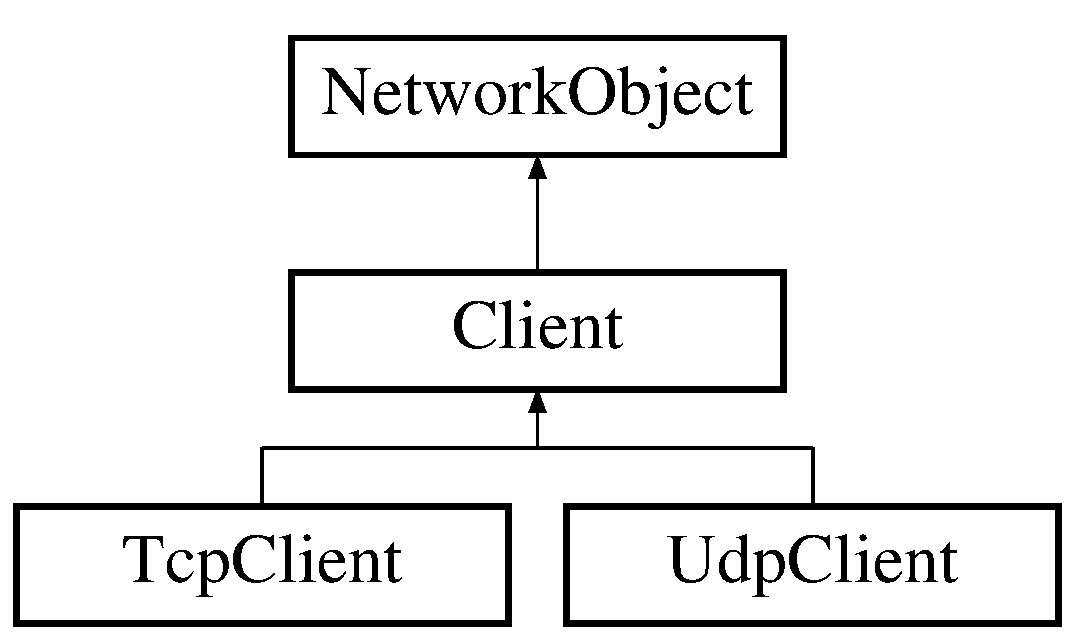
\includegraphics[height=3.000000cm]{classClient}
\end{center}
\end{figure}
\subsection*{Public Member Functions}
\begin{DoxyCompactItemize}
\item 
\hyperlink{classClient_ae51af7aa6b8f591496a8f6a4a87a14bf}{Client} ()
\item 
virtual \hyperlink{classClient_a897ff0f31827f7be3c661623341605ed}{$\sim$Client} ()
\item 
virtual void \hyperlink{classClient_ae02f1c7ffac49b7543244da28fbb58aa}{send} (const string \&data)=0
\item 
virtual void \hyperlink{classClient_a6d77759bc7022e45a3e4326757bd6b8b}{send\_\-bytes} (const vector$<$ \hyperlink{Event_8h_ae0aa21f6bcb621fe36c2c962aa0452fe}{byte} $>$ \&bytes)=0
\item 
virtual string \hyperlink{classClient_a01e5ea1bae012b2a46e8abd6b0bab704}{get\_\-host} ()=0
\item 
virtual int \hyperlink{classClient_ac9e4f13eef6b9a776b2bb6cca9d4f78b}{get\_\-port} ()=0
\item 
\hyperlink{classClient_a382edd74d967440910a27735d6d83ad9}{FB\_\-JSAPI\_\-EVENT} (resolve, 0,())
\end{DoxyCompactItemize}


\subsection{Detailed Description}
An abstract interface for a client object. This registers the generic client-\/specific events to javascript, and registers the 'send' method to the javascript API. 

Definition at line 17 of file Client.h.



\subsection{Constructor \& Destructor Documentation}
\hypertarget{classClient_ae51af7aa6b8f591496a8f6a4a87a14bf}{
\index{Client@{Client}!Client@{Client}}
\index{Client@{Client}!Client@{Client}}
\subsubsection[{Client}]{\setlength{\rightskip}{0pt plus 5cm}Client::Client (
\begin{DoxyParamCaption}
{}
\end{DoxyParamCaption}
)}}
\label{classClient_ae51af7aa6b8f591496a8f6a4a87a14bf}
Constructs a default client object by registering the 'send' method for this client to the javascript. 

Definition at line 10 of file Client.cpp.



References get\_\-host(), get\_\-port(), send(), and send\_\-bytes().


\begin{DoxyCode}
{
    registerMethod("send", make_method(this, &Client::send));
    registerMethod("sendBytes", make_method(this, &Client::send_bytes));
    registerMethod("getHost", make_method(this, &Client::get_host));
    registerMethod("getPort", make_method(this, &Client::get_port));
}
\end{DoxyCode}
\hypertarget{classClient_a897ff0f31827f7be3c661623341605ed}{
\index{Client@{Client}!$\sim$Client@{$\sim$Client}}
\index{$\sim$Client@{$\sim$Client}!Client@{Client}}
\subsubsection[{$\sim$Client}]{\setlength{\rightskip}{0pt plus 5cm}virtual Client::$\sim$Client (
\begin{DoxyParamCaption}
{}
\end{DoxyParamCaption}
)\hspace{0.3cm}{\ttfamily  \mbox{[}inline, virtual\mbox{]}}}}
\label{classClient_a897ff0f31827f7be3c661623341605ed}
Deconstructs a client object 

Definition at line 29 of file Client.h.


\begin{DoxyCode}
{}
\end{DoxyCode}


\subsection{Member Function Documentation}
\hypertarget{classClient_a382edd74d967440910a27735d6d83ad9}{
\index{Client@{Client}!FB\_\-JSAPI\_\-EVENT@{FB\_\-JSAPI\_\-EVENT}}
\index{FB\_\-JSAPI\_\-EVENT@{FB\_\-JSAPI\_\-EVENT}!Client@{Client}}
\subsubsection[{FB\_\-JSAPI\_\-EVENT}]{\setlength{\rightskip}{0pt plus 5cm}Client::FB\_\-JSAPI\_\-EVENT (
\begin{DoxyParamCaption}
\item[{resolve}]{, }
\item[{0}]{, }
\item[{()}]{}
\end{DoxyParamCaption}
)}}
\label{classClient_a382edd74d967440910a27735d6d83ad9}
A javascript event to be fired when the client has successfully resolved the remote host name and is prepared to send data to the remote host. \hypertarget{classClient_a01e5ea1bae012b2a46e8abd6b0bab704}{
\index{Client@{Client}!get\_\-host@{get\_\-host}}
\index{get\_\-host@{get\_\-host}!Client@{Client}}
\subsubsection[{get\_\-host}]{\setlength{\rightskip}{0pt plus 5cm}virtual string Client::get\_\-host (
\begin{DoxyParamCaption}
{}
\end{DoxyParamCaption}
)\hspace{0.3cm}{\ttfamily  \mbox{[}pure virtual\mbox{]}}}}
\label{classClient_a01e5ea1bae012b2a46e8abd6b0bab704}
Get host to which this client connects

\begin{DoxyReturn}{Returns}
The host to which this client connects 
\end{DoxyReturn}


Implemented in \hyperlink{classTcpClient_a4c1ecfdba951d559456c4066a73c8bf6}{TcpClient}, and \hyperlink{classUdpClient_ac18bd8d30497c82dfe1a63a464d01e00}{UdpClient}.



Referenced by Client().

\hypertarget{classClient_ac9e4f13eef6b9a776b2bb6cca9d4f78b}{
\index{Client@{Client}!get\_\-port@{get\_\-port}}
\index{get\_\-port@{get\_\-port}!Client@{Client}}
\subsubsection[{get\_\-port}]{\setlength{\rightskip}{0pt plus 5cm}virtual int Client::get\_\-port (
\begin{DoxyParamCaption}
{}
\end{DoxyParamCaption}
)\hspace{0.3cm}{\ttfamily  \mbox{[}pure virtual\mbox{]}}}}
\label{classClient_ac9e4f13eef6b9a776b2bb6cca9d4f78b}
Get the port on the remote host to this client connects

\begin{DoxyReturn}{Returns}
The port on the remote host to which this client connects 
\end{DoxyReturn}


Implemented in \hyperlink{classTcpClient_a9caf99246bc1f36dcc69773077ddece8}{TcpClient}, and \hyperlink{classUdpClient_aaa19f0f767306e0e974782dd700c5c49}{UdpClient}.



Referenced by Client().

\hypertarget{classClient_ae02f1c7ffac49b7543244da28fbb58aa}{
\index{Client@{Client}!send@{send}}
\index{send@{send}!Client@{Client}}
\subsubsection[{send}]{\setlength{\rightskip}{0pt plus 5cm}virtual void Client::send (
\begin{DoxyParamCaption}
\item[{const string \&}]{data}
\end{DoxyParamCaption}
)\hspace{0.3cm}{\ttfamily  \mbox{[}pure virtual\mbox{]}}}}
\label{classClient_ae02f1c7ffac49b7543244da28fbb58aa}
Asynchronously sends data to the remote host to which this client is connected.


\begin{DoxyParams}{Parameters}
{\em data} & The data to send across the wire \\
\hline
\end{DoxyParams}


Implemented in \hyperlink{classTcpClient_a139cffd600eaf851c3560d73a1ba3a54}{TcpClient}, and \hyperlink{classUdpClient_a86e50f32bbb7aaf657ea5cc91cbc99d2}{UdpClient}.



Referenced by Client().

\hypertarget{classClient_a6d77759bc7022e45a3e4326757bd6b8b}{
\index{Client@{Client}!send\_\-bytes@{send\_\-bytes}}
\index{send\_\-bytes@{send\_\-bytes}!Client@{Client}}
\subsubsection[{send\_\-bytes}]{\setlength{\rightskip}{0pt plus 5cm}virtual void Client::send\_\-bytes (
\begin{DoxyParamCaption}
\item[{const vector$<$ {\bf byte} $>$ \&}]{bytes}
\end{DoxyParamCaption}
)\hspace{0.3cm}{\ttfamily  \mbox{[}pure virtual\mbox{]}}}}
\label{classClient_a6d77759bc7022e45a3e4326757bd6b8b}
Asynchronously sends bytes to the remote host to which this client is connected.


\begin{DoxyParams}{Parameters}
{\em bytes} & The bytes of data to send across the wire \\
\hline
\end{DoxyParams}


Implemented in \hyperlink{classTcpClient_a1d749cbc2e255d8d3204dfd2d2c58d5f}{TcpClient}, and \hyperlink{classUdpClient_ad55f42a3c5cb3698b49975c8a065079e}{UdpClient}.



Referenced by Client().



The documentation for this class was generated from the following files:\begin{DoxyCompactItemize}
\item 
/home/jtedesco/dev/sockit/src/common/\hyperlink{Client_8h}{Client.h}\item 
/home/jtedesco/dev/sockit/src/common/\hyperlink{Client_8cpp}{Client.cpp}\end{DoxyCompactItemize}

\hypertarget{classEvent}{
\section{Event Class Reference}
\label{classEvent}\index{Event@{Event}}
}


{\ttfamily \#include $<$Event.h$>$}

Inheritance diagram for Event:\begin{figure}[H]
\begin{center}
\leavevmode
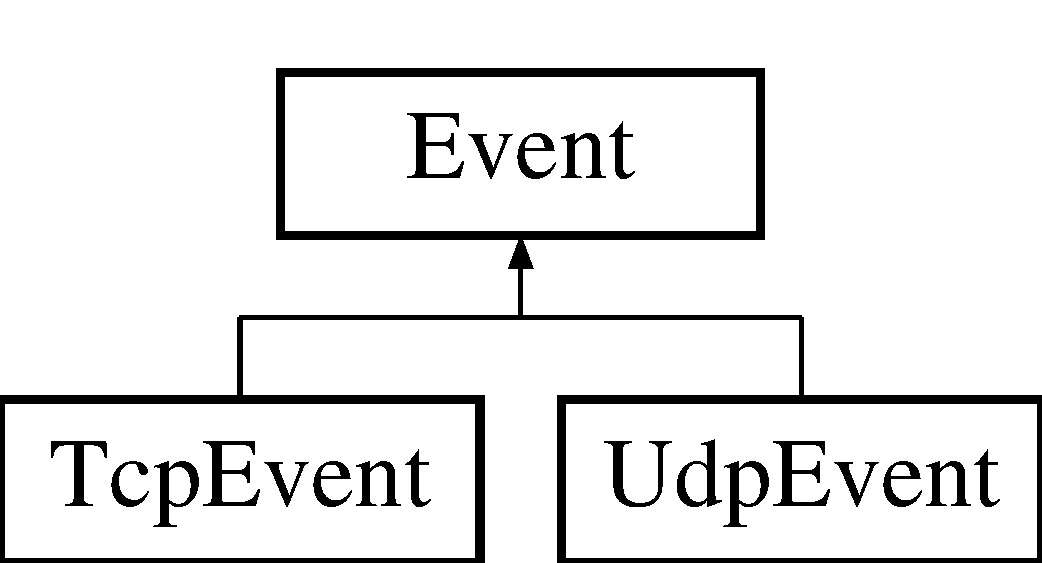
\includegraphics[height=2.000000cm]{classEvent}
\end{center}
\end{figure}
\subsection*{Public Member Functions}
\begin{DoxyCompactItemize}
\item 
\hyperlink{classEvent_a5a40dd4708297f7031e29b39e039ae10}{Event} ()
\item 
virtual \hyperlink{classEvent_a7704ec01ce91e673885792054214b3d2}{$\sim$Event} ()
\item 
virtual void \hyperlink{classEvent_ac4eac8e7d44356632b59381929c8978c}{send} (const string \&data)=0
\item 
virtual void \hyperlink{classEvent_ac2183e14a4f65b18d046a5e082f68e71}{send\_\-bytes} (const vector$<$ \hyperlink{Event_8h_ae0aa21f6bcb621fe36c2c962aa0452fe}{byte} $>$ \&bytes)=0
\item 
virtual string \hyperlink{classEvent_a9e334d69556816ca38a8f21845d2a1cb}{read} () const =0
\item 
virtual FB::VariantList \hyperlink{classEvent_a04fa24d70fb7ec47e50e1a71bcedfe75}{read\_\-bytes} () const =0
\item 
virtual string \hyperlink{classEvent_ac3fe62061cb4e4552a91be17031fcc2d}{get\_\-host} ()=0
\item 
virtual unsigned short \hyperlink{classEvent_aa23b8454f931fcbe87ed61f1ec70b8e5}{get\_\-port} ()=0
\item 
\hyperlink{classEvent_ad77fd1b739e3291db3719f15dc44afb2}{FB\_\-JSAPI\_\-EVENT} (error, 1,(const string \&))
\end{DoxyCompactItemize}


\subsection{Detailed Description}
Generic interface used to reply to data on some connection from Javascript. 

Definition at line 29 of file Event.h.



\subsection{Constructor \& Destructor Documentation}
\hypertarget{classEvent_a5a40dd4708297f7031e29b39e039ae10}{
\index{Event@{Event}!Event@{Event}}
\index{Event@{Event}!Event@{Event}}
\subsubsection[{Event}]{\setlength{\rightskip}{0pt plus 5cm}Event::Event (
\begin{DoxyParamCaption}
{}
\end{DoxyParamCaption}
)}}
\label{classEvent_a5a40dd4708297f7031e29b39e039ae10}
Constructor that register the Javascript API for event objects 

Definition at line 10 of file Event.cpp.



References get\_\-host(), get\_\-port(), read(), read\_\-bytes(), send(), and send\_\-bytes().


\begin{DoxyCode}
{
    // Expose these methods to the Javascript
    registerMethod("send", make_method(this, &Event::send));
    registerMethod("sendBytes", make_method(this, &Event::send_bytes));
    registerMethod("read", make_method(this, &Event::read));
    registerMethod("readBytes", make_method(this, &Event::read_bytes));
    registerMethod("getHost", make_method(this, &Event::get_host));
    registerMethod("getPort", make_method(this, &Event::get_port));
}
\end{DoxyCode}
\hypertarget{classEvent_a7704ec01ce91e673885792054214b3d2}{
\index{Event@{Event}!$\sim$Event@{$\sim$Event}}
\index{$\sim$Event@{$\sim$Event}!Event@{Event}}
\subsubsection[{$\sim$Event}]{\setlength{\rightskip}{0pt plus 5cm}Event::$\sim$Event (
\begin{DoxyParamCaption}
{}
\end{DoxyParamCaption}
)\hspace{0.3cm}{\ttfamily  \mbox{[}virtual\mbox{]}}}}
\label{classEvent_a7704ec01ce91e673885792054214b3d2}
Deconstructs a event object 

Definition at line 22 of file Event.cpp.


\begin{DoxyCode}
{
    // Nothing to do here
}
\end{DoxyCode}


\subsection{Member Function Documentation}
\hypertarget{classEvent_ad77fd1b739e3291db3719f15dc44afb2}{
\index{Event@{Event}!FB\_\-JSAPI\_\-EVENT@{FB\_\-JSAPI\_\-EVENT}}
\index{FB\_\-JSAPI\_\-EVENT@{FB\_\-JSAPI\_\-EVENT}!Event@{Event}}
\subsubsection[{FB\_\-JSAPI\_\-EVENT}]{\setlength{\rightskip}{0pt plus 5cm}Event::FB\_\-JSAPI\_\-EVENT (
\begin{DoxyParamCaption}
\item[{error}]{, }
\item[{1}]{, }
\item[{(const string \&)}]{}
\end{DoxyParamCaption}
)}}
\label{classEvent_ad77fd1b739e3291db3719f15dc44afb2}
The javascript event fired when an error occurs, which sends the error message when fired. \hypertarget{classEvent_ac3fe62061cb4e4552a91be17031fcc2d}{
\index{Event@{Event}!get\_\-host@{get\_\-host}}
\index{get\_\-host@{get\_\-host}!Event@{Event}}
\subsubsection[{get\_\-host}]{\setlength{\rightskip}{0pt plus 5cm}virtual string Event::get\_\-host (
\begin{DoxyParamCaption}
{}
\end{DoxyParamCaption}
)\hspace{0.3cm}{\ttfamily  \mbox{[}pure virtual\mbox{]}}}}
\label{classEvent_ac3fe62061cb4e4552a91be17031fcc2d}
Get the address, or hostname of the remote endpoint for this event. \begin{DoxyReturn}{Returns}
The hostname of the remote endpoint for this event. 
\end{DoxyReturn}


Implemented in \hyperlink{classTcpEvent_a47be6347ecf372f3fbf934ba489d90c1}{TcpEvent}, and \hyperlink{classUdpEvent_ae2484477a11197f79d46e4ef4b71b839}{UdpEvent}.



Referenced by Event().

\hypertarget{classEvent_aa23b8454f931fcbe87ed61f1ec70b8e5}{
\index{Event@{Event}!get\_\-port@{get\_\-port}}
\index{get\_\-port@{get\_\-port}!Event@{Event}}
\subsubsection[{get\_\-port}]{\setlength{\rightskip}{0pt plus 5cm}virtual unsigned short Event::get\_\-port (
\begin{DoxyParamCaption}
{}
\end{DoxyParamCaption}
)\hspace{0.3cm}{\ttfamily  \mbox{[}pure virtual\mbox{]}}}}
\label{classEvent_aa23b8454f931fcbe87ed61f1ec70b8e5}
Get the port associated with the remote endpoint of this event. \begin{DoxyReturn}{Returns}
port The port associated with the remote endpoint of this event. 
\end{DoxyReturn}


Implemented in \hyperlink{classTcpEvent_aa14fbf8c465c3487e7eae02ec8815093}{TcpEvent}, and \hyperlink{classUdpEvent_aaad6ade41ef171993364911ed57a3185}{UdpEvent}.



Referenced by Event().

\hypertarget{classEvent_a9e334d69556816ca38a8f21845d2a1cb}{
\index{Event@{Event}!read@{read}}
\index{read@{read}!Event@{Event}}
\subsubsection[{read}]{\setlength{\rightskip}{0pt plus 5cm}virtual string Event::read (
\begin{DoxyParamCaption}
{}
\end{DoxyParamCaption}
) const\hspace{0.3cm}{\ttfamily  \mbox{[}pure virtual\mbox{]}}}}
\label{classEvent_a9e334d69556816ca38a8f21845d2a1cb}
Reads the string data that belongs to this event.

\begin{DoxyReturn}{Returns}
The string data received when this event was fired 
\end{DoxyReturn}


Implemented in \hyperlink{classTcpEvent_abc8541d2f0e5b0fbf15191392fbb4a20}{TcpEvent}, and \hyperlink{classUdpEvent_a860ceb7a3a8bb6fcd7cb1342d8b7f5c7}{UdpEvent}.



Referenced by Event().

\hypertarget{classEvent_a04fa24d70fb7ec47e50e1a71bcedfe75}{
\index{Event@{Event}!read\_\-bytes@{read\_\-bytes}}
\index{read\_\-bytes@{read\_\-bytes}!Event@{Event}}
\subsubsection[{read\_\-bytes}]{\setlength{\rightskip}{0pt plus 5cm}virtual FB::VariantList Event::read\_\-bytes (
\begin{DoxyParamCaption}
{}
\end{DoxyParamCaption}
) const\hspace{0.3cm}{\ttfamily  \mbox{[}pure virtual\mbox{]}}}}
\label{classEvent_a04fa24d70fb7ec47e50e1a71bcedfe75}
Reads the byte data that belongs to this event

\begin{DoxyReturn}{Returns}
The byte data received when this event was fired 
\end{DoxyReturn}


Implemented in \hyperlink{classTcpEvent_adcbbf4231886db58d1df95357b249a26}{TcpEvent}, and \hyperlink{classUdpEvent_ad315a9d5969bc5d38f3d592119cac9ca}{UdpEvent}.



Referenced by Event().

\hypertarget{classEvent_ac4eac8e7d44356632b59381929c8978c}{
\index{Event@{Event}!send@{send}}
\index{send@{send}!Event@{Event}}
\subsubsection[{send}]{\setlength{\rightskip}{0pt plus 5cm}virtual void Event::send (
\begin{DoxyParamCaption}
\item[{const string \&}]{data}
\end{DoxyParamCaption}
)\hspace{0.3cm}{\ttfamily  \mbox{[}pure virtual\mbox{]}}}}
\label{classEvent_ac4eac8e7d44356632b59381929c8978c}
Reply on this {\ttfamily \hyperlink{classEvent}{Event}}'s connection with some data.


\begin{DoxyParams}{Parameters}
{\em data} & The data to send \\
\hline
\end{DoxyParams}


Implemented in \hyperlink{classTcpEvent_ac9e73ac6ebadc8712d3edfec5e4b1dc9}{TcpEvent}, and \hyperlink{classUdpEvent_a1f88c17a020ccf73a61a40d18b3728a0}{UdpEvent}.



Referenced by Event().

\hypertarget{classEvent_ac2183e14a4f65b18d046a5e082f68e71}{
\index{Event@{Event}!send\_\-bytes@{send\_\-bytes}}
\index{send\_\-bytes@{send\_\-bytes}!Event@{Event}}
\subsubsection[{send\_\-bytes}]{\setlength{\rightskip}{0pt plus 5cm}virtual void Event::send\_\-bytes (
\begin{DoxyParamCaption}
\item[{const vector$<$ {\bf byte} $>$ \&}]{bytes}
\end{DoxyParamCaption}
)\hspace{0.3cm}{\ttfamily  \mbox{[}pure virtual\mbox{]}}}}
\label{classEvent_ac2183e14a4f65b18d046a5e082f68e71}
Reply on this {\ttfamily \hyperlink{classEvent}{Event}}'s connection with some data, given as bytes.


\begin{DoxyParams}{Parameters}
{\em bytes} & The bytes of data with which to reply \\
\hline
\end{DoxyParams}


Implemented in \hyperlink{classTcpEvent_ab6741ad9135b421c220e7601939ea925}{TcpEvent}, and \hyperlink{classUdpEvent_ac44fcd996dd22e49d7dd7721198f7550}{UdpEvent}.



Referenced by Event().



The documentation for this class was generated from the following files:\begin{DoxyCompactItemize}
\item 
/home/jtedesco/dev/sockit/src/common/\hyperlink{Event_8h}{Event.h}\item 
/home/jtedesco/dev/sockit/src/common/\hyperlink{Event_8cpp}{Event.cpp}\end{DoxyCompactItemize}

\hypertarget{classLogger}{
\section{Logger Class Reference}
\label{classLogger}\index{Logger@{Logger}}
}


{\ttfamily \#include $<$Logger.h$>$}

\subsection*{Static Public Member Functions}
\begin{DoxyCompactItemize}
\item 
static void \hyperlink{classLogger_adb709be72ac3e448f2af97b9cafaef2f}{error} (string msg, int port=\hyperlink{classLogger_a5ec2e368c2190d33a096925d96309b32}{NO\_\-PORT}, string host=\char`\"{}local\char`\"{})
\item 
static void \hyperlink{classLogger_a8c7d9b42b9a5480dceed15a21a2d57c6}{info} (string msg, int port=\hyperlink{classLogger_a5ec2e368c2190d33a096925d96309b32}{NO\_\-PORT}, string host=\char`\"{}local\char`\"{})
\item 
static void \hyperlink{classLogger_ae0ebb73647360cb425de15cb9790563d}{warn} (string msg, int port=\hyperlink{classLogger_a5ec2e368c2190d33a096925d96309b32}{NO\_\-PORT}, string host=\char`\"{}local\char`\"{})
\item 
static const bool \hyperlink{classLogger_a29dfeca29285b06316a9644347ba480b}{is\_\-enabled} ()
\item 
static void \hyperlink{classLogger_a9dbb809282232adfbe81a780077e587a}{shutdown} ()
\end{DoxyCompactItemize}
\subsection*{Static Public Attributes}
\begin{DoxyCompactItemize}
\item 
static const int \hyperlink{classLogger_a5ec2e368c2190d33a096925d96309b32}{NO\_\-PORT} = 0
\end{DoxyCompactItemize}
\subsection*{Private Member Functions}
\begin{DoxyCompactItemize}
\item 
\hyperlink{classLogger_abc41bfb031d896170c7675fa96a6b30c}{Logger} ()
\end{DoxyCompactItemize}
\subsection*{Static Private Member Functions}
\begin{DoxyCompactItemize}
\item 
static void \hyperlink{classLogger_a28f4a9602314326324efe66cb080b9cd}{queue} (string host, int port, string msg, string cat)
\item 
static string \hyperlink{classLogger_ab029553d98fef32a959c4dd9a9d54eea}{get\_\-date} ()
\item 
static string \hyperlink{classLogger_a227293d7b2941454b62fbb5471711200}{get\_\-timestamp} ()
\item 
static string \hyperlink{classLogger_a3bbf4bde3c17ce025625efdc3651d62a}{get\_\-log\_\-base\_\-path} ()
\item 
static void \hyperlink{classLogger_ae784283f1de7827b7e7049641eaf0a53}{initialize} ()
\item 
static void \hyperlink{classLogger_af1ed54470b81ee4e42d846f0b42e8789}{log\_\-writer\_\-run} ()
\item 
static void \hyperlink{classLogger_a5860ff086efc6bf785ac9e62f4f5bcad}{handle\_\-write\_\-request} (string dir, string line)
\item 
static void \hyperlink{classLogger_a7c152c7936d69ffa5de724143ba39f58}{formatter\_\-run} ()
\item 
static void \hyperlink{classLogger_a8dda3deb5412352e1fea15c000318404}{handle\_\-format\_\-request} (string host, int port, string msg, string cat)
\end{DoxyCompactItemize}
\subsection*{Static Private Attributes}
\begin{DoxyCompactItemize}
\item 
static const int \hyperlink{classLogger_a7bd8d738b20738225377ac59e47792e5}{SLEEP\_\-TIME\_\-MS} = 50
\item 
static bool \hyperlink{classLogger_aef732b653322fdd9ba7b0a72e90814a4}{initialized} = false
\item 
static bool \hyperlink{classLogger_adaefa0ae12070af07bb69aed1a3d0b31}{enabled} = true
\item 
static boost::mutex \hyperlink{classLogger_a2c4c569c9b4e1d3161979e4d60545024}{log\_\-writer\_\-mtx}
\item 
static boost::mutex \hyperlink{classLogger_a5114b8ee8bc6f37b217aa8c36d5a342d}{formatter\_\-mtx}
\item 
static boost::mutex \hyperlink{classLogger_a3438c31e00d8260e58269d57e2526533}{shutdown\_\-mtx}
\item 
static boost::condition\_\-variable \hyperlink{classLogger_a62912b685f72e2782371d0867b2d23f7}{shutdown\_\-cvar}
\item 
static boost::condition\_\-variable \hyperlink{classLogger_a07fe7895664750eb3bf6b0cb39034182}{formatter\_\-cvar}
\item 
static boost::condition\_\-variable \hyperlink{classLogger_afbd56cc7017de01fc22be29f641be63a}{log\_\-writer\_\-cvar}
\item 
static std::queue$<$ pair$<$ pair$<$ string, int $>$, pair$<$ string, string $>$ $>$ $>$ \hyperlink{classLogger_aeef2780f8f49da507fb3c954a1cdae29}{raw\_\-requests}
\item 
static std::queue$<$ pair$<$ string, string $>$ $>$ \hyperlink{classLogger_ac6f7534f905bc9b903b35549fa526688}{write\_\-requests}
\item 
static string \hyperlink{classLogger_a0fe7f2c4dcb22ef87f07294f3db9d8cc}{pid}
\item 
static boost::thread \hyperlink{classLogger_a46e8969c902a456bee9802196044f582}{frm\_\-t}
\item 
static boost::thread \hyperlink{classLogger_a6214da297e928d0c9f960a249b6fcf8c}{lw\_\-t}
\end{DoxyCompactItemize}


\subsection{Detailed Description}
\hyperlink{Logger_8h}{Logger.h}

Do not instantiate or inherit from this class.

An asynchronous logger. Call by using {\ttfamily \hyperlink{classLogger_a8c7d9b42b9a5480dceed15a21a2d57c6}{Logger::info}(\char`\"{}msg\char`\"{});} or equivalent method. Designed to have the main thread do as little work as possible.

Internally, there are two background threads. One formats a log request into a file directory and a log entry. The other actually writes this into the log. Hopefully, one thread can be in a system call (to get the current date or time) and the other can be doing I/O.

Sadly, a bug in firebreath+boost prevents both background threads from sleeping and just periodically checking that there's work. The bug makes the sleeping thread hang indefinitely (until interrupted). Since the bug affects waiting/timed waiting on a condition variable, (which is how boost implements sleep), the main thread has to signal the formatter thread just in case the bug happened. The formatter thread then signals the log writing thread when there's work.

Logs are placed in /sockit/YYYY-\/MM-\/DD/REMOTEHOST/PROCESSID/sockit-\/traffic.log.

Note: \hyperlink{classLogger_a9dbb809282232adfbe81a780077e587a}{Logger::shutdown()} should only be called once, when the plugin is shutting down. After this is called, no more logging will take place. 

Definition at line 60 of file Logger.h.



\subsection{Constructor \& Destructor Documentation}
\hypertarget{classLogger_abc41bfb031d896170c7675fa96a6b30c}{
\index{Logger@{Logger}!Logger@{Logger}}
\index{Logger@{Logger}!Logger@{Logger}}
\subsubsection[{Logger}]{\setlength{\rightskip}{0pt plus 5cm}Logger::Logger (
\begin{DoxyParamCaption}
{}
\end{DoxyParamCaption}
)\hspace{0.3cm}{\ttfamily  \mbox{[}inline, private\mbox{]}}}}
\label{classLogger_abc41bfb031d896170c7675fa96a6b30c}


Definition at line 122 of file Logger.h.


\begin{DoxyCode}
        {
        }
\end{DoxyCode}


\subsection{Member Function Documentation}
\hypertarget{classLogger_adb709be72ac3e448f2af97b9cafaef2f}{
\index{Logger@{Logger}!error@{error}}
\index{error@{error}!Logger@{Logger}}
\subsubsection[{error}]{\setlength{\rightskip}{0pt plus 5cm}static void Logger::error (
\begin{DoxyParamCaption}
\item[{string}]{msg, }
\item[{int}]{port = {\ttfamily {\bf NO\_\-PORT}}, }
\item[{string}]{host = {\ttfamily \char`\"{}local\char`\"{}}}
\end{DoxyParamCaption}
)\hspace{0.3cm}{\ttfamily  \mbox{[}inline, static\mbox{]}}}}
\label{classLogger_adb709be72ac3e448f2af97b9cafaef2f}
Log that there is an error, along with a message.


\begin{DoxyParams}{Parameters}
{\em host} & Either a client's remote host or the localhost for servers \\
\hline
{\em port} & Either the remote host's port (for a client) or the server's local port \\
\hline
{\em msg} & The message to log \\
\hline
\end{DoxyParams}


Definition at line 71 of file Logger.h.



References is\_\-enabled(), and queue().



Referenced by TcpServer::accept\_\-handler(), TcpClient::connect\_\-handler(), TcpServer::init(), TcpClient::init(), UdpClient::init\_\-socket(), UdpServer::initialize(), Udp::receive\_\-handler(), Tcp::receive\_\-handler(), UdpClient::resolve\_\-handler(), TcpClient::resolve\_\-handler(), NetworkThread::run(), UdpEvent::send(), UdpClient::send(), TcpEvent::send(), TcpClient::send(), Udp::send\_\-handler(), Tcp::send\_\-handler(), Tcp::set\_\-tcp\_\-keepalive(), UdpServer::shutdown(), TcpServer::shutdown(), TcpClient::shutdown(), socket\_\-deallocate(), UdpServer::start\_\-listening(), TcpServer::start\_\-listening(), TcpClient::TcpClient(), TcpEvent::TcpEvent(), UdpClient::UdpClient(), and UdpEvent::UdpEvent().


\begin{DoxyCode}
        {
            if (Logger::is_enabled())
                Logger::queue(host, port, msg, "ERROR :  ");
        }
\end{DoxyCode}
\hypertarget{classLogger_a7c152c7936d69ffa5de724143ba39f58}{
\index{Logger@{Logger}!formatter\_\-run@{formatter\_\-run}}
\index{formatter\_\-run@{formatter\_\-run}!Logger@{Logger}}
\subsubsection[{formatter\_\-run}]{\setlength{\rightskip}{0pt plus 5cm}void Logger::formatter\_\-run (
\begin{DoxyParamCaption}
{}
\end{DoxyParamCaption}
)\hspace{0.3cm}{\ttfamily  \mbox{[}static, private\mbox{]}}}}
\label{classLogger_a7c152c7936d69ffa5de724143ba39f58}
Only the formatter thread should be here. Run until logging is disabled and handle formatting requests. 

Definition at line 130 of file Logger.cpp.



References enabled, formatter\_\-cvar, formatter\_\-mtx, handle\_\-format\_\-request(), raw\_\-requests, and SLEEP\_\-TIME\_\-MS.



Referenced by initialize().


\begin{DoxyCode}
{
    // needed for sleeping on a boost cvar
    boost::unique_lock<boost::mutex> fmt_lock(formatter_mtx);

    // continue as long as logging is enabled and there are still raw requests to
       process
    while(true)
    {
        while (!raw_requests.empty())
        {
            // handle one request
            pair<pair<string, int> , pair<string, string> > p = raw_requests.fron
      t();
            raw_requests.pop();
            fmt_lock.unlock();
            handle_format_request(p.first.first, p.first.second, p.second.first, 
      p.second.second);
            fmt_lock.lock();
        }
       
        if(enabled || !raw_requests.empty()) 
        {
            // Sigh. There's a bug with firebreath + boost::this_thread::sleep/bo
      ost::condition_variable.timed_wait
            // where the sleeping thread hangs forever. So this is a compromise/w
      ork around.

            // don't hold the lock across the gettime system call
            fmt_lock.unlock();
            boost::system_time sleep_time = boost::get_system_time() + boost::pos
      ix_time::milliseconds(SLEEP_TIME_MS);
            fmt_lock.lock();

            // wake up periodically to check for work.
            formatter_cvar.timed_wait(fmt_lock, sleep_time);
        }
        else
        {
            fmt_lock.unlock();
            break;
        }
    }
}
\end{DoxyCode}
\hypertarget{classLogger_ab029553d98fef32a959c4dd9a9d54eea}{
\index{Logger@{Logger}!get\_\-date@{get\_\-date}}
\index{get\_\-date@{get\_\-date}!Logger@{Logger}}
\subsubsection[{get\_\-date}]{\setlength{\rightskip}{0pt plus 5cm}string Logger::get\_\-date (
\begin{DoxyParamCaption}
{}
\end{DoxyParamCaption}
)\hspace{0.3cm}{\ttfamily  \mbox{[}static, private\mbox{]}}}}
\label{classLogger_ab029553d98fef32a959c4dd9a9d54eea}
Helper for building the directory path. Gets the current date (local time) in YYYY-\/MM-\/DD format. 

Definition at line 65 of file Logger.cpp.



Referenced by handle\_\-format\_\-request().


\begin{DoxyCode}
{
    boost::gregorian::date d(boost::gregorian::day_clock::local_day());
    return boost::gregorian::to_iso_extended_string(d);
}
\end{DoxyCode}
\hypertarget{classLogger_a3bbf4bde3c17ce025625efdc3651d62a}{
\index{Logger@{Logger}!get\_\-log\_\-base\_\-path@{get\_\-log\_\-base\_\-path}}
\index{get\_\-log\_\-base\_\-path@{get\_\-log\_\-base\_\-path}!Logger@{Logger}}
\subsubsection[{get\_\-log\_\-base\_\-path}]{\setlength{\rightskip}{0pt plus 5cm}string Logger::get\_\-log\_\-base\_\-path (
\begin{DoxyParamCaption}
{}
\end{DoxyParamCaption}
)\hspace{0.3cm}{\ttfamily  \mbox{[}static, private\mbox{]}}}}
\label{classLogger_a3bbf4bde3c17ce025625efdc3651d62a}
Helper for building the directory path. Gets the base log path. 

Definition at line 79 of file Logger.cpp.



References PROFILE\_\-BUF\_\-LEN.



Referenced by handle\_\-format\_\-request().


\begin{DoxyCode}
{
#if defined (__UNIX__) || defined (__OSX__)

    string path(getenv("HOME"));

#else

#define PROFILE_BUF_LEN 250
    char profilepath[PROFILE_BUF_LEN];
    ExpandEnvironmentStringsA("%USERPROFILE%", profilepath, PROFILE_BUF_LEN);
    string path(profilepath);

#endif
    path.append("/sockit");
    return path;
}
\end{DoxyCode}
\hypertarget{classLogger_a227293d7b2941454b62fbb5471711200}{
\index{Logger@{Logger}!get\_\-timestamp@{get\_\-timestamp}}
\index{get\_\-timestamp@{get\_\-timestamp}!Logger@{Logger}}
\subsubsection[{get\_\-timestamp}]{\setlength{\rightskip}{0pt plus 5cm}string Logger::get\_\-timestamp (
\begin{DoxyParamCaption}
{}
\end{DoxyParamCaption}
)\hspace{0.3cm}{\ttfamily  \mbox{[}static, private\mbox{]}}}}
\label{classLogger_a227293d7b2941454b62fbb5471711200}
Helper for building the directory path. Gets the current timestamp (local time) in HH:MM:SS format 

Definition at line 72 of file Logger.cpp.



Referenced by handle\_\-format\_\-request().


\begin{DoxyCode}
{
    boost::posix_time::ptime now = boost::posix_time::second_clock::local_time();
      
    return boost::posix_time::to_simple_string(now);
}
\end{DoxyCode}
\hypertarget{classLogger_a8dda3deb5412352e1fea15c000318404}{
\index{Logger@{Logger}!handle\_\-format\_\-request@{handle\_\-format\_\-request}}
\index{handle\_\-format\_\-request@{handle\_\-format\_\-request}!Logger@{Logger}}
\subsubsection[{handle\_\-format\_\-request}]{\setlength{\rightskip}{0pt plus 5cm}void Logger::handle\_\-format\_\-request (
\begin{DoxyParamCaption}
\item[{string}]{host, }
\item[{int}]{port, }
\item[{string}]{msg, }
\item[{string}]{cat}
\end{DoxyParamCaption}
)\hspace{0.3cm}{\ttfamily  \mbox{[}static, private\mbox{]}}}}
\label{classLogger_a8dda3deb5412352e1fea15c000318404}
Only the formatter thread should be here. Handles a format request. 

Definition at line 170 of file Logger.cpp.



References get\_\-date(), get\_\-log\_\-base\_\-path(), get\_\-timestamp(), log\_\-writer\_\-cvar, log\_\-writer\_\-mtx, NO\_\-PORT, pid, and write\_\-requests.



Referenced by formatter\_\-run().


\begin{DoxyCode}
{
    // used to build the log path
    string host_str = (host == "local" ? "localhost" : host);
    string port_str = (port == NO_PORT ? "" : boost::lexical_cast<string>(port));
      

    string day = get_date();
    string time = get_timestamp();

    // figure out the path for this message
    string log_path(get_log_base_path() + "/" + day + "/" + host_str + "/" + pid)
      ;
    string entry(cat + "[" + time + "] " + "[" + host_str + (port == NO_PORT ? "]
       " : "] [" + port_str + "] ") + msg);

    // log request item
    pair<string, string> item(log_path, entry);

    // add item to log write queue
    log_writer_mtx.lock();
    write_requests.push(item);

    // awaken log writing thread - it has work
    log_writer_mtx.unlock();
    log_writer_cvar.notify_one();
}
\end{DoxyCode}
\hypertarget{classLogger_a5860ff086efc6bf785ac9e62f4f5bcad}{
\index{Logger@{Logger}!handle\_\-write\_\-request@{handle\_\-write\_\-request}}
\index{handle\_\-write\_\-request@{handle\_\-write\_\-request}!Logger@{Logger}}
\subsubsection[{handle\_\-write\_\-request}]{\setlength{\rightskip}{0pt plus 5cm}void Logger::handle\_\-write\_\-request (
\begin{DoxyParamCaption}
\item[{string}]{dir, }
\item[{string}]{line}
\end{DoxyParamCaption}
)\hspace{0.3cm}{\ttfamily  \mbox{[}static, private\mbox{]}}}}
\label{classLogger_a5860ff086efc6bf785ac9e62f4f5bcad}
Only the log writing thread should be in this function. Handles a log write request. 

Definition at line 238 of file Logger.cpp.



Referenced by log\_\-writer\_\-run().


\begin{DoxyCode}
{
    namespace fs = boost::filesystem;

    if (!fs::exists(dir))
    {
        try
        {
            fs::create_directories(dir);
        } catch (fs::filesystem_error &err)
        {
            // hope someone is listening..
            std::cout << "Error: could not create directory " << dir << std::endl
      ;
            return;
        }
    }

    string fileName(dir + "/sockit-traffic.log");
    line.append("\n");

    FILE *fp = fopen(fileName.c_str(), "a");

    if(fp)
    {
        fwrite(line.c_str(), line.size(), 1,  fp);
        fclose(fp);
    }
    else
    {
        std::cout << "Error: could not open file " << fileName << std::endl;
    }
}
\end{DoxyCode}
\hypertarget{classLogger_a8c7d9b42b9a5480dceed15a21a2d57c6}{
\index{Logger@{Logger}!info@{info}}
\index{info@{info}!Logger@{Logger}}
\subsubsection[{info}]{\setlength{\rightskip}{0pt plus 5cm}static void Logger::info (
\begin{DoxyParamCaption}
\item[{string}]{msg, }
\item[{int}]{port = {\ttfamily {\bf NO\_\-PORT}}, }
\item[{string}]{host = {\ttfamily \char`\"{}local\char`\"{}}}
\end{DoxyParamCaption}
)\hspace{0.3cm}{\ttfamily  \mbox{[}inline, static\mbox{]}}}}
\label{classLogger_a8c7d9b42b9a5480dceed15a21a2d57c6}
Write low-\/priority information to the log.


\begin{DoxyParams}{Parameters}
{\em host} & Either a client's remote host or the localhost for servers \\
\hline
{\em port} & Either the remote host's port (for a client) or the server's local port \\
\hline
{\em msg} & The message to log \\
\hline
\end{DoxyParams}


Definition at line 84 of file Logger.h.



References is\_\-enabled(), and queue().



Referenced by TcpServer::accept\_\-handler(), TcpClient::connect\_\-handler(), NetworkThread::create\_\-tcp\_\-client(), NetworkThread::create\_\-tcp\_\-server(), NetworkThread::create\_\-udp\_\-client(), NetworkThread::create\_\-udp\_\-server(), TcpClient::init(), UdpClient::init\_\-socket(), UdpServer::listen(), Udp::log\_\-options(), Tcp::log\_\-options(), NetworkThread::NetworkThread(), Udp::receive\_\-handler(), Tcp::receive\_\-handler(), UdpClient::resolve\_\-handler(), TcpClient::resolve\_\-handler(), UdpClient::send(), Udp::send\_\-handler(), Tcp::send\_\-handler(), UdpServer::start\_\-listening(), and TcpServer::start\_\-listening().


\begin{DoxyCode}
        {
            if (Logger::is_enabled())
                Logger::queue(host, port, msg, "INFO  :  ");
        }
\end{DoxyCode}
\hypertarget{classLogger_ae784283f1de7827b7e7049641eaf0a53}{
\index{Logger@{Logger}!initialize@{initialize}}
\index{initialize@{initialize}!Logger@{Logger}}
\subsubsection[{initialize}]{\setlength{\rightskip}{0pt plus 5cm}void Logger::initialize (
\begin{DoxyParamCaption}
{}
\end{DoxyParamCaption}
)\hspace{0.3cm}{\ttfamily  \mbox{[}static, private\mbox{]}}}}
\label{classLogger_ae784283f1de7827b7e7049641eaf0a53}
Initialize the background logging thread. Should only be called once. 

Definition at line 56 of file Logger.cpp.



References formatter\_\-run(), frm\_\-t, initialized, log\_\-writer\_\-run(), and lw\_\-t.



Referenced by queue().


\begin{DoxyCode}
{
    initialized = true;

    frm_t = boost::thread(&Logger::formatter_run);
    lw_t = boost::thread(&Logger::log_writer_run);
}
\end{DoxyCode}
\hypertarget{classLogger_a29dfeca29285b06316a9644347ba480b}{
\index{Logger@{Logger}!is\_\-enabled@{is\_\-enabled}}
\index{is\_\-enabled@{is\_\-enabled}!Logger@{Logger}}
\subsubsection[{is\_\-enabled}]{\setlength{\rightskip}{0pt plus 5cm}static const bool Logger::is\_\-enabled (
\begin{DoxyParamCaption}
{}
\end{DoxyParamCaption}
)\hspace{0.3cm}{\ttfamily  \mbox{[}inline, static\mbox{]}}}}
\label{classLogger_a29dfeca29285b06316a9644347ba480b}
Returns true if logging is enabled (default). Returns false if the shutdown method has been called (and logging has been disabled). 

Definition at line 107 of file Logger.h.



References enabled.



Referenced by error(), info(), and warn().


\begin{DoxyCode}
        {
            return Logger::enabled;
        }
\end{DoxyCode}
\hypertarget{classLogger_af1ed54470b81ee4e42d846f0b42e8789}{
\index{Logger@{Logger}!log\_\-writer\_\-run@{log\_\-writer\_\-run}}
\index{log\_\-writer\_\-run@{log\_\-writer\_\-run}!Logger@{Logger}}
\subsubsection[{log\_\-writer\_\-run}]{\setlength{\rightskip}{0pt plus 5cm}void Logger::log\_\-writer\_\-run (
\begin{DoxyParamCaption}
{}
\end{DoxyParamCaption}
)\hspace{0.3cm}{\ttfamily  \mbox{[}static, private\mbox{]}}}}
\label{classLogger_af1ed54470b81ee4e42d846f0b42e8789}
Only the log writing thread should be in this function. Run until logging is disabled and handle log writing requests. 

Definition at line 197 of file Logger.cpp.



References enabled, handle\_\-write\_\-request(), log\_\-writer\_\-cvar, log\_\-writer\_\-mtx, raw\_\-requests, shutdown\_\-cvar, SLEEP\_\-TIME\_\-MS, and write\_\-requests.



Referenced by initialize().


\begin{DoxyCode}
{
    // Needed to sleep on a boost cvar
    boost::unique_lock<boost::mutex> lw_lock(log_writer_mtx);

    // continue as long as logging is enabled and there are either
    // raw requests to process or log writing requests to process
    while(true)
    {
        while (!write_requests.empty())
        {
            // handle one request
            pair<string, string> p = write_requests.front();
            write_requests.pop();
            log_writer_mtx.unlock();
            handle_write_request(p.first, p.second);
            log_writer_mtx.lock();
        }

        if(enabled || !raw_requests.empty() || !write_requests.empty())
        {
            // don't hold the lock across a system call
            lw_lock.unlock();
            boost::system_time sleep_time = boost::get_system_time() + boost::pos
      ix_time::milliseconds(SLEEP_TIME_MS);
            lw_lock.lock();

            // wait until there's work
            log_writer_cvar.timed_wait(lw_lock, sleep_time);
        }
        else
        {
            lw_lock.unlock();
            break;
        }
    }

    // notify the main thread to wake up
    shutdown_cvar.notify_all();
}
\end{DoxyCode}
\hypertarget{classLogger_a28f4a9602314326324efe66cb080b9cd}{
\index{Logger@{Logger}!queue@{queue}}
\index{queue@{queue}!Logger@{Logger}}
\subsubsection[{queue}]{\setlength{\rightskip}{0pt plus 5cm}void Logger::queue (
\begin{DoxyParamCaption}
\item[{string}]{host, }
\item[{int}]{port, }
\item[{string}]{msg, }
\item[{string}]{cat}
\end{DoxyParamCaption}
)\hspace{0.3cm}{\ttfamily  \mbox{[}static, private\mbox{]}}}}
\label{classLogger_a28f4a9602314326324efe66cb080b9cd}


Definition at line 112 of file Logger.cpp.



References formatter\_\-cvar, formatter\_\-mtx, initialize(), initialized, and raw\_\-requests.



Referenced by error(), info(), and warn().


\begin{DoxyCode}
{
    pair<string, int> item1(host, port);
    pair<string, string> item2(msg, cat);
    pair<pair<string, int> , pair<string, string> > item(item1, item2);

    formatter_mtx.lock();

    if (!Logger::initialized)
        Logger::initialize();

    raw_requests.push(item);
    formatter_cvar.notify_one();

    formatter_mtx.unlock();
}
\end{DoxyCode}
\hypertarget{classLogger_a9dbb809282232adfbe81a780077e587a}{
\index{Logger@{Logger}!shutdown@{shutdown}}
\index{shutdown@{shutdown}!Logger@{Logger}}
\subsubsection[{shutdown}]{\setlength{\rightskip}{0pt plus 5cm}void Logger::shutdown (
\begin{DoxyParamCaption}
{}
\end{DoxyParamCaption}
)\hspace{0.3cm}{\ttfamily  \mbox{[}static\mbox{]}}}}
\label{classLogger_a9dbb809282232adfbe81a780077e587a}
Dangerous. Disables logging and forces the remaining logging requests to finish. Should only be called when the plugin is shutting down. 

Definition at line 98 of file Logger.cpp.



References enabled, initialized, shutdown\_\-cvar, and shutdown\_\-mtx.


\begin{DoxyCode}
{
    // disable any more log requests and disable the background threads from slee
      ping
    enabled = false;

    if(initialized)
    {
        // wait until the log writing queue is done
        boost::unique_lock<boost::mutex> lock(shutdown_mtx);
        shutdown_cvar.wait(lock);
    }
}
\end{DoxyCode}
\hypertarget{classLogger_ae0ebb73647360cb425de15cb9790563d}{
\index{Logger@{Logger}!warn@{warn}}
\index{warn@{warn}!Logger@{Logger}}
\subsubsection[{warn}]{\setlength{\rightskip}{0pt plus 5cm}static void Logger::warn (
\begin{DoxyParamCaption}
\item[{string}]{msg, }
\item[{int}]{port = {\ttfamily {\bf NO\_\-PORT}}, }
\item[{string}]{host = {\ttfamily \char`\"{}local\char`\"{}}}
\end{DoxyParamCaption}
)\hspace{0.3cm}{\ttfamily  \mbox{[}inline, static\mbox{]}}}}
\label{classLogger_ae0ebb73647360cb425de15cb9790563d}
Log that there is an warning, along with a message.


\begin{DoxyParams}{Parameters}
{\em host} & Either a client's remote host or the localhost for servers \\
\hline
{\em port} & Either the remote host's port (for a client) or the server's local port \\
\hline
{\em msg} & The message to log \\
\hline
\end{DoxyParams}


Definition at line 97 of file Logger.h.



References is\_\-enabled(), and queue().



Referenced by TcpServer::accept\_\-handler(), TcpServer::close(), TcpClient::close(), TcpClient::connect\_\-handler(), UdpServer::listen(), UdpClient::listen(), Tcp::receive\_\-handler(), TcpClient::resolve\_\-handler(), Tcp::send\_\-handler(), and NetworkThread::$\sim$NetworkThread().


\begin{DoxyCode}
        {
            if (Logger::is_enabled())
                Logger::queue(host, port, msg, "WARN  :  ");
        }
\end{DoxyCode}


\subsection{Member Data Documentation}
\hypertarget{classLogger_adaefa0ae12070af07bb69aed1a3d0b31}{
\index{Logger@{Logger}!enabled@{enabled}}
\index{enabled@{enabled}!Logger@{Logger}}
\subsubsection[{enabled}]{\setlength{\rightskip}{0pt plus 5cm}bool {\bf Logger::enabled} = true\hspace{0.3cm}{\ttfamily  \mbox{[}static, private\mbox{]}}}}
\label{classLogger_adaefa0ae12070af07bb69aed1a3d0b31}
Enabled? 

Definition at line 160 of file Logger.h.



Referenced by formatter\_\-run(), is\_\-enabled(), log\_\-writer\_\-run(), and shutdown().

\hypertarget{classLogger_a07fe7895664750eb3bf6b0cb39034182}{
\index{Logger@{Logger}!formatter\_\-cvar@{formatter\_\-cvar}}
\index{formatter\_\-cvar@{formatter\_\-cvar}!Logger@{Logger}}
\subsubsection[{formatter\_\-cvar}]{\setlength{\rightskip}{0pt plus 5cm}boost::condition\_\-variable {\bf Logger::formatter\_\-cvar}\hspace{0.3cm}{\ttfamily  \mbox{[}static, private\mbox{]}}}}
\label{classLogger_a07fe7895664750eb3bf6b0cb39034182}
The formatter thread sleeps on this. 

Definition at line 175 of file Logger.h.



Referenced by formatter\_\-run(), and queue().

\hypertarget{classLogger_a5114b8ee8bc6f37b217aa8c36d5a342d}{
\index{Logger@{Logger}!formatter\_\-mtx@{formatter\_\-mtx}}
\index{formatter\_\-mtx@{formatter\_\-mtx}!Logger@{Logger}}
\subsubsection[{formatter\_\-mtx}]{\setlength{\rightskip}{0pt plus 5cm}boost::mutex {\bf Logger::formatter\_\-mtx}\hspace{0.3cm}{\ttfamily  \mbox{[}static, private\mbox{]}}}}
\label{classLogger_a5114b8ee8bc6f37b217aa8c36d5a342d}
Mutex for the formatter queue 

Definition at line 166 of file Logger.h.



Referenced by formatter\_\-run(), and queue().

\hypertarget{classLogger_a46e8969c902a456bee9802196044f582}{
\index{Logger@{Logger}!frm\_\-t@{frm\_\-t}}
\index{frm\_\-t@{frm\_\-t}!Logger@{Logger}}
\subsubsection[{frm\_\-t}]{\setlength{\rightskip}{0pt plus 5cm}boost::thread {\bf Logger::frm\_\-t}\hspace{0.3cm}{\ttfamily  \mbox{[}static, private\mbox{]}}}}
\label{classLogger_a46e8969c902a456bee9802196044f582}
The formatter thread 

Definition at line 190 of file Logger.h.



Referenced by initialize().

\hypertarget{classLogger_aef732b653322fdd9ba7b0a72e90814a4}{
\index{Logger@{Logger}!initialized@{initialized}}
\index{initialized@{initialized}!Logger@{Logger}}
\subsubsection[{initialized}]{\setlength{\rightskip}{0pt plus 5cm}bool {\bf Logger::initialized} = false\hspace{0.3cm}{\ttfamily  \mbox{[}static, private\mbox{]}}}}
\label{classLogger_aef732b653322fdd9ba7b0a72e90814a4}
Initialized? 

Definition at line 157 of file Logger.h.



Referenced by initialize(), queue(), and shutdown().

\hypertarget{classLogger_afbd56cc7017de01fc22be29f641be63a}{
\index{Logger@{Logger}!log\_\-writer\_\-cvar@{log\_\-writer\_\-cvar}}
\index{log\_\-writer\_\-cvar@{log\_\-writer\_\-cvar}!Logger@{Logger}}
\subsubsection[{log\_\-writer\_\-cvar}]{\setlength{\rightskip}{0pt plus 5cm}boost::condition\_\-variable {\bf Logger::log\_\-writer\_\-cvar}\hspace{0.3cm}{\ttfamily  \mbox{[}static, private\mbox{]}}}}
\label{classLogger_afbd56cc7017de01fc22be29f641be63a}
The log writer thread sleeps on this. 

Definition at line 178 of file Logger.h.



Referenced by handle\_\-format\_\-request(), and log\_\-writer\_\-run().

\hypertarget{classLogger_a2c4c569c9b4e1d3161979e4d60545024}{
\index{Logger@{Logger}!log\_\-writer\_\-mtx@{log\_\-writer\_\-mtx}}
\index{log\_\-writer\_\-mtx@{log\_\-writer\_\-mtx}!Logger@{Logger}}
\subsubsection[{log\_\-writer\_\-mtx}]{\setlength{\rightskip}{0pt plus 5cm}boost::mutex {\bf Logger::log\_\-writer\_\-mtx}\hspace{0.3cm}{\ttfamily  \mbox{[}static, private\mbox{]}}}}
\label{classLogger_a2c4c569c9b4e1d3161979e4d60545024}
Mutex for the log writer queue 

Definition at line 163 of file Logger.h.



Referenced by handle\_\-format\_\-request(), and log\_\-writer\_\-run().

\hypertarget{classLogger_a6214da297e928d0c9f960a249b6fcf8c}{
\index{Logger@{Logger}!lw\_\-t@{lw\_\-t}}
\index{lw\_\-t@{lw\_\-t}!Logger@{Logger}}
\subsubsection[{lw\_\-t}]{\setlength{\rightskip}{0pt plus 5cm}boost::thread {\bf Logger::lw\_\-t}\hspace{0.3cm}{\ttfamily  \mbox{[}static, private\mbox{]}}}}
\label{classLogger_a6214da297e928d0c9f960a249b6fcf8c}
The log-\/writer thread 

Definition at line 193 of file Logger.h.



Referenced by initialize().

\hypertarget{classLogger_a5ec2e368c2190d33a096925d96309b32}{
\index{Logger@{Logger}!NO\_\-PORT@{NO\_\-PORT}}
\index{NO\_\-PORT@{NO\_\-PORT}!Logger@{Logger}}
\subsubsection[{NO\_\-PORT}]{\setlength{\rightskip}{0pt plus 5cm}const int {\bf Logger::NO\_\-PORT} = 0\hspace{0.3cm}{\ttfamily  \mbox{[}static\mbox{]}}}}
\label{classLogger_a5ec2e368c2190d33a096925d96309b32}
no port is given 

Definition at line 117 of file Logger.h.



Referenced by NetworkThread::create\_\-tcp\_\-client(), NetworkThread::create\_\-tcp\_\-server(), NetworkThread::create\_\-udp\_\-client(), NetworkThread::create\_\-udp\_\-server(), handle\_\-format\_\-request(), NetworkThread::NetworkThread(), NetworkThread::run(), and NetworkThread::$\sim$NetworkThread().

\hypertarget{classLogger_a0fe7f2c4dcb22ef87f07294f3db9d8cc}{
\index{Logger@{Logger}!pid@{pid}}
\index{pid@{pid}!Logger@{Logger}}
\subsubsection[{pid}]{\setlength{\rightskip}{0pt plus 5cm}string {\bf Logger::pid}\hspace{0.3cm}{\ttfamily  \mbox{[}static, private\mbox{]}}}}
\label{classLogger_a0fe7f2c4dcb22ef87f07294f3db9d8cc}
The logger's pid 

Definition at line 187 of file Logger.h.



Referenced by handle\_\-format\_\-request().

\hypertarget{classLogger_aeef2780f8f49da507fb3c954a1cdae29}{
\index{Logger@{Logger}!raw\_\-requests@{raw\_\-requests}}
\index{raw\_\-requests@{raw\_\-requests}!Logger@{Logger}}
\subsubsection[{raw\_\-requests}]{\setlength{\rightskip}{0pt plus 5cm}std::queue$<$ pair$<$ pair$<$ string, int $>$, pair$<$ string, string $>$ $>$ $>$ {\bf Logger::raw\_\-requests}\hspace{0.3cm}{\ttfamily  \mbox{[}static, private\mbox{]}}}}
\label{classLogger_aeef2780f8f49da507fb3c954a1cdae29}
Queue for the raw requests 

Definition at line 181 of file Logger.h.



Referenced by formatter\_\-run(), log\_\-writer\_\-run(), and queue().

\hypertarget{classLogger_a62912b685f72e2782371d0867b2d23f7}{
\index{Logger@{Logger}!shutdown\_\-cvar@{shutdown\_\-cvar}}
\index{shutdown\_\-cvar@{shutdown\_\-cvar}!Logger@{Logger}}
\subsubsection[{shutdown\_\-cvar}]{\setlength{\rightskip}{0pt plus 5cm}boost::condition\_\-variable {\bf Logger::shutdown\_\-cvar}\hspace{0.3cm}{\ttfamily  \mbox{[}static, private\mbox{]}}}}
\label{classLogger_a62912b685f72e2782371d0867b2d23f7}
Cvar for shutting down (main thread uses this) 

Definition at line 172 of file Logger.h.



Referenced by log\_\-writer\_\-run(), and shutdown().

\hypertarget{classLogger_a3438c31e00d8260e58269d57e2526533}{
\index{Logger@{Logger}!shutdown\_\-mtx@{shutdown\_\-mtx}}
\index{shutdown\_\-mtx@{shutdown\_\-mtx}!Logger@{Logger}}
\subsubsection[{shutdown\_\-mtx}]{\setlength{\rightskip}{0pt plus 5cm}boost::mutex {\bf Logger::shutdown\_\-mtx}\hspace{0.3cm}{\ttfamily  \mbox{[}static, private\mbox{]}}}}
\label{classLogger_a3438c31e00d8260e58269d57e2526533}
Mutex for the shutdown cvar 

Definition at line 169 of file Logger.h.



Referenced by shutdown().

\hypertarget{classLogger_a7bd8d738b20738225377ac59e47792e5}{
\index{Logger@{Logger}!SLEEP\_\-TIME\_\-MS@{SLEEP\_\-TIME\_\-MS}}
\index{SLEEP\_\-TIME\_\-MS@{SLEEP\_\-TIME\_\-MS}!Logger@{Logger}}
\subsubsection[{SLEEP\_\-TIME\_\-MS}]{\setlength{\rightskip}{0pt plus 5cm}const int {\bf Logger::SLEEP\_\-TIME\_\-MS} = 50\hspace{0.3cm}{\ttfamily  \mbox{[}static, private\mbox{]}}}}
\label{classLogger_a7bd8d738b20738225377ac59e47792e5}
The formatter thread polls for work; this sets its sleep time. 

Definition at line 127 of file Logger.h.



Referenced by formatter\_\-run(), and log\_\-writer\_\-run().

\hypertarget{classLogger_ac6f7534f905bc9b903b35549fa526688}{
\index{Logger@{Logger}!write\_\-requests@{write\_\-requests}}
\index{write\_\-requests@{write\_\-requests}!Logger@{Logger}}
\subsubsection[{write\_\-requests}]{\setlength{\rightskip}{0pt plus 5cm}std::queue$<$ pair$<$ string, string $>$ $>$ {\bf Logger::write\_\-requests}\hspace{0.3cm}{\ttfamily  \mbox{[}static, private\mbox{]}}}}
\label{classLogger_ac6f7534f905bc9b903b35549fa526688}
Queue for the write requests 

Definition at line 184 of file Logger.h.



Referenced by handle\_\-format\_\-request(), and log\_\-writer\_\-run().



The documentation for this class was generated from the following files:\begin{DoxyCompactItemize}
\item 
/home/jtedesco/dev/sockit/src/logger/\hyperlink{Logger_8h}{Logger.h}\item 
/home/jtedesco/dev/sockit/src/logger/\hyperlink{Logger_8cpp}{Logger.cpp}\end{DoxyCompactItemize}

\hypertarget{classNetworkObject}{
\section{NetworkObject Class Reference}
\label{classNetworkObject}\index{NetworkObject@{NetworkObject}}
}


{\ttfamily \#include $<$NetworkObject.h$>$}

Inheritance diagram for NetworkObject:\begin{figure}[H]
\begin{center}
\leavevmode
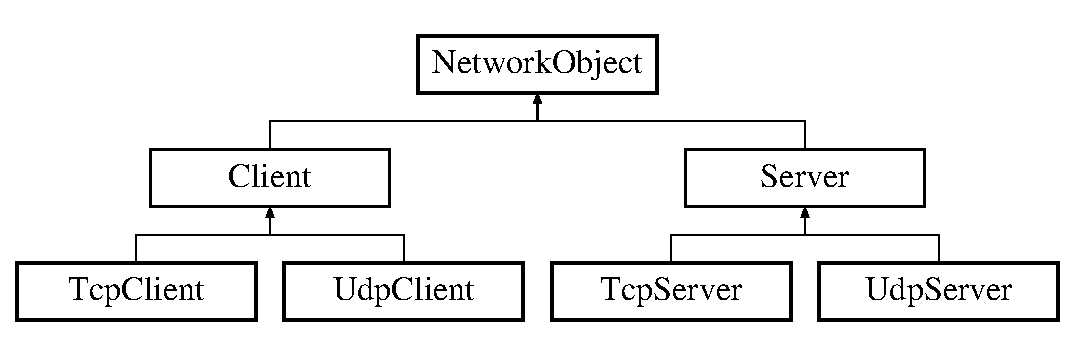
\includegraphics[height=3.000000cm]{classNetworkObject}
\end{center}
\end{figure}
\subsection*{Public Member Functions}
\begin{DoxyCompactItemize}
\item 
\hyperlink{classNetworkObject_aa317b2da072668c54e78d10b56162a6c}{NetworkObject} ()
\item 
virtual \hyperlink{classNetworkObject_aa8656ffcd38e0df2727945ac3122b4f3}{$\sim$NetworkObject} ()
\item 
virtual void \hyperlink{classNetworkObject_a2f519457fd87c8a92cf265a2b2883e96}{shutdown} ()=0
\item 
\hyperlink{classNetworkObject_a245ddfb27a8e31b8331c125a86b95d8b}{FB\_\-JSAPI\_\-EVENT} (error, 1,(const string \&))
\item 
\hyperlink{classNetworkObject_a7b5367270bfc3158309e3a3d0c353769}{FB\_\-JSAPI\_\-EVENT} (close, 0,())
\item 
\hyperlink{classNetworkObject_a6d44b6b5f6cf496af5519ddceaf93c13}{FB\_\-JSAPI\_\-EVENT} (data, 1,(FB::JSAPIPtr))
\end{DoxyCompactItemize}


\subsection{Detailed Description}


Definition at line 53 of file NetworkObject.h.



\subsection{Constructor \& Destructor Documentation}
\hypertarget{classNetworkObject_aa317b2da072668c54e78d10b56162a6c}{
\index{NetworkObject@{NetworkObject}!NetworkObject@{NetworkObject}}
\index{NetworkObject@{NetworkObject}!NetworkObject@{NetworkObject}}
\subsubsection[{NetworkObject}]{\setlength{\rightskip}{0pt plus 5cm}NetworkObject::NetworkObject (
\begin{DoxyParamCaption}
{}
\end{DoxyParamCaption}
)}}
\label{classNetworkObject_aa317b2da072668c54e78d10b56162a6c}
Constructs a generic network object by registering common events and API functions to javascript. 

Definition at line 10 of file NetworkObject.cpp.



References shutdown().


\begin{DoxyCode}
{
    registerMethod("close", make_method(this, &NetworkObject::shutdown));
}
\end{DoxyCode}
\hypertarget{classNetworkObject_aa8656ffcd38e0df2727945ac3122b4f3}{
\index{NetworkObject@{NetworkObject}!$\sim$NetworkObject@{$\sim$NetworkObject}}
\index{$\sim$NetworkObject@{$\sim$NetworkObject}!NetworkObject@{NetworkObject}}
\subsubsection[{$\sim$NetworkObject}]{\setlength{\rightskip}{0pt plus 5cm}virtual NetworkObject::$\sim$NetworkObject (
\begin{DoxyParamCaption}
{}
\end{DoxyParamCaption}
)\hspace{0.3cm}{\ttfamily  \mbox{[}inline, virtual\mbox{]}}}}
\label{classNetworkObject_aa8656ffcd38e0df2727945ac3122b4f3}
Deconstructs this network object 

Definition at line 65 of file NetworkObject.h.


\begin{DoxyCode}
{}
\end{DoxyCode}


\subsection{Member Function Documentation}
\hypertarget{classNetworkObject_a245ddfb27a8e31b8331c125a86b95d8b}{
\index{NetworkObject@{NetworkObject}!FB\_\-JSAPI\_\-EVENT@{FB\_\-JSAPI\_\-EVENT}}
\index{FB\_\-JSAPI\_\-EVENT@{FB\_\-JSAPI\_\-EVENT}!NetworkObject@{NetworkObject}}
\subsubsection[{FB\_\-JSAPI\_\-EVENT}]{\setlength{\rightskip}{0pt plus 5cm}NetworkObject::FB\_\-JSAPI\_\-EVENT (
\begin{DoxyParamCaption}
\item[{error}]{, }
\item[{1}]{, }
\item[{(const string \&)}]{}
\end{DoxyParamCaption}
)}}
\label{classNetworkObject_a245ddfb27a8e31b8331c125a86b95d8b}
The javascript event fired when an error occurs, which sends the error message when fired. \hypertarget{classNetworkObject_a6d44b6b5f6cf496af5519ddceaf93c13}{
\index{NetworkObject@{NetworkObject}!FB\_\-JSAPI\_\-EVENT@{FB\_\-JSAPI\_\-EVENT}}
\index{FB\_\-JSAPI\_\-EVENT@{FB\_\-JSAPI\_\-EVENT}!NetworkObject@{NetworkObject}}
\subsubsection[{FB\_\-JSAPI\_\-EVENT}]{\setlength{\rightskip}{0pt plus 5cm}NetworkObject::FB\_\-JSAPI\_\-EVENT (
\begin{DoxyParamCaption}
\item[{data}]{, }
\item[{1}]{, }
\item[{(FB::JSAPIPtr)}]{}
\end{DoxyParamCaption}
)}}
\label{classNetworkObject_a6d44b6b5f6cf496af5519ddceaf93c13}
The javascript event fired when the client data. This event sends with it the data received, and an object, a {\ttfamily \hyperlink{classEvent}{Event}} on which to reply to the message.

\begin{DoxySeeAlso}{See also}
\hyperlink{classEvent}{Event} 
\end{DoxySeeAlso}
\hypertarget{classNetworkObject_a7b5367270bfc3158309e3a3d0c353769}{
\index{NetworkObject@{NetworkObject}!FB\_\-JSAPI\_\-EVENT@{FB\_\-JSAPI\_\-EVENT}}
\index{FB\_\-JSAPI\_\-EVENT@{FB\_\-JSAPI\_\-EVENT}!NetworkObject@{NetworkObject}}
\subsubsection[{FB\_\-JSAPI\_\-EVENT}]{\setlength{\rightskip}{0pt plus 5cm}NetworkObject::FB\_\-JSAPI\_\-EVENT (
\begin{DoxyParamCaption}
\item[{close}]{, }
\item[{0}]{, }
\item[{()}]{}
\end{DoxyParamCaption}
)}}
\label{classNetworkObject_a7b5367270bfc3158309e3a3d0c353769}
The javascript event fired when this object shuts down. \hypertarget{classNetworkObject_a2f519457fd87c8a92cf265a2b2883e96}{
\index{NetworkObject@{NetworkObject}!shutdown@{shutdown}}
\index{shutdown@{shutdown}!NetworkObject@{NetworkObject}}
\subsubsection[{shutdown}]{\setlength{\rightskip}{0pt plus 5cm}virtual void NetworkObject::shutdown (
\begin{DoxyParamCaption}
{}
\end{DoxyParamCaption}
)\hspace{0.3cm}{\ttfamily  \mbox{[}pure virtual\mbox{]}}}}
\label{classNetworkObject_a2f519457fd87c8a92cf265a2b2883e96}
Gracefully shutdown this server object, waiting until all sends have completed before freeing all resources for this server object and shutting down any open conections. This function is exposed the javascript API. 

Implemented in \hyperlink{classTcpClient_a1f0ae8f7c7c12530bc481b77ed984790}{TcpClient}, \hyperlink{classTcpServer_a918898ee7b13d776a2f7ea8968168669}{TcpServer}, \hyperlink{classUdpClient_a64b6b51f6a2316f7235381409f9cc327}{UdpClient}, and \hyperlink{classUdpServer_ac5623ca24bc56b21d608426f5bc8ad91}{UdpServer}.



Referenced by NetworkObject().



The documentation for this class was generated from the following files:\begin{DoxyCompactItemize}
\item 
/home/jtedesco/dev/sockit/src/common/\hyperlink{NetworkObject_8h}{NetworkObject.h}\item 
/home/jtedesco/dev/sockit/src/common/\hyperlink{NetworkObject_8cpp}{NetworkObject.cpp}\end{DoxyCompactItemize}

\hypertarget{classNetworkThread}{
\section{NetworkThread Class Reference}
\label{classNetworkThread}\index{NetworkThread@{NetworkThread}}
}


{\ttfamily \#include $<$NetworkThread.h$>$}

\subsection*{Public Member Functions}
\begin{DoxyCompactItemize}
\item 
\hyperlink{classNetworkThread_a19bdf760c822f879a1f8a6700ee19e52}{NetworkThread} ()
\item 
virtual \hyperlink{classNetworkThread_adaed788a9be6fbb4ed1aef9905e3e18f}{$\sim$NetworkThread} ()
\item 
boost::shared\_\-ptr$<$ \hyperlink{classTcpServer}{TcpServer} $>$ \hyperlink{classNetworkThread_a84196d67235b83ba74d62e292f0a989c}{create\_\-tcp\_\-server} (int port, boost::optional$<$ map$<$ string, string $>$ $>$ options)
\item 
boost::shared\_\-ptr$<$ \hyperlink{classTcpClient}{TcpClient} $>$ \hyperlink{classNetworkThread_a7ad75918bab6747ea97ed3f0f4a9a560}{create\_\-tcp\_\-client} (const string \&host, int port, boost::optional$<$ map$<$ string, string $>$ $>$ options)
\item 
boost::shared\_\-ptr$<$ \hyperlink{classUdpServer}{UdpServer} $>$ \hyperlink{classNetworkThread_ab54b7e487112e608a23627ae04c70096}{create\_\-udp\_\-server} (int port, boost::optional$<$ map$<$ string, string $>$ $>$ options)
\item 
boost::shared\_\-ptr$<$ \hyperlink{classUdpClient}{UdpClient} $>$ \hyperlink{classNetworkThread_a4198f121c3884eb0f6857a35c8b66af7}{create\_\-udp\_\-client} (const string \&host, int port, boost::optional$<$ map$<$ string, string $>$ $>$ options)
\end{DoxyCompactItemize}
\subsection*{Private Member Functions}
\begin{DoxyCompactItemize}
\item 
void \hyperlink{classNetworkThread_a8659a516d3561c486844bf7bc9aff8b0}{run} ()
\end{DoxyCompactItemize}
\subsection*{Private Attributes}
\begin{DoxyCompactItemize}
\item 
string \hyperlink{classNetworkThread_a042e0a67fcd12363be06de1967410a61}{logger\_\-category}
\item 
boost::asio::io\_\-service \hyperlink{classNetworkThread_a8dd2b75a9da06933cedfb086390fc522}{io\_\-service}
\item 
boost::thread \hyperlink{classNetworkThread_ac9a925860e33ec1afb88a2b2f91e24c6}{background\_\-thread}
\item 
set$<$ boost::shared\_\-ptr$<$ \hyperlink{classUdpClient}{UdpClient} $>$ $>$ \hyperlink{classNetworkThread_a5763ee354a9fff9e8b5f56961b1c3f92}{udp\_\-clients}
\item 
set$<$ boost::shared\_\-ptr$<$ \hyperlink{classUdpServer}{UdpServer} $>$ $>$ \hyperlink{classNetworkThread_acd2cc1475b8ebeafd3e7dafc835dbec4}{udp\_\-servers}
\item 
set$<$ boost::shared\_\-ptr$<$ \hyperlink{classTcpClient}{TcpClient} $>$ $>$ \hyperlink{classNetworkThread_af502746d9b95956a36cadba40a8a1f36}{tcp\_\-clients}
\item 
set$<$ boost::shared\_\-ptr$<$ \hyperlink{classTcpServer}{TcpServer} $>$ $>$ \hyperlink{classNetworkThread_a7948c2fc23492ed42115bd710a8889a1}{tcp\_\-servers}
\end{DoxyCompactItemize}


\subsection{Detailed Description}
Class representing a high-\/level thread of computation for the plugin. This class a single background thread associated with it to perform asynchronous I/O for all clients and servers created from this (high-\/level) thread.

This class also exposes four methods to Javascript to allow creating servers and clients whose I/O will be performed on this {\ttfamily \hyperlink{classNetworkThread}{NetworkThread}}. 

Definition at line 37 of file NetworkThread.h.



\subsection{Constructor \& Destructor Documentation}
\hypertarget{classNetworkThread_a19bdf760c822f879a1f8a6700ee19e52}{
\index{NetworkThread@{NetworkThread}!NetworkThread@{NetworkThread}}
\index{NetworkThread@{NetworkThread}!NetworkThread@{NetworkThread}}
\subsubsection[{NetworkThread}]{\setlength{\rightskip}{0pt plus 5cm}NetworkThread::NetworkThread (
\begin{DoxyParamCaption}
{}
\end{DoxyParamCaption}
)}}
\label{classNetworkThread_a19bdf760c822f879a1f8a6700ee19e52}
Creates a new network thread, registers its functions to the Javascript, and starts up the background thread. 

Definition at line 10 of file NetworkThread.cpp.



References background\_\-thread, create\_\-tcp\_\-client(), create\_\-tcp\_\-server(), create\_\-udp\_\-client(), create\_\-udp\_\-server(), Logger::info(), logger\_\-category, Logger::NO\_\-PORT, and run().


\begin{DoxyCode}
                             :
    logger_category("NETWORK THREAD")
{
    // No initialization required for the logger
    Logger::info("Network thread initialized", Logger::NO_PORT, logger_category);
      

    // Register root methods for creating servers & clients
    registerMethod("createUdpClient", make_method(this, &
      NetworkThread::create_udp_client));
    registerMethod("createUdpServer", make_method(this, &
      NetworkThread::create_udp_server));
    registerMethod("createTcpClient", make_method(this, &
      NetworkThread::create_tcp_client));
    registerMethod("createTcpServer", make_method(this, &
      NetworkThread::create_tcp_server));

    // Start the I/O service running in the background
    background_thread = boost::thread(boost::bind(&NetworkThread::run, this));
}
\end{DoxyCode}
\hypertarget{classNetworkThread_adaed788a9be6fbb4ed1aef9905e3e18f}{
\index{NetworkThread@{NetworkThread}!$\sim$NetworkThread@{$\sim$NetworkThread}}
\index{$\sim$NetworkThread@{$\sim$NetworkThread}!NetworkThread@{NetworkThread}}
\subsubsection[{$\sim$NetworkThread}]{\setlength{\rightskip}{0pt plus 5cm}NetworkThread::$\sim$NetworkThread (
\begin{DoxyParamCaption}
{}
\end{DoxyParamCaption}
)\hspace{0.3cm}{\ttfamily  \mbox{[}virtual\mbox{]}}}}
\label{classNetworkThread_adaed788a9be6fbb4ed1aef9905e3e18f}
Destroys this network thread by stopping the background I/O service and joining on the background thread. 

Definition at line 26 of file NetworkThread.cpp.



References background\_\-thread, io\_\-service, logger\_\-category, Logger::NO\_\-PORT, tcp\_\-clients, tcp\_\-servers, udp\_\-clients, udp\_\-servers, and Logger::warn().


\begin{DoxyCode}
{
    // Stop the IO service, and wait for the background thread to exit, log (but 
      don't do anything) if there's an error
    try
    {
        io_service.stop();
        background_thread.join();
    }
    catch (std::exception & error)
    {
        Logger::warn("Warning, improperly shutdown network thread IO service: '" 
      + string(error.what()) + "'",
                Logger::NO_PORT, logger_category);
    }
    
    tcp_clients.clear();
    tcp_servers.clear();
    udp_clients.clear();
    udp_servers.clear();
}
\end{DoxyCode}


\subsection{Member Function Documentation}
\hypertarget{classNetworkThread_a7ad75918bab6747ea97ed3f0f4a9a560}{
\index{NetworkThread@{NetworkThread}!create\_\-tcp\_\-client@{create\_\-tcp\_\-client}}
\index{create\_\-tcp\_\-client@{create\_\-tcp\_\-client}!NetworkThread@{NetworkThread}}
\subsubsection[{create\_\-tcp\_\-client}]{\setlength{\rightskip}{0pt plus 5cm}boost::shared\_\-ptr$<$ {\bf TcpClient} $>$ NetworkThread::create\_\-tcp\_\-client (
\begin{DoxyParamCaption}
\item[{const string \&}]{host, }
\item[{int}]{port, }
\item[{boost::optional$<$ map$<$ string, string $>$ $>$}]{options}
\end{DoxyParamCaption}
)}}
\label{classNetworkThread_a7ad75918bab6747ea97ed3f0f4a9a560}
Creates a new TCP client on this {\ttfamily \hyperlink{classNetworkThread}{NetworkThread}}.


\begin{DoxyParams}{Parameters}
{\em host} & The hostname to which this TCP client will connect \\
\hline
{\em port} & The port on the remote host to which this client should connect \\
\hline
{\em options} & A map of options to specify the behavior of this object. \\
\hline
\end{DoxyParams}
\begin{DoxyReturn}{Returns}
A shared pointer to a newly created TCP client 
\end{DoxyReturn}


Definition at line 63 of file NetworkThread.cpp.



References Logger::info(), io\_\-service, logger\_\-category, Logger::NO\_\-PORT, and tcp\_\-clients.



Referenced by SockItAPI::create\_\-tcp\_\-client(), and NetworkThread().


\begin{DoxyCode}
{
    Logger::info(
            "Spawning TCP client to '" + boost::lexical_cast<string>(host) + ":" 
      + boost::lexical_cast<string>(port)
                    + "'", Logger::NO_PORT, logger_category);

    if (options)
    {
        boost::shared_ptr<TcpClient> new_client(new TcpClient(host, port, 
      io_service, *options));
        tcp_clients.insert(new_client);
        return new_client;
    }

    boost::shared_ptr<TcpClient> new_client(new TcpClient(host, port, io_service)
      );
    tcp_clients.insert(new_client);
    return new_client;
}
\end{DoxyCode}
\hypertarget{classNetworkThread_a84196d67235b83ba74d62e292f0a989c}{
\index{NetworkThread@{NetworkThread}!create\_\-tcp\_\-server@{create\_\-tcp\_\-server}}
\index{create\_\-tcp\_\-server@{create\_\-tcp\_\-server}!NetworkThread@{NetworkThread}}
\subsubsection[{create\_\-tcp\_\-server}]{\setlength{\rightskip}{0pt plus 5cm}boost::shared\_\-ptr$<$ {\bf TcpServer} $>$ NetworkThread::create\_\-tcp\_\-server (
\begin{DoxyParamCaption}
\item[{int}]{port, }
\item[{boost::optional$<$ map$<$ string, string $>$ $>$}]{options}
\end{DoxyParamCaption}
)}}
\label{classNetworkThread_a84196d67235b83ba74d62e292f0a989c}
Creates a new TCP server on this {\ttfamily \hyperlink{classNetworkThread}{NetworkThread}}.


\begin{DoxyParams}{Parameters}
{\em port} & The port on which this new TCP server should listen \\
\hline
{\em options} & A map of options to specify the behavior of this object. \\
\hline
\end{DoxyParams}
\begin{DoxyReturn}{Returns}
A shared pointer to a newly created TCP server 
\end{DoxyReturn}


Definition at line 46 of file NetworkThread.cpp.



References Logger::info(), io\_\-service, logger\_\-category, Logger::NO\_\-PORT, and tcp\_\-servers.



Referenced by SockItAPI::create\_\-tcp\_\-server(), and NetworkThread().


\begin{DoxyCode}
{
    Logger::info("Spawning TCP server on port = " + boost::lexical_cast<string>(p
      ort), Logger::NO_PORT,
            logger_category);

    if (options)
    {
        boost::shared_ptr<TcpServer> new_server(new TcpServer(port, io_service, *
      options));
        tcp_servers.insert(new_server);
        return new_server;
    }

    boost::shared_ptr<TcpServer> new_server(new TcpServer(port, io_service));
    tcp_servers.insert(new_server);
    return new_server;
}
\end{DoxyCode}
\hypertarget{classNetworkThread_a4198f121c3884eb0f6857a35c8b66af7}{
\index{NetworkThread@{NetworkThread}!create\_\-udp\_\-client@{create\_\-udp\_\-client}}
\index{create\_\-udp\_\-client@{create\_\-udp\_\-client}!NetworkThread@{NetworkThread}}
\subsubsection[{create\_\-udp\_\-client}]{\setlength{\rightskip}{0pt plus 5cm}boost::shared\_\-ptr$<$ {\bf UdpClient} $>$ NetworkThread::create\_\-udp\_\-client (
\begin{DoxyParamCaption}
\item[{const string \&}]{host, }
\item[{int}]{port, }
\item[{boost::optional$<$ map$<$ string, string $>$ $>$}]{options}
\end{DoxyParamCaption}
)}}
\label{classNetworkThread_a4198f121c3884eb0f6857a35c8b66af7}
Creates a new UDP client on this {\ttfamily \hyperlink{classNetworkThread}{NetworkThread}}.


\begin{DoxyParams}{Parameters}
{\em host} & The hostname to which this UDP client will connect \\
\hline
{\em port} & The port on the remote host to which this client should connect \\
\hline
{\em options} & A map of options to specify the behavior of this object. \\
\hline
\end{DoxyParams}
\begin{DoxyReturn}{Returns}
A shared pointer to a newly created UDP client 
\end{DoxyReturn}


Definition at line 99 of file NetworkThread.cpp.



References Logger::info(), io\_\-service, logger\_\-category, Logger::NO\_\-PORT, and udp\_\-clients.



Referenced by SockItAPI::create\_\-udp\_\-client(), and NetworkThread().


\begin{DoxyCode}
{
    Logger::info(
            "Spawning TCP client to '" + boost::lexical_cast<string>(host) + ":" 
      + boost::lexical_cast<
                    string>(port) + "'", Logger::NO_PORT, logger_category);

    if (options)
    {
        boost::shared_ptr<UdpClient> new_client(new UdpClient(host, port, 
      io_service, *options));
        udp_clients.insert(new_client);
        return new_client;
    }

    boost::shared_ptr<UdpClient> new_client(new UdpClient(host, port, io_service)
      );
    udp_clients.insert(new_client);
    return new_client;
}
\end{DoxyCode}
\hypertarget{classNetworkThread_ab54b7e487112e608a23627ae04c70096}{
\index{NetworkThread@{NetworkThread}!create\_\-udp\_\-server@{create\_\-udp\_\-server}}
\index{create\_\-udp\_\-server@{create\_\-udp\_\-server}!NetworkThread@{NetworkThread}}
\subsubsection[{create\_\-udp\_\-server}]{\setlength{\rightskip}{0pt plus 5cm}boost::shared\_\-ptr$<$ {\bf UdpServer} $>$ NetworkThread::create\_\-udp\_\-server (
\begin{DoxyParamCaption}
\item[{int}]{port, }
\item[{boost::optional$<$ map$<$ string, string $>$ $>$}]{options}
\end{DoxyParamCaption}
)}}
\label{classNetworkThread_ab54b7e487112e608a23627ae04c70096}
Creates a new UDP server on this {\ttfamily \hyperlink{classNetworkThread}{NetworkThread}}.


\begin{DoxyParams}{Parameters}
{\em port} & The port on which this new UDP server should listen \\
\hline
{\em options} & A map of options to specify the behavior of this object. \\
\hline
\end{DoxyParams}
\begin{DoxyReturn}{Returns}
A shared pointer to a newly created UDP server 
\end{DoxyReturn}


Definition at line 82 of file NetworkThread.cpp.



References Logger::info(), io\_\-service, logger\_\-category, Logger::NO\_\-PORT, and udp\_\-servers.



Referenced by SockItAPI::create\_\-udp\_\-server(), and NetworkThread().


\begin{DoxyCode}
{
    Logger::info("Spawning UDP server on port = " + boost::lexical_cast<string>(p
      ort), Logger::NO_PORT,
            logger_category);

    if (options)
    {
        boost::shared_ptr<UdpServer> new_server(new UdpServer(port, io_service, *
      options));
        udp_servers.insert(new_server);
        return new_server;
    }

    boost::shared_ptr<UdpServer> new_server(new UdpServer(port, io_service));
    udp_servers.insert(new_server);
    return new_server;
}
\end{DoxyCode}
\hypertarget{classNetworkThread_a8659a516d3561c486844bf7bc9aff8b0}{
\index{NetworkThread@{NetworkThread}!run@{run}}
\index{run@{run}!NetworkThread@{NetworkThread}}
\subsubsection[{run}]{\setlength{\rightskip}{0pt plus 5cm}void NetworkThread::run (
\begin{DoxyParamCaption}
{}
\end{DoxyParamCaption}
)\hspace{0.3cm}{\ttfamily  \mbox{[}private\mbox{]}}}}
\label{classNetworkThread_a8659a516d3561c486844bf7bc9aff8b0}
A helper method in which the background thread will run. This method simply starts the I/O service, and returns once the I/O service is stopped. 

Definition at line 118 of file NetworkThread.cpp.



References Logger::error(), io\_\-service, logger\_\-category, and Logger::NO\_\-PORT.



Referenced by NetworkThread().


\begin{DoxyCode}
{
    boost::asio::io_service::work work(io_service);

    try
    {
        io_service.run();
    }
    catch (std::exception & error)
    {
        // Catch any exception and dump it to the log
        Logger::error("Error running network thread: '" + string(error.what()) + 
      "'", Logger::NO_PORT, logger_category);
    }
}
\end{DoxyCode}


\subsection{Member Data Documentation}
\hypertarget{classNetworkThread_ac9a925860e33ec1afb88a2b2f91e24c6}{
\index{NetworkThread@{NetworkThread}!background\_\-thread@{background\_\-thread}}
\index{background\_\-thread@{background\_\-thread}!NetworkThread@{NetworkThread}}
\subsubsection[{background\_\-thread}]{\setlength{\rightskip}{0pt plus 5cm}boost::thread {\bf NetworkThread::background\_\-thread}\hspace{0.3cm}{\ttfamily  \mbox{[}private\mbox{]}}}}
\label{classNetworkThread_ac9a925860e33ec1afb88a2b2f91e24c6}
The background thread which launches the I/O service, and exits when the I/O service is stopped. 

Definition at line 113 of file NetworkThread.h.



Referenced by NetworkThread(), and $\sim$NetworkThread().

\hypertarget{classNetworkThread_a8dd2b75a9da06933cedfb086390fc522}{
\index{NetworkThread@{NetworkThread}!io\_\-service@{io\_\-service}}
\index{io\_\-service@{io\_\-service}!NetworkThread@{NetworkThread}}
\subsubsection[{io\_\-service}]{\setlength{\rightskip}{0pt plus 5cm}boost::asio::io\_\-service {\bf NetworkThread::io\_\-service}\hspace{0.3cm}{\ttfamily  \mbox{[}private\mbox{]}}}}
\label{classNetworkThread_a8dd2b75a9da06933cedfb086390fc522}
The {\ttfamily boost} I/O service to be shared between all clients and servers created on this {\ttfamily \hyperlink{classNetworkThread}{NetworkThread}}, which will be used to perform asynchronous I/O. 

Definition at line 108 of file NetworkThread.h.



Referenced by create\_\-tcp\_\-client(), create\_\-tcp\_\-server(), create\_\-udp\_\-client(), create\_\-udp\_\-server(), run(), and $\sim$NetworkThread().

\hypertarget{classNetworkThread_a042e0a67fcd12363be06de1967410a61}{
\index{NetworkThread@{NetworkThread}!logger\_\-category@{logger\_\-category}}
\index{logger\_\-category@{logger\_\-category}!NetworkThread@{NetworkThread}}
\subsubsection[{logger\_\-category}]{\setlength{\rightskip}{0pt plus 5cm}string {\bf NetworkThread::logger\_\-category}\hspace{0.3cm}{\ttfamily  \mbox{[}private\mbox{]}}}}
\label{classNetworkThread_a042e0a67fcd12363be06de1967410a61}
The category string for a network thread 

Definition at line 96 of file NetworkThread.h.



Referenced by create\_\-tcp\_\-client(), create\_\-tcp\_\-server(), create\_\-udp\_\-client(), create\_\-udp\_\-server(), NetworkThread(), run(), and $\sim$NetworkThread().

\hypertarget{classNetworkThread_af502746d9b95956a36cadba40a8a1f36}{
\index{NetworkThread@{NetworkThread}!tcp\_\-clients@{tcp\_\-clients}}
\index{tcp\_\-clients@{tcp\_\-clients}!NetworkThread@{NetworkThread}}
\subsubsection[{tcp\_\-clients}]{\setlength{\rightskip}{0pt plus 5cm}set$<$boost::shared\_\-ptr$<${\bf TcpClient}$>$ $>$ {\bf NetworkThread::tcp\_\-clients}\hspace{0.3cm}{\ttfamily  \mbox{[}private\mbox{]}}}}
\label{classNetworkThread_af502746d9b95956a36cadba40a8a1f36}
Set of all tcp clients 'on' this thread 

Definition at line 122 of file NetworkThread.h.



Referenced by create\_\-tcp\_\-client(), and $\sim$NetworkThread().

\hypertarget{classNetworkThread_a7948c2fc23492ed42115bd710a8889a1}{
\index{NetworkThread@{NetworkThread}!tcp\_\-servers@{tcp\_\-servers}}
\index{tcp\_\-servers@{tcp\_\-servers}!NetworkThread@{NetworkThread}}
\subsubsection[{tcp\_\-servers}]{\setlength{\rightskip}{0pt plus 5cm}set$<$boost::shared\_\-ptr$<${\bf TcpServer}$>$ $>$ {\bf NetworkThread::tcp\_\-servers}\hspace{0.3cm}{\ttfamily  \mbox{[}private\mbox{]}}}}
\label{classNetworkThread_a7948c2fc23492ed42115bd710a8889a1}
Set of all tcp servers 'on' this thread 

Definition at line 125 of file NetworkThread.h.



Referenced by create\_\-tcp\_\-server(), and $\sim$NetworkThread().

\hypertarget{classNetworkThread_a5763ee354a9fff9e8b5f56961b1c3f92}{
\index{NetworkThread@{NetworkThread}!udp\_\-clients@{udp\_\-clients}}
\index{udp\_\-clients@{udp\_\-clients}!NetworkThread@{NetworkThread}}
\subsubsection[{udp\_\-clients}]{\setlength{\rightskip}{0pt plus 5cm}set$<$boost::shared\_\-ptr$<${\bf UdpClient}$>$ $>$ {\bf NetworkThread::udp\_\-clients}\hspace{0.3cm}{\ttfamily  \mbox{[}private\mbox{]}}}}
\label{classNetworkThread_a5763ee354a9fff9e8b5f56961b1c3f92}
Set of all udp clients 'on' this thread 

Definition at line 116 of file NetworkThread.h.



Referenced by create\_\-udp\_\-client(), and $\sim$NetworkThread().

\hypertarget{classNetworkThread_acd2cc1475b8ebeafd3e7dafc835dbec4}{
\index{NetworkThread@{NetworkThread}!udp\_\-servers@{udp\_\-servers}}
\index{udp\_\-servers@{udp\_\-servers}!NetworkThread@{NetworkThread}}
\subsubsection[{udp\_\-servers}]{\setlength{\rightskip}{0pt plus 5cm}set$<$boost::shared\_\-ptr$<${\bf UdpServer}$>$ $>$ {\bf NetworkThread::udp\_\-servers}\hspace{0.3cm}{\ttfamily  \mbox{[}private\mbox{]}}}}
\label{classNetworkThread_acd2cc1475b8ebeafd3e7dafc835dbec4}
Set of all udp servers 'on' this thread 

Definition at line 119 of file NetworkThread.h.



Referenced by create\_\-udp\_\-server(), and $\sim$NetworkThread().



The documentation for this class was generated from the following files:\begin{DoxyCompactItemize}
\item 
/home/jtedesco/dev/sockit/src/common/\hyperlink{NetworkThread_8h}{NetworkThread.h}\item 
/home/jtedesco/dev/sockit/src/common/\hyperlink{NetworkThread_8cpp}{NetworkThread.cpp}\end{DoxyCompactItemize}

\hypertarget{classPluginFactory}{
\section{PluginFactory Class Reference}
\label{classPluginFactory}\index{PluginFactory@{PluginFactory}}
}
\subsection*{Public Member Functions}
\begin{DoxyCompactItemize}
\item 
FB::PluginCorePtr \hyperlink{classPluginFactory_a07b62d2e3a7087c7d596dd76941ce5f1}{createPlugin} (const string \&mimetype)
\item 
void \hyperlink{classPluginFactory_a2cc350403d03ea722c910ad11c38e6ec}{globalPluginInitialize} ()
\item 
void \hyperlink{classPluginFactory_ab389d98485b8c205afb8e32a07046a52}{globalPluginDeinitialize} ()
\end{DoxyCompactItemize}


\subsection{Detailed Description}


Definition at line 16 of file Factory.cpp.



\subsection{Member Function Documentation}
\hypertarget{classPluginFactory_a07b62d2e3a7087c7d596dd76941ce5f1}{
\index{PluginFactory@{PluginFactory}!createPlugin@{createPlugin}}
\index{createPlugin@{createPlugin}!PluginFactory@{PluginFactory}}
\subsubsection[{createPlugin}]{\setlength{\rightskip}{0pt plus 5cm}FB::PluginCorePtr PluginFactory::createPlugin (
\begin{DoxyParamCaption}
\item[{const string \&}]{mimetype}
\end{DoxyParamCaption}
)\hspace{0.3cm}{\ttfamily  \mbox{[}inline\mbox{]}}}}
\label{classPluginFactory_a07b62d2e3a7087c7d596dd76941ce5f1}
Creates a plugin object matching the provided mimetype. If mimetype is empty, returns the default plugin. \begin{DoxyReturn}{Returns}
A plugin object matching the project's mimetype. 
\end{DoxyReturn}


Definition at line 24 of file Factory.cpp.


\begin{DoxyCode}
        {
            return boost::make_shared<SockIt>();
        }
\end{DoxyCode}
\hypertarget{classPluginFactory_ab389d98485b8c205afb8e32a07046a52}{
\index{PluginFactory@{PluginFactory}!globalPluginDeinitialize@{globalPluginDeinitialize}}
\index{globalPluginDeinitialize@{globalPluginDeinitialize}!PluginFactory@{PluginFactory}}
\subsubsection[{globalPluginDeinitialize}]{\setlength{\rightskip}{0pt plus 5cm}void PluginFactory::globalPluginDeinitialize (
\begin{DoxyParamCaption}
{}
\end{DoxyParamCaption}
)\hspace{0.3cm}{\ttfamily  \mbox{[}inline\mbox{]}}}}
\label{classPluginFactory_ab389d98485b8c205afb8e32a07046a52}
Performs global deinitialization, or destruction, of the plugin.

\begin{DoxySeeAlso}{See also}
FB::FactoryBase::globalPluginDeinitialize 
\end{DoxySeeAlso}


Definition at line 44 of file Factory.cpp.



References SockIt::StaticDeinitialize().


\begin{DoxyCode}
        {
            SockIt::StaticDeinitialize();
        }
\end{DoxyCode}
\hypertarget{classPluginFactory_a2cc350403d03ea722c910ad11c38e6ec}{
\index{PluginFactory@{PluginFactory}!globalPluginInitialize@{globalPluginInitialize}}
\index{globalPluginInitialize@{globalPluginInitialize}!PluginFactory@{PluginFactory}}
\subsubsection[{globalPluginInitialize}]{\setlength{\rightskip}{0pt plus 5cm}void PluginFactory::globalPluginInitialize (
\begin{DoxyParamCaption}
{}
\end{DoxyParamCaption}
)\hspace{0.3cm}{\ttfamily  \mbox{[}inline\mbox{]}}}}
\label{classPluginFactory_a2cc350403d03ea722c910ad11c38e6ec}
Performs one-\/time global initialization of the plugin.

\begin{DoxySeeAlso}{See also}
FB::FactoryBase::globalPluginInitialize 
\end{DoxySeeAlso}


Definition at line 34 of file Factory.cpp.



References SockIt::StaticInitialize().


\begin{DoxyCode}
        {
            SockIt::StaticInitialize();
        }
\end{DoxyCode}


The documentation for this class was generated from the following file:\begin{DoxyCompactItemize}
\item 
/home/jtedesco/dev/sockit/src/plugin/\hyperlink{Factory_8cpp}{Factory.cpp}\end{DoxyCompactItemize}

\hypertarget{classServer}{
\section{Server Class Reference}
\label{classServer}\index{Server@{Server}}
}


{\ttfamily \#include $<$Server.h$>$}

Inheritance diagram for Server:\begin{figure}[H]
\begin{center}
\leavevmode
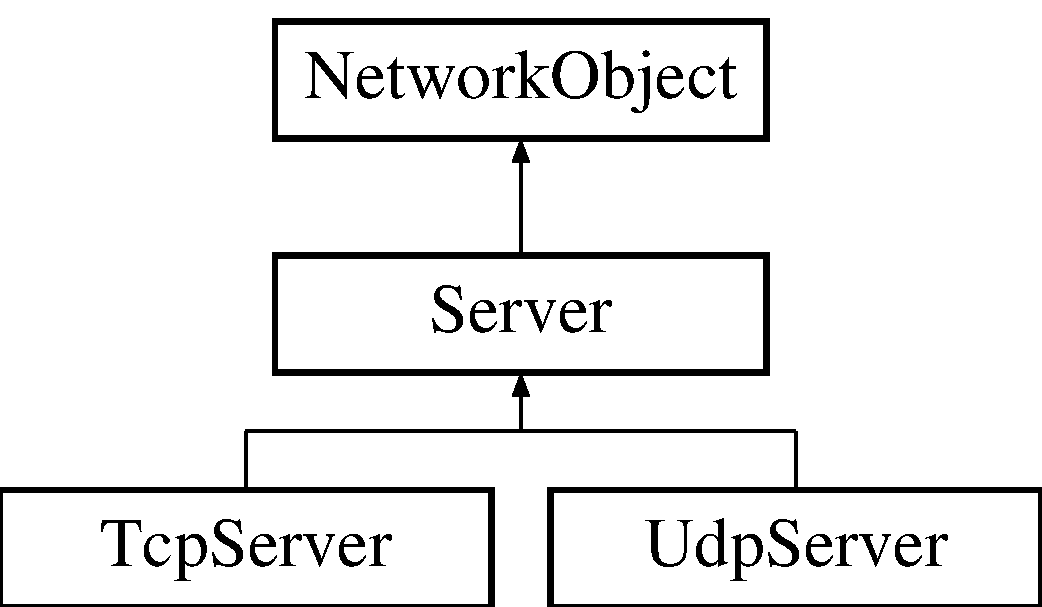
\includegraphics[height=3.000000cm]{classServer}
\end{center}
\end{figure}
\subsection*{Public Member Functions}
\begin{DoxyCompactItemize}
\item 
\hyperlink{classServer_ad5ec9462b520e59f7ea831e157ee5e59}{Server} ()
\item 
virtual \hyperlink{classServer_a263268c249dbe6f49627fd50d496a37f}{$\sim$Server} ()
\item 
virtual void \hyperlink{classServer_ab60269481230955b94dc6405162794b0}{start\_\-listening} ()=0
\item 
virtual int \hyperlink{classServer_abd497ca7e7dc29f8ea4c6ce204839a6d}{get\_\-port} ()=0
\item 
\hyperlink{classServer_a1f501aef583a26270ba174202c7f24e5}{FB\_\-JSAPI\_\-EVENT} (open, 0,())
\end{DoxyCompactItemize}


\subsection{Detailed Description}
An abstract interface for a server object. This registers the generic server-\/specific events to javascript, and registers the 'start\_\-listening' method to the javascript API. 

Definition at line 17 of file Server.h.



\subsection{Constructor \& Destructor Documentation}
\hypertarget{classServer_ad5ec9462b520e59f7ea831e157ee5e59}{
\index{Server@{Server}!Server@{Server}}
\index{Server@{Server}!Server@{Server}}
\subsubsection[{Server}]{\setlength{\rightskip}{0pt plus 5cm}Server::Server (
\begin{DoxyParamCaption}
{}
\end{DoxyParamCaption}
)}}
\label{classServer_ad5ec9462b520e59f7ea831e157ee5e59}
Default constructor for a server object, which registers the 'start\_\-listening' function to the javascript API. 

Definition at line 10 of file Server.cpp.



References get\_\-port(), and start\_\-listening().


\begin{DoxyCode}
{
    registerMethod("listen", make_method(this, &Server::start_listening));
    registerMethod("getPort", make_method(this, &Server::get_port));
}
\end{DoxyCode}
\hypertarget{classServer_a263268c249dbe6f49627fd50d496a37f}{
\index{Server@{Server}!$\sim$Server@{$\sim$Server}}
\index{$\sim$Server@{$\sim$Server}!Server@{Server}}
\subsubsection[{$\sim$Server}]{\setlength{\rightskip}{0pt plus 5cm}virtual Server::$\sim$Server (
\begin{DoxyParamCaption}
{}
\end{DoxyParamCaption}
)\hspace{0.3cm}{\ttfamily  \mbox{[}inline, virtual\mbox{]}}}}
\label{classServer_a263268c249dbe6f49627fd50d496a37f}
Deconstructs a server object 

Definition at line 29 of file Server.h.


\begin{DoxyCode}
{}
\end{DoxyCode}


\subsection{Member Function Documentation}
\hypertarget{classServer_a1f501aef583a26270ba174202c7f24e5}{
\index{Server@{Server}!FB\_\-JSAPI\_\-EVENT@{FB\_\-JSAPI\_\-EVENT}}
\index{FB\_\-JSAPI\_\-EVENT@{FB\_\-JSAPI\_\-EVENT}!Server@{Server}}
\subsubsection[{FB\_\-JSAPI\_\-EVENT}]{\setlength{\rightskip}{0pt plus 5cm}Server::FB\_\-JSAPI\_\-EVENT (
\begin{DoxyParamCaption}
\item[{open}]{, }
\item[{0}]{, }
\item[{()}]{}
\end{DoxyParamCaption}
)}}
\label{classServer_a1f501aef583a26270ba174202c7f24e5}
A javascript event to be fired when the server has started listening for incoming connections successfully. \hypertarget{classServer_abd497ca7e7dc29f8ea4c6ce204839a6d}{
\index{Server@{Server}!get\_\-port@{get\_\-port}}
\index{get\_\-port@{get\_\-port}!Server@{Server}}
\subsubsection[{get\_\-port}]{\setlength{\rightskip}{0pt plus 5cm}virtual int Server::get\_\-port (
\begin{DoxyParamCaption}
{}
\end{DoxyParamCaption}
)\hspace{0.3cm}{\ttfamily  \mbox{[}pure virtual\mbox{]}}}}
\label{classServer_abd497ca7e7dc29f8ea4c6ce204839a6d}
Returns the port on which this server listens 

Implemented in \hyperlink{classTcpServer_a65be01f9466447530de3112d538267b4}{TcpServer}, and \hyperlink{classUdpServer_a276c64a7545b49b298ca3d9ca1a12e9d}{UdpServer}.



Referenced by Server().

\hypertarget{classServer_ab60269481230955b94dc6405162794b0}{
\index{Server@{Server}!start\_\-listening@{start\_\-listening}}
\index{start\_\-listening@{start\_\-listening}!Server@{Server}}
\subsubsection[{start\_\-listening}]{\setlength{\rightskip}{0pt plus 5cm}virtual void Server::start\_\-listening (
\begin{DoxyParamCaption}
{}
\end{DoxyParamCaption}
)\hspace{0.3cm}{\ttfamily  \mbox{[}pure virtual\mbox{]}}}}
\label{classServer_ab60269481230955b94dc6405162794b0}
Called to start the the server listening for the first time, fires the 'open' event, and is exposed to the javascript. This should only be called once, and starts the server listening for incoming connections. 

Implemented in \hyperlink{classTcpServer_ad16f797335dd9c54eaec93c35d158569}{TcpServer}, and \hyperlink{classUdpServer_a55e557d344720286fdeb430ae3cb3842}{UdpServer}.



Referenced by Server().



The documentation for this class was generated from the following files:\begin{DoxyCompactItemize}
\item 
/home/jtedesco/dev/sockit/src/common/\hyperlink{Server_8h}{Server.h}\item 
/home/jtedesco/dev/sockit/src/common/\hyperlink{Server_8cpp}{Server.cpp}\end{DoxyCompactItemize}

\hypertarget{classSockIt}{
\section{SockIt Class Reference}
\label{classSockIt}\index{SockIt@{SockIt}}
}


{\ttfamily \#include $<$SockIt.h$>$}

\subsection*{Public Member Functions}
\begin{DoxyCompactItemize}
\item 
\hyperlink{classSockIt_a6ca1ecc74ae75bff556469cbaca25338}{SockIt} ()
\begin{DoxyCompactList}\small\item\em \hyperlink{classSockIt}{SockIt} constructor. At this point, the API is not yet available, nor is the window. \item\end{DoxyCompactList}\item 
virtual \hyperlink{classSockIt_abcd992a7c2848219c90f29241573a888}{$\sim$SockIt} ()
\begin{DoxyCompactList}\small\item\em \hyperlink{classSockIt}{SockIt} destructor. \item\end{DoxyCompactList}\item 
void \hyperlink{classSockIt_a0ea0da80aff982c421b9dbfa6defc31c}{onPluginReady} ()
\item 
void \hyperlink{classSockIt_af0500187342aa036ba2e9523519f1bed}{shutdown} ()
\item 
virtual FB::JSAPIPtr \hyperlink{classSockIt_a57db1748067287ab0bbc7a096aea8b0b}{createJSAPI} ()
\begin{DoxyCompactList}\small\item\em Creates an instance of the JSAPI object that provides the primary Javascript interface. \item\end{DoxyCompactList}\item 
virtual bool \hyperlink{classSockIt_ad8d0e6627e76f817962f6ec902d86a7e}{isWindowless} ()
\item 
virtual bool \hyperlink{classSockIt_a2224da519bcf7a29c6c26f06c3c830d9}{onMouseDown} (FB::MouseDownEvent $\ast$evt, FB::PluginWindow $\ast$)
\item 
virtual bool \hyperlink{classSockIt_acadbe6be131043cbbcfdc70a672d08d6}{onMouseUp} (FB::MouseUpEvent $\ast$evt, FB::PluginWindow $\ast$)
\item 
virtual bool \hyperlink{classSockIt_aaf869ea6c09a62ecb56ad945ac12e798}{onMouseMove} (FB::MouseMoveEvent $\ast$evt, FB::PluginWindow $\ast$)
\item 
virtual bool \hyperlink{classSockIt_a0334a13dbb896d947679f3fb5e85e347}{onWindowAttached} (FB::AttachedEvent $\ast$evt, FB::PluginWindow $\ast$)
\item 
virtual bool \hyperlink{classSockIt_a87f4e33d21c1dd771b93b3fa595c13d1}{onWindowDetached} (FB::DetachedEvent $\ast$evt, FB::PluginWindow $\ast$)
\end{DoxyCompactItemize}
\subsection*{Static Public Member Functions}
\begin{DoxyCompactItemize}
\item 
static void \hyperlink{classSockIt_aacb050757690c90382b5928fb9d40a76}{StaticInitialize} ()
\begin{DoxyCompactList}\small\item\em Called from \hyperlink{classPluginFactory_a2cc350403d03ea722c910ad11c38e6ec}{PluginFactory::globalPluginInitialize()} \item\end{DoxyCompactList}\item 
static void \hyperlink{classSockIt_a215d0f35f52a6e4c81af37a9938beb64}{StaticDeinitialize} ()
\begin{DoxyCompactList}\small\item\em Called from \hyperlink{classPluginFactory_ab389d98485b8c205afb8e32a07046a52}{PluginFactory::globalPluginDeinitialize()} \item\end{DoxyCompactList}\end{DoxyCompactItemize}


\subsection{Detailed Description}
The root plugin object, auto-\/generated by FireBreath.

\begin{DoxySeeAlso}{See also}
\href{http://www.firebreath.org/}{\tt http://www.firebreath.org/} 
\end{DoxySeeAlso}


Definition at line 25 of file SockIt.h.



\subsection{Constructor \& Destructor Documentation}
\hypertarget{classSockIt_a6ca1ecc74ae75bff556469cbaca25338}{
\index{SockIt@{SockIt}!SockIt@{SockIt}}
\index{SockIt@{SockIt}!SockIt@{SockIt}}
\subsubsection[{SockIt}]{\setlength{\rightskip}{0pt plus 5cm}SockIt::SockIt (
\begin{DoxyParamCaption}
{}
\end{DoxyParamCaption}
)}}
\label{classSockIt_a6ca1ecc74ae75bff556469cbaca25338}


\hyperlink{classSockIt}{SockIt} constructor. At this point, the API is not yet available, nor is the window. 



Definition at line 24 of file SockIt.cpp.


\begin{DoxyCode}
{
}
\end{DoxyCode}
\hypertarget{classSockIt_abcd992a7c2848219c90f29241573a888}{
\index{SockIt@{SockIt}!$\sim$SockIt@{$\sim$SockIt}}
\index{$\sim$SockIt@{$\sim$SockIt}!SockIt@{SockIt}}
\subsubsection[{$\sim$SockIt}]{\setlength{\rightskip}{0pt plus 5cm}SockIt::$\sim$SockIt (
\begin{DoxyParamCaption}
{}
\end{DoxyParamCaption}
)\hspace{0.3cm}{\ttfamily  \mbox{[}virtual\mbox{]}}}}
\label{classSockIt_abcd992a7c2848219c90f29241573a888}


\hyperlink{classSockIt}{SockIt} destructor. 

Tell the host to free the retained JSAPI objects unless the root JSAPI object is referenced somewhere else, it will be released here. 

Definition at line 28 of file SockIt.cpp.


\begin{DoxyCode}
{
    releaseRootJSAPI();
    m_host->freeRetainedObjects();
}
\end{DoxyCode}


\subsection{Member Function Documentation}
\hypertarget{classSockIt_a57db1748067287ab0bbc7a096aea8b0b}{
\index{SockIt@{SockIt}!createJSAPI@{createJSAPI}}
\index{createJSAPI@{createJSAPI}!SockIt@{SockIt}}
\subsubsection[{createJSAPI}]{\setlength{\rightskip}{0pt plus 5cm}FB::JSAPIPtr SockIt::createJSAPI (
\begin{DoxyParamCaption}
{}
\end{DoxyParamCaption}
)\hspace{0.3cm}{\ttfamily  \mbox{[}virtual\mbox{]}}}}
\label{classSockIt_a57db1748067287ab0bbc7a096aea8b0b}


Creates an instance of the JSAPI object that provides the primary Javascript interface. 



Definition at line 43 of file SockIt.cpp.


\begin{DoxyCode}
{
    return boost::make_shared<SockItAPI>(FB::ptr_cast<SockIt>(shared_from_this())
      , m_host);
}
\end{DoxyCode}
\hypertarget{classSockIt_ad8d0e6627e76f817962f6ec902d86a7e}{
\index{SockIt@{SockIt}!isWindowless@{isWindowless}}
\index{isWindowless@{isWindowless}!SockIt@{SockIt}}
\subsubsection[{isWindowless}]{\setlength{\rightskip}{0pt plus 5cm}virtual bool SockIt::isWindowless (
\begin{DoxyParamCaption}
{}
\end{DoxyParamCaption}
)\hspace{0.3cm}{\ttfamily  \mbox{[}inline, virtual\mbox{]}}}}
\label{classSockIt_ad8d0e6627e76f817962f6ec902d86a7e}
Tells the browser whether or not this plugin should have a window associated with it. 

Definition at line 86 of file SockIt.h.


\begin{DoxyCode}
        {
            return false;
        }
\end{DoxyCode}
\hypertarget{classSockIt_a2224da519bcf7a29c6c26f06c3c830d9}{
\index{SockIt@{SockIt}!onMouseDown@{onMouseDown}}
\index{onMouseDown@{onMouseDown}!SockIt@{SockIt}}
\subsubsection[{onMouseDown}]{\setlength{\rightskip}{0pt plus 5cm}bool SockIt::onMouseDown (
\begin{DoxyParamCaption}
\item[{FB::MouseDownEvent $\ast$}]{evt, }
\item[{FB::PluginWindow $\ast$}]{}
\end{DoxyParamCaption}
)\hspace{0.3cm}{\ttfamily  \mbox{[}virtual\mbox{]}}}}
\label{classSockIt_a2224da519bcf7a29c6c26f06c3c830d9}
BEGIN EVENTDEF -\/-\/ DON'T CHANGE THIS LINE 

Definition at line 48 of file SockIt.cpp.


\begin{DoxyCode}
{
    //printf("Mouse down at: %d, %d\n", evt->m_x, evt->m_y);
    return false;
}
\end{DoxyCode}
\hypertarget{classSockIt_aaf869ea6c09a62ecb56ad945ac12e798}{
\index{SockIt@{SockIt}!onMouseMove@{onMouseMove}}
\index{onMouseMove@{onMouseMove}!SockIt@{SockIt}}
\subsubsection[{onMouseMove}]{\setlength{\rightskip}{0pt plus 5cm}bool SockIt::onMouseMove (
\begin{DoxyParamCaption}
\item[{FB::MouseMoveEvent $\ast$}]{evt, }
\item[{FB::PluginWindow $\ast$}]{}
\end{DoxyParamCaption}
)\hspace{0.3cm}{\ttfamily  \mbox{[}virtual\mbox{]}}}}
\label{classSockIt_aaf869ea6c09a62ecb56ad945ac12e798}


Definition at line 60 of file SockIt.cpp.


\begin{DoxyCode}
{
    //printf("Mouse move at: %d, %d\n", evt->m_x, evt->m_y);
    return false;
}
\end{DoxyCode}
\hypertarget{classSockIt_acadbe6be131043cbbcfdc70a672d08d6}{
\index{SockIt@{SockIt}!onMouseUp@{onMouseUp}}
\index{onMouseUp@{onMouseUp}!SockIt@{SockIt}}
\subsubsection[{onMouseUp}]{\setlength{\rightskip}{0pt plus 5cm}bool SockIt::onMouseUp (
\begin{DoxyParamCaption}
\item[{FB::MouseUpEvent $\ast$}]{evt, }
\item[{FB::PluginWindow $\ast$}]{}
\end{DoxyParamCaption}
)\hspace{0.3cm}{\ttfamily  \mbox{[}virtual\mbox{]}}}}
\label{classSockIt_acadbe6be131043cbbcfdc70a672d08d6}


Definition at line 54 of file SockIt.cpp.


\begin{DoxyCode}
{
    //printf("Mouse up at: %d, %d\n", evt->m_x, evt->m_y);
    return false;
}
\end{DoxyCode}
\hypertarget{classSockIt_a0ea0da80aff982c421b9dbfa6defc31c}{
\index{SockIt@{SockIt}!onPluginReady@{onPluginReady}}
\index{onPluginReady@{onPluginReady}!SockIt@{SockIt}}
\subsubsection[{onPluginReady}]{\setlength{\rightskip}{0pt plus 5cm}void SockIt::onPluginReady (
\begin{DoxyParamCaption}
{}
\end{DoxyParamCaption}
)}}
\label{classSockIt_a0ea0da80aff982c421b9dbfa6defc31c}
When this is called, the BrowserHost is attached, the JSAPI object is created, and we are ready to interact with the page and such. The PluginWindow may or may not have already fire the AttachedEvent at this point. 

Definition at line 34 of file SockIt.cpp.


\begin{DoxyCode}
{
}
\end{DoxyCode}
\hypertarget{classSockIt_a0334a13dbb896d947679f3fb5e85e347}{
\index{SockIt@{SockIt}!onWindowAttached@{onWindowAttached}}
\index{onWindowAttached@{onWindowAttached}!SockIt@{SockIt}}
\subsubsection[{onWindowAttached}]{\setlength{\rightskip}{0pt plus 5cm}bool SockIt::onWindowAttached (
\begin{DoxyParamCaption}
\item[{FB::AttachedEvent $\ast$}]{evt, }
\item[{FB::PluginWindow $\ast$}]{}
\end{DoxyParamCaption}
)\hspace{0.3cm}{\ttfamily  \mbox{[}virtual\mbox{]}}}}
\label{classSockIt_a0334a13dbb896d947679f3fb5e85e347}


Definition at line 65 of file SockIt.cpp.


\begin{DoxyCode}
{
    // The window is attached; act appropriately
    return false;
}
\end{DoxyCode}
\hypertarget{classSockIt_a87f4e33d21c1dd771b93b3fa595c13d1}{
\index{SockIt@{SockIt}!onWindowDetached@{onWindowDetached}}
\index{onWindowDetached@{onWindowDetached}!SockIt@{SockIt}}
\subsubsection[{onWindowDetached}]{\setlength{\rightskip}{0pt plus 5cm}bool SockIt::onWindowDetached (
\begin{DoxyParamCaption}
\item[{FB::DetachedEvent $\ast$}]{evt, }
\item[{FB::PluginWindow $\ast$}]{}
\end{DoxyParamCaption}
)\hspace{0.3cm}{\ttfamily  \mbox{[}virtual\mbox{]}}}}
\label{classSockIt_a87f4e33d21c1dd771b93b3fa595c13d1}


Definition at line 71 of file SockIt.cpp.


\begin{DoxyCode}
{
    // The window is about to be detached; act appropriately
    return false;
}
\end{DoxyCode}
\hypertarget{classSockIt_af0500187342aa036ba2e9523519f1bed}{
\index{SockIt@{SockIt}!shutdown@{shutdown}}
\index{shutdown@{shutdown}!SockIt@{SockIt}}
\subsubsection[{shutdown}]{\setlength{\rightskip}{0pt plus 5cm}void SockIt::shutdown (
\begin{DoxyParamCaption}
{}
\end{DoxyParamCaption}
)}}
\label{classSockIt_af0500187342aa036ba2e9523519f1bed}
This will be called when it is time for the plugin to shut down; any threads or anything else that may hold a shared\_\-ptr to this object should be released here so that this object can be safely destroyed. This is the last point that shared\_\-from\_\-this and weak\_\-ptr references to this object will be valid. 

Definition at line 38 of file SockIt.cpp.



Referenced by StaticDeinitialize().


\begin{DoxyCode}
{
}
\end{DoxyCode}
\hypertarget{classSockIt_a215d0f35f52a6e4c81af37a9938beb64}{
\index{SockIt@{SockIt}!StaticDeinitialize@{StaticDeinitialize}}
\index{StaticDeinitialize@{StaticDeinitialize}!SockIt@{SockIt}}
\subsubsection[{StaticDeinitialize}]{\setlength{\rightskip}{0pt plus 5cm}SockIt::StaticDeinitialize (
\begin{DoxyParamCaption}
{}
\end{DoxyParamCaption}
)\hspace{0.3cm}{\ttfamily  \mbox{[}static\mbox{]}}}}
\label{classSockIt_a215d0f35f52a6e4c81af37a9938beb64}


Called from \hyperlink{classPluginFactory_ab389d98485b8c205afb8e32a07046a52}{PluginFactory::globalPluginDeinitialize()} 

Performs one-\/time global de-\/initialization of the plugin. This should be called just before the plugin library is unloaded

\begin{DoxySeeAlso}{See also}
FB::FactoryBase::globalPluginDeinitialize 
\end{DoxySeeAlso}


Definition at line 19 of file SockIt.cpp.



References shutdown().



Referenced by PluginFactory::globalPluginDeinitialize().


\begin{DoxyCode}
{
    Logger::shutdown();
}
\end{DoxyCode}
\hypertarget{classSockIt_aacb050757690c90382b5928fb9d40a76}{
\index{SockIt@{SockIt}!StaticInitialize@{StaticInitialize}}
\index{StaticInitialize@{StaticInitialize}!SockIt@{SockIt}}
\subsubsection[{StaticInitialize}]{\setlength{\rightskip}{0pt plus 5cm}SockIt::StaticInitialize (
\begin{DoxyParamCaption}
{}
\end{DoxyParamCaption}
)\hspace{0.3cm}{\ttfamily  \mbox{[}static\mbox{]}}}}
\label{classSockIt_aacb050757690c90382b5928fb9d40a76}


Called from \hyperlink{classPluginFactory_a2cc350403d03ea722c910ad11c38e6ec}{PluginFactory::globalPluginInitialize()} 

Performs one-\/time global initialization of the plugin. This should only be called once per process.

\begin{DoxySeeAlso}{See also}
FB::FactoryBase::globalPluginInitialize 
\end{DoxySeeAlso}


Definition at line 14 of file SockIt.cpp.



Referenced by PluginFactory::globalPluginInitialize().


\begin{DoxyCode}
{
    // add any library initialization routines here
}
\end{DoxyCode}


The documentation for this class was generated from the following files:\begin{DoxyCompactItemize}
\item 
/home/jtedesco/dev/sockit/src/plugin/\hyperlink{SockIt_8h}{SockIt.h}\item 
/home/jtedesco/dev/sockit/src/plugin/\hyperlink{SockIt_8cpp}{SockIt.cpp}\end{DoxyCompactItemize}

\hypertarget{classSockItAPI}{
\section{SockItAPI Class Reference}
\label{classSockItAPI}\index{SockItAPI@{SockItAPI}}
}


{\ttfamily \#include $<$SockItAPI.h$>$}

\subsection*{Public Member Functions}
\begin{DoxyCompactItemize}
\item 
\hyperlink{classSockItAPI_abe90f8a1c172737a1c52d7216b0adee1}{SockItAPI} (const SockItPtr \&plugin, const FB::BrowserHostPtr \&host)
\item 
virtual \hyperlink{classSockItAPI_ab1bdcadeb41aea91e9adb5ae934bf742}{$\sim$SockItAPI} ()
\begin{DoxyCompactList}\small\item\em Destructor. Remember that this object will not be released until the browser is done with it; this will almost definitely be after the plugin is released. \item\end{DoxyCompactList}\item 
SockItPtr \hyperlink{classSockItAPI_a196d7874f3124a28bca5dd3f9acb5c60}{getPlugin} ()
\begin{DoxyCompactList}\small\item\em Gets a reference to the plugin that was passed in when the object was created. If the plugin has already been released then this will throw a FB::script\_\-error that will be translated into a javascript exception in the page. \item\end{DoxyCompactList}\item 
boost::shared\_\-ptr$<$ \hyperlink{classNetworkThread}{NetworkThread} $>$ \hyperlink{classSockItAPI_a5de4cedcdcfff3bc3fd88aa52f62b2eb}{create\_\-thread} ()
\item 
boost::shared\_\-ptr$<$ \hyperlink{classTcpServer}{TcpServer} $>$ \hyperlink{classSockItAPI_a48b4b81ac34fb4135c2067eb5477144a}{create\_\-tcp\_\-server} (int port, boost::optional$<$ map$<$ string, string $>$ $>$ options)
\item 
boost::shared\_\-ptr$<$ \hyperlink{classTcpClient}{TcpClient} $>$ \hyperlink{classSockItAPI_a926d3fe9cdbcf52f4a40a922a4d3a0b7}{create\_\-tcp\_\-client} (const string \&host, int port, boost::optional$<$ map$<$ string, string $>$ $>$ options)
\item 
boost::shared\_\-ptr$<$ \hyperlink{classUdpServer}{UdpServer} $>$ \hyperlink{classSockItAPI_afede6ca76e58e088b3262b02bb47d1a0}{create\_\-udp\_\-server} (int port, boost::optional$<$ map$<$ string, string $>$ $>$ options)
\item 
boost::shared\_\-ptr$<$ \hyperlink{classUdpClient}{UdpClient} $>$ \hyperlink{classSockItAPI_a459c942a85f434e96dec5cdff753ed3a}{create\_\-udp\_\-client} (const string \&host, int port, boost::optional$<$ map$<$ string, string $>$ $>$ options)
\item 
\hyperlink{Event_8h_a42e68af8ed186972f3b40e079e28dfb1}{binary} \hyperlink{classSockItAPI_a5eac49bd5ad0cb5320cbc325a0e997be}{convert\_\-to\_\-binary} (const vector$<$ \hyperlink{Event_8h_ae0aa21f6bcb621fe36c2c962aa0452fe}{byte} $>$ bytes)
\item 
FB::VariantList \hyperlink{classSockItAPI_a4e507273c91d6509be9133a34c32ed3c}{convert\_\-from\_\-binary} (\hyperlink{Event_8h_a42e68af8ed186972f3b40e079e28dfb1}{binary} data)
\end{DoxyCompactItemize}
\subsection*{Private Attributes}
\begin{DoxyCompactItemize}
\item 
\hyperlink{classNetworkThread}{NetworkThread} \hyperlink{classSockItAPI_adcfb54795f58d245c1b8ea8311a7d456}{default\_\-thread}
\item 
SockItWeakPtr \hyperlink{classSockItAPI_ac973fa980fa71d06190969448621beea}{m\_\-plugin}
\item 
FB::BrowserHostPtr \hyperlink{classSockItAPI_afb9c76de5331308b066e969d9a35d236}{m\_\-host}
\end{DoxyCompactItemize}


\subsection{Detailed Description}
Exposes the plugin's API to the browser. Primarily auto-\/generated by FireBreath, but edited to add root methods for the plugin and expose them to the javascript.

\begin{DoxySeeAlso}{See also}
\href{http://www.firebreath.org/}{\tt http://www.firebreath.org/} 
\end{DoxySeeAlso}


Definition at line 35 of file SockItAPI.h.



\subsection{Constructor \& Destructor Documentation}
\hypertarget{classSockItAPI_abe90f8a1c172737a1c52d7216b0adee1}{
\index{SockItAPI@{SockItAPI}!SockItAPI@{SockItAPI}}
\index{SockItAPI@{SockItAPI}!SockItAPI@{SockItAPI}}
\subsubsection[{SockItAPI}]{\setlength{\rightskip}{0pt plus 5cm}SockItAPI::SockItAPI (
\begin{DoxyParamCaption}
\item[{const SockItPtr \&}]{plugin, }
\item[{const FB::BrowserHostPtr \&}]{host}
\end{DoxyParamCaption}
)}}
\label{classSockItAPI_abe90f8a1c172737a1c52d7216b0adee1}
Constructor for the JSAPI object. Registers root API methods for the plugin to be available to Javascript.

\begin{DoxySeeAlso}{See also}
FB::JSAPIAuto::registerMethod 

FB::JSAPIAuto::registerProperty 

FB::JSAPIAuto::registerEvent 
\end{DoxySeeAlso}


Definition at line 12 of file SockItAPI.cpp.



References convert\_\-from\_\-binary(), convert\_\-to\_\-binary(), create\_\-tcp\_\-client(), create\_\-tcp\_\-server(), create\_\-thread(), create\_\-udp\_\-client(), and create\_\-udp\_\-server().


\begin{DoxyCode}
                                                                          :
    m_plugin(plugin), m_host(host)
{
    // Register root methods for creating network threads
    registerMethod("createThread", make_method(this, &SockItAPI::create_thread));
      

    // Register root methods for creating servers & clients
    registerMethod("createUdpClient", make_method(this, &
      SockItAPI::create_udp_client));
    registerMethod("createUdpServer", make_method(this, &
      SockItAPI::create_udp_server));
    registerMethod("createTcpClient", make_method(this, &
      SockItAPI::create_tcp_client));
    registerMethod("createTcpServer", make_method(this, &
      SockItAPI::create_tcp_server));

    // Register methods for converting to and from binary data
    registerMethod("toBinary", make_method(this, &SockItAPI::convert_to_binary));
      
    registerMethod("fromBinary", make_method(this, &
      SockItAPI::convert_from_binary));
}
\end{DoxyCode}
\hypertarget{classSockItAPI_ab1bdcadeb41aea91e9adb5ae934bf742}{
\index{SockItAPI@{SockItAPI}!$\sim$SockItAPI@{$\sim$SockItAPI}}
\index{$\sim$SockItAPI@{$\sim$SockItAPI}!SockItAPI@{SockItAPI}}
\subsubsection[{$\sim$SockItAPI}]{\setlength{\rightskip}{0pt plus 5cm}SockItAPI::$\sim$SockItAPI (
\begin{DoxyParamCaption}
{}
\end{DoxyParamCaption}
)\hspace{0.3cm}{\ttfamily  \mbox{[}virtual\mbox{]}}}}
\label{classSockItAPI_ab1bdcadeb41aea91e9adb5ae934bf742}


Destructor. Remember that this object will not be released until the browser is done with it; this will almost definitely be after the plugin is released. 



Definition at line 29 of file SockItAPI.cpp.


\begin{DoxyCode}
{
}
\end{DoxyCode}


\subsection{Member Function Documentation}
\hypertarget{classSockItAPI_a4e507273c91d6509be9133a34c32ed3c}{
\index{SockItAPI@{SockItAPI}!convert\_\-from\_\-binary@{convert\_\-from\_\-binary}}
\index{convert\_\-from\_\-binary@{convert\_\-from\_\-binary}!SockItAPI@{SockItAPI}}
\subsubsection[{convert\_\-from\_\-binary}]{\setlength{\rightskip}{0pt plus 5cm}FB::VariantList SockItAPI::convert\_\-from\_\-binary (
\begin{DoxyParamCaption}
\item[{{\bf binary}}]{data}
\end{DoxyParamCaption}
)}}
\label{classSockItAPI_a4e507273c91d6509be9133a34c32ed3c}
Utility function for converting a string, assumed to be binary data returned from {\ttfamily convert\_\-to\_\-binary}.


\begin{DoxyParams}{Parameters}
{\em data} & The (binary) data to be converted to an array of characters \\
\hline
\end{DoxyParams}


Definition at line 83 of file SockItAPI.cpp.



Referenced by SockItAPI().


\begin{DoxyCode}
{
    vector<byte> bytes;
    for(int i = 0; i < data.size(); i++)
    {
        bytes.push_back((unsigned char) data.data()[i]);
    }

    FB::VariantList fb_bytes;
    std::copy(bytes.begin(), bytes.end(), std::back_inserter(fb_bytes));
    return fb_bytes;
}
\end{DoxyCode}
\hypertarget{classSockItAPI_a5eac49bd5ad0cb5320cbc325a0e997be}{
\index{SockItAPI@{SockItAPI}!convert\_\-to\_\-binary@{convert\_\-to\_\-binary}}
\index{convert\_\-to\_\-binary@{convert\_\-to\_\-binary}!SockItAPI@{SockItAPI}}
\subsubsection[{convert\_\-to\_\-binary}]{\setlength{\rightskip}{0pt plus 5cm}{\bf binary} SockItAPI::convert\_\-to\_\-binary (
\begin{DoxyParamCaption}
\item[{const vector$<$ {\bf byte} $>$}]{bytes}
\end{DoxyParamCaption}
)}}
\label{classSockItAPI_a5eac49bd5ad0cb5320cbc325a0e997be}
Utility function for converting an array of integers, assumed to hexadecimal numbers, to a string.


\begin{DoxyParams}{Parameters}
{\em bytes} & The bytes of data to be converted into a string \\
\hline
\end{DoxyParams}


Definition at line 70 of file SockItAPI.cpp.



Referenced by SockItAPI().


\begin{DoxyCode}
{
    // Convert it to a character array and create a string from it
    binary data;

    for (int i = 0; i < bytes.size(); i++)
    {
        data.push_back((unsigned char) bytes[i]);
    }

    return data;
}
\end{DoxyCode}
\hypertarget{classSockItAPI_a926d3fe9cdbcf52f4a40a922a4d3a0b7}{
\index{SockItAPI@{SockItAPI}!create\_\-tcp\_\-client@{create\_\-tcp\_\-client}}
\index{create\_\-tcp\_\-client@{create\_\-tcp\_\-client}!SockItAPI@{SockItAPI}}
\subsubsection[{create\_\-tcp\_\-client}]{\setlength{\rightskip}{0pt plus 5cm}boost::shared\_\-ptr$<$ {\bf TcpClient} $>$ SockItAPI::create\_\-tcp\_\-client (
\begin{DoxyParamCaption}
\item[{const string \&}]{host, }
\item[{int}]{port, }
\item[{boost::optional$<$ map$<$ string, string $>$ $>$}]{options}
\end{DoxyParamCaption}
)}}
\label{classSockItAPI_a926d3fe9cdbcf52f4a40a922a4d3a0b7}
Creates a new TCP client on the default {\ttfamily \hyperlink{classNetworkThread}{NetworkThread}}.


\begin{DoxyParams}{Parameters}
{\em host} & The hostname to which this TCP client will connect \\
\hline
{\em port} & The port on the remote host to which this client should connect \\
\hline
{\em options} & The set of options passed in from Javascript. \\
\hline
\end{DoxyParams}
\begin{DoxyReturn}{Returns}
A shared pointer to a newly created TCP client 
\end{DoxyReturn}


Definition at line 53 of file SockItAPI.cpp.



References NetworkThread::create\_\-tcp\_\-client(), and default\_\-thread.



Referenced by SockItAPI().


\begin{DoxyCode}
{
    return default_thread.create_tcp_client(host, port, options);
}
\end{DoxyCode}
\hypertarget{classSockItAPI_a48b4b81ac34fb4135c2067eb5477144a}{
\index{SockItAPI@{SockItAPI}!create\_\-tcp\_\-server@{create\_\-tcp\_\-server}}
\index{create\_\-tcp\_\-server@{create\_\-tcp\_\-server}!SockItAPI@{SockItAPI}}
\subsubsection[{create\_\-tcp\_\-server}]{\setlength{\rightskip}{0pt plus 5cm}boost::shared\_\-ptr$<$ {\bf TcpServer} $>$ SockItAPI::create\_\-tcp\_\-server (
\begin{DoxyParamCaption}
\item[{int}]{port, }
\item[{boost::optional$<$ map$<$ string, string $>$ $>$}]{options}
\end{DoxyParamCaption}
)}}
\label{classSockItAPI_a48b4b81ac34fb4135c2067eb5477144a}
Creates a new TCP server on the default {\ttfamily \hyperlink{classNetworkThread}{NetworkThread}}.


\begin{DoxyParams}{Parameters}
{\em port} & The port on which this new TCP server should listen \\
\hline
{\em options} & The set of options passed in from Javascript. \\
\hline
\end{DoxyParams}
\begin{DoxyReturn}{Returns}
A shared pointer to a newly created TCP server 
\end{DoxyReturn}


Definition at line 48 of file SockItAPI.cpp.



References NetworkThread::create\_\-tcp\_\-server(), and default\_\-thread.



Referenced by SockItAPI().


\begin{DoxyCode}
{
    return default_thread.create_tcp_server(port, options);
}
\end{DoxyCode}
\hypertarget{classSockItAPI_a5de4cedcdcfff3bc3fd88aa52f62b2eb}{
\index{SockItAPI@{SockItAPI}!create\_\-thread@{create\_\-thread}}
\index{create\_\-thread@{create\_\-thread}!SockItAPI@{SockItAPI}}
\subsubsection[{create\_\-thread}]{\setlength{\rightskip}{0pt plus 5cm}boost::shared\_\-ptr$<$ {\bf NetworkThread} $>$ SockItAPI::create\_\-thread (
\begin{DoxyParamCaption}
{}
\end{DoxyParamCaption}
)}}
\label{classSockItAPI_a5de4cedcdcfff3bc3fd88aa52f62b2eb}
Creates a new {\ttfamily \hyperlink{classNetworkThread}{NetworkThread}} object on which we can create new clients and servers.

\begin{DoxyReturn}{Returns}
A shared pointer to a newly created {\ttfamily \hyperlink{classNetworkThread}{NetworkThread}} object 
\end{DoxyReturn}


Definition at line 43 of file SockItAPI.cpp.



Referenced by SockItAPI().


\begin{DoxyCode}
{
    return boost::shared_ptr<NetworkThread>(new NetworkThread());
}
\end{DoxyCode}
\hypertarget{classSockItAPI_a459c942a85f434e96dec5cdff753ed3a}{
\index{SockItAPI@{SockItAPI}!create\_\-udp\_\-client@{create\_\-udp\_\-client}}
\index{create\_\-udp\_\-client@{create\_\-udp\_\-client}!SockItAPI@{SockItAPI}}
\subsubsection[{create\_\-udp\_\-client}]{\setlength{\rightskip}{0pt plus 5cm}boost::shared\_\-ptr$<$ {\bf UdpClient} $>$ SockItAPI::create\_\-udp\_\-client (
\begin{DoxyParamCaption}
\item[{const string \&}]{host, }
\item[{int}]{port, }
\item[{boost::optional$<$ map$<$ string, string $>$ $>$}]{options}
\end{DoxyParamCaption}
)}}
\label{classSockItAPI_a459c942a85f434e96dec5cdff753ed3a}
Creates a new UDP client on the default {\ttfamily \hyperlink{classNetworkThread}{NetworkThread}}.


\begin{DoxyParams}{Parameters}
{\em host} & The hostname to which this UDP client will connect \\
\hline
{\em port} & The port on the remote host to which this client should connect \\
\hline
{\em options} & The set of options passed in from Javascript. \\
\hline
\end{DoxyParams}
\begin{DoxyReturn}{Returns}
A shared pointer to a newly created UDP client 
\end{DoxyReturn}


Definition at line 64 of file SockItAPI.cpp.



References NetworkThread::create\_\-udp\_\-client(), and default\_\-thread.



Referenced by SockItAPI().


\begin{DoxyCode}
{
    return default_thread.create_udp_client(host, port, options);
}
\end{DoxyCode}
\hypertarget{classSockItAPI_afede6ca76e58e088b3262b02bb47d1a0}{
\index{SockItAPI@{SockItAPI}!create\_\-udp\_\-server@{create\_\-udp\_\-server}}
\index{create\_\-udp\_\-server@{create\_\-udp\_\-server}!SockItAPI@{SockItAPI}}
\subsubsection[{create\_\-udp\_\-server}]{\setlength{\rightskip}{0pt plus 5cm}boost::shared\_\-ptr$<$ {\bf UdpServer} $>$ SockItAPI::create\_\-udp\_\-server (
\begin{DoxyParamCaption}
\item[{int}]{port, }
\item[{boost::optional$<$ map$<$ string, string $>$ $>$}]{options}
\end{DoxyParamCaption}
)}}
\label{classSockItAPI_afede6ca76e58e088b3262b02bb47d1a0}
Creates a new UDP server on the default {\ttfamily \hyperlink{classNetworkThread}{NetworkThread}}.


\begin{DoxyParams}{Parameters}
{\em port} & The port on which this new UDP server should listen \\
\hline
{\em options} & The set of options passed in from Javascript. \\
\hline
\end{DoxyParams}
\begin{DoxyReturn}{Returns}
A shared pointer to a newly created UDP server 
\end{DoxyReturn}


Definition at line 59 of file SockItAPI.cpp.



References NetworkThread::create\_\-udp\_\-server(), and default\_\-thread.



Referenced by SockItAPI().


\begin{DoxyCode}
{
    return default_thread.create_udp_server(port, options);
}
\end{DoxyCode}
\hypertarget{classSockItAPI_a196d7874f3124a28bca5dd3f9acb5c60}{
\index{SockItAPI@{SockItAPI}!getPlugin@{getPlugin}}
\index{getPlugin@{getPlugin}!SockItAPI@{SockItAPI}}
\subsubsection[{getPlugin}]{\setlength{\rightskip}{0pt plus 5cm}SockItPtr SockItAPI::getPlugin (
\begin{DoxyParamCaption}
{}
\end{DoxyParamCaption}
)}}
\label{classSockItAPI_a196d7874f3124a28bca5dd3f9acb5c60}


Gets a reference to the plugin that was passed in when the object was created. If the plugin has already been released then this will throw a FB::script\_\-error that will be translated into a javascript exception in the page. 



Definition at line 33 of file SockItAPI.cpp.



References m\_\-plugin.


\begin{DoxyCode}
{
    SockItPtr plugin(m_plugin.lock());
    if (!plugin)
    {
        throw FB::script_error("The plugin is invalid");
    }
    return plugin;
}
\end{DoxyCode}


\subsection{Member Data Documentation}
\hypertarget{classSockItAPI_adcfb54795f58d245c1b8ea8311a7d456}{
\index{SockItAPI@{SockItAPI}!default\_\-thread@{default\_\-thread}}
\index{default\_\-thread@{default\_\-thread}!SockItAPI@{SockItAPI}}
\subsubsection[{default\_\-thread}]{\setlength{\rightskip}{0pt plus 5cm}{\bf NetworkThread} {\bf SockItAPI::default\_\-thread}\hspace{0.3cm}{\ttfamily  \mbox{[}private\mbox{]}}}}
\label{classSockItAPI_adcfb54795f58d245c1b8ea8311a7d456}
The default network thread used if no thread is explicitly created. 

Definition at line 127 of file SockItAPI.h.



Referenced by create\_\-tcp\_\-client(), create\_\-tcp\_\-server(), create\_\-udp\_\-client(), and create\_\-udp\_\-server().

\hypertarget{classSockItAPI_afb9c76de5331308b066e969d9a35d236}{
\index{SockItAPI@{SockItAPI}!m\_\-host@{m\_\-host}}
\index{m\_\-host@{m\_\-host}!SockItAPI@{SockItAPI}}
\subsubsection[{m\_\-host}]{\setlength{\rightskip}{0pt plus 5cm}FB::BrowserHostPtr {\bf SockItAPI::m\_\-host}\hspace{0.3cm}{\ttfamily  \mbox{[}private\mbox{]}}}}
\label{classSockItAPI_afb9c76de5331308b066e969d9a35d236}
A handle on the browser to gather information if necessary. 

Definition at line 137 of file SockItAPI.h.

\hypertarget{classSockItAPI_ac973fa980fa71d06190969448621beea}{
\index{SockItAPI@{SockItAPI}!m\_\-plugin@{m\_\-plugin}}
\index{m\_\-plugin@{m\_\-plugin}!SockItAPI@{SockItAPI}}
\subsubsection[{m\_\-plugin}]{\setlength{\rightskip}{0pt plus 5cm}SockItWeakPtr {\bf SockItAPI::m\_\-plugin}\hspace{0.3cm}{\ttfamily  \mbox{[}private\mbox{]}}}}
\label{classSockItAPI_ac973fa980fa71d06190969448621beea}
A handle on the plugin object itself. 

Definition at line 132 of file SockItAPI.h.



Referenced by getPlugin().



The documentation for this class was generated from the following files:\begin{DoxyCompactItemize}
\item 
/home/jtedesco/dev/sockit/src/plugin/\hyperlink{SockItAPI_8h}{SockItAPI.h}\item 
/home/jtedesco/dev/sockit/src/plugin/\hyperlink{SockItAPI_8cpp}{SockItAPI.cpp}\end{DoxyCompactItemize}

\hypertarget{classTcp}{
\section{Tcp Class Reference}
\label{classTcp}\index{Tcp@{Tcp}}
}


{\ttfamily \#include $<$Tcp.h$>$}

Inheritance diagram for Tcp:\begin{figure}[H]
\begin{center}
\leavevmode
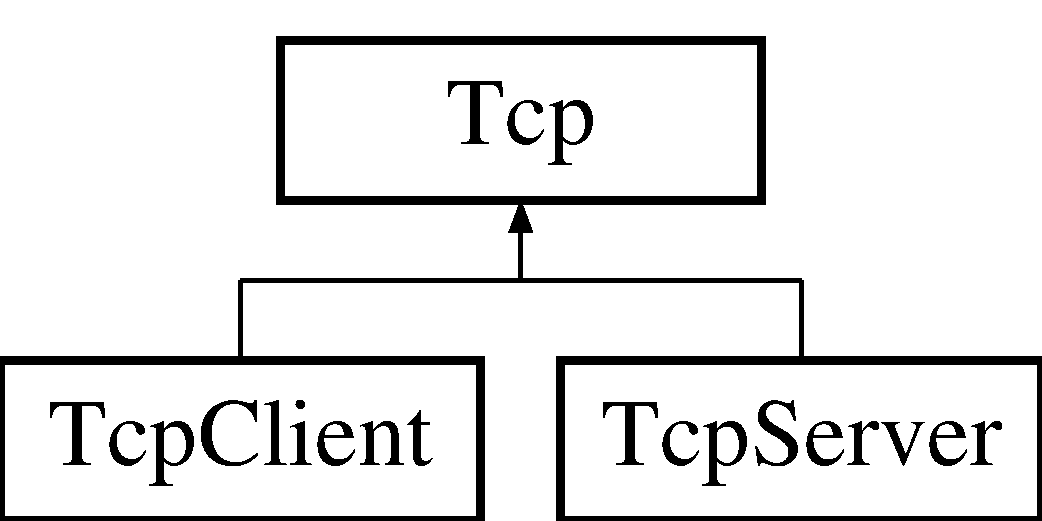
\includegraphics[height=2.000000cm]{classTcp}
\end{center}
\end{figure}
\subsection*{Public Member Functions}
\begin{DoxyCompactItemize}
\item 
\hyperlink{classTcp_af081afa2fd34edc12ac0dda43851352c}{Tcp} (string \hyperlink{classTcp_a0e981d15f94a460b91845bce9b930c61}{host}, int \hyperlink{classTcp_a7ed15f78afc9d0675404b4b41cc723ba}{port}, boost::asio::io\_\-service \&\hyperlink{classTcp_ad0c319a0974aa3f07e9c5ae290ea18b4}{io\_\-service})
\item 
virtual \hyperlink{classTcp_ab5d2bbefce3133529f51b2afa2796b90}{$\sim$Tcp} ()
\end{DoxyCompactItemize}
\subsection*{Protected Member Functions}
\begin{DoxyCompactItemize}
\item 
bool \hyperlink{classTcp_aea9e4a82b08f1893900dad21a1fedfb7}{set\_\-tcp\_\-keepalive} (boost::shared\_\-ptr$<$ tcp::socket $>$ socket)
\item 
string \hyperlink{classTcp_af93fb7459faba8da96f1df55728dfeee}{bool\_\-option\_\-to\_\-string} (optional$<$ bool $>$ \&arg, string iftrue, string iffalse)
\item 
{\footnotesize template$<$class T $>$ }\\string \hyperlink{classTcp_a6324523a33b5830641fd22e32bab8066}{option\_\-to\_\-string} (optional$<$ T $>$ \&arg)
\item 
void \hyperlink{classTcp_a5eae377b9c7c4e49a210a0372bdb9f73}{parse\_\-string\_\-bool\_\-arg} (map$<$ string, string $>$ \&options, string arg, optional$<$ bool $>$ \&arg\_\-value)
\item 
void \hyperlink{classTcp_a91de22f151e40c56638ae54899f1be5a}{parse\_\-string\_\-int\_\-arg} (map$<$ string, string $>$ \&options, string arg, optional$<$ int $>$ \&arg\_\-value)
\item 
void \hyperlink{classTcp_a65753a8c2d9bad07216abdcd5a8a1e86}{parse\_\-args} (map$<$ string, string $>$ options)
\item 
void \hyperlink{classTcp_a59aee046563f221c89ab4b56146fcdc7}{log\_\-options} ()
\item 
virtual void \hyperlink{classTcp_a48b0192669ab99dc953ab3feae5c1b1c}{close} ()=0
\item 
virtual void \hyperlink{classTcp_a447cf3ccc28a073a6b871dd1f597c28d}{send\_\-handler} (const boost::system::error\_\-code \&error\_\-code, std::size\_\-t bytes\_\-transferred, string data, string \hyperlink{classTcp_a0e981d15f94a460b91845bce9b930c61}{host}, int \hyperlink{classTcp_a7ed15f78afc9d0675404b4b41cc723ba}{port}, boost::shared\_\-ptr$<$ tcp::socket $>$ connection)
\item 
virtual void \hyperlink{classTcp_a96707e496b0fcef660c3f22fb6efc0fd}{receive\_\-handler} (const boost::system::error\_\-code \&error\_\-code, std::size\_\-t bytes\_\-transferred, boost::shared\_\-ptr$<$ tcp::socket $>$ connection, string \hyperlink{classTcp_a0e981d15f94a460b91845bce9b930c61}{host}, int \hyperlink{classTcp_a7ed15f78afc9d0675404b4b41cc723ba}{port})
\item 
virtual void \hyperlink{classTcp_a9798750750bc775de9a16d0f148bc002}{fire\_\-error\_\-event} (const string \&message)=0
\item 
virtual void \hyperlink{classTcp_a69d92d55403e877f252bbfbfd7c02ec2}{fire\_\-disconnect\_\-event} (const string \&message)=0
\item 
virtual void \hyperlink{classTcp_a7e5cfd764f04ca5e2729924b9d537db2}{fire\_\-data\_\-event} (const string data, boost::shared\_\-ptr$<$ tcp::socket $>$ connection)=0
\end{DoxyCompactItemize}
\subsection*{Protected Attributes}
\begin{DoxyCompactItemize}
\item 
boost::array$<$ char, \hyperlink{classTcp_a9302fa700d80ca1aed86e41e02925051}{BUFFER\_\-SIZE} $>$ \hyperlink{classTcp_aeb630e95d24f26852437098df5896b16}{receive\_\-buffer}
\item 
boost::asio::io\_\-service \& \hyperlink{classTcp_ad0c319a0974aa3f07e9c5ae290ea18b4}{io\_\-service}
\item 
bool \hyperlink{classTcp_a96b0558a6ce522708bfd06cf1e6e45ba}{waiting\_\-to\_\-shutdown}
\item 
optional$<$ bool $>$ \hyperlink{classTcp_a395b2458742a84d78c1107ac8b59a7a8}{using\_\-ipv6}
\item 
optional$<$ bool $>$ \hyperlink{classTcp_a00a788b6d5b91b31b340f942617b9dda}{no\_\-delay}
\item 
optional$<$ bool $>$ \hyperlink{classTcp_a6bff7fed84126b745930da36030c68c7}{do\_\-not\_\-route}
\item 
optional$<$ bool $>$ \hyperlink{classTcp_a5cec5af76ec94551f8dc5f98639e9953}{keep\_\-alive}
\item 
optional$<$ int $>$ \hyperlink{classTcp_a08e171f501f01c117f5a3c04d394d137}{keep\_\-alive\_\-timeout}
\item 
int \hyperlink{classTcp_a4811b96fe77f74f10b14aac532036708}{active\_\-jobs}
\item 
boost::mutex \hyperlink{classTcp_adcd27ee2753e2c0c43f58efa882a3ab5}{active\_\-jobs\_\-mutex}
\item 
string \hyperlink{classTcp_a0e981d15f94a460b91845bce9b930c61}{host}
\item 
int \hyperlink{classTcp_a7ed15f78afc9d0675404b4b41cc723ba}{port}
\item 
std::set$<$ boost::system::error\_\-code $>$ \hyperlink{classTcp_adcbc3e86d98f8ba37247674cf67f77fd}{disconnect\_\-errors}
\item 
bool \hyperlink{classTcp_a9dbc59f5343aa045be1a888356ef6fbf}{failed}
\end{DoxyCompactItemize}
\subsection*{Static Protected Attributes}
\begin{DoxyCompactItemize}
\item 
static const int \hyperlink{classTcp_a9302fa700d80ca1aed86e41e02925051}{BUFFER\_\-SIZE} = 4096
\item 
static const int \hyperlink{classTcp_a169a3d26315c2b5eecc02354ef44b777}{MAX\_\-DATA\_\-SIZE} = 65536
\end{DoxyCompactItemize}
\subsection*{Friends}
\begin{DoxyCompactItemize}
\item 
class \hyperlink{classTcp_ac01935b5a2bc7cc5ef28348f3d64ffa2}{TcpEvent}
\end{DoxyCompactItemize}


\subsection{Detailed Description}
Interface to abstract out the client-\/server model for use in the {\ttfamily \hyperlink{classEvent}{Event}}. Contains common handlers used by both TCP servers and clients.

\begin{DoxySeeAlso}{See also}
\hyperlink{classEvent}{Event} 
\end{DoxySeeAlso}


Definition at line 60 of file Tcp.h.



\subsection{Constructor \& Destructor Documentation}
\hypertarget{classTcp_af081afa2fd34edc12ac0dda43851352c}{
\index{Tcp@{Tcp}!Tcp@{Tcp}}
\index{Tcp@{Tcp}!Tcp@{Tcp}}
\subsubsection[{Tcp}]{\setlength{\rightskip}{0pt plus 5cm}Tcp::Tcp (
\begin{DoxyParamCaption}
\item[{string}]{host, }
\item[{int}]{port, }
\item[{boost::asio::io\_\-service \&}]{io\_\-service}
\end{DoxyParamCaption}
)}}
\label{classTcp_af081afa2fd34edc12ac0dda43851352c}
Builds a generic TCP object, and registers the 'shutdown' method on the API.


\begin{DoxyParams}{Parameters}
{\em host} & The hostname for this TCP object. For clients, this represents the remote host's hostname, and for servers, defaults to 'localhost'. \\
\hline
{\em port} & The port for this TCP object, which for clients, represents the port of the remote host to which to connect, and for servers, represents the port to which to bind and listen for incoming connections. \\
\hline
{\em io\_\-service} & The I/O service used for asynchronous I/O requests \\
\hline
\end{DoxyParams}


Definition at line 10 of file Tcp.cpp.



References disconnect\_\-errors.


\begin{DoxyCode}
                                                               :
    host(host), port(port), waiting_to_shutdown(false), active_jobs(0), 
      io_service(ioService), using_ipv6(false), failed(false)
{
    // Collect the set of errors classified as 'disconnect' type errors
    disconnect_errors.insert(boost::asio::error::connection_reset);
    disconnect_errors.insert(boost::asio::error::eof);
    disconnect_errors.insert(boost::asio::error::connection_aborted);
    disconnect_errors.insert(boost::asio::error::operation_aborted);
}
\end{DoxyCode}
\hypertarget{classTcp_ab5d2bbefce3133529f51b2afa2796b90}{
\index{Tcp@{Tcp}!$\sim$Tcp@{$\sim$Tcp}}
\index{$\sim$Tcp@{$\sim$Tcp}!Tcp@{Tcp}}
\subsubsection[{$\sim$Tcp}]{\setlength{\rightskip}{0pt plus 5cm}virtual Tcp::$\sim$Tcp (
\begin{DoxyParamCaption}
{}
\end{DoxyParamCaption}
)\hspace{0.3cm}{\ttfamily  \mbox{[}inline, virtual\mbox{]}}}}
\label{classTcp_ab5d2bbefce3133529f51b2afa2796b90}
Immediately calls the {\ttfamily close} function, freeing all resources for this TCP object and shutting down any open connections. 

Definition at line 80 of file Tcp.h.


\begin{DoxyCode}
{}
\end{DoxyCode}


\subsection{Member Function Documentation}
\hypertarget{classTcp_af93fb7459faba8da96f1df55728dfeee}{
\index{Tcp@{Tcp}!bool\_\-option\_\-to\_\-string@{bool\_\-option\_\-to\_\-string}}
\index{bool\_\-option\_\-to\_\-string@{bool\_\-option\_\-to\_\-string}!Tcp@{Tcp}}
\subsubsection[{bool\_\-option\_\-to\_\-string}]{\setlength{\rightskip}{0pt plus 5cm}string Tcp::bool\_\-option\_\-to\_\-string (
\begin{DoxyParamCaption}
\item[{optional$<$ bool $>$ \&}]{arg, }
\item[{string}]{iftrue, }
\item[{string}]{iffalse}
\end{DoxyParamCaption}
)\hspace{0.3cm}{\ttfamily  \mbox{[}inline, protected\mbox{]}}}}
\label{classTcp_af93fb7459faba8da96f1df55728dfeee}
Helper for logging options passed in.


\begin{DoxyParams}{Parameters}
{\em arg} & optional bool option \\
\hline
{\em iftrue} & if the arg has been set to true, return this \\
\hline
{\em iffalse} & if the arg hasn't been set, or is set to false, return this \\
\hline
\end{DoxyParams}


Definition at line 159 of file Tcp.cpp.



Referenced by log\_\-options().


\begin{DoxyCode}
{
    if (arg && *arg)
        return iftrue;
    return iffalse;
}
\end{DoxyCode}
\hypertarget{classTcp_a48b0192669ab99dc953ab3feae5c1b1c}{
\index{Tcp@{Tcp}!close@{close}}
\index{close@{close}!Tcp@{Tcp}}
\subsubsection[{close}]{\setlength{\rightskip}{0pt plus 5cm}virtual void Tcp::close (
\begin{DoxyParamCaption}
{}
\end{DoxyParamCaption}
)\hspace{0.3cm}{\ttfamily  \mbox{[}protected, pure virtual\mbox{]}}}}
\label{classTcp_a48b0192669ab99dc953ab3feae5c1b1c}
Closes down this TCP object immediately, by immediately ceasing to accept incoming connections, shutdown all necessary resources. 

Implemented in \hyperlink{classTcpClient_a1ee082bbca3927811bbe2c0aa75386c4}{TcpClient}, and \hyperlink{classTcpServer_a6e94bd28e3d3d506609df98afb94c879}{TcpServer}.



Referenced by send\_\-handler().

\hypertarget{classTcp_a7e5cfd764f04ca5e2729924b9d537db2}{
\index{Tcp@{Tcp}!fire\_\-data\_\-event@{fire\_\-data\_\-event}}
\index{fire\_\-data\_\-event@{fire\_\-data\_\-event}!Tcp@{Tcp}}
\subsubsection[{fire\_\-data\_\-event}]{\setlength{\rightskip}{0pt plus 5cm}virtual void Tcp::fire\_\-data\_\-event (
\begin{DoxyParamCaption}
\item[{const string}]{data, }
\item[{boost::shared\_\-ptr$<$ tcp::socket $>$}]{connection}
\end{DoxyParamCaption}
)\hspace{0.3cm}{\ttfamily  \mbox{[}protected, pure virtual\mbox{]}}}}
\label{classTcp_a7e5cfd764f04ca5e2729924b9d537db2}
Helper to fire data event to javascript.


\begin{DoxyParams}{Parameters}
{\em data} & The data received \\
\hline
{\em connection} & The connection on which attempted to receive data. \\
\hline
\end{DoxyParams}


Implemented in \hyperlink{classTcpClient_a8085a788062b837c12040533a18aa933}{TcpClient}, and \hyperlink{classTcpServer_a49708224d7eb73b2371b53d672b626e5}{TcpServer}.



Referenced by receive\_\-handler().

\hypertarget{classTcp_a69d92d55403e877f252bbfbfd7c02ec2}{
\index{Tcp@{Tcp}!fire\_\-disconnect\_\-event@{fire\_\-disconnect\_\-event}}
\index{fire\_\-disconnect\_\-event@{fire\_\-disconnect\_\-event}!Tcp@{Tcp}}
\subsubsection[{fire\_\-disconnect\_\-event}]{\setlength{\rightskip}{0pt plus 5cm}virtual void Tcp::fire\_\-disconnect\_\-event (
\begin{DoxyParamCaption}
\item[{const string \&}]{message}
\end{DoxyParamCaption}
)\hspace{0.3cm}{\ttfamily  \mbox{[}protected, pure virtual\mbox{]}}}}
\label{classTcp_a69d92d55403e877f252bbfbfd7c02ec2}
Helper to fire an disconnect error event to javascript.


\begin{DoxyParams}{Parameters}
{\em message} & The error message \\
\hline
\end{DoxyParams}


Implemented in \hyperlink{classTcpClient_a279302da46c29b24b539b4e7ddf20b94}{TcpClient}, and \hyperlink{classTcpServer_aef3b4f4665d3fab448008201915f1fd5}{TcpServer}.



Referenced by receive\_\-handler(), and send\_\-handler().

\hypertarget{classTcp_a9798750750bc775de9a16d0f148bc002}{
\index{Tcp@{Tcp}!fire\_\-error\_\-event@{fire\_\-error\_\-event}}
\index{fire\_\-error\_\-event@{fire\_\-error\_\-event}!Tcp@{Tcp}}
\subsubsection[{fire\_\-error\_\-event}]{\setlength{\rightskip}{0pt plus 5cm}virtual void Tcp::fire\_\-error\_\-event (
\begin{DoxyParamCaption}
\item[{const string \&}]{message}
\end{DoxyParamCaption}
)\hspace{0.3cm}{\ttfamily  \mbox{[}protected, pure virtual\mbox{]}}}}
\label{classTcp_a9798750750bc775de9a16d0f148bc002}
Helper to fire an error event to javascript.


\begin{DoxyParams}{Parameters}
{\em message} & The error message \\
\hline
\end{DoxyParams}


Implemented in \hyperlink{classTcpClient_a03a3ef57b2df46a21e21640362457871}{TcpClient}, and \hyperlink{classTcpServer_a07ef4a083656e07099f615d34d3627a1}{TcpServer}.



Referenced by receive\_\-handler(), and send\_\-handler().

\hypertarget{classTcp_a59aee046563f221c89ab4b56146fcdc7}{
\index{Tcp@{Tcp}!log\_\-options@{log\_\-options}}
\index{log\_\-options@{log\_\-options}!Tcp@{Tcp}}
\subsubsection[{log\_\-options}]{\setlength{\rightskip}{0pt plus 5cm}void Tcp::log\_\-options (
\begin{DoxyParamCaption}
{}
\end{DoxyParamCaption}
)\hspace{0.3cm}{\ttfamily  \mbox{[}protected\mbox{]}}}}
\label{classTcp_a59aee046563f221c89ab4b56146fcdc7}
Write to the log the options used to create this connection. 

Definition at line 229 of file Tcp.cpp.



References bool\_\-option\_\-to\_\-string(), do\_\-not\_\-route, host, Logger::info(), keep\_\-alive, keep\_\-alive\_\-timeout, no\_\-delay, port, and using\_\-ipv6.



Referenced by TcpClient::init(), and parse\_\-args().


\begin{DoxyCode}
{
    string options("These arguments were passed in: ");

    options.append(bool_option_to_string(using_ipv6, "ipv6, ", "ipv4, "));
    options.append(bool_option_to_string(do_not_route, "no routing, ", "use routi
      ng, "));
    options.append(bool_option_to_string(no_delay, "no delay, ", "allow delay, ")
      );
    options.append(bool_option_to_string(keep_alive, "keep alive", "don't keep al
      ive"));
    options.append(", keep alive timeout is ");
    options.append(option_to_string<int> (keep_alive_timeout));

    Logger::info(options, port, host);
}
\end{DoxyCode}
\hypertarget{classTcp_a6324523a33b5830641fd22e32bab8066}{
\index{Tcp@{Tcp}!option\_\-to\_\-string@{option\_\-to\_\-string}}
\index{option\_\-to\_\-string@{option\_\-to\_\-string}!Tcp@{Tcp}}
\subsubsection[{option\_\-to\_\-string}]{\setlength{\rightskip}{0pt plus 5cm}template$<$class T $>$ string Tcp::option\_\-to\_\-string (
\begin{DoxyParamCaption}
\item[{optional$<$ T $>$ \&}]{arg}
\end{DoxyParamCaption}
)\hspace{0.3cm}{\ttfamily  \mbox{[}inline, protected\mbox{]}}}}
\label{classTcp_a6324523a33b5830641fd22e32bab8066}
Helper for logging options passed in.


\begin{DoxyParams}{Parameters}
{\em arg} & the optional argument \\
\hline
\end{DoxyParams}


Definition at line 167 of file Tcp.cpp.


\begin{DoxyCode}
{
    if (arg)
        return boost::lexical_cast<string>(*arg);
    return string("unset");
}
\end{DoxyCode}
\hypertarget{classTcp_a65753a8c2d9bad07216abdcd5a8a1e86}{
\index{Tcp@{Tcp}!parse\_\-args@{parse\_\-args}}
\index{parse\_\-args@{parse\_\-args}!Tcp@{Tcp}}
\subsubsection[{parse\_\-args}]{\setlength{\rightskip}{0pt plus 5cm}void Tcp::parse\_\-args (
\begin{DoxyParamCaption}
\item[{map$<$ string, string $>$}]{options}
\end{DoxyParamCaption}
)\hspace{0.3cm}{\ttfamily  \mbox{[}protected\mbox{]}}}}
\label{classTcp_a65753a8c2d9bad07216abdcd5a8a1e86}
Parses any options (like whether or use IPv6 or IPv4) from the options. Supported options currently include:

ipv6 if true, use ipv6. otherwise use ipv4. keep alive allow the socket to send keep-\/alives. do not route option to force TCP to use local interfaces only, prevents routing no delay option to disable Nagle algorithm for possibly improved performance


\begin{DoxyParams}{Parameters}
{\em options} & A map of options to values. \\
\hline
\end{DoxyParams}


Definition at line 197 of file Tcp.cpp.



References do\_\-not\_\-route, keep\_\-alive, keep\_\-alive\_\-timeout, log\_\-options(), no\_\-delay, parse\_\-string\_\-bool\_\-arg(), parse\_\-string\_\-int\_\-arg(), and using\_\-ipv6.



Referenced by TcpClient::TcpClient(), and TcpServer::TcpServer().


\begin{DoxyCode}
{
    map<string, string>::iterator it;
    map<string, string> transformed_options;

    string t("true");
    string f("false");

    // transform the entire map to lower case
    for (it = options.begin(); it != options.end(); it++)
    {
        string k = it->first;
        string v = it->second;

        std::transform(k.begin(), k.end(), k.begin(), ::tolower);
        std::transform(v.begin(), v.end(), v.begin(), ::tolower);

        k.erase(std::remove_if(k.begin(), k.end(), ::isspace), k.end());
        v.erase(std::remove_if(v.begin(), v.end(), ::isspace), v.end());

        transformed_options.insert(std::pair<string, string>(k, v));
    }

    parse_string_bool_arg(transformed_options, "ipv6", using_ipv6);
    parse_string_bool_arg(transformed_options, "donotroute", do_not_route);
    parse_string_bool_arg(transformed_options, "keepalive", keep_alive);
    parse_string_bool_arg(transformed_options, "nodelay", no_delay);
    parse_string_int_arg(transformed_options, "keepalivetimeout", 
      keep_alive_timeout);

    log_options();
}
\end{DoxyCode}
\hypertarget{classTcp_a5eae377b9c7c4e49a210a0372bdb9f73}{
\index{Tcp@{Tcp}!parse\_\-string\_\-bool\_\-arg@{parse\_\-string\_\-bool\_\-arg}}
\index{parse\_\-string\_\-bool\_\-arg@{parse\_\-string\_\-bool\_\-arg}!Tcp@{Tcp}}
\subsubsection[{parse\_\-string\_\-bool\_\-arg}]{\setlength{\rightskip}{0pt plus 5cm}void Tcp::parse\_\-string\_\-bool\_\-arg (
\begin{DoxyParamCaption}
\item[{map$<$ string, string $>$ \&}]{options, }
\item[{string}]{arg, }
\item[{optional$<$ bool $>$ \&}]{arg\_\-value}
\end{DoxyParamCaption}
)\hspace{0.3cm}{\ttfamily  \mbox{[}inline, protected\mbox{]}}}}
\label{classTcp_a5eae377b9c7c4e49a210a0372bdb9f73}
Helper for parsing boolean arguments


\begin{DoxyParams}{Parameters}
{\em options} & A map of strings to string representing the options passed in and their values \\
\hline
{\em arg} & The specific option to check for \\
\hline
{\em arg\_\-value} & This will hold the value of the argument, if found. \\
\hline
\end{DoxyParams}


Definition at line 174 of file Tcp.cpp.



Referenced by parse\_\-args().


\begin{DoxyCode}
{
    map<string, string>::iterator it;

    if ((it = options.find(arg)) != options.end())
    {
        if (it->second == std::string("true"))
            arg_value.reset(true);
        if (it->second == std::string("false"))
            arg_value.reset(false);
    }
}
\end{DoxyCode}
\hypertarget{classTcp_a91de22f151e40c56638ae54899f1be5a}{
\index{Tcp@{Tcp}!parse\_\-string\_\-int\_\-arg@{parse\_\-string\_\-int\_\-arg}}
\index{parse\_\-string\_\-int\_\-arg@{parse\_\-string\_\-int\_\-arg}!Tcp@{Tcp}}
\subsubsection[{parse\_\-string\_\-int\_\-arg}]{\setlength{\rightskip}{0pt plus 5cm}void Tcp::parse\_\-string\_\-int\_\-arg (
\begin{DoxyParamCaption}
\item[{map$<$ string, string $>$ \&}]{options, }
\item[{string}]{arg, }
\item[{optional$<$ int $>$ \&}]{arg\_\-value}
\end{DoxyParamCaption}
)\hspace{0.3cm}{\ttfamily  \mbox{[}inline, protected\mbox{]}}}}
\label{classTcp_a91de22f151e40c56638ae54899f1be5a}
Helper for parsing integer arguments


\begin{DoxyParams}{Parameters}
{\em options} & A map of strings to string representing the options passed in and their values \\
\hline
{\em arg} & The specific option to check for \\
\hline
{\em arg\_\-value} & This will hold the value of the argument, if found. \\
\hline
\end{DoxyParams}


Definition at line 187 of file Tcp.cpp.



Referenced by parse\_\-args().


\begin{DoxyCode}
{
    map<string, string>::iterator it;

    if ((it = options.find(arg)) != options.end())
    {
        arg_value.reset(boost::lexical_cast<int>(it->second));
    }
}
\end{DoxyCode}
\hypertarget{classTcp_a96707e496b0fcef660c3f22fb6efc0fd}{
\index{Tcp@{Tcp}!receive\_\-handler@{receive\_\-handler}}
\index{receive\_\-handler@{receive\_\-handler}!Tcp@{Tcp}}
\subsubsection[{receive\_\-handler}]{\setlength{\rightskip}{0pt plus 5cm}void Tcp::receive\_\-handler (
\begin{DoxyParamCaption}
\item[{const boost::system::error\_\-code \&}]{error\_\-code, }
\item[{std::size\_\-t}]{bytes\_\-transferred, }
\item[{boost::shared\_\-ptr$<$ tcp::socket $>$}]{connection, }
\item[{string}]{host, }
\item[{int}]{port}
\end{DoxyParamCaption}
)\hspace{0.3cm}{\ttfamily  \mbox{[}protected, virtual\mbox{]}}}}
\label{classTcp_a96707e496b0fcef660c3f22fb6efc0fd}
Handler invoked when some data has been received.


\begin{DoxyParams}{Parameters}
{\em error\_\-code} & The error code encountered when trying to receive data, if any occurred. On success, this value is zero, and nonzero on error. \\
\hline
{\em bytes\_\-transferred} & The number of bytes successfully received over the connection. \\
\hline
{\em connection} & The connection on which attempted to receive data. \\
\hline
{\em host} & The hostname for this TCP object \\
\hline
{\em port} & The port for this TCP object \\
\hline
\end{DoxyParams}


Reimplemented in \hyperlink{classTcpServer_a99739644296c7c2647022695d0d0bdbe}{TcpServer}.



Definition at line 88 of file Tcp.cpp.



References disconnect\_\-errors, Logger::error(), fire\_\-data\_\-event(), fire\_\-disconnect\_\-event(), fire\_\-error\_\-event(), Logger::info(), receive\_\-buffer, and Logger::warn().



Referenced by TcpClient::connect\_\-handler().


\begin{DoxyCode}
{
    // Check for errors
    if (error_code)
    {
        // Check for disconnection errors
        if (disconnect_errors.find(error_code) != disconnect_errors.end())
        {
            if (error_code == boost::asio::error::operation_aborted)
            {
                Logger::info("TCP send failed, aborted", port, host);
                return;
            }
            else
            {
                string message("TCP receive failed, disconnected, error message: 
      '" + error_code.message() + "'");
                Logger::info(message, port, host);
                fire_disconnect_event(message);
                return;
            }
        }

        // Otherwise, this is a more serious error, fail and log the error
        string message(
                "TCP receive failed, error message: '" + error_code.message() + "
      ', value '" + boost::lexical_cast<string>(
                        error_code.value()) + "'");
        Logger::error(message, port, host);
        fire_error_event(message);

        // Shutdown the socket we're receiving from
        if (connection.get() && connection->is_open())
        {
            try
            {
                connection->shutdown(connection->shutdown_receive);
            }
            catch (...)
            {
                Logger::warn("TCP receive failed, shutdown improperly, proceeding
       anyway", port, host);
            }
        }

        return;
    }

    // Pull out the data we received, and fire a data received event
    string data = string(receive_buffer.c_array(), bytes_transferred);

    // Log success
    string message(
            "Successfully received all " + boost::lexical_cast<string>(bytes_tran
      sferred) + " bytes of " + boost::lexical_cast<string>(
                    bytes_transferred) + " total bytes. Data: '" + data + "'");

    Logger::info(message, port, host);

    try
    {
        fire_data_event(data, connection);
    }
    catch (const boost::bad_weak_ptr &p)
    {
        Logger::error("Event is going out of scope", port, host);
    }

    // Try to receive more data
    if (connection.get())
        connection->async_receive(boost::asio::buffer(receive_buffer),
                boost::bind(&Tcp::receive_handler, this, _1, _2, connection, 
      host, port));
}
\end{DoxyCode}
\hypertarget{classTcp_a447cf3ccc28a073a6b871dd1f597c28d}{
\index{Tcp@{Tcp}!send\_\-handler@{send\_\-handler}}
\index{send\_\-handler@{send\_\-handler}!Tcp@{Tcp}}
\subsubsection[{send\_\-handler}]{\setlength{\rightskip}{0pt plus 5cm}void Tcp::send\_\-handler (
\begin{DoxyParamCaption}
\item[{const boost::system::error\_\-code \&}]{error\_\-code, }
\item[{std::size\_\-t}]{bytes\_\-transferred, }
\item[{string}]{data, }
\item[{string}]{host, }
\item[{int}]{port, }
\item[{boost::shared\_\-ptr$<$ tcp::socket $>$}]{connection}
\end{DoxyParamCaption}
)\hspace{0.3cm}{\ttfamily  \mbox{[}protected, virtual\mbox{]}}}}
\label{classTcp_a447cf3ccc28a073a6b871dd1f597c28d}
Handler invoked when the data has been sent (or sending terminated in error).


\begin{DoxyParams}{Parameters}
{\em error\_\-code} & The error code encountered when trying to send data, if any occurred. On success, this value is zero, and nonzero on error. \\
\hline
{\em bytes\_\-transferred} & The number of bytes successfully sent over the connection. \\
\hline
{\em data} & The data to be sent. \\
\hline
{\em host} & The hostname for this TCP object \\
\hline
{\em port} & The port for this TCP object \\
\hline
{\em connection} & The connection this data was sent on \\
\hline
\end{DoxyParams}


Definition at line 20 of file Tcp.cpp.



References active\_\-jobs, active\_\-jobs\_\-mutex, close(), disconnect\_\-errors, Logger::error(), fire\_\-disconnect\_\-event(), fire\_\-error\_\-event(), Logger::info(), waiting\_\-to\_\-shutdown, and Logger::warn().



Referenced by TcpClient::flush(), TcpEvent::send(), and TcpClient::send().


\begin{DoxyCode}
{
    // Check the error code
    if (error_code)
    {
        // Check for disconnection errors
        std::set<boost::system::error_code>::iterator find_result = 
      disconnect_errors.find(error_code);
        if (find_result != disconnect_errors.end())
        {
            if (error_code == boost::asio::error::operation_aborted)
            {
                Logger::info("TCP send failed, aborted", port, host);
            }
            else
            {
                string message("TCP send failed, disconnected, error message: '" 
      + error_code.message() + "'");
                Logger::info(message, port, host);
                fire_disconnect_event(message);
            }
            return;
        }

        string message(
                "TCP send failed, error message '" + error_code.message() + "', e
      rror code '" + boost::lexical_cast<string>(
                        error_code.value()) + "' was encountered");
        Logger::error(message, port, host);
        fire_error_event(message);
        return;
    }

    if (bytes_transferred != data.size())
    {
        // Get the rest of the message, and try resending it
        string rest_of_buffer(((char*) data.data()) + bytes_transferred, data.siz
      e() - bytes_transferred);

        active_jobs_mutex.lock();
        active_jobs++;
        active_jobs_mutex.unlock();

        connection->async_send(boost::asio::buffer(rest_of_buffer.data(), rest_of
      _buffer.size()),
                boost::bind(&Tcp::send_handler, this, _1, _2, rest_of_buffer, 
      host, port, connection));

        // Log that we had to do this
        // We could not send all of the message, fire an error and log it
        string message(
                string("TCP send failed, only ") + boost::lexical_cast<string>(by
      tes_transferred) + " of " + boost::lexical_cast<string>(
                        data.size()) + " total bytes were sent");
        Logger::warn(message, port, host);
        return;
    }
    else
    {
        string message("TCP send succeeded, sent " + boost::lexical_cast<string>(
      bytes_transferred) + " bytes, data is: " + data);
        Logger::info(message, port, host);
    }

    // Check to see if this is for the last send to complete, and if we're waitin
      g to shutdown
    active_jobs_mutex.lock();
    active_jobs--;
    active_jobs_mutex.unlock();
    int current_jobs = active_jobs;
    if (waiting_to_shutdown && current_jobs == 0)
    {
        close();
    }
}
\end{DoxyCode}
\hypertarget{classTcp_aea9e4a82b08f1893900dad21a1fedfb7}{
\index{Tcp@{Tcp}!set\_\-tcp\_\-keepalive@{set\_\-tcp\_\-keepalive}}
\index{set\_\-tcp\_\-keepalive@{set\_\-tcp\_\-keepalive}!Tcp@{Tcp}}
\subsubsection[{set\_\-tcp\_\-keepalive}]{\setlength{\rightskip}{0pt plus 5cm}bool Tcp::set\_\-tcp\_\-keepalive (
\begin{DoxyParamCaption}
\item[{boost::shared\_\-ptr$<$ tcp::socket $>$}]{socket}
\end{DoxyParamCaption}
)\hspace{0.3cm}{\ttfamily  \mbox{[}protected\mbox{]}}}}
\label{classTcp_aea9e4a82b08f1893900dad21a1fedfb7}
Helper for setting tcp keep alive options (varies from platform to platform).


\begin{DoxyParams}{Parameters}
{\em socket} & The boost socket to set the tcp keep alive options on \\
\hline
\end{DoxyParams}
\begin{DoxyReturn}{Returns}
true if successful, otherwise false. 
\end{DoxyReturn}


Definition at line 243 of file Tcp.cpp.



References Logger::error(), host, keep\_\-alive\_\-timeout, and port.



Referenced by TcpServer::init\_\-socket(), and TcpClient::init\_\-socket().


\begin{DoxyCode}
{
#ifdef __UNIX__

    // For *n*x systems
    int native_fd = socket->native();
    int timeout = *keep_alive_timeout;
    int intvl = 1;
    int probes = 10;
    int on = 1;

    int ret_keepalive = setsockopt(native_fd, SOL_SOCKET, SO_KEEPALIVE, (void*) &
      on, sizeof(int));
    int ret_keepidle = setsockopt(native_fd, SOL_TCP, TCP_KEEPIDLE, (void*) &time
      out, sizeof(int));
    int ret_keepintvl = setsockopt(native_fd, SOL_TCP, TCP_KEEPINTVL, (void*) &in
      tvl, sizeof(int));
    int ret_keepinit = setsockopt(native_fd, SOL_TCP, TCP_KEEPCNT, (void*) &probe
      s, sizeof(int));

    if(ret_keepalive || ret_keepidle || ret_keepintvl || ret_keepinit)
    {
        string message("Failed to enable keep alive on TCP client socket!");
        Logger::error(message, port, host);
        return false;
    }

#elif defined(__OSX__)

    int native_fd = socket->native();
    int timeout = *keep_alive_timeout;
    int intvl = 1;
    int on = 1;

    // Set the timeout before the first keep alive message
    int ret_sokeepalive = setsockopt(native_fd, SOL_SOCKET, SO_KEEPALIVE, (void*)
       &on, sizeof(int));
    int ret_tcpkeepalive = setsockopt(native_fd, IPPROTO_TCP, TCP_KEEPALIVE, (voi
      d*) &timeout, sizeof(int));
    int ret_tcpkeepintvl = setsockopt(native_fd, IPPROTO_TCP, TCP_CONNECTIONTIMEO
      UT, (void*) &intvl, sizeof(int));

    if(ret_sokeepalive || ret_tcpkeepalive || ret_tcpkeepintvl)
    {
        string message("Failed to enable keep alive on TCP client socket!");
        Logger::error(message, port, host);
        return false;
    }

#else
    // Partially supported on windows
    struct tcp_keepalive keepalive_options;
    keepalive_options.onoff = 1;
    keepalive_options.keepalivetime = *keep_alive_timeout * 1000;
    keepalive_options.keepaliveinterval = 2000;

    BOOL keepalive_val = true;
    SOCKET native = socket->native();
    DWORD bytes_returned;

    int ret_keepalive = setsockopt(native, SOL_SOCKET, SO_KEEPALIVE, (const char 
      *) &keepalive_val, sizeof(keepalive_val));
    int ret_iotcl = WSAIoctl(native, SIO_KEEPALIVE_VALS, (LPVOID) & keepalive_opt
      ions, (DWORD) sizeof(keepalive_options), NULL, 0,
            (LPDWORD) & bytes_returned, NULL, NULL);

    if (ret_keepalive || ret_iotcl)
    {
        string message("Failed to set keep alive timeout on TCP client socket!");
      
        Logger::error(message, port, host);
        return false;
    }
#endif
    return true;
}
\end{DoxyCode}


\subsection{Friends And Related Function Documentation}
\hypertarget{classTcp_ac01935b5a2bc7cc5ef28348f3d64ffa2}{
\index{Tcp@{Tcp}!TcpEvent@{TcpEvent}}
\index{TcpEvent@{TcpEvent}!Tcp@{Tcp}}
\subsubsection[{TcpEvent}]{\setlength{\rightskip}{0pt plus 5cm}friend class {\bf TcpEvent}\hspace{0.3cm}{\ttfamily  \mbox{[}friend\mbox{]}}}}
\label{classTcp_ac01935b5a2bc7cc5ef28348f3d64ffa2}


Definition at line 82 of file Tcp.h.



\subsection{Member Data Documentation}
\hypertarget{classTcp_a4811b96fe77f74f10b14aac532036708}{
\index{Tcp@{Tcp}!active\_\-jobs@{active\_\-jobs}}
\index{active\_\-jobs@{active\_\-jobs}!Tcp@{Tcp}}
\subsubsection[{active\_\-jobs}]{\setlength{\rightskip}{0pt plus 5cm}int {\bf Tcp::active\_\-jobs}\hspace{0.3cm}{\ttfamily  \mbox{[}protected\mbox{]}}}}
\label{classTcp_a4811b96fe77f74f10b14aac532036708}
The current count of active jobs on the socket 

Definition at line 254 of file Tcp.h.



Referenced by TcpEvent::send(), TcpClient::send(), send\_\-handler(), TcpServer::shutdown(), and TcpClient::shutdown().

\hypertarget{classTcp_adcd27ee2753e2c0c43f58efa882a3ab5}{
\index{Tcp@{Tcp}!active\_\-jobs\_\-mutex@{active\_\-jobs\_\-mutex}}
\index{active\_\-jobs\_\-mutex@{active\_\-jobs\_\-mutex}!Tcp@{Tcp}}
\subsubsection[{active\_\-jobs\_\-mutex}]{\setlength{\rightskip}{0pt plus 5cm}boost::mutex {\bf Tcp::active\_\-jobs\_\-mutex}\hspace{0.3cm}{\ttfamily  \mbox{[}protected\mbox{]}}}}
\label{classTcp_adcd27ee2753e2c0c43f58efa882a3ab5}
A mutex around the current count of active jobs on the socket 

Definition at line 259 of file Tcp.h.



Referenced by TcpClient::send(), send\_\-handler(), and TcpClient::shutdown().

\hypertarget{classTcp_a9302fa700d80ca1aed86e41e02925051}{
\index{Tcp@{Tcp}!BUFFER\_\-SIZE@{BUFFER\_\-SIZE}}
\index{BUFFER\_\-SIZE@{BUFFER\_\-SIZE}!Tcp@{Tcp}}
\subsubsection[{BUFFER\_\-SIZE}]{\setlength{\rightskip}{0pt plus 5cm}const int {\bf Tcp::BUFFER\_\-SIZE} = 4096\hspace{0.3cm}{\ttfamily  \mbox{[}static, protected\mbox{]}}}}
\label{classTcp_a9302fa700d80ca1aed86e41e02925051}
A constant representing the size of the buffer in which to receive data. 

Definition at line 203 of file Tcp.h.

\hypertarget{classTcp_adcbc3e86d98f8ba37247674cf67f77fd}{
\index{Tcp@{Tcp}!disconnect\_\-errors@{disconnect\_\-errors}}
\index{disconnect\_\-errors@{disconnect\_\-errors}!Tcp@{Tcp}}
\subsubsection[{disconnect\_\-errors}]{\setlength{\rightskip}{0pt plus 5cm}std::set$<$boost::system::error\_\-code$>$ {\bf Tcp::disconnect\_\-errors}\hspace{0.3cm}{\ttfamily  \mbox{[}protected\mbox{]}}}}
\label{classTcp_adcbc3e86d98f8ba37247674cf67f77fd}
The set of {\ttfamily boost::system::error\_\-code} errors considered to be 'disconnection' errors.

\begin{DoxySeeAlso}{See also}
boost::system::error\_\-code 
\end{DoxySeeAlso}


Definition at line 276 of file Tcp.h.



Referenced by TcpServer::accept\_\-handler(), TcpClient::connect\_\-handler(), receive\_\-handler(), TcpClient::resolve\_\-handler(), send\_\-handler(), and Tcp().

\hypertarget{classTcp_a6bff7fed84126b745930da36030c68c7}{
\index{Tcp@{Tcp}!do\_\-not\_\-route@{do\_\-not\_\-route}}
\index{do\_\-not\_\-route@{do\_\-not\_\-route}!Tcp@{Tcp}}
\subsubsection[{do\_\-not\_\-route}]{\setlength{\rightskip}{0pt plus 5cm}optional$<$bool$>$ {\bf Tcp::do\_\-not\_\-route}\hspace{0.3cm}{\ttfamily  \mbox{[}protected\mbox{]}}}}
\label{classTcp_a6bff7fed84126b745930da36030c68c7}
Option to force TCP to use local interfaces only, prevents routing 

Definition at line 239 of file Tcp.h.



Referenced by TcpServer::init\_\-socket(), TcpClient::init\_\-socket(), log\_\-options(), and parse\_\-args().

\hypertarget{classTcp_a9dbc59f5343aa045be1a888356ef6fbf}{
\index{Tcp@{Tcp}!failed@{failed}}
\index{failed@{failed}!Tcp@{Tcp}}
\subsubsection[{failed}]{\setlength{\rightskip}{0pt plus 5cm}bool {\bf Tcp::failed}\hspace{0.3cm}{\ttfamily  \mbox{[}protected\mbox{]}}}}
\label{classTcp_a9dbc59f5343aa045be1a888356ef6fbf}
A flag that is set to true whenever this TCP client or server encounters an unrecoverable error and cannot continue. 

Definition at line 281 of file Tcp.h.



Referenced by TcpServer::init(), TcpClient::init(), TcpClient::resolve\_\-handler(), TcpEvent::send(), TcpClient::send(), TcpServer::shutdown(), TcpClient::shutdown(), TcpServer::start\_\-listening(), and TcpClient::TcpClient().

\hypertarget{classTcp_a0e981d15f94a460b91845bce9b930c61}{
\index{Tcp@{Tcp}!host@{host}}
\index{host@{host}!Tcp@{Tcp}}
\subsubsection[{host}]{\setlength{\rightskip}{0pt plus 5cm}string {\bf Tcp::host}\hspace{0.3cm}{\ttfamily  \mbox{[}protected\mbox{]}}}}
\label{classTcp_a0e981d15f94a460b91845bce9b930c61}
The hostname for this TCP object ('localhost' for servers, or the hostname of the remote host for clients) 

Definition at line 264 of file Tcp.h.



Referenced by TcpServer::close(), TcpClient::close(), TcpClient::connect\_\-handler(), TcpClient::flush(), TcpClient::get\_\-host(), TcpServer::init(), TcpClient::init(), log\_\-options(), TcpClient::resolve\_\-handler(), TcpClient::send(), set\_\-tcp\_\-keepalive(), TcpServer::shutdown(), TcpClient::shutdown(), and TcpServer::start\_\-listening().

\hypertarget{classTcp_ad0c319a0974aa3f07e9c5ae290ea18b4}{
\index{Tcp@{Tcp}!io\_\-service@{io\_\-service}}
\index{io\_\-service@{io\_\-service}!Tcp@{Tcp}}
\subsubsection[{io\_\-service}]{\setlength{\rightskip}{0pt plus 5cm}boost::asio::io\_\-service\& {\bf Tcp::io\_\-service}\hspace{0.3cm}{\ttfamily  \mbox{[}protected\mbox{]}}}}
\label{classTcp_ad0c319a0974aa3f07e9c5ae290ea18b4}
The I/O service for perform nonblocking actions 

Definition at line 219 of file Tcp.h.



Referenced by TcpServer::init(), and TcpServer::start\_\-listening().

\hypertarget{classTcp_a5cec5af76ec94551f8dc5f98639e9953}{
\index{Tcp@{Tcp}!keep\_\-alive@{keep\_\-alive}}
\index{keep\_\-alive@{keep\_\-alive}!Tcp@{Tcp}}
\subsubsection[{keep\_\-alive}]{\setlength{\rightskip}{0pt plus 5cm}optional$<$bool$>$ {\bf Tcp::keep\_\-alive}\hspace{0.3cm}{\ttfamily  \mbox{[}protected\mbox{]}}}}
\label{classTcp_a5cec5af76ec94551f8dc5f98639e9953}
Allow the socket to send keep-\/alives 

Definition at line 244 of file Tcp.h.



Referenced by TcpServer::init\_\-socket(), TcpClient::init\_\-socket(), log\_\-options(), and parse\_\-args().

\hypertarget{classTcp_a08e171f501f01c117f5a3c04d394d137}{
\index{Tcp@{Tcp}!keep\_\-alive\_\-timeout@{keep\_\-alive\_\-timeout}}
\index{keep\_\-alive\_\-timeout@{keep\_\-alive\_\-timeout}!Tcp@{Tcp}}
\subsubsection[{keep\_\-alive\_\-timeout}]{\setlength{\rightskip}{0pt plus 5cm}optional$<$int$>$ {\bf Tcp::keep\_\-alive\_\-timeout}\hspace{0.3cm}{\ttfamily  \mbox{[}protected\mbox{]}}}}
\label{classTcp_a08e171f501f01c117f5a3c04d394d137}
Allow setting the socket's keep-\/alive timeout 

Definition at line 249 of file Tcp.h.



Referenced by TcpServer::init\_\-socket(), TcpClient::init\_\-socket(), log\_\-options(), parse\_\-args(), and set\_\-tcp\_\-keepalive().

\hypertarget{classTcp_a169a3d26315c2b5eecc02354ef44b777}{
\index{Tcp@{Tcp}!MAX\_\-DATA\_\-SIZE@{MAX\_\-DATA\_\-SIZE}}
\index{MAX\_\-DATA\_\-SIZE@{MAX\_\-DATA\_\-SIZE}!Tcp@{Tcp}}
\subsubsection[{MAX\_\-DATA\_\-SIZE}]{\setlength{\rightskip}{0pt plus 5cm}const int {\bf Tcp::MAX\_\-DATA\_\-SIZE} = 65536\hspace{0.3cm}{\ttfamily  \mbox{[}static, protected\mbox{]}}}}
\label{classTcp_a169a3d26315c2b5eecc02354ef44b777}
A constant representing the maximum number of bytes that a TCP message can be in boost. If our message is larger than this, keep trying to send it until all successful bytes were sent. 

Definition at line 209 of file Tcp.h.

\hypertarget{classTcp_a00a788b6d5b91b31b340f942617b9dda}{
\index{Tcp@{Tcp}!no\_\-delay@{no\_\-delay}}
\index{no\_\-delay@{no\_\-delay}!Tcp@{Tcp}}
\subsubsection[{no\_\-delay}]{\setlength{\rightskip}{0pt plus 5cm}optional$<$bool$>$ {\bf Tcp::no\_\-delay}\hspace{0.3cm}{\ttfamily  \mbox{[}protected\mbox{]}}}}
\label{classTcp_a00a788b6d5b91b31b340f942617b9dda}
Option to disable Nagle algorithm for possibly improved performance 

Definition at line 234 of file Tcp.h.



Referenced by TcpServer::init\_\-socket(), TcpClient::init\_\-socket(), log\_\-options(), and parse\_\-args().

\hypertarget{classTcp_a7ed15f78afc9d0675404b4b41cc723ba}{
\index{Tcp@{Tcp}!port@{port}}
\index{port@{port}!Tcp@{Tcp}}
\subsubsection[{port}]{\setlength{\rightskip}{0pt plus 5cm}int {\bf Tcp::port}\hspace{0.3cm}{\ttfamily  \mbox{[}protected\mbox{]}}}}
\label{classTcp_a7ed15f78afc9d0675404b4b41cc723ba}
The port (the port bound to by servers, port on which to connect to the remote host for clients) 

Definition at line 269 of file Tcp.h.



Referenced by TcpServer::close(), TcpClient::close(), TcpClient::connect\_\-handler(), TcpClient::flush(), TcpServer::get\_\-port(), TcpClient::get\_\-port(), TcpServer::init(), TcpClient::init(), log\_\-options(), TcpClient::resolve\_\-handler(), TcpClient::send(), set\_\-tcp\_\-keepalive(), TcpServer::shutdown(), TcpClient::shutdown(), and TcpServer::start\_\-listening().

\hypertarget{classTcp_aeb630e95d24f26852437098df5896b16}{
\index{Tcp@{Tcp}!receive\_\-buffer@{receive\_\-buffer}}
\index{receive\_\-buffer@{receive\_\-buffer}!Tcp@{Tcp}}
\subsubsection[{receive\_\-buffer}]{\setlength{\rightskip}{0pt plus 5cm}boost::array$<$char, {\bf BUFFER\_\-SIZE}$>$ {\bf Tcp::receive\_\-buffer}\hspace{0.3cm}{\ttfamily  \mbox{[}protected\mbox{]}}}}
\label{classTcp_aeb630e95d24f26852437098df5896b16}
A buffer for receiving data from the remote host. 

Definition at line 214 of file Tcp.h.



Referenced by TcpServer::accept\_\-handler(), TcpClient::connect\_\-handler(), and receive\_\-handler().

\hypertarget{classTcp_a395b2458742a84d78c1107ac8b59a7a8}{
\index{Tcp@{Tcp}!using\_\-ipv6@{using\_\-ipv6}}
\index{using\_\-ipv6@{using\_\-ipv6}!Tcp@{Tcp}}
\subsubsection[{using\_\-ipv6}]{\setlength{\rightskip}{0pt plus 5cm}optional$<$bool$>$ {\bf Tcp::using\_\-ipv6}\hspace{0.3cm}{\ttfamily  \mbox{[}protected\mbox{]}}}}
\label{classTcp_a395b2458742a84d78c1107ac8b59a7a8}
Flag to say whether or not this TCP object uses IPv6 

Definition at line 229 of file Tcp.h.



Referenced by TcpServer::init(), TcpClient::init(), log\_\-options(), parse\_\-args(), and TcpClient::resolve\_\-handler().

\hypertarget{classTcp_a96b0558a6ce522708bfd06cf1e6e45ba}{
\index{Tcp@{Tcp}!waiting\_\-to\_\-shutdown@{waiting\_\-to\_\-shutdown}}
\index{waiting\_\-to\_\-shutdown@{waiting\_\-to\_\-shutdown}!Tcp@{Tcp}}
\subsubsection[{waiting\_\-to\_\-shutdown}]{\setlength{\rightskip}{0pt plus 5cm}bool {\bf Tcp::waiting\_\-to\_\-shutdown}\hspace{0.3cm}{\ttfamily  \mbox{[}protected\mbox{]}}}}
\label{classTcp_a96b0558a6ce522708bfd06cf1e6e45ba}
A flag to say whether or not this server is waiting to shutdown 

Definition at line 224 of file Tcp.h.



Referenced by TcpServer::accept\_\-handler(), TcpServer::close(), TcpClient::close(), send\_\-handler(), TcpServer::shutdown(), and TcpClient::shutdown().



The documentation for this class was generated from the following files:\begin{DoxyCompactItemize}
\item 
/home/jtedesco/dev/sockit/src/tcp/\hyperlink{Tcp_8h}{Tcp.h}\item 
/home/jtedesco/dev/sockit/src/tcp/\hyperlink{Tcp_8cpp}{Tcp.cpp}\end{DoxyCompactItemize}

\hypertarget{classTcpClient}{
\section{TcpClient Class Reference}
\label{classTcpClient}\index{TcpClient@{TcpClient}}
}


{\ttfamily \#include $<$TcpClient.h$>$}

Inheritance diagram for TcpClient:\begin{figure}[H]
\begin{center}
\leavevmode
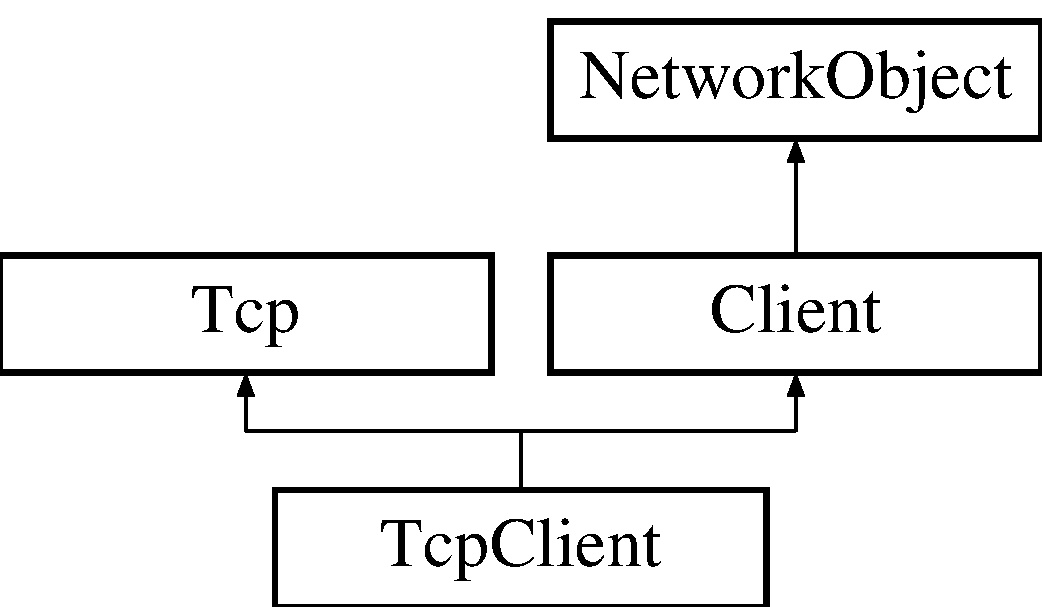
\includegraphics[height=3.000000cm]{classTcpClient}
\end{center}
\end{figure}
\subsection*{Public Member Functions}
\begin{DoxyCompactItemize}
\item 
\hyperlink{classTcpClient_aa1e96bd9ed563f3eaf022cc4e90f91c2}{TcpClient} (const string \&\hyperlink{classTcp_a0e981d15f94a460b91845bce9b930c61}{host}, int \hyperlink{classTcp_a7ed15f78afc9d0675404b4b41cc723ba}{port}, boost::asio::io\_\-service \&\hyperlink{classTcp_ad0c319a0974aa3f07e9c5ae290ea18b4}{io\_\-service})
\item 
\hyperlink{classTcpClient_a1d42085cbb76326fd3698e6924cfbe55}{TcpClient} (const string \&\hyperlink{classTcp_a0e981d15f94a460b91845bce9b930c61}{host}, int \hyperlink{classTcp_a7ed15f78afc9d0675404b4b41cc723ba}{port}, boost::asio::io\_\-service \&\hyperlink{classTcp_ad0c319a0974aa3f07e9c5ae290ea18b4}{io\_\-service}, map$<$ string, string $>$ options)
\item 
virtual \hyperlink{classTcpClient_a125d2277f401cbdebadb9689a5933e18}{$\sim$TcpClient} ()
\item 
virtual void \hyperlink{classTcpClient_a139cffd600eaf851c3560d73a1ba3a54}{send} (const string \&data)
\item 
virtual void \hyperlink{classTcpClient_a1d749cbc2e255d8d3204dfd2d2c58d5f}{send\_\-bytes} (const vector$<$ \hyperlink{Event_8h_ae0aa21f6bcb621fe36c2c962aa0452fe}{byte} $>$ \&bytes)
\item 
virtual void \hyperlink{classTcpClient_a1f0ae8f7c7c12530bc481b77ed984790}{shutdown} ()
\item 
virtual int \hyperlink{classTcpClient_a9caf99246bc1f36dcc69773077ddece8}{get\_\-port} ()
\item 
virtual string \hyperlink{classTcpClient_a4c1ecfdba951d559456c4066a73c8bf6}{get\_\-host} ()
\item 
\hyperlink{classTcpClient_a5275d221f99f3d9702841b461e36108c}{FB\_\-JSAPI\_\-EVENT} (disconnect, 1,(const string \&))
\item 
\hyperlink{classTcpClient_a651d1d61f19169b5755e1716b159eeb8}{FB\_\-JSAPI\_\-EVENT} (connect, 0,())
\end{DoxyCompactItemize}
\subsection*{Protected Member Functions}
\begin{DoxyCompactItemize}
\item 
virtual void \hyperlink{classTcpClient_a03a3ef57b2df46a21e21640362457871}{fire\_\-error\_\-event} (const string \&message)
\item 
virtual void \hyperlink{classTcpClient_a279302da46c29b24b539b4e7ddf20b94}{fire\_\-disconnect\_\-event} (const string \&message)
\item 
virtual void \hyperlink{classTcpClient_a8085a788062b837c12040533a18aa933}{fire\_\-data\_\-event} (const string data, boost::shared\_\-ptr$<$ tcp::socket $>$ \hyperlink{classTcpClient_add183a7de092c7c13ae6ab90766c9881}{connection})
\item 
virtual void \hyperlink{classTcpClient_a1ee082bbca3927811bbe2c0aa75386c4}{close} ()
\end{DoxyCompactItemize}
\subsection*{Private Member Functions}
\begin{DoxyCompactItemize}
\item 
\hyperlink{classTcpClient_a430902765fe325faf409fce8aa3374d2}{TcpClient} (const \hyperlink{classTcpClient}{TcpClient} \&other)
\item 
void \hyperlink{classTcpClient_aeac8e51b95f1ced1141a02ac934bc46d}{init} ()
\item 
void \hyperlink{classTcpClient_a1f9f4dc2af0e396f2c3a46a1e47b68d7}{init\_\-socket} ()
\item 
void \hyperlink{classTcpClient_a4bdf8c1ccee6d9cdb9a2220a95814f0e}{resolve\_\-handler} (const boost::system::error\_\-code \&error\_\-code, tcp::resolver::iterator endpoint\_\-iterator)
\item 
void \hyperlink{classTcpClient_a95419f512dec781b141a4beeea05c9a5}{connect\_\-handler} (const boost::system::error\_\-code \&error\_\-code, tcp::resolver::iterator endpoint\_\-iterator)
\item 
void \hyperlink{classTcpClient_a22407ce44587c805c32009fffe79a95f}{listen} ()
\item 
void \hyperlink{classTcpClient_a8272c8570d9f57b40230ff17b3a42156}{flush} ()
\end{DoxyCompactItemize}
\subsection*{Private Attributes}
\begin{DoxyCompactItemize}
\item 
boost::shared\_\-ptr$<$ tcp::socket $>$ \hyperlink{classTcpClient_add183a7de092c7c13ae6ab90766c9881}{connection}
\item 
boost::shared\_\-ptr$<$ tcp::resolver $>$ \hyperlink{classTcpClient_af3244fcf0139e5a07bd7b85f3e7bb6c9}{resolver}
\item 
bool \hyperlink{classTcpClient_aaceab0b8199fff1898b9c9301748733d}{connected}
\item 
boost::mutex \hyperlink{classTcpClient_a96d0c8fe68ec52f42a1d287356027adb}{connected\_\-mutex}
\item 
queue$<$ string $>$ \hyperlink{classTcpClient_a1ed777da769d6f064d9f908adabf2284}{data\_\-queue}
\item 
boost::mutex \hyperlink{classTcpClient_a158c145cba5559a4e728772b044fbbb8}{data\_\-queue\_\-mutex}
\end{DoxyCompactItemize}


\subsection{Detailed Description}
This class represents a TCP client, which inherits basic TCP handling functionality from {\ttfamily \hyperlink{classTcp}{Tcp}}, and defines additional functionality to resolve and connect to a remote host. 

Definition at line 26 of file TcpClient.h.



\subsection{Constructor \& Destructor Documentation}
\hypertarget{classTcpClient_aa1e96bd9ed563f3eaf022cc4e90f91c2}{
\index{TcpClient@{TcpClient}!TcpClient@{TcpClient}}
\index{TcpClient@{TcpClient}!TcpClient@{TcpClient}}
\subsubsection[{TcpClient}]{\setlength{\rightskip}{0pt plus 5cm}TcpClient::TcpClient (
\begin{DoxyParamCaption}
\item[{const string \&}]{host, }
\item[{int}]{port, }
\item[{boost::asio::io\_\-service \&}]{io\_\-service}
\end{DoxyParamCaption}
)}}
\label{classTcpClient_aa1e96bd9ed563f3eaf022cc4e90f91c2}
Builds a TCP client to connect to a specified remote host and port, and begins asynchronously resolving and connecting to the remote host, given an I/O service to asynchronously perform I/O requests.


\begin{DoxyParams}{Parameters}
{\em host} & The hostname of the remote host to which this client will connect \\
\hline
{\em port} & The port of the remote host to which this client will connect \\
\hline
{\em io\_\-service} & The I/O service to use to perform asynchronous I/O requests \\
\hline
\end{DoxyParams}


Definition at line 10 of file TcpClient.cpp.



References connection, Logger::error(), Tcp::failed, init(), and resolver.


\begin{DoxyCode}
                                                                                 
         :
    Tcp(host, port, io_service), resolver(new tcp::resolver(io_service)), 
      connection(new tcp::socket(io_service))
{
    // Check that the connection and resolver are valid, and fail gracefully if t
      hey are not
    if (!resolver.get() || !connection.get())
    {
        failed = true;
        string message("Failed to initialize TCP client, failed to initialize pro
      perly");
        Logger::error(message, port, host);
        fire_error(message);
        return;
    }

    init();
}
\end{DoxyCode}
\hypertarget{classTcpClient_a1d42085cbb76326fd3698e6924cfbe55}{
\index{TcpClient@{TcpClient}!TcpClient@{TcpClient}}
\index{TcpClient@{TcpClient}!TcpClient@{TcpClient}}
\subsubsection[{TcpClient}]{\setlength{\rightskip}{0pt plus 5cm}TcpClient::TcpClient (
\begin{DoxyParamCaption}
\item[{const string \&}]{host, }
\item[{int}]{port, }
\item[{boost::asio::io\_\-service \&}]{io\_\-service, }
\item[{map$<$ string, string $>$}]{options}
\end{DoxyParamCaption}
)}}
\label{classTcpClient_a1d42085cbb76326fd3698e6924cfbe55}
Builds a TCP client to connect to a specified remote host and port, and begins asynchronously resolving and connecting to the remote host, given an I/O service to asynchronously perform I/O requests.


\begin{DoxyParams}{Parameters}
{\em host} & The hostname of the remote host to which this client will connect \\
\hline
{\em port} & The port of the remote host to which this client will connect \\
\hline
{\em io\_\-service} & The I/O service to use to perform asynchronous I/O requests \\
\hline
{\em options} & A map of options specifying the behavior of the socket \\
\hline
\end{DoxyParams}


Definition at line 26 of file TcpClient.cpp.



References connection, Logger::error(), Tcp::failed, init(), Tcp::parse\_\-args(), and resolver.


\begin{DoxyCode}
                                                                                 
                                      :
    Tcp(host, port, io_service), resolver(new tcp::resolver(io_service)), 
      connection(new tcp::socket(io_service))
{
    // Check that the connection and resolver are valid, and fail gracefully if t
      hey are not
    if (!resolver.get() || !connection.get())
    {
        failed = true;
        string message("Failed to initialize TCP client, failed to initialize pro
      perly");
        Logger::error(message, port, host);
        fire_error(message);
        return;
    }

    parse_args(options);

    init();
}
\end{DoxyCode}
\hypertarget{classTcpClient_a125d2277f401cbdebadb9689a5933e18}{
\index{TcpClient@{TcpClient}!$\sim$TcpClient@{$\sim$TcpClient}}
\index{$\sim$TcpClient@{$\sim$TcpClient}!TcpClient@{TcpClient}}
\subsubsection[{$\sim$TcpClient}]{\setlength{\rightskip}{0pt plus 5cm}TcpClient::$\sim$TcpClient (
\begin{DoxyParamCaption}
{}
\end{DoxyParamCaption}
)\hspace{0.3cm}{\ttfamily  \mbox{[}virtual\mbox{]}}}}
\label{classTcpClient_a125d2277f401cbdebadb9689a5933e18}
Deconstructs a TCP client, immediately calling {\ttfamily close} to shutdown this client's socket and stop listening for responses. 

Definition at line 114 of file TcpClient.cpp.



References close().


\begin{DoxyCode}
{
    close();
}
\end{DoxyCode}
\hypertarget{classTcpClient_a430902765fe325faf409fce8aa3374d2}{
\index{TcpClient@{TcpClient}!TcpClient@{TcpClient}}
\index{TcpClient@{TcpClient}!TcpClient@{TcpClient}}
\subsubsection[{TcpClient}]{\setlength{\rightskip}{0pt plus 5cm}TcpClient::TcpClient (
\begin{DoxyParamCaption}
\item[{const {\bf TcpClient} \&}]{other}
\end{DoxyParamCaption}
)\hspace{0.3cm}{\ttfamily  \mbox{[}private\mbox{]}}}}
\label{classTcpClient_a430902765fe325faf409fce8aa3374d2}
Disallows copying a TCP client 

\subsection{Member Function Documentation}
\hypertarget{classTcpClient_a1ee082bbca3927811bbe2c0aa75386c4}{
\index{TcpClient@{TcpClient}!close@{close}}
\index{close@{close}!TcpClient@{TcpClient}}
\subsubsection[{close}]{\setlength{\rightskip}{0pt plus 5cm}void TcpClient::close (
\begin{DoxyParamCaption}
{}
\end{DoxyParamCaption}
)\hspace{0.3cm}{\ttfamily  \mbox{[}protected, virtual\mbox{]}}}}
\label{classTcpClient_a1ee082bbca3927811bbe2c0aa75386c4}
Immediately cancels any pending operations and closes this client's socket. 

Implements \hyperlink{classTcp_a48b0192669ab99dc953ab3feae5c1b1c}{Tcp}.



Definition at line 119 of file TcpClient.cpp.



References connection, Tcp::host, Tcp::port, resolver, Tcp::waiting\_\-to\_\-shutdown, and Logger::warn().



Referenced by shutdown(), and $\sim$TcpClient().


\begin{DoxyCode}
{
    waiting_to_shutdown = true;
    resolver->cancel();

    // Shutdown the IO service, cancel any transfers on the socket, and close the
       socket
    if (connection->is_open())
    {
        try
        {
            connection->shutdown(connection->shutdown_both);
        }
        catch (...)
        {
            Logger::warn("Socket shutdown improperly, proceeding anyway", port, 
      host);
        }

        connection->close();
    }
    else
    {
        Logger::warn("Failed to cleanly shutdown TCP client connection, continuin
      g anyways", port, host);
    }
}
\end{DoxyCode}
\hypertarget{classTcpClient_a95419f512dec781b141a4beeea05c9a5}{
\index{TcpClient@{TcpClient}!connect\_\-handler@{connect\_\-handler}}
\index{connect\_\-handler@{connect\_\-handler}!TcpClient@{TcpClient}}
\subsubsection[{connect\_\-handler}]{\setlength{\rightskip}{0pt plus 5cm}void TcpClient::connect\_\-handler (
\begin{DoxyParamCaption}
\item[{const boost::system::error\_\-code \&}]{error\_\-code, }
\item[{tcp::resolver::iterator}]{endpoint\_\-iterator}
\end{DoxyParamCaption}
)\hspace{0.3cm}{\ttfamily  \mbox{[}private\mbox{]}}}}
\label{classTcpClient_a95419f512dec781b141a4beeea05c9a5}
I/O handler invoked when this client has attempted to connect to its remote host. If the connection failed, this handler will reattempt the connection by using another resolver if possible, and otherwise fail permanently.


\begin{DoxyParams}{Parameters}
{\em error\_\-code} & The error code encountered when trying to receive data, if any occurred. On success, this value is zero, and nonzero on error. \\
\hline
{\em endpoint\_\-iterator} & Allows the client to iterate through resolvers to retry the connection if it initially fails to connect. \\
\hline
\end{DoxyParams}


Definition at line 278 of file TcpClient.cpp.



References connected, connected\_\-mutex, connection, Tcp::disconnect\_\-errors, Logger::error(), flush(), Tcp::host, Logger::info(), Tcp::port, Tcp::receive\_\-buffer, Tcp::receive\_\-handler(), resolve\_\-handler(), resolver, and Logger::warn().



Referenced by resolve\_\-handler().


\begin{DoxyCode}
{
    // If there was an error to connect, log the error and abort connection
    if (error_code)
    {
        // Check for disconnection errors
        std::set<boost::system::error_code>::iterator find_result = 
      disconnect_errors.find(error_code);
        if (find_result != disconnect_errors.end())
        {
            if (error_code == boost::asio::error::operation_aborted)
            {
                Logger::warn("TCP connect was aborted");
                return;
            }
            else
            {
                string message("TCP connect failed, disconnected: '" + error_code
      .message() + "'");
                Logger::warn(message, port, host);
                fire_disconnect(message);
                return;
            }
        }

        // Check if this was not the last possible connection in the iterator
        tcp::resolver::iterator end;
        if (endpoint_iterator != end && error_code == boost::asio::error::host_no
      t_found)
        {
            // Create a query to resolve this host & port
            tcp::resolver::query query(host, boost::lexical_cast<string>(port));

            // Try the next possible endpoint
            resolver->async_resolve(query, boost::bind(&
      TcpClient::resolve_handler, this, _1, endpoint_iterator++));
        }
        else
        {
            // If we've tried every possible endpoint, fail permanently
            string message("Failed to connect to host, with message: '" + error_c
      ode.message() + "'");
            Logger::error(message, port, host);
            fire_error(message);
            return;
        }
    }

    // Log success, and record that we are now connected
    Logger::info("Connection established to host", port, host);
    fire_connect();

    // Start receiving data on this connection
    connection->async_receive(boost::asio::buffer(receive_buffer),
            boost::bind(&TcpClient::receive_handler, this, _1, _2, connection, 
      host, port));

    // Flush data from the queue if necessary
    flush();

    connected_mutex.lock();

    connected = true;
    connected_mutex.unlock();
}
\end{DoxyCode}
\hypertarget{classTcpClient_a5275d221f99f3d9702841b461e36108c}{
\index{TcpClient@{TcpClient}!FB\_\-JSAPI\_\-EVENT@{FB\_\-JSAPI\_\-EVENT}}
\index{FB\_\-JSAPI\_\-EVENT@{FB\_\-JSAPI\_\-EVENT}!TcpClient@{TcpClient}}
\subsubsection[{FB\_\-JSAPI\_\-EVENT}]{\setlength{\rightskip}{0pt plus 5cm}TcpClient::FB\_\-JSAPI\_\-EVENT (
\begin{DoxyParamCaption}
\item[{disconnect}]{, }
\item[{1}]{, }
\item[{(const string \&)}]{}
\end{DoxyParamCaption}
)}}
\label{classTcpClient_a5275d221f99f3d9702841b461e36108c}
The javascript event fired on a disconnect-\/type network error. This is fired on the following {\ttfamily boost} errors: 
\begin{DoxyItemize}
\item {\ttfamily boost::asio::error::connection\_\-reset} 
\item {\ttfamily boost::asio::error::eof} 
\item {\ttfamily boost::asio::error::connection\_\-aborted} 
\item {\ttfamily boost::asio::error::operation\_\-aborted} 
\end{DoxyItemize}\hypertarget{classTcpClient_a651d1d61f19169b5755e1716b159eeb8}{
\index{TcpClient@{TcpClient}!FB\_\-JSAPI\_\-EVENT@{FB\_\-JSAPI\_\-EVENT}}
\index{FB\_\-JSAPI\_\-EVENT@{FB\_\-JSAPI\_\-EVENT}!TcpClient@{TcpClient}}
\subsubsection[{FB\_\-JSAPI\_\-EVENT}]{\setlength{\rightskip}{0pt plus 5cm}TcpClient::FB\_\-JSAPI\_\-EVENT (
\begin{DoxyParamCaption}
\item[{connect}]{, }
\item[{0}]{, }
\item[{()}]{}
\end{DoxyParamCaption}
)}}
\label{classTcpClient_a651d1d61f19169b5755e1716b159eeb8}
The javascript event fired once a client has connected to its remote endpoint, or once a server has accepted a connection successfully (but has not yet receieved data), in this class, the former. \hypertarget{classTcpClient_a8085a788062b837c12040533a18aa933}{
\index{TcpClient@{TcpClient}!fire\_\-data\_\-event@{fire\_\-data\_\-event}}
\index{fire\_\-data\_\-event@{fire\_\-data\_\-event}!TcpClient@{TcpClient}}
\subsubsection[{fire\_\-data\_\-event}]{\setlength{\rightskip}{0pt plus 5cm}void TcpClient::fire\_\-data\_\-event (
\begin{DoxyParamCaption}
\item[{const string}]{data, }
\item[{boost::shared\_\-ptr$<$ tcp::socket $>$}]{connection}
\end{DoxyParamCaption}
)\hspace{0.3cm}{\ttfamily  \mbox{[}protected, virtual\mbox{]}}}}
\label{classTcpClient_a8085a788062b837c12040533a18aa933}
Helper to fire data event to javascript.


\begin{DoxyParams}{Parameters}
{\em data} & The data received \\
\hline
{\em connection} & The connection on which to reply to the data \\
\hline
\end{DoxyParams}


Implements \hyperlink{classTcp_a7e5cfd764f04ca5e2729924b9d537db2}{Tcp}.



Definition at line 378 of file TcpClient.cpp.


\begin{DoxyCode}
{
    fire_data(boost::make_shared<TcpEvent>(this, connection, data));
}
\end{DoxyCode}
\hypertarget{classTcpClient_a279302da46c29b24b539b4e7ddf20b94}{
\index{TcpClient@{TcpClient}!fire\_\-disconnect\_\-event@{fire\_\-disconnect\_\-event}}
\index{fire\_\-disconnect\_\-event@{fire\_\-disconnect\_\-event}!TcpClient@{TcpClient}}
\subsubsection[{fire\_\-disconnect\_\-event}]{\setlength{\rightskip}{0pt plus 5cm}void TcpClient::fire\_\-disconnect\_\-event (
\begin{DoxyParamCaption}
\item[{const string \&}]{message}
\end{DoxyParamCaption}
)\hspace{0.3cm}{\ttfamily  \mbox{[}protected, virtual\mbox{]}}}}
\label{classTcpClient_a279302da46c29b24b539b4e7ddf20b94}
Helper to fire an disconnect error event to javascript.


\begin{DoxyParams}{Parameters}
{\em message} & The error message \\
\hline
\end{DoxyParams}


Implements \hyperlink{classTcp_a69d92d55403e877f252bbfbfd7c02ec2}{Tcp}.



Definition at line 373 of file TcpClient.cpp.


\begin{DoxyCode}
{
    fire_disconnect(message);
}
\end{DoxyCode}
\hypertarget{classTcpClient_a03a3ef57b2df46a21e21640362457871}{
\index{TcpClient@{TcpClient}!fire\_\-error\_\-event@{fire\_\-error\_\-event}}
\index{fire\_\-error\_\-event@{fire\_\-error\_\-event}!TcpClient@{TcpClient}}
\subsubsection[{fire\_\-error\_\-event}]{\setlength{\rightskip}{0pt plus 5cm}void TcpClient::fire\_\-error\_\-event (
\begin{DoxyParamCaption}
\item[{const string \&}]{message}
\end{DoxyParamCaption}
)\hspace{0.3cm}{\ttfamily  \mbox{[}protected, virtual\mbox{]}}}}
\label{classTcpClient_a03a3ef57b2df46a21e21640362457871}
Helper to fire an error event to javascript.


\begin{DoxyParams}{Parameters}
{\em message} & The error message \\
\hline
\end{DoxyParams}


Implements \hyperlink{classTcp_a9798750750bc775de9a16d0f148bc002}{Tcp}.



Definition at line 368 of file TcpClient.cpp.


\begin{DoxyCode}
{
    fire_error(message);
}
\end{DoxyCode}
\hypertarget{classTcpClient_a8272c8570d9f57b40230ff17b3a42156}{
\index{TcpClient@{TcpClient}!flush@{flush}}
\index{flush@{flush}!TcpClient@{TcpClient}}
\subsubsection[{flush}]{\setlength{\rightskip}{0pt plus 5cm}void TcpClient::flush (
\begin{DoxyParamCaption}
{}
\end{DoxyParamCaption}
)\hspace{0.3cm}{\ttfamily  \mbox{[}private\mbox{]}}}}
\label{classTcpClient_a8272c8570d9f57b40230ff17b3a42156}
Helper function to flush the queue of data if sends are requested before the client is connected 

Definition at line 338 of file TcpClient.cpp.



References connection, TcpEvent::data, data\_\-queue, data\_\-queue\_\-mutex, Tcp::host, Tcp::port, and Tcp::send\_\-handler().



Referenced by connect\_\-handler(), and send().


\begin{DoxyCode}
{
    data_queue_mutex.lock();
    while (!data_queue.empty())
    {
        data_queue_mutex.unlock();

        // Pull the next data chunk to be sent off the queue
        data_queue_mutex.lock();
        string data = data_queue.front();
        data_queue.pop();
        data_queue_mutex.unlock();

        // Asynchronously send the data across the connection
        connection->async_send(boost::asio::buffer(data.data(), data.size()),
                boost::bind(&TcpClient::send_handler, this, _1, _2, data, host, 
      port, connection));
    }
    data_queue_mutex.unlock();
}
\end{DoxyCode}
\hypertarget{classTcpClient_a4c1ecfdba951d559456c4066a73c8bf6}{
\index{TcpClient@{TcpClient}!get\_\-host@{get\_\-host}}
\index{get\_\-host@{get\_\-host}!TcpClient@{TcpClient}}
\subsubsection[{get\_\-host}]{\setlength{\rightskip}{0pt plus 5cm}string TcpClient::get\_\-host (
\begin{DoxyParamCaption}
\item[{void}]{}
\end{DoxyParamCaption}
)\hspace{0.3cm}{\ttfamily  \mbox{[}virtual\mbox{]}}}}
\label{classTcpClient_a4c1ecfdba951d559456c4066a73c8bf6}
Returns the host to which this client connects 

Implements \hyperlink{classClient_a01e5ea1bae012b2a46e8abd6b0bab704}{Client}.



Definition at line 363 of file TcpClient.cpp.



References Tcp::host.


\begin{DoxyCode}
{
    return host;
}
\end{DoxyCode}
\hypertarget{classTcpClient_a9caf99246bc1f36dcc69773077ddece8}{
\index{TcpClient@{TcpClient}!get\_\-port@{get\_\-port}}
\index{get\_\-port@{get\_\-port}!TcpClient@{TcpClient}}
\subsubsection[{get\_\-port}]{\setlength{\rightskip}{0pt plus 5cm}int TcpClient::get\_\-port (
\begin{DoxyParamCaption}
\item[{void}]{}
\end{DoxyParamCaption}
)\hspace{0.3cm}{\ttfamily  \mbox{[}virtual\mbox{]}}}}
\label{classTcpClient_a9caf99246bc1f36dcc69773077ddece8}
Returns the port of the remote host on which this client connects 

Implements \hyperlink{classClient_ac9e4f13eef6b9a776b2bb6cca9d4f78b}{Client}.



Definition at line 358 of file TcpClient.cpp.



References Tcp::port.


\begin{DoxyCode}
{
    return port;
}
\end{DoxyCode}
\hypertarget{classTcpClient_aeac8e51b95f1ced1141a02ac934bc46d}{
\index{TcpClient@{TcpClient}!init@{init}}
\index{init@{init}!TcpClient@{TcpClient}}
\subsubsection[{init}]{\setlength{\rightskip}{0pt plus 5cm}void TcpClient::init (
\begin{DoxyParamCaption}
{}
\end{DoxyParamCaption}
)\hspace{0.3cm}{\ttfamily  \mbox{[}private\mbox{]}}}}
\label{classTcpClient_aeac8e51b95f1ced1141a02ac934bc46d}
Helper function to initialize this client 

Definition at line 44 of file TcpClient.cpp.



References connected, Logger::error(), Tcp::failed, Tcp::host, Logger::info(), Tcp::log\_\-options(), Tcp::port, resolve\_\-handler(), resolver, and Tcp::using\_\-ipv6.



Referenced by TcpClient().


\begin{DoxyCode}
{
    connected = false;

    Logger::info(
            "Initializing TCP client to host '" + boost::lexical_cast<string>(
      host) + "' on port " + boost::lexical_cast<string>(port),
            port, host);
    log_options();
    Logger::info(
            "Trying to resolve DNS information for host " + boost::lexical_cast<s
      tring>(host) + "', port " + boost::lexical_cast<string>(
                    port), port, host);

    // Create a query to resolve this host & port
    if (using_ipv6 && *using_ipv6)
    {
        // Asynchronously resolve the remote host, and once the host is resolved,
       create a connection
        tcp::resolver::query query(tcp::v6(), host, boost::lexical_cast<string>(
      port),
                boost::asio::ip::resolver_query_base::numeric_service);
        if (resolver.get())
            resolver->async_resolve(query, boost::bind(&
      TcpClient::resolve_handler, this, _1, _2));
        else
        {
            failed = true;
            string message("TCP client failed to resolve, invalid resolver");
            Logger::error(message, port, host);
            fire_error(message);
        }
    }
    else
    {
        // Asynchronously resolve the remote host, and once the host is resolved,
       create a connection
        tcp::resolver::query query(tcp::v4(), host, boost::lexical_cast<string>(
      port),
                boost::asio::ip::resolver_query_base::numeric_service);
        if (resolver.get())
            resolver->async_resolve(query, boost::bind(&
      TcpClient::resolve_handler, this, _1, _2));
        else
        {
            failed = true;
            string message("TCP client failed to resolve, invalid resolver");
            Logger::error(message, port, host);
            fire_error(message);
        }
    }
}
\end{DoxyCode}
\hypertarget{classTcpClient_a1f9f4dc2af0e396f2c3a46a1e47b68d7}{
\index{TcpClient@{TcpClient}!init\_\-socket@{init\_\-socket}}
\index{init\_\-socket@{init\_\-socket}!TcpClient@{TcpClient}}
\subsubsection[{init\_\-socket}]{\setlength{\rightskip}{0pt plus 5cm}void TcpClient::init\_\-socket (
\begin{DoxyParamCaption}
{}
\end{DoxyParamCaption}
)\hspace{0.3cm}{\ttfamily  \mbox{[}private\mbox{]}}}}
\label{classTcpClient_a1f9f4dc2af0e396f2c3a46a1e47b68d7}
Initialize the properties of this socket 

Definition at line 89 of file TcpClient.cpp.



References connection, Tcp::do\_\-not\_\-route, Tcp::keep\_\-alive, Tcp::keep\_\-alive\_\-timeout, Tcp::no\_\-delay, and Tcp::set\_\-tcp\_\-keepalive().



Referenced by resolve\_\-handler().


\begin{DoxyCode}
{
    // Set the socket options for this client's TCP socket
    if (do_not_route)
    {
        boost::asio::socket_base::do_not_route option(*do_not_route);
        connection->set_option(option);
    }
    if (keep_alive)
    {
        boost::asio::socket_base::keep_alive option(*keep_alive);
        connection->set_option(option);
    }
    if (no_delay)
    {
        boost::asio::ip::tcp::no_delay option(*no_delay);
        connection->set_option(option);
    }
    if (keep_alive_timeout)
    {
        // Set the TCP keep-alive timeout - ignores return value
        set_tcp_keepalive(connection);
    }
}
\end{DoxyCode}
\hypertarget{classTcpClient_a22407ce44587c805c32009fffe79a95f}{
\index{TcpClient@{TcpClient}!listen@{listen}}
\index{listen@{listen}!TcpClient@{TcpClient}}
\subsubsection[{listen}]{\setlength{\rightskip}{0pt plus 5cm}void TcpClient::listen (
\begin{DoxyParamCaption}
{}
\end{DoxyParamCaption}
)\hspace{0.3cm}{\ttfamily  \mbox{[}private\mbox{]}}}}
\label{classTcpClient_a22407ce44587c805c32009fffe79a95f}
Helper function that will listen for incoming data on the TCP connection for the client, specifically responses to data already sent. \hypertarget{classTcpClient_a4bdf8c1ccee6d9cdb9a2220a95814f0e}{
\index{TcpClient@{TcpClient}!resolve\_\-handler@{resolve\_\-handler}}
\index{resolve\_\-handler@{resolve\_\-handler}!TcpClient@{TcpClient}}
\subsubsection[{resolve\_\-handler}]{\setlength{\rightskip}{0pt plus 5cm}void TcpClient::resolve\_\-handler (
\begin{DoxyParamCaption}
\item[{const boost::system::error\_\-code \&}]{error\_\-code, }
\item[{tcp::resolver::iterator}]{endpoint\_\-iterator}
\end{DoxyParamCaption}
)\hspace{0.3cm}{\ttfamily  \mbox{[}private\mbox{]}}}}
\label{classTcpClient_a4bdf8c1ccee6d9cdb9a2220a95814f0e}
I/O handler invoked when the remote host is resolved. This handler attempts to asynchronously establish a TCP connection with the remote host.


\begin{DoxyParams}{Parameters}
{\em error\_\-code} & The error code encountered when trying to receive data, if any occurred. On success, this value is zero, and nonzero on error. \\
\hline
{\em endpoint\_\-iterator} & Allows the client to iterate through resolvers to retry the connection if it initially fails to connect. \\
\hline
\end{DoxyParams}


Definition at line 215 of file TcpClient.cpp.



References connect\_\-handler(), connection, Tcp::disconnect\_\-errors, Logger::error(), Tcp::failed, Tcp::host, Logger::info(), init\_\-socket(), Tcp::port, Tcp::using\_\-ipv6, and Logger::warn().



Referenced by connect\_\-handler(), and init().


\begin{DoxyCode}
{
    // If we encountered an error
    if (error_code)
    {
        // Check for disconnection errors
        std::set<boost::system::error_code>::iterator find_result = 
      disconnect_errors.find(error_code);
        if (find_result != disconnect_errors.end())
        {
            if (error_code == boost::asio::error::operation_aborted)
            {
                Logger::warn("TCP resolve was aborted");
                return;
            }
            else
            {
                string message("TCP resolve failed, disconnected: '" + error_code
      .message() + "'");
                Logger::warn(message, port, host);
                fire_disconnect(message);
                return;
            }
        }

        // We failed permanently, fail permanently and log it
        string message("Failed to resolve host with error: " + error_code.message
      ());
        Logger::error(message, port, host);
        fire_error(message);
        return;
    }

    if (connection.get())
    {
        // Attempt to connect to the endpoint, using IPv6 if specified
        tcp::endpoint receiver_endpoint = *endpoint_iterator;
        if (using_ipv6 && *using_ipv6)
        {
            connection->open(tcp::v6());
        }
        else
        {
            connection->open(tcp::v4());
        }

        // Initialize the socket if it's open
        if (!connection->is_open())
            init_socket();

        // Log success
        Logger::info("Host has been resolved, attempting to connect to host", 
      port, host);
        fire_resolve();

        // Try to asynchronously establish a connection to the host
        connection->async_connect(receiver_endpoint, boost::bind(&
      TcpClient::connect_handler, this, _1, endpoint_iterator));
    }
    else
    {
        failed = true;
        string message("TCP client failed to resolve, invalid connection");
        Logger::error(message, port, host);
        fire_error(message);
    }
}
\end{DoxyCode}
\hypertarget{classTcpClient_a139cffd600eaf851c3560d73a1ba3a54}{
\index{TcpClient@{TcpClient}!send@{send}}
\index{send@{send}!TcpClient@{TcpClient}}
\subsubsection[{send}]{\setlength{\rightskip}{0pt plus 5cm}void TcpClient::send (
\begin{DoxyParamCaption}
\item[{const string \&}]{data}
\end{DoxyParamCaption}
)\hspace{0.3cm}{\ttfamily  \mbox{[}virtual\mbox{]}}}}
\label{classTcpClient_a139cffd600eaf851c3560d73a1ba3a54}
Asynchronously sends data to the remote host to which this client is connected.


\begin{DoxyParams}{Parameters}
{\em data} & The data to send across the wire \\
\hline
\end{DoxyParams}


Implements \hyperlink{classClient_ae02f1c7ffac49b7543244da28fbb58aa}{Client}.



Definition at line 177 of file TcpClient.cpp.



References Tcp::active\_\-jobs, Tcp::active\_\-jobs\_\-mutex, connected, connected\_\-mutex, connection, data\_\-queue, data\_\-queue\_\-mutex, Logger::error(), Tcp::failed, flush(), Tcp::host, Tcp::port, and Tcp::send\_\-handler().



Referenced by send\_\-bytes().


\begin{DoxyCode}
{
    if (failed)
    {
        // Log & fire an error
        string message("Trying to send data on a TCP client that has permanently 
      failed!");
        Logger::error(message, port, host);
        return;
    }

    // If we're not already connected, then queue this data to be send
    connected_mutex.lock();
    bool connected_now = connected;
    connected_mutex.unlock();

    if (!connected_now)
    {
        active_jobs_mutex.lock();
        active_jobs++;
        active_jobs_mutex.unlock();
        data_queue_mutex.lock();
        data_queue.push(data);
        data_queue_mutex.unlock();
    }
    else
    {
        // Check if the queue needs to be flushed, and if so, flush it
        flush();

        // Send the data, and record that we've started a new send job
        active_jobs_mutex.lock();
        active_jobs++;
        active_jobs_mutex.unlock();
        connection->async_send(boost::asio::buffer(data.data(), data.size()),
                boost::bind(&TcpClient::send_handler, this, _1, _2, data, host, 
      port, connection));
    }
}
\end{DoxyCode}
\hypertarget{classTcpClient_a1d749cbc2e255d8d3204dfd2d2c58d5f}{
\index{TcpClient@{TcpClient}!send\_\-bytes@{send\_\-bytes}}
\index{send\_\-bytes@{send\_\-bytes}!TcpClient@{TcpClient}}
\subsubsection[{send\_\-bytes}]{\setlength{\rightskip}{0pt plus 5cm}void TcpClient::send\_\-bytes (
\begin{DoxyParamCaption}
\item[{const vector$<$ {\bf byte} $>$ \&}]{bytes}
\end{DoxyParamCaption}
)\hspace{0.3cm}{\ttfamily  \mbox{[}virtual\mbox{]}}}}
\label{classTcpClient_a1d749cbc2e255d8d3204dfd2d2c58d5f}
Asynchronously sends bytes to the remote host to which this client is connected.


\begin{DoxyParams}{Parameters}
{\em bytes} & The bytes of data to send across the wire \\
\hline
\end{DoxyParams}


Implements \hyperlink{classClient_a6d77759bc7022e45a3e4326757bd6b8b}{Client}.



Definition at line 165 of file TcpClient.cpp.



References TcpEvent::data, and send().


\begin{DoxyCode}
{
    string data;

    for (int i = 0; i < bytes.size(); i++)
    {
        data.push_back((unsigned char) bytes[i]);
    }

    send(data);
}
\end{DoxyCode}
\hypertarget{classTcpClient_a1f0ae8f7c7c12530bc481b77ed984790}{
\index{TcpClient@{TcpClient}!shutdown@{shutdown}}
\index{shutdown@{shutdown}!TcpClient@{TcpClient}}
\subsubsection[{shutdown}]{\setlength{\rightskip}{0pt plus 5cm}void TcpClient::shutdown (
\begin{DoxyParamCaption}
{}
\end{DoxyParamCaption}
)\hspace{0.3cm}{\ttfamily  \mbox{[}virtual\mbox{]}}}}
\label{classTcpClient_a1f0ae8f7c7c12530bc481b77ed984790}
Gracefully shutdown this TCP client, waiting until all sends have completed before freeing all resources for this TCP client and shutting down any open connections. This function is exposed the javascript API. 

Implements \hyperlink{classNetworkObject_a2f519457fd87c8a92cf265a2b2883e96}{NetworkObject}.



Definition at line 144 of file TcpClient.cpp.



References Tcp::active\_\-jobs, Tcp::active\_\-jobs\_\-mutex, close(), Logger::error(), Tcp::failed, Tcp::host, Tcp::port, and Tcp::waiting\_\-to\_\-shutdown.


\begin{DoxyCode}
{
    if (!failed)
    {
        active_jobs_mutex.lock();
        int current_jobs = active_jobs;
        active_jobs_mutex.unlock();
        waiting_to_shutdown = true;
        if (current_jobs == 0)
        {
            fire_close();
            close();
        }
    }
    else
    {
        // Log & fire an error
        Logger::error("Trying to start the server listening, but the server has p
      ermanently failed!", port, host);
    }
}
\end{DoxyCode}


\subsection{Member Data Documentation}
\hypertarget{classTcpClient_aaceab0b8199fff1898b9c9301748733d}{
\index{TcpClient@{TcpClient}!connected@{connected}}
\index{connected@{connected}!TcpClient@{TcpClient}}
\subsubsection[{connected}]{\setlength{\rightskip}{0pt plus 5cm}bool {\bf TcpClient::connected}\hspace{0.3cm}{\ttfamily  \mbox{[}private\mbox{]}}}}
\label{classTcpClient_aaceab0b8199fff1898b9c9301748733d}
A flag recording whether this client is connected yet or not, used to queue send requests made before this client is connected if necessary. 

Definition at line 197 of file TcpClient.h.



Referenced by connect\_\-handler(), init(), and send().

\hypertarget{classTcpClient_a96d0c8fe68ec52f42a1d287356027adb}{
\index{TcpClient@{TcpClient}!connected\_\-mutex@{connected\_\-mutex}}
\index{connected\_\-mutex@{connected\_\-mutex}!TcpClient@{TcpClient}}
\subsubsection[{connected\_\-mutex}]{\setlength{\rightskip}{0pt plus 5cm}boost::mutex {\bf TcpClient::connected\_\-mutex}\hspace{0.3cm}{\ttfamily  \mbox{[}private\mbox{]}}}}
\label{classTcpClient_a96d0c8fe68ec52f42a1d287356027adb}
A mutex used to access the queue for pending jobs 

Definition at line 202 of file TcpClient.h.



Referenced by connect\_\-handler(), and send().

\hypertarget{classTcpClient_add183a7de092c7c13ae6ab90766c9881}{
\index{TcpClient@{TcpClient}!connection@{connection}}
\index{connection@{connection}!TcpClient@{TcpClient}}
\subsubsection[{connection}]{\setlength{\rightskip}{0pt plus 5cm}boost::shared\_\-ptr$<$tcp::socket$>$ {\bf TcpClient::connection}\hspace{0.3cm}{\ttfamily  \mbox{[}private\mbox{]}}}}
\label{classTcpClient_add183a7de092c7c13ae6ab90766c9881}
A shared reference to the socket used to connect to the remote host 

Definition at line 186 of file TcpClient.h.



Referenced by close(), connect\_\-handler(), flush(), init\_\-socket(), resolve\_\-handler(), send(), and TcpClient().

\hypertarget{classTcpClient_a1ed777da769d6f064d9f908adabf2284}{
\index{TcpClient@{TcpClient}!data\_\-queue@{data\_\-queue}}
\index{data\_\-queue@{data\_\-queue}!TcpClient@{TcpClient}}
\subsubsection[{data\_\-queue}]{\setlength{\rightskip}{0pt plus 5cm}queue$<$string$>$ {\bf TcpClient::data\_\-queue}\hspace{0.3cm}{\ttfamily  \mbox{[}private\mbox{]}}}}
\label{classTcpClient_a1ed777da769d6f064d9f908adabf2284}
A queue of data to be sent, which fills as 'send' or 'send\_\-bytes' commands occur before the client is connected 

Definition at line 207 of file TcpClient.h.



Referenced by flush(), and send().

\hypertarget{classTcpClient_a158c145cba5559a4e728772b044fbbb8}{
\index{TcpClient@{TcpClient}!data\_\-queue\_\-mutex@{data\_\-queue\_\-mutex}}
\index{data\_\-queue\_\-mutex@{data\_\-queue\_\-mutex}!TcpClient@{TcpClient}}
\subsubsection[{data\_\-queue\_\-mutex}]{\setlength{\rightskip}{0pt plus 5cm}boost::mutex {\bf TcpClient::data\_\-queue\_\-mutex}\hspace{0.3cm}{\ttfamily  \mbox{[}private\mbox{]}}}}
\label{classTcpClient_a158c145cba5559a4e728772b044fbbb8}
A mutex used to access the queue for pending jobs 

Definition at line 212 of file TcpClient.h.



Referenced by flush(), and send().

\hypertarget{classTcpClient_af3244fcf0139e5a07bd7b85f3e7bb6c9}{
\index{TcpClient@{TcpClient}!resolver@{resolver}}
\index{resolver@{resolver}!TcpClient@{TcpClient}}
\subsubsection[{resolver}]{\setlength{\rightskip}{0pt plus 5cm}boost::shared\_\-ptr$<$tcp::resolver$>$ {\bf TcpClient::resolver}\hspace{0.3cm}{\ttfamily  \mbox{[}private\mbox{]}}}}
\label{classTcpClient_af3244fcf0139e5a07bd7b85f3e7bb6c9}
Resolver object provided by {\ttfamily boost} to resolve the remote hostname and port 

Definition at line 191 of file TcpClient.h.



Referenced by close(), connect\_\-handler(), init(), and TcpClient().



The documentation for this class was generated from the following files:\begin{DoxyCompactItemize}
\item 
/home/jtedesco/dev/sockit/src/tcp/\hyperlink{TcpClient_8h}{TcpClient.h}\item 
/home/jtedesco/dev/sockit/src/tcp/\hyperlink{TcpClient_8cpp}{TcpClient.cpp}\end{DoxyCompactItemize}

\hypertarget{classTcpEvent}{
\section{TcpEvent Class Reference}
\label{classTcpEvent}\index{TcpEvent@{TcpEvent}}
}


{\ttfamily \#include $<$TcpEvent.h$>$}

Inheritance diagram for TcpEvent:\begin{figure}[H]
\begin{center}
\leavevmode
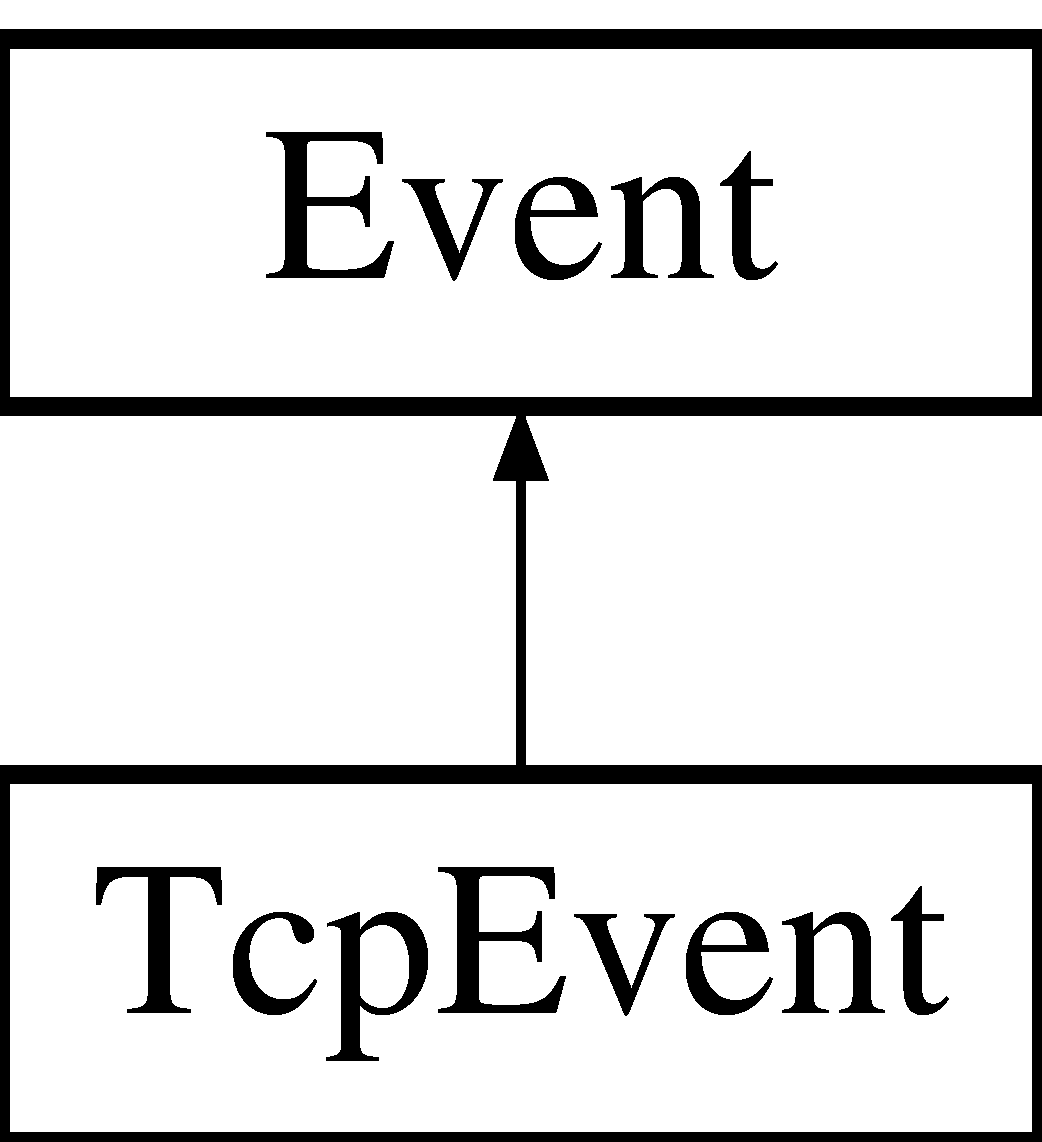
\includegraphics[height=2.000000cm]{classTcpEvent}
\end{center}
\end{figure}
\subsection*{Public Member Functions}
\begin{DoxyCompactItemize}
\item 
\hyperlink{classTcpEvent_a83e2a8e7a05da24e41bfd957f6699959}{TcpEvent} (\hyperlink{classTcp}{Tcp} $\ast$tcp, boost::shared\_\-ptr$<$ tcp::socket $>$ \hyperlink{classTcpEvent_a0cb428ee778cb7c867360b13617011c8}{connection}, string \hyperlink{classTcpEvent_ade7277f4c6339286ea9551183630ee4c}{data})
\item 
virtual \hyperlink{classTcpEvent_a43d6c207a513f1e0e9b917df277a248b}{$\sim$TcpEvent} ()
\item 
virtual void \hyperlink{classTcpEvent_ac9e73ac6ebadc8712d3edfec5e4b1dc9}{send} (const string \&\hyperlink{classTcpEvent_ade7277f4c6339286ea9551183630ee4c}{data})
\item 
virtual void \hyperlink{classTcpEvent_ab6741ad9135b421c220e7601939ea925}{send\_\-bytes} (const vector$<$ \hyperlink{Event_8h_ae0aa21f6bcb621fe36c2c962aa0452fe}{byte} $>$ \&bytes)
\item 
virtual string \hyperlink{classTcpEvent_abc8541d2f0e5b0fbf15191392fbb4a20}{read} () const 
\item 
virtual FB::VariantList \hyperlink{classTcpEvent_adcbbf4231886db58d1df95357b249a26}{read\_\-bytes} () const 
\item 
virtual string \hyperlink{classTcpEvent_a47be6347ecf372f3fbf934ba489d90c1}{get\_\-host} ()
\item 
virtual unsigned short \hyperlink{classTcpEvent_aa14fbf8c465c3487e7eae02ec8815093}{get\_\-port} ()
\end{DoxyCompactItemize}
\subsection*{Private Attributes}
\begin{DoxyCompactItemize}
\item 
string \hyperlink{classTcpEvent_ade7277f4c6339286ea9551183630ee4c}{data}
\item 
bool \hyperlink{classTcpEvent_a80a093f4eab107723fbb0d45414f0a58}{failed}
\item 
\hyperlink{classTcp}{Tcp} $\ast$ \hyperlink{classTcpEvent_ade4fbb5b8a07ec56098fb3301f5ac7a1}{tcp\_\-object}
\item 
string \hyperlink{classTcpEvent_a64ff43fff8e7488f4c4c7bccebbf2d0d}{host}
\item 
int \hyperlink{classTcpEvent_a32b592e6367f3a43a6a66884d94c3d9c}{port}
\item 
boost::shared\_\-ptr$<$ tcp::socket $>$ \hyperlink{classTcpEvent_a0cb428ee778cb7c867360b13617011c8}{connection}
\end{DoxyCompactItemize}


\subsection{Detailed Description}
A TCP implementation of a event to allow javascript to respond to data on a TCP connection.

\begin{DoxySeeAlso}{See also}
\hyperlink{classEvent}{Event} 
\end{DoxySeeAlso}


Definition at line 25 of file TcpEvent.h.



\subsection{Constructor \& Destructor Documentation}
\hypertarget{classTcpEvent_a83e2a8e7a05da24e41bfd957f6699959}{
\index{TcpEvent@{TcpEvent}!TcpEvent@{TcpEvent}}
\index{TcpEvent@{TcpEvent}!TcpEvent@{TcpEvent}}
\subsubsection[{TcpEvent}]{\setlength{\rightskip}{0pt plus 5cm}TcpEvent::TcpEvent (
\begin{DoxyParamCaption}
\item[{{\bf Tcp} $\ast$}]{tcp, }
\item[{boost::shared\_\-ptr$<$ tcp::socket $>$}]{connection, }
\item[{string}]{data}
\end{DoxyParamCaption}
)}}
\label{classTcpEvent_a83e2a8e7a05da24e41bfd957f6699959}
Constructs a new {\ttfamily \hyperlink{classTcpEvent}{TcpEvent}} object containing the TCP connection on which to reply.


\begin{DoxyParams}{Parameters}
{\em tcp} & The TCP server or client associated with this event \\
\hline
{\em connection} & The TCP connection on which to reply \\
\hline
{\em data} & The data received when this event was fired \\
\hline
\end{DoxyParams}


Definition at line 12 of file TcpEvent.cpp.



References Logger::error(), failed, host, and port.


\begin{DoxyCode}
                                                                                 
            :
    tcp_object(tcp_object), connection(connection), failed(false), data(data)
{
    // Check to see if any the parameters are null, and log and fail if this occu
      rs
    if(tcp_object && connection)
    {
        // Initialize only if it's safe
        port = connection->remote_endpoint().port();
        host = connection->remote_endpoint().address().to_string();
    }
    else
    {
        // Fail permanently and log it
        failed = true;

        string message("TCP event was not properly initialized, permanently faile
      d.");
        Logger::error(message, port, host);
        fire_error(message);
    }
}
\end{DoxyCode}
\hypertarget{classTcpEvent_a43d6c207a513f1e0e9b917df277a248b}{
\index{TcpEvent@{TcpEvent}!$\sim$TcpEvent@{$\sim$TcpEvent}}
\index{$\sim$TcpEvent@{$\sim$TcpEvent}!TcpEvent@{TcpEvent}}
\subsubsection[{$\sim$TcpEvent}]{\setlength{\rightskip}{0pt plus 5cm}TcpEvent::$\sim$TcpEvent (
\begin{DoxyParamCaption}
{}
\end{DoxyParamCaption}
)\hspace{0.3cm}{\ttfamily  \mbox{[}virtual\mbox{]}}}}
\label{classTcpEvent_a43d6c207a513f1e0e9b917df277a248b}
Deconstructs the TCP event object, after a single reply. 

Definition at line 33 of file TcpEvent.cpp.


\begin{DoxyCode}
{
    // do not free socket, endpoint or tcp here
}
\end{DoxyCode}


\subsection{Member Function Documentation}
\hypertarget{classTcpEvent_a47be6347ecf372f3fbf934ba489d90c1}{
\index{TcpEvent@{TcpEvent}!get\_\-host@{get\_\-host}}
\index{get\_\-host@{get\_\-host}!TcpEvent@{TcpEvent}}
\subsubsection[{get\_\-host}]{\setlength{\rightskip}{0pt plus 5cm}string TcpEvent::get\_\-host (
\begin{DoxyParamCaption}
\item[{void}]{}
\end{DoxyParamCaption}
)\hspace{0.3cm}{\ttfamily  \mbox{[}virtual\mbox{]}}}}
\label{classTcpEvent_a47be6347ecf372f3fbf934ba489d90c1}
Gets the hostname of the remote endpoint of the TCP connection for this {\ttfamily \hyperlink{classTcpEvent}{TcpEvent}}.

\begin{DoxyReturn}{Returns}
The remote hostname of the TCP connection for this {\ttfamily \hyperlink{classTcpEvent}{TcpEvent}} 
\end{DoxyReturn}


Implements \hyperlink{classEvent_ac3fe62061cb4e4552a91be17031fcc2d}{Event}.



Definition at line 91 of file TcpEvent.cpp.



References host.


\begin{DoxyCode}
{
    return host;
}
\end{DoxyCode}
\hypertarget{classTcpEvent_aa14fbf8c465c3487e7eae02ec8815093}{
\index{TcpEvent@{TcpEvent}!get\_\-port@{get\_\-port}}
\index{get\_\-port@{get\_\-port}!TcpEvent@{TcpEvent}}
\subsubsection[{get\_\-port}]{\setlength{\rightskip}{0pt plus 5cm}unsigned short TcpEvent::get\_\-port (
\begin{DoxyParamCaption}
\item[{void}]{}
\end{DoxyParamCaption}
)\hspace{0.3cm}{\ttfamily  \mbox{[}virtual\mbox{]}}}}
\label{classTcpEvent_aa14fbf8c465c3487e7eae02ec8815093}
Gets the port of the remote endpoint of the TCP connection for this {\ttfamily \hyperlink{classTcpEvent}{TcpEvent}}.

\begin{DoxyReturn}{Returns}
The remote port of the TCP connection for this {\ttfamily \hyperlink{classTcpEvent}{TcpEvent}} 
\end{DoxyReturn}


Implements \hyperlink{classEvent_aa23b8454f931fcbe87ed61f1ec70b8e5}{Event}.



Definition at line 96 of file TcpEvent.cpp.



References port.


\begin{DoxyCode}
{
    return port;
}
\end{DoxyCode}
\hypertarget{classTcpEvent_abc8541d2f0e5b0fbf15191392fbb4a20}{
\index{TcpEvent@{TcpEvent}!read@{read}}
\index{read@{read}!TcpEvent@{TcpEvent}}
\subsubsection[{read}]{\setlength{\rightskip}{0pt plus 5cm}string TcpEvent::read (
\begin{DoxyParamCaption}
{}
\end{DoxyParamCaption}
) const\hspace{0.3cm}{\ttfamily  \mbox{[}virtual\mbox{]}}}}
\label{classTcpEvent_abc8541d2f0e5b0fbf15191392fbb4a20}
Reads the string data that belongs to this event.

\begin{DoxyReturn}{Returns}
The string data received when this event was fired 
\end{DoxyReturn}


Implements \hyperlink{classEvent_a9e334d69556816ca38a8f21845d2a1cb}{Event}.



Definition at line 74 of file TcpEvent.cpp.



References data.


\begin{DoxyCode}
{
    return data;
}
\end{DoxyCode}
\hypertarget{classTcpEvent_adcbbf4231886db58d1df95357b249a26}{
\index{TcpEvent@{TcpEvent}!read\_\-bytes@{read\_\-bytes}}
\index{read\_\-bytes@{read\_\-bytes}!TcpEvent@{TcpEvent}}
\subsubsection[{read\_\-bytes}]{\setlength{\rightskip}{0pt plus 5cm}FB::VariantList TcpEvent::read\_\-bytes (
\begin{DoxyParamCaption}
{}
\end{DoxyParamCaption}
) const\hspace{0.3cm}{\ttfamily  \mbox{[}virtual\mbox{]}}}}
\label{classTcpEvent_adcbbf4231886db58d1df95357b249a26}
Reads the byte data that belongs to this event

\begin{DoxyReturn}{Returns}
The byte data received when this event was fired 
\end{DoxyReturn}


Implements \hyperlink{classEvent_a04fa24d70fb7ec47e50e1a71bcedfe75}{Event}.



Definition at line 79 of file TcpEvent.cpp.



References data.


\begin{DoxyCode}
{
    FB::VariantList fb_bytes;

    for (int i = 0; i < data.size(); i++)
    {
        fb_bytes.push_back((unsigned char) (data.data())[i]);
    }

    return fb_bytes;
}
\end{DoxyCode}
\hypertarget{classTcpEvent_ac9e73ac6ebadc8712d3edfec5e4b1dc9}{
\index{TcpEvent@{TcpEvent}!send@{send}}
\index{send@{send}!TcpEvent@{TcpEvent}}
\subsubsection[{send}]{\setlength{\rightskip}{0pt plus 5cm}void TcpEvent::send (
\begin{DoxyParamCaption}
\item[{const string \&}]{data}
\end{DoxyParamCaption}
)\hspace{0.3cm}{\ttfamily  \mbox{[}virtual\mbox{]}}}}
\label{classTcpEvent_ac9e73ac6ebadc8712d3edfec5e4b1dc9}
Replies on the TCP connection with some data.


\begin{DoxyParams}{Parameters}
{\em data} & The data with which to reply \\
\hline
\end{DoxyParams}


Implements \hyperlink{classEvent_ac4eac8e7d44356632b59381929c8978c}{Event}.



Definition at line 50 of file TcpEvent.cpp.



References Tcp::active\_\-jobs, connection, Logger::error(), Tcp::failed, failed, host, port, Tcp::send\_\-handler(), and tcp\_\-object.



Referenced by send\_\-bytes().


\begin{DoxyCode}
{
    // Don't send if we've permanently failed
    if(failed)
    {
        string message("TCP event failed to send, event already failed permanentl
      y");
        Logger::error(message, port, host);
        fire_error(message);
    }

    if(!tcp_object->failed)
    {
        tcp_object->active_jobs++;
        connection->async_send(boost::asio::buffer(data.data(), data.size()),
                boost::bind(&Tcp::send_handler, tcp_object, _1, _2, data, host, 
      port, connection));
    }
    else
    {
        string message("TCP event failed trying to reply on a permanently failed 
      TCP object");
        Logger::error(message, port, host);
        fire_error(message);
    }
}
\end{DoxyCode}
\hypertarget{classTcpEvent_ab6741ad9135b421c220e7601939ea925}{
\index{TcpEvent@{TcpEvent}!send\_\-bytes@{send\_\-bytes}}
\index{send\_\-bytes@{send\_\-bytes}!TcpEvent@{TcpEvent}}
\subsubsection[{send\_\-bytes}]{\setlength{\rightskip}{0pt plus 5cm}void TcpEvent::send\_\-bytes (
\begin{DoxyParamCaption}
\item[{const vector$<$ {\bf byte} $>$ \&}]{bytes}
\end{DoxyParamCaption}
)\hspace{0.3cm}{\ttfamily  \mbox{[}virtual\mbox{]}}}}
\label{classTcpEvent_ab6741ad9135b421c220e7601939ea925}
Replies on the TCP connection with some data.


\begin{DoxyParams}{Parameters}
{\em bytes} & The bytes of data with which to reply \\
\hline
\end{DoxyParams}


Implements \hyperlink{classEvent_ac2183e14a4f65b18d046a5e082f68e71}{Event}.



Definition at line 38 of file TcpEvent.cpp.



References data, and send().


\begin{DoxyCode}
{
    string data;

    for (int i = 0; i < bytes.size(); i++)
    {
        data.push_back((unsigned char) bytes[i]);
    }

    send(data);
}
\end{DoxyCode}


\subsection{Member Data Documentation}
\hypertarget{classTcpEvent_a0cb428ee778cb7c867360b13617011c8}{
\index{TcpEvent@{TcpEvent}!connection@{connection}}
\index{connection@{connection}!TcpEvent@{TcpEvent}}
\subsubsection[{connection}]{\setlength{\rightskip}{0pt plus 5cm}boost::shared\_\-ptr$<$tcp::socket$>$ {\bf TcpEvent::connection}\hspace{0.3cm}{\ttfamily  \mbox{[}private\mbox{]}}}}
\label{classTcpEvent_a0cb428ee778cb7c867360b13617011c8}
The TCP connection on which to reply 

Definition at line 115 of file TcpEvent.h.



Referenced by send().

\hypertarget{classTcpEvent_ade7277f4c6339286ea9551183630ee4c}{
\index{TcpEvent@{TcpEvent}!data@{data}}
\index{data@{data}!TcpEvent@{TcpEvent}}
\subsubsection[{data}]{\setlength{\rightskip}{0pt plus 5cm}string {\bf TcpEvent::data}\hspace{0.3cm}{\ttfamily  \mbox{[}private\mbox{]}}}}
\label{classTcpEvent_ade7277f4c6339286ea9551183630ee4c}
The data received when this event was fired 

Definition at line 90 of file TcpEvent.h.



Referenced by TcpClient::flush(), read(), read\_\-bytes(), send\_\-bytes(), and TcpClient::send\_\-bytes().

\hypertarget{classTcpEvent_a80a093f4eab107723fbb0d45414f0a58}{
\index{TcpEvent@{TcpEvent}!failed@{failed}}
\index{failed@{failed}!TcpEvent@{TcpEvent}}
\subsubsection[{failed}]{\setlength{\rightskip}{0pt plus 5cm}bool {\bf TcpEvent::failed}\hspace{0.3cm}{\ttfamily  \mbox{[}private\mbox{]}}}}
\label{classTcpEvent_a80a093f4eab107723fbb0d45414f0a58}
A flag to prevent this event from blowing up if was initialized improperly 

Definition at line 95 of file TcpEvent.h.



Referenced by send(), and TcpEvent().

\hypertarget{classTcpEvent_a64ff43fff8e7488f4c4c7bccebbf2d0d}{
\index{TcpEvent@{TcpEvent}!host@{host}}
\index{host@{host}!TcpEvent@{TcpEvent}}
\subsubsection[{host}]{\setlength{\rightskip}{0pt plus 5cm}string {\bf TcpEvent::host}\hspace{0.3cm}{\ttfamily  \mbox{[}private\mbox{]}}}}
\label{classTcpEvent_a64ff43fff8e7488f4c4c7bccebbf2d0d}
The remote hostname of the TCP connection for this {\ttfamily \hyperlink{classTcpEvent}{TcpEvent}} 

Definition at line 105 of file TcpEvent.h.



Referenced by get\_\-host(), send(), and TcpEvent().

\hypertarget{classTcpEvent_a32b592e6367f3a43a6a66884d94c3d9c}{
\index{TcpEvent@{TcpEvent}!port@{port}}
\index{port@{port}!TcpEvent@{TcpEvent}}
\subsubsection[{port}]{\setlength{\rightskip}{0pt plus 5cm}int {\bf TcpEvent::port}\hspace{0.3cm}{\ttfamily  \mbox{[}private\mbox{]}}}}
\label{classTcpEvent_a32b592e6367f3a43a6a66884d94c3d9c}
The remote port of the TCP connection for this {\ttfamily \hyperlink{classTcpEvent}{TcpEvent}}. 

Definition at line 110 of file TcpEvent.h.



Referenced by get\_\-port(), send(), and TcpEvent().

\hypertarget{classTcpEvent_ade4fbb5b8a07ec56098fb3301f5ac7a1}{
\index{TcpEvent@{TcpEvent}!tcp\_\-object@{tcp\_\-object}}
\index{tcp\_\-object@{tcp\_\-object}!TcpEvent@{TcpEvent}}
\subsubsection[{tcp\_\-object}]{\setlength{\rightskip}{0pt plus 5cm}{\bf Tcp}$\ast$ {\bf TcpEvent::tcp\_\-object}\hspace{0.3cm}{\ttfamily  \mbox{[}private\mbox{]}}}}
\label{classTcpEvent_ade4fbb5b8a07ec56098fb3301f5ac7a1}
The TCP server or client associated with this event 

Definition at line 100 of file TcpEvent.h.



Referenced by send().



The documentation for this class was generated from the following files:\begin{DoxyCompactItemize}
\item 
/home/jtedesco/dev/sockit/src/tcp/\hyperlink{TcpEvent_8h}{TcpEvent.h}\item 
/home/jtedesco/dev/sockit/src/tcp/\hyperlink{TcpEvent_8cpp}{TcpEvent.cpp}\end{DoxyCompactItemize}

\hypertarget{classTcpServer}{
\section{TcpServer Class Reference}
\label{classTcpServer}\index{TcpServer@{TcpServer}}
}


{\ttfamily \#include $<$TcpServer.h$>$}

Inheritance diagram for TcpServer:\begin{figure}[H]
\begin{center}
\leavevmode
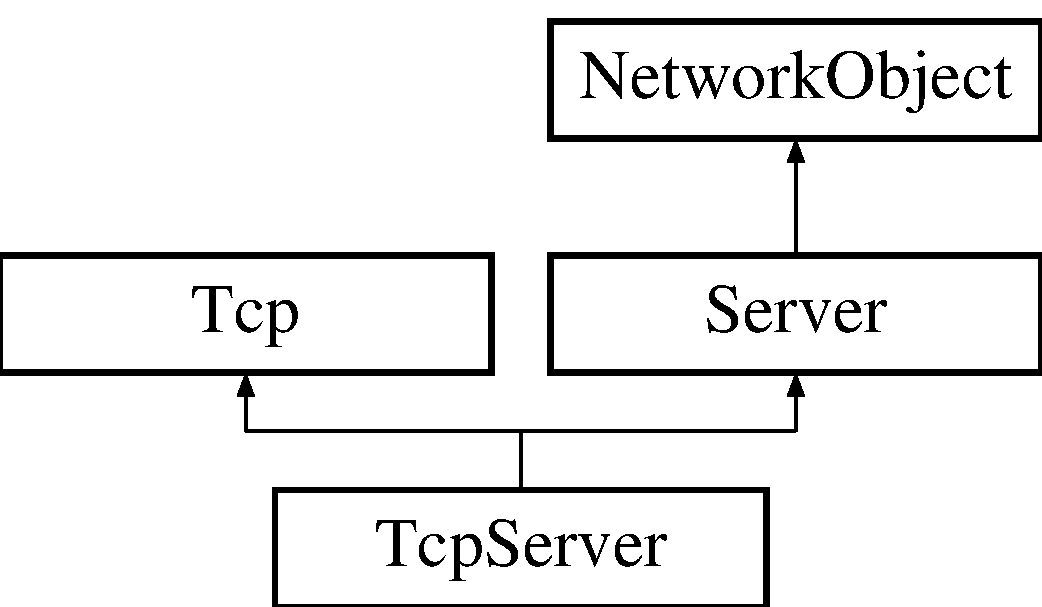
\includegraphics[height=3.000000cm]{classTcpServer}
\end{center}
\end{figure}
\subsection*{Public Member Functions}
\begin{DoxyCompactItemize}
\item 
\hyperlink{classTcpServer_a6c573fc4b33ec7c841afb400a061a08f}{TcpServer} (int \hyperlink{classTcp_a7ed15f78afc9d0675404b4b41cc723ba}{port}, boost::asio::io\_\-service \&\hyperlink{classTcp_ad0c319a0974aa3f07e9c5ae290ea18b4}{io\_\-service})
\item 
\hyperlink{classTcpServer_a7b8c4471aba48774b338b5bc5c4cb310}{TcpServer} (int \hyperlink{classTcp_a7ed15f78afc9d0675404b4b41cc723ba}{port}, boost::asio::io\_\-service \&\hyperlink{classTcp_ad0c319a0974aa3f07e9c5ae290ea18b4}{io\_\-service}, map$<$ string, string $>$ options)
\item 
virtual \hyperlink{classTcpServer_a728a9e31c53cf86887f1f6149b1c46dd}{$\sim$TcpServer} ()
\item 
virtual void \hyperlink{classTcpServer_ad16f797335dd9c54eaec93c35d158569}{start\_\-listening} ()
\item 
virtual void \hyperlink{classTcpServer_a918898ee7b13d776a2f7ea8968168669}{shutdown} ()
\item 
virtual int \hyperlink{classTcpServer_a65be01f9466447530de3112d538267b4}{get\_\-port} ()
\item 
\hyperlink{classTcpServer_afb381d332f0169ac7b1dc3d97de93239}{FB\_\-JSAPI\_\-EVENT} (disconnect, 1,(const string \&))
\item 
\hyperlink{classTcpServer_a0ef55e7e09a51df56c4d1a76e4bda573}{FB\_\-JSAPI\_\-EVENT} (connect, 0,())
\end{DoxyCompactItemize}
\subsection*{Protected Member Functions}
\begin{DoxyCompactItemize}
\item 
void \hyperlink{classTcpServer_a99739644296c7c2647022695d0d0bdbe}{receive\_\-handler} (const boost::system::error\_\-code \&error\_\-code, std::size\_\-t bytesTransferred, boost::shared\_\-ptr$<$ tcp::socket $>$ connection, string \hyperlink{classTcp_a0e981d15f94a460b91845bce9b930c61}{host}, int \hyperlink{classTcp_a7ed15f78afc9d0675404b4b41cc723ba}{port})
\item 
virtual void \hyperlink{classTcpServer_a07ef4a083656e07099f615d34d3627a1}{fire\_\-error\_\-event} (const string \&message)
\item 
virtual void \hyperlink{classTcpServer_aef3b4f4665d3fab448008201915f1fd5}{fire\_\-disconnect\_\-event} (const string \&message)
\item 
virtual void \hyperlink{classTcpServer_a49708224d7eb73b2371b53d672b626e5}{fire\_\-data\_\-event} (const string data, boost::shared\_\-ptr$<$ tcp::socket $>$ connection)
\item 
virtual void \hyperlink{classTcpServer_a6e94bd28e3d3d506609df98afb94c879}{close} ()
\end{DoxyCompactItemize}
\subsection*{Private Member Functions}
\begin{DoxyCompactItemize}
\item 
void \hyperlink{classTcpServer_a64291f0ad4b590f32414ca93fffd13f0}{init} ()
\item 
void \hyperlink{classTcpServer_a6906e0426ba0dc59b4103478a886be46}{init\_\-socket} (boost::shared\_\-ptr$<$ tcp::socket $>$ connection)
\item 
\hyperlink{classTcpServer_abf9de49e9fca80c26eb5143bea332eaa}{TcpServer} (const \hyperlink{classTcpServer}{TcpServer} \&other)
\item 
void \hyperlink{classTcpServer_ac07bb7a42599e9f90f67a11bcba2285e}{accept\_\-handler} (const boost::system::error\_\-code \&error\_\-code, boost::shared\_\-ptr$<$ tcp::socket $>$ connection, string \hyperlink{classTcp_a0e981d15f94a460b91845bce9b930c61}{host}, int \hyperlink{classTcp_a7ed15f78afc9d0675404b4b41cc723ba}{port})
\end{DoxyCompactItemize}
\subsection*{Private Attributes}
\begin{DoxyCompactItemize}
\item 
boost::shared\_\-ptr$<$ tcp::acceptor $>$ \hyperlink{classTcpServer_aa6b754f18b1c444bf6f1af263be18f33}{acceptor}
\item 
set$<$ boost::shared\_\-ptr$<$ tcp::socket $>$ $>$ \hyperlink{classTcpServer_a1beafdc19eb3f4e18fb811057afe5f6d}{connections}
\end{DoxyCompactItemize}


\subsection{Detailed Description}
This class represents a TCP server, which inherits basic TCP handling functionality from {\ttfamily \hyperlink{classTcp}{Tcp}}, and defines additional functionality to bind to a port and accept incoming connections. 

Definition at line 24 of file TcpServer.h.



\subsection{Constructor \& Destructor Documentation}
\hypertarget{classTcpServer_a6c573fc4b33ec7c841afb400a061a08f}{
\index{TcpServer@{TcpServer}!TcpServer@{TcpServer}}
\index{TcpServer@{TcpServer}!TcpServer@{TcpServer}}
\subsubsection[{TcpServer}]{\setlength{\rightskip}{0pt plus 5cm}TcpServer::TcpServer (
\begin{DoxyParamCaption}
\item[{int}]{port, }
\item[{boost::asio::io\_\-service \&}]{io\_\-service}
\end{DoxyParamCaption}
)}}
\label{classTcpServer_a6c573fc4b33ec7c841afb400a061a08f}
Builds a TCP server to listen on the specified port, but does not start the server listening on it. Using this constructor uses IPv4, given an I/O service to use for asynchronous I/O.


\begin{DoxyParams}{Parameters}
{\em port} & The port on which the server should listen \\
\hline
{\em io\_\-service} & The I/O service to use for background I/O requests \\
\hline
\end{DoxyParams}


Definition at line 10 of file TcpServer.cpp.



References init().


\begin{DoxyCode}
                                                               :
    Tcp("SERVER", port, io_service)
{
    init();
}
\end{DoxyCode}
\hypertarget{classTcpServer_a7b8c4471aba48774b338b5bc5c4cb310}{
\index{TcpServer@{TcpServer}!TcpServer@{TcpServer}}
\index{TcpServer@{TcpServer}!TcpServer@{TcpServer}}
\subsubsection[{TcpServer}]{\setlength{\rightskip}{0pt plus 5cm}TcpServer::TcpServer (
\begin{DoxyParamCaption}
\item[{int}]{port, }
\item[{boost::asio::io\_\-service \&}]{io\_\-service, }
\item[{map$<$ string, string $>$}]{options}
\end{DoxyParamCaption}
)}}
\label{classTcpServer_a7b8c4471aba48774b338b5bc5c4cb310}
Builds a TCP server to listen on the specified port, but does not start the server listening on it. Using this constructor creates a server using IPv6, given an I/O service to use for asynchronous I/O.


\begin{DoxyParams}{Parameters}
{\em port} & The port on which the server should listen \\
\hline
{\em io\_\-service} & The I/O service to use for background I/O requests \\
\hline
{\em options} & A map of options specifying the behavior of the socket \\
\hline
\end{DoxyParams}


Definition at line 16 of file TcpServer.cpp.



References init(), and Tcp::parse\_\-args().


\begin{DoxyCode}
                                                                                 
                 :
    Tcp("SERVER", port, io_service)
{
    parse_args(options);
    init();
}
\end{DoxyCode}
\hypertarget{classTcpServer_a728a9e31c53cf86887f1f6149b1c46dd}{
\index{TcpServer@{TcpServer}!$\sim$TcpServer@{$\sim$TcpServer}}
\index{$\sim$TcpServer@{$\sim$TcpServer}!TcpServer@{TcpServer}}
\subsubsection[{$\sim$TcpServer}]{\setlength{\rightskip}{0pt plus 5cm}TcpServer::$\sim$TcpServer (
\begin{DoxyParamCaption}
{}
\end{DoxyParamCaption}
)\hspace{0.3cm}{\ttfamily  \mbox{[}virtual\mbox{]}}}}
\label{classTcpServer_a728a9e31c53cf86887f1f6149b1c46dd}
Deconstructs this TCP server, by immediately ceasing to accept incoming connections, shutdown all necessary resources. 

Definition at line 23 of file TcpServer.cpp.



References close().


\begin{DoxyCode}
{
    close();
}
\end{DoxyCode}
\hypertarget{classTcpServer_abf9de49e9fca80c26eb5143bea332eaa}{
\index{TcpServer@{TcpServer}!TcpServer@{TcpServer}}
\index{TcpServer@{TcpServer}!TcpServer@{TcpServer}}
\subsubsection[{TcpServer}]{\setlength{\rightskip}{0pt plus 5cm}TcpServer::TcpServer (
\begin{DoxyParamCaption}
\item[{const {\bf TcpServer} \&}]{other}
\end{DoxyParamCaption}
)\hspace{0.3cm}{\ttfamily  \mbox{[}private\mbox{]}}}}
\label{classTcpServer_abf9de49e9fca80c26eb5143bea332eaa}
Disallows copying a TCP server 

\subsection{Member Function Documentation}
\hypertarget{classTcpServer_ac07bb7a42599e9f90f67a11bcba2285e}{
\index{TcpServer@{TcpServer}!accept\_\-handler@{accept\_\-handler}}
\index{accept\_\-handler@{accept\_\-handler}!TcpServer@{TcpServer}}
\subsubsection[{accept\_\-handler}]{\setlength{\rightskip}{0pt plus 5cm}void TcpServer::accept\_\-handler (
\begin{DoxyParamCaption}
\item[{const boost::system::error\_\-code \&}]{error\_\-code, }
\item[{boost::shared\_\-ptr$<$ tcp::socket $>$}]{connection, }
\item[{string}]{host, }
\item[{int}]{port}
\end{DoxyParamCaption}
)\hspace{0.3cm}{\ttfamily  \mbox{[}private\mbox{]}}}}
\label{classTcpServer_ac07bb7a42599e9f90f67a11bcba2285e}
Handler invoked when a new connection is made to this server. This handler tries to start receiving data from the new incoming connection if there was no error accepting the connection.


\begin{DoxyParams}{Parameters}
{\em error\_\-code} & The error code encountered when trying to receive data, if any occurred. On success, this value is zero, and nonzero on error. \\
\hline
{\em connection} & The new connection created by this accept, from which this function will attempt to receive data. \\
\hline
{\em host} & The host from which this accept was attempted \\
\hline
{\em port} & The port from which this accept was attempted \\
\hline
\end{DoxyParams}


Definition at line 218 of file TcpServer.cpp.



References Tcp::disconnect\_\-errors, Logger::error(), Logger::info(), init\_\-socket(), Tcp::receive\_\-buffer, receive\_\-handler(), start\_\-listening(), Tcp::waiting\_\-to\_\-shutdown, and Logger::warn().



Referenced by start\_\-listening().


\begin{DoxyCode}
{
    // Log error & return if there is an error
    if (error_code)
    {
        // Check for disconnection errors
        std::set<boost::system::error_code>::iterator find_result = 
      disconnect_errors.find(error_code);
        if (find_result != disconnect_errors.end())
        {
            if (error_code == boost::asio::error::operation_aborted)
            {
                // If we're waiting to shutdown, this is part of the normal proce
      ss
                if(waiting_to_shutdown)
                {
                    Logger::info("TCP server stopped listening for new connection
      s", port, host);
                }
                else
                {
                    Logger::warn("TCP accept was aborted", port, host);
                }
            }
            else
            {
                string message("TCP accept failed, disconnected: '" + error_code.
      message() + "'");
                Logger::warn(message, port, host);
                fire_disconnect(message);
            }
            return;
        }

        string message("Error accepting incoming connection: '" + error_code.mess
      age() + "'");
        Logger::error(message, port, host);
        fire_error(message);
        return;
    }

    // Initialize the socket options before we start using it
    init_socket(connection);

    // Log that we've successfully accepted a new connection, and fire the 'oncon
      nect' event
    string message("TCP server accepted new connection from " + connection->remot
      e_endpoint().address().to_string() + " port "
            + boost::lexical_cast<string>(connection->remote_endpoint().port()));
      
    Logger::info(message, port, host);
    fire_connect();

    if (connection.get())
        connection->async_receive(boost::asio::buffer(receive_buffer),
                boost::bind(&TcpServer::receive_handler, this, _1, _2, connection
      , host, port));

    // Start listening for new connections, if we're not waiting to close
    if (!waiting_to_shutdown)
    {
        start_listening();
    }
}
\end{DoxyCode}
\hypertarget{classTcpServer_a6e94bd28e3d3d506609df98afb94c879}{
\index{TcpServer@{TcpServer}!close@{close}}
\index{close@{close}!TcpServer@{TcpServer}}
\subsubsection[{close}]{\setlength{\rightskip}{0pt plus 5cm}void TcpServer::close (
\begin{DoxyParamCaption}
{}
\end{DoxyParamCaption}
)\hspace{0.3cm}{\ttfamily  \mbox{[}protected, virtual\mbox{]}}}}
\label{classTcpServer_a6e94bd28e3d3d506609df98afb94c879}
Closes down this TCP server immediately, by immediately ceasing to accept incoming connections, shutdown all necessary resources. 

Implements \hyperlink{classTcp_a48b0192669ab99dc953ab3feae5c1b1c}{Tcp}.



Definition at line 28 of file TcpServer.cpp.



References acceptor, connections, Tcp::host, Tcp::port, Tcp::waiting\_\-to\_\-shutdown, and Logger::warn().



Referenced by shutdown(), and $\sim$TcpServer().


\begin{DoxyCode}
{
    // Shutdown the IO service, cancel any transfers on the socket, and close the
       socket
    waiting_to_shutdown = true;

    set<boost::shared_ptr<tcp::socket> >::iterator it;
    for(it = connections.begin(); it != connections.end(); it++)
    {
        try
        {
            if((*it) && (*it).get() && (*it)->is_open())
            {
                (*it)->close();
            }
        }
        catch(boost::system::error_code &e)
        {
            Logger::warn("Error in TcpServer deconstructor: " + e.message(), 
      port, host);
        }
        catch(std::exception &er)
        {
            Logger::warn("Error in TcpServer deconstructor: " + std::string(er.wh
      at()), port, host);
        }
        catch(...)
        {
            Logger::warn("Error occured that could not be caught");
        }
    }

    connections.clear();

    if (acceptor && acceptor->is_open())
    {
        acceptor->close();
    }
    else
    {
        // Don't fire an error, otherwise the plugin will crash
        string message("Could not cleanly shut down acceptor in TCP server, desct
      ructing anyways");
        Logger::warn(message, port, host);
    }
}
\end{DoxyCode}
\hypertarget{classTcpServer_afb381d332f0169ac7b1dc3d97de93239}{
\index{TcpServer@{TcpServer}!FB\_\-JSAPI\_\-EVENT@{FB\_\-JSAPI\_\-EVENT}}
\index{FB\_\-JSAPI\_\-EVENT@{FB\_\-JSAPI\_\-EVENT}!TcpServer@{TcpServer}}
\subsubsection[{FB\_\-JSAPI\_\-EVENT}]{\setlength{\rightskip}{0pt plus 5cm}TcpServer::FB\_\-JSAPI\_\-EVENT (
\begin{DoxyParamCaption}
\item[{disconnect}]{, }
\item[{1}]{, }
\item[{(const string \&)}]{}
\end{DoxyParamCaption}
)}}
\label{classTcpServer_afb381d332f0169ac7b1dc3d97de93239}
The javascript event fired on a disconnect-\/type network error. This is fired on the following {\ttfamily boost} errors: 
\begin{DoxyItemize}
\item {\ttfamily boost::asio::error::connection\_\-reset} 
\item {\ttfamily boost::asio::error::eof} 
\item {\ttfamily boost::asio::error::connection\_\-aborted} 
\item {\ttfamily boost::asio::error::operation\_\-aborted} 
\end{DoxyItemize}\hypertarget{classTcpServer_a0ef55e7e09a51df56c4d1a76e4bda573}{
\index{TcpServer@{TcpServer}!FB\_\-JSAPI\_\-EVENT@{FB\_\-JSAPI\_\-EVENT}}
\index{FB\_\-JSAPI\_\-EVENT@{FB\_\-JSAPI\_\-EVENT}!TcpServer@{TcpServer}}
\subsubsection[{FB\_\-JSAPI\_\-EVENT}]{\setlength{\rightskip}{0pt plus 5cm}TcpServer::FB\_\-JSAPI\_\-EVENT (
\begin{DoxyParamCaption}
\item[{connect}]{, }
\item[{0}]{, }
\item[{()}]{}
\end{DoxyParamCaption}
)}}
\label{classTcpServer_a0ef55e7e09a51df56c4d1a76e4bda573}
The javascript event fired once a client has connected to its remote endpoint, or once a server has accepted a connection successfully (but has not yet receieved data), in this class, the former. \hypertarget{classTcpServer_a49708224d7eb73b2371b53d672b626e5}{
\index{TcpServer@{TcpServer}!fire\_\-data\_\-event@{fire\_\-data\_\-event}}
\index{fire\_\-data\_\-event@{fire\_\-data\_\-event}!TcpServer@{TcpServer}}
\subsubsection[{fire\_\-data\_\-event}]{\setlength{\rightskip}{0pt plus 5cm}void TcpServer::fire\_\-data\_\-event (
\begin{DoxyParamCaption}
\item[{const string}]{data, }
\item[{boost::shared\_\-ptr$<$ tcp::socket $>$}]{connection}
\end{DoxyParamCaption}
)\hspace{0.3cm}{\ttfamily  \mbox{[}protected, virtual\mbox{]}}}}
\label{classTcpServer_a49708224d7eb73b2371b53d672b626e5}
Helper to fire data event to javascript.


\begin{DoxyParams}{Parameters}
{\em data} & The data received \\
\hline
{\em connection} & The connection on which to reply to the data \\
\hline
\end{DoxyParams}


Implements \hyperlink{classTcp_a7e5cfd764f04ca5e2729924b9d537db2}{Tcp}.



Definition at line 299 of file TcpServer.cpp.


\begin{DoxyCode}
{
    fire_data(boost::make_shared<TcpEvent>(this, connection, data));
}
\end{DoxyCode}
\hypertarget{classTcpServer_aef3b4f4665d3fab448008201915f1fd5}{
\index{TcpServer@{TcpServer}!fire\_\-disconnect\_\-event@{fire\_\-disconnect\_\-event}}
\index{fire\_\-disconnect\_\-event@{fire\_\-disconnect\_\-event}!TcpServer@{TcpServer}}
\subsubsection[{fire\_\-disconnect\_\-event}]{\setlength{\rightskip}{0pt plus 5cm}void TcpServer::fire\_\-disconnect\_\-event (
\begin{DoxyParamCaption}
\item[{const string \&}]{message}
\end{DoxyParamCaption}
)\hspace{0.3cm}{\ttfamily  \mbox{[}protected, virtual\mbox{]}}}}
\label{classTcpServer_aef3b4f4665d3fab448008201915f1fd5}
Helper to fire an disconnect error event to javascript.


\begin{DoxyParams}{Parameters}
{\em message} & The error message \\
\hline
\end{DoxyParams}


Implements \hyperlink{classTcp_a69d92d55403e877f252bbfbfd7c02ec2}{Tcp}.



Definition at line 294 of file TcpServer.cpp.


\begin{DoxyCode}
{
    fire_disconnect(message);
}
\end{DoxyCode}
\hypertarget{classTcpServer_a07ef4a083656e07099f615d34d3627a1}{
\index{TcpServer@{TcpServer}!fire\_\-error\_\-event@{fire\_\-error\_\-event}}
\index{fire\_\-error\_\-event@{fire\_\-error\_\-event}!TcpServer@{TcpServer}}
\subsubsection[{fire\_\-error\_\-event}]{\setlength{\rightskip}{0pt plus 5cm}void TcpServer::fire\_\-error\_\-event (
\begin{DoxyParamCaption}
\item[{const string \&}]{message}
\end{DoxyParamCaption}
)\hspace{0.3cm}{\ttfamily  \mbox{[}protected, virtual\mbox{]}}}}
\label{classTcpServer_a07ef4a083656e07099f615d34d3627a1}
Helper to fire an error event to javascript.


\begin{DoxyParams}{Parameters}
{\em message} & The error message \\
\hline
\end{DoxyParams}


Implements \hyperlink{classTcp_a9798750750bc775de9a16d0f148bc002}{Tcp}.



Definition at line 289 of file TcpServer.cpp.


\begin{DoxyCode}
{
    fire_error(message);
}
\end{DoxyCode}
\hypertarget{classTcpServer_a65be01f9466447530de3112d538267b4}{
\index{TcpServer@{TcpServer}!get\_\-port@{get\_\-port}}
\index{get\_\-port@{get\_\-port}!TcpServer@{TcpServer}}
\subsubsection[{get\_\-port}]{\setlength{\rightskip}{0pt plus 5cm}int TcpServer::get\_\-port (
\begin{DoxyParamCaption}
\item[{void}]{}
\end{DoxyParamCaption}
)\hspace{0.3cm}{\ttfamily  \mbox{[}virtual\mbox{]}}}}
\label{classTcpServer_a65be01f9466447530de3112d538267b4}
Returns the port on which this server listens 

Implements \hyperlink{classServer_abd497ca7e7dc29f8ea4c6ce204839a6d}{Server}.



Definition at line 284 of file TcpServer.cpp.



References Tcp::port.


\begin{DoxyCode}
{
    return port;
}
\end{DoxyCode}
\hypertarget{classTcpServer_a64291f0ad4b590f32414ca93fffd13f0}{
\index{TcpServer@{TcpServer}!init@{init}}
\index{init@{init}!TcpServer@{TcpServer}}
\subsubsection[{init}]{\setlength{\rightskip}{0pt plus 5cm}void TcpServer::init (
\begin{DoxyParamCaption}
{}
\end{DoxyParamCaption}
)\hspace{0.3cm}{\ttfamily  \mbox{[}private\mbox{]}}}}
\label{classTcpServer_a64291f0ad4b590f32414ca93fffd13f0}
Helper function to initialize the acceptor. If this was not successfully initialized, {\ttfamily fail} is true. 

Definition at line 71 of file TcpServer.cpp.



References acceptor, Logger::error(), Tcp::failed, Tcp::host, Tcp::io\_\-service, Tcp::port, and Tcp::using\_\-ipv6.



Referenced by TcpServer().


\begin{DoxyCode}
{
    // Bind the acceptor to the correct port & set the options on this acceptor
    try
    {
        if (using_ipv6 && *using_ipv6)
        {
            acceptor = boost::shared_ptr<tcp::acceptor>(new tcp::acceptor(
      io_service, tcp::endpoint(tcp::v6(), port)));
        }
        else
        {
            acceptor = boost::shared_ptr<tcp::acceptor>(new tcp::acceptor(
      io_service, tcp::endpoint(tcp::v4(), port)));
        }
    }
    catch (boost::system::system_error &e)
    {
        // Catch this error, and fail gracefully
        string message(string("Caught error initializing TCP server: '") + e.what
      () + "'");
        Logger::error(message, port, host);

        // Stop this server from ever doing anything again
        failed = true;
    }

    // Check that acceptor was created successfully
    if (!acceptor.get())
    {
        // Fail gracefully and stop this server from ever doing anything again
        string message("Failed to initialized TCP server acceptor");
        Logger::error(message, port, host);
        failed = true;
    }
}
\end{DoxyCode}
\hypertarget{classTcpServer_a6906e0426ba0dc59b4103478a886be46}{
\index{TcpServer@{TcpServer}!init\_\-socket@{init\_\-socket}}
\index{init\_\-socket@{init\_\-socket}!TcpServer@{TcpServer}}
\subsubsection[{init\_\-socket}]{\setlength{\rightskip}{0pt plus 5cm}void TcpServer::init\_\-socket (
\begin{DoxyParamCaption}
\item[{boost::shared\_\-ptr$<$ tcp::socket $>$}]{connection}
\end{DoxyParamCaption}
)\hspace{0.3cm}{\ttfamily  \mbox{[}private\mbox{]}}}}
\label{classTcpServer_a6906e0426ba0dc59b4103478a886be46}
Initialize the properties of this socket 

Definition at line 105 of file TcpServer.cpp.



References Tcp::do\_\-not\_\-route, Tcp::keep\_\-alive, Tcp::keep\_\-alive\_\-timeout, Tcp::no\_\-delay, and Tcp::set\_\-tcp\_\-keepalive().



Referenced by accept\_\-handler().


\begin{DoxyCode}
{
    // Set the socket options for this client's TCP socket
    if (do_not_route)
    {
        boost::asio::socket_base::do_not_route option(*do_not_route);
        connection->set_option(option);
    }

    // Toggle keep alive (enabled/disabled)
    if (keep_alive)
    {
        boost::asio::socket_base::keep_alive option(*keep_alive);
        connection->set_option(option);
    }
    if (no_delay)
    {
        boost::asio::ip::tcp::no_delay option(*no_delay);
        connection->set_option(option);
    }

    if (keep_alive_timeout)
    {
        // Set the TCP keep-alive timeout - ignores return value
        set_tcp_keepalive(connection);
    }
}
\end{DoxyCode}
\hypertarget{classTcpServer_a99739644296c7c2647022695d0d0bdbe}{
\index{TcpServer@{TcpServer}!receive\_\-handler@{receive\_\-handler}}
\index{receive\_\-handler@{receive\_\-handler}!TcpServer@{TcpServer}}
\subsubsection[{receive\_\-handler}]{\setlength{\rightskip}{0pt plus 5cm}void TcpServer::receive\_\-handler (
\begin{DoxyParamCaption}
\item[{const boost::system::error\_\-code \&}]{error\_\-code, }
\item[{std::size\_\-t}]{bytesTransferred, }
\item[{boost::shared\_\-ptr$<$ tcp::socket $>$}]{connection, }
\item[{string}]{host, }
\item[{int}]{port}
\end{DoxyParamCaption}
)\hspace{0.3cm}{\ttfamily  \mbox{[}protected, virtual\mbox{]}}}}
\label{classTcpServer_a99739644296c7c2647022695d0d0bdbe}
Inherited from \hyperlink{classTcp}{Tcp}. Handler invoked when the data has been sent (or sending terminated in error). 

Reimplemented from \hyperlink{classTcp_a96707e496b0fcef660c3f22fb6efc0fd}{Tcp}.



Definition at line 275 of file TcpServer.cpp.



References connections.



Referenced by accept\_\-handler().


\begin{DoxyCode}
{
    Tcp::receive_handler(error_code, bytesTransferred, connection, host, port);

    if(connection && connection.get() && !connection->is_open())
        connections.erase(connection);
}
\end{DoxyCode}
\hypertarget{classTcpServer_a918898ee7b13d776a2f7ea8968168669}{
\index{TcpServer@{TcpServer}!shutdown@{shutdown}}
\index{shutdown@{shutdown}!TcpServer@{TcpServer}}
\subsubsection[{shutdown}]{\setlength{\rightskip}{0pt plus 5cm}void TcpServer::shutdown (
\begin{DoxyParamCaption}
{}
\end{DoxyParamCaption}
)\hspace{0.3cm}{\ttfamily  \mbox{[}virtual\mbox{]}}}}
\label{classTcpServer_a918898ee7b13d776a2f7ea8968168669}
Gracefully shutdown this TCP server, waiting until all sends have completed before freeing all resources for this TCP server and shutting down any open connections. This function is exposed the javascript API. 

Implements \hyperlink{classNetworkObject_a2f519457fd87c8a92cf265a2b2883e96}{NetworkObject}.



Definition at line 199 of file TcpServer.cpp.



References Tcp::active\_\-jobs, close(), Logger::error(), Tcp::failed, Tcp::host, Tcp::port, and Tcp::waiting\_\-to\_\-shutdown.


\begin{DoxyCode}
{
    if(!failed)
    {
        waiting_to_shutdown = true;
        if (active_jobs == 0)
        {
            fire_close();
            close();
        }
    }
    else
    {
        // Log & fire an error
        string message("Trying to shutdown the TCP server, but the server has per
      manently failed!");
        Logger::error(message, port, host);
    }
}
\end{DoxyCode}
\hypertarget{classTcpServer_ad16f797335dd9c54eaec93c35d158569}{
\index{TcpServer@{TcpServer}!start\_\-listening@{start\_\-listening}}
\index{start\_\-listening@{start\_\-listening}!TcpServer@{TcpServer}}
\subsubsection[{start\_\-listening}]{\setlength{\rightskip}{0pt plus 5cm}void TcpServer::start\_\-listening (
\begin{DoxyParamCaption}
{}
\end{DoxyParamCaption}
)\hspace{0.3cm}{\ttfamily  \mbox{[}virtual\mbox{]}}}}
\label{classTcpServer_ad16f797335dd9c54eaec93c35d158569}
Called to start the the server listening for the first time, fires the 'open' event, and is exposed to the javascript. This should only be called once, and starts the server listening for incoming connections. 

Implements \hyperlink{classServer_ab60269481230955b94dc6405162794b0}{Server}.



Definition at line 164 of file TcpServer.cpp.



References accept\_\-handler(), acceptor, connections, Logger::error(), Tcp::failed, Tcp::host, Logger::info(), Tcp::io\_\-service, Tcp::port, and socket\_\-deallocate().



Referenced by accept\_\-handler().


\begin{DoxyCode}
{
    if(failed)
    {
        // Log & fire an error
        string message("Trying to start the server listening, but the server has 
      permanently failed!");
        Logger::error(message, port, host);
    }

    // Log listening
    Logger::info("TCP server about to start listening for incoming connections on
       port "
            + boost::lexical_cast<string>(port), port, host);

    // Prepare to accept a new connection and asynchronously accept new incoming 
      connections
    boost::shared_ptr < tcp::socket > connection(new tcp::socket(io_service), 
      socket_deallocate);
    connections.insert(connection);

    // Try to accept any new connection
    if(acceptor.get())
    {
        acceptor->async_accept(*connection, boost::bind(&
      TcpServer::accept_handler, this, _1, connection, host, port));
    }
    else
    {
        // Fail gracefully and stop this server from ever doing anything again
        string message("TCP server failed to accept, acceptor invalid");
        Logger::error(message, port, host);
        failed = true;
        return;
    }

    // Callback acknowledging that the server has opened
    fire_open();
}
\end{DoxyCode}


\subsection{Member Data Documentation}
\hypertarget{classTcpServer_aa6b754f18b1c444bf6f1af263be18f33}{
\index{TcpServer@{TcpServer}!acceptor@{acceptor}}
\index{acceptor@{acceptor}!TcpServer@{TcpServer}}
\subsubsection[{acceptor}]{\setlength{\rightskip}{0pt plus 5cm}boost::shared\_\-ptr$<$tcp::acceptor$>$ {\bf TcpServer::acceptor}\hspace{0.3cm}{\ttfamily  \mbox{[}private\mbox{]}}}}
\label{classTcpServer_aa6b754f18b1c444bf6f1af263be18f33}
The acceptor for incoming connections for this server 

Definition at line 159 of file TcpServer.h.



Referenced by close(), init(), and start\_\-listening().

\hypertarget{classTcpServer_a1beafdc19eb3f4e18fb811057afe5f6d}{
\index{TcpServer@{TcpServer}!connections@{connections}}
\index{connections@{connections}!TcpServer@{TcpServer}}
\subsubsection[{connections}]{\setlength{\rightskip}{0pt plus 5cm}set$<$boost::shared\_\-ptr$<$tcp::socket$>$ $>$ {\bf TcpServer::connections}\hspace{0.3cm}{\ttfamily  \mbox{[}private\mbox{]}}}}
\label{classTcpServer_a1beafdc19eb3f4e18fb811057afe5f6d}
A set of established connections. 

Definition at line 162 of file TcpServer.h.



Referenced by close(), receive\_\-handler(), and start\_\-listening().



The documentation for this class was generated from the following files:\begin{DoxyCompactItemize}
\item 
/home/jtedesco/dev/sockit/src/tcp/\hyperlink{TcpServer_8h}{TcpServer.h}\item 
/home/jtedesco/dev/sockit/src/tcp/\hyperlink{TcpServer_8cpp}{TcpServer.cpp}\end{DoxyCompactItemize}

\hypertarget{classUdp}{
\section{Udp Class Reference}
\label{classUdp}\index{Udp@{Udp}}
}


{\ttfamily \#include $<$Udp.h$>$}

Inheritance diagram for Udp:\begin{figure}[H]
\begin{center}
\leavevmode
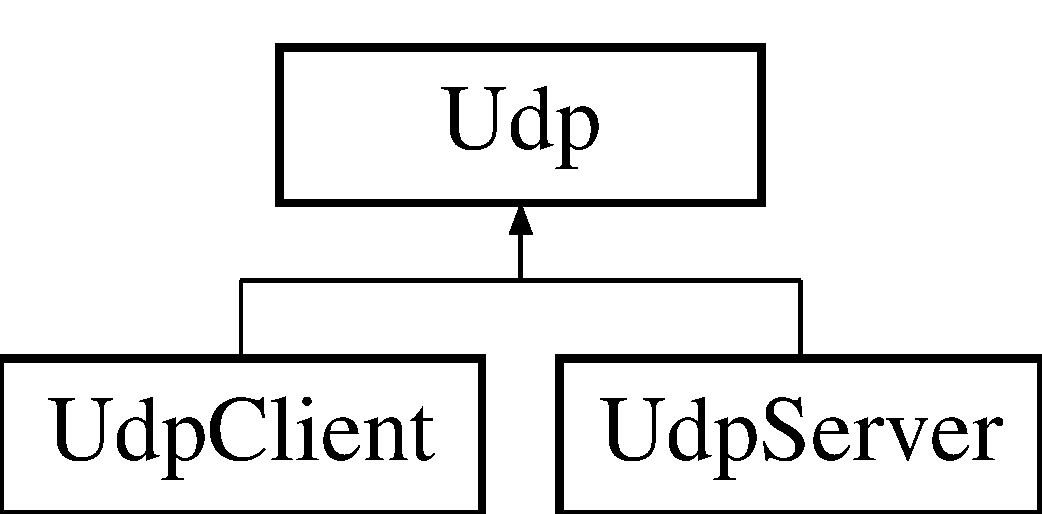
\includegraphics[height=2.000000cm]{classUdp}
\end{center}
\end{figure}
\subsection*{Public Member Functions}
\begin{DoxyCompactItemize}
\item 
\hyperlink{classUdp_a9a7578235269c76bf6d810b7ac1eb268}{Udp} (string \hyperlink{classUdp_a798fd48815d9d97045e8e6a3a290d301}{host}, int \hyperlink{classUdp_af69ea781b31a1fa62e5d3012b6288dc8}{port}, boost::asio::io\_\-service \&\hyperlink{classUdp_a7e143116ab3a0f478c8461ca04af782b}{io\_\-service})
\item 
virtual \hyperlink{classUdp_a74976ab6af022569ab20089c317d0cb6}{$\sim$Udp} ()
\end{DoxyCompactItemize}
\subsection*{Protected Member Functions}
\begin{DoxyCompactItemize}
\item 
string \hyperlink{classUdp_a5fd51bb7cc419e81b873053d7e6b262f}{bool\_\-option\_\-to\_\-string} (optional$<$ bool $>$ \&arg, string iftrue, string iffalse)
\item 
{\footnotesize template$<$class T $>$ }\\string \hyperlink{classUdp_afefa55570fcf5adc18fc131437f31390}{option\_\-to\_\-string} (optional$<$ T $>$ \&arg)
\item 
void \hyperlink{classUdp_ab1af87966ec4c68e8958844f95a75e47}{parse\_\-string\_\-bool\_\-arg} (map$<$ string, string $>$ \&options, string arg, optional$<$ bool $>$ \&arg\_\-value)
\item 
void \hyperlink{classUdp_a19fe0f8b3b2f75cee6ae2841b032c64e}{parse\_\-args} (map$<$ string, string $>$ options)
\item 
void \hyperlink{classUdp_aa3def7bb682cc264bb2e425d93517e17}{log\_\-options} ()
\item 
virtual void \hyperlink{classUdp_a645a7a67007362e349cacc78f9870954}{listen} ()=0
\item 
virtual void \hyperlink{classUdp_a035ec772c3af57eba9d69cf3ba9dcdda}{close} ()=0
\item 
void \hyperlink{classUdp_a8c7b302089f5dd3979b5e1572b190ca8}{send\_\-handler} (const boost::system::error\_\-code \&err, std::size\_\-t bytes\_\-transferred, string msg, string \hyperlink{classUdp_a798fd48815d9d97045e8e6a3a290d301}{host}, int \hyperlink{classUdp_af69ea781b31a1fa62e5d3012b6288dc8}{port})
\item 
void \hyperlink{classUdp_a1edcafcfd4202b3f9cc5a0724f26fe7a}{receive\_\-handler} (const boost::system::error\_\-code \&err, std::size\_\-t bytes\_\-transferred, boost::shared\_\-ptr$<$ udp::socket $>$ socket, boost::shared\_\-ptr$<$ udp::endpoint $>$ endpoint, string \hyperlink{classUdp_a798fd48815d9d97045e8e6a3a290d301}{host}, int \hyperlink{classUdp_af69ea781b31a1fa62e5d3012b6288dc8}{port})
\item 
virtual void \hyperlink{classUdp_a9b79c3603ee9196623aa93b505bda1f6}{fire\_\-error\_\-event} (const string \&message)=0
\item 
virtual void \hyperlink{classUdp_a08e6e588781ce1e7a4d643b97d63dc5c}{fire\_\-data\_\-event} (const string data, boost::shared\_\-ptr$<$ udp::socket $>$ socket, boost::shared\_\-ptr$<$ udp::endpoint $>$ endpoint)=0
\end{DoxyCompactItemize}
\subsection*{Protected Attributes}
\begin{DoxyCompactItemize}
\item 
boost::asio::io\_\-service \& \hyperlink{classUdp_a7e143116ab3a0f478c8461ca04af782b}{io\_\-service}
\item 
boost::array$<$ char, \hyperlink{classUdp_aa72dc03ed420eee2098841f5998e3c53}{BUFFER\_\-SIZE} $>$ \hyperlink{classUdp_a7f21cfeaaccb297124d7582607981afc}{receive\_\-buffer}
\item 
int \hyperlink{classUdp_ac4b9b234de6090250125a1ea05764014}{pending\_\-sends}
\item 
boost::mutex \hyperlink{classUdp_af67ced15878e36d5dbfa433262876922}{pending\_\-sends\_\-mutex}
\item 
bool \hyperlink{classUdp_a01a27e2a1b252f39cefd61eb81a18220}{should\_\-close}
\item 
optional$<$ bool $>$ \hyperlink{classUdp_a3522427333a9a3520e8c8a207cb1a6f2}{using\_\-ipv6}
\item 
optional$<$ bool $>$ \hyperlink{classUdp_aff2511b739bdeee2875c07305b364042}{multicast}
\item 
optional$<$ string $>$ \hyperlink{classUdp_a012f2fbbab10ad7112b6c727e6951207}{multicast\_\-group}
\item 
optional$<$ int $>$ \hyperlink{classUdp_a11f39b2d209d628bdb52ff461e5898d2}{multicast\_\-ttl}
\item 
optional$<$ bool $>$ \hyperlink{classUdp_ace1cbe1cd248a6ae689848f25c26d9d1}{do\_\-not\_\-route}
\item 
optional$<$ bool $>$ \hyperlink{classUdp_a7572159d5d08e4e85e8a1eeba37eb1b9}{reuse\_\-address}
\item 
string \hyperlink{classUdp_a798fd48815d9d97045e8e6a3a290d301}{host}
\item 
int \hyperlink{classUdp_af69ea781b31a1fa62e5d3012b6288dc8}{port}
\item 
boost::shared\_\-ptr$<$ udp::endpoint $>$ \hyperlink{classUdp_ae7fa8c26a933bf54f13f2230760a17e3}{remote\_\-endpoint}
\item 
bool \hyperlink{classUdp_a91a6ea6959febc662830e818b89ed884}{failed}
\end{DoxyCompactItemize}
\subsection*{Static Protected Attributes}
\begin{DoxyCompactItemize}
\item 
static const int \hyperlink{classUdp_aa72dc03ed420eee2098841f5998e3c53}{BUFFER\_\-SIZE} = 2048
\end{DoxyCompactItemize}
\subsection*{Friends}
\begin{DoxyCompactItemize}
\item 
class \hyperlink{classUdp_aa3db591e179836aff8d4a6d952d43101}{UdpEvent}
\end{DoxyCompactItemize}


\subsection{Detailed Description}
Interface to abstract out the client-\/server model for use in the {\ttfamily \hyperlink{classEvent}{Event}}. Contains common handlers used by both UDP servers and clients.

\begin{DoxySeeAlso}{See also}
\hyperlink{classEvent}{Event} 
\end{DoxySeeAlso}


Definition at line 39 of file Udp.h.



\subsection{Constructor \& Destructor Documentation}
\hypertarget{classUdp_a9a7578235269c76bf6d810b7ac1eb268}{
\index{Udp@{Udp}!Udp@{Udp}}
\index{Udp@{Udp}!Udp@{Udp}}
\subsubsection[{Udp}]{\setlength{\rightskip}{0pt plus 5cm}Udp::Udp (
\begin{DoxyParamCaption}
\item[{string}]{host, }
\item[{int}]{port, }
\item[{boost::asio::io\_\-service \&}]{io\_\-service}
\end{DoxyParamCaption}
)}}
\label{classUdp_a9a7578235269c76bf6d810b7ac1eb268}
Builds a generic UDP object, and registers the 'shutdown' method on the API.


\begin{DoxyParams}{Parameters}
{\em host} & The hostname for this UDP object. For clients, this represents the remote host's hostname, and for servers, defaults to 'localhost'. \\
\hline
{\em port} & The port for this UDP object, which for clients, represents the port of the remote host to which to connect, and for servers, represents the port to which to bind and listen for incoming connections. \\
\hline
{\em io\_\-service} & The I/O service used for asynchronous I/O requests \\
\hline
\end{DoxyParams}


Definition at line 10 of file Udp.cpp.



References remote\_\-endpoint.


\begin{DoxyCode}
                                                                :
    host(host), port(port), pending_sends(0), should_close(false), io_service(
      io_service), failed(false)
{
    remote_endpoint = boost::shared_ptr<udp::endpoint>(new udp::endpoint());
}
\end{DoxyCode}
\hypertarget{classUdp_a74976ab6af022569ab20089c317d0cb6}{
\index{Udp@{Udp}!$\sim$Udp@{$\sim$Udp}}
\index{$\sim$Udp@{$\sim$Udp}!Udp@{Udp}}
\subsubsection[{$\sim$Udp}]{\setlength{\rightskip}{0pt plus 5cm}virtual Udp::$\sim$Udp (
\begin{DoxyParamCaption}
{}
\end{DoxyParamCaption}
)\hspace{0.3cm}{\ttfamily  \mbox{[}inline, virtual\mbox{]}}}}
\label{classUdp_a74976ab6af022569ab20089c317d0cb6}
Immediately calls the {\ttfamily close} function, freeing all resources for this UDP object and shutting down any open connections. 

Definition at line 59 of file Udp.h.


\begin{DoxyCode}
{}
\end{DoxyCode}


\subsection{Member Function Documentation}
\hypertarget{classUdp_a5fd51bb7cc419e81b873053d7e6b262f}{
\index{Udp@{Udp}!bool\_\-option\_\-to\_\-string@{bool\_\-option\_\-to\_\-string}}
\index{bool\_\-option\_\-to\_\-string@{bool\_\-option\_\-to\_\-string}!Udp@{Udp}}
\subsubsection[{bool\_\-option\_\-to\_\-string}]{\setlength{\rightskip}{0pt plus 5cm}string Udp::bool\_\-option\_\-to\_\-string (
\begin{DoxyParamCaption}
\item[{optional$<$ bool $>$ \&}]{arg, }
\item[{string}]{iftrue, }
\item[{string}]{iffalse}
\end{DoxyParamCaption}
)\hspace{0.3cm}{\ttfamily  \mbox{[}inline, protected\mbox{]}}}}
\label{classUdp_a5fd51bb7cc419e81b873053d7e6b262f}
Helper for logging options passed in.


\begin{DoxyParams}{Parameters}
{\em arg} & optional bool option \\
\hline
{\em iftrue} & if the arg has been set to true, return this \\
\hline
{\em iffalse} & if the arg hasn't been set, or is set to false, return this \\
\hline
\end{DoxyParams}


Definition at line 143 of file Udp.cpp.



Referenced by log\_\-options().


\begin{DoxyCode}
{
    if (arg && *arg)
        return iftrue;
    return iffalse;
}
\end{DoxyCode}
\hypertarget{classUdp_a035ec772c3af57eba9d69cf3ba9dcdda}{
\index{Udp@{Udp}!close@{close}}
\index{close@{close}!Udp@{Udp}}
\subsubsection[{close}]{\setlength{\rightskip}{0pt plus 5cm}virtual void Udp::close (
\begin{DoxyParamCaption}
{}
\end{DoxyParamCaption}
)\hspace{0.3cm}{\ttfamily  \mbox{[}protected, pure virtual\mbox{]}}}}
\label{classUdp_a035ec772c3af57eba9d69cf3ba9dcdda}
Immediately frees all resources for this UDP object and shutting down any open connections. This function should never be invoked by the base class, and logs an error if this ever occurs. 

Implemented in \hyperlink{classUdpClient_a48cc5f9ce547f5b0505fb8395ac93d32}{UdpClient}, and \hyperlink{classUdpServer_a020144da72e1f29be85ed99225372b21}{UdpServer}.



Referenced by send\_\-handler().

\hypertarget{classUdp_a08e6e588781ce1e7a4d643b97d63dc5c}{
\index{Udp@{Udp}!fire\_\-data\_\-event@{fire\_\-data\_\-event}}
\index{fire\_\-data\_\-event@{fire\_\-data\_\-event}!Udp@{Udp}}
\subsubsection[{fire\_\-data\_\-event}]{\setlength{\rightskip}{0pt plus 5cm}virtual void Udp::fire\_\-data\_\-event (
\begin{DoxyParamCaption}
\item[{const string}]{data, }
\item[{boost::shared\_\-ptr$<$ udp::socket $>$}]{socket, }
\item[{boost::shared\_\-ptr$<$ udp::endpoint $>$}]{endpoint}
\end{DoxyParamCaption}
)\hspace{0.3cm}{\ttfamily  \mbox{[}protected, pure virtual\mbox{]}}}}
\label{classUdp_a08e6e588781ce1e7a4d643b97d63dc5c}
Helper to fire data event to javascript.


\begin{DoxyParams}{Parameters}
{\em data} & The data received \\
\hline
{\em socket} & The socket on which to reply to this data \\
\hline
{\em endpoint} & The connected endpoint to the remote host \\
\hline
\end{DoxyParams}


Implemented in \hyperlink{classUdpClient_acce4181d7ce20a812fffed395486a1bd}{UdpClient}, and \hyperlink{classUdpServer_ab3bcedec1031181a7dd3affddf3d8447}{UdpServer}.



Referenced by receive\_\-handler().

\hypertarget{classUdp_a9b79c3603ee9196623aa93b505bda1f6}{
\index{Udp@{Udp}!fire\_\-error\_\-event@{fire\_\-error\_\-event}}
\index{fire\_\-error\_\-event@{fire\_\-error\_\-event}!Udp@{Udp}}
\subsubsection[{fire\_\-error\_\-event}]{\setlength{\rightskip}{0pt plus 5cm}virtual void Udp::fire\_\-error\_\-event (
\begin{DoxyParamCaption}
\item[{const string \&}]{message}
\end{DoxyParamCaption}
)\hspace{0.3cm}{\ttfamily  \mbox{[}protected, pure virtual\mbox{]}}}}
\label{classUdp_a9b79c3603ee9196623aa93b505bda1f6}
Helper to fire an error event to javascript.


\begin{DoxyParams}{Parameters}
{\em message} & The error message \\
\hline
\end{DoxyParams}


Implemented in \hyperlink{classUdpClient_ae62b9e08cc550a47bbedca2e4556ebcc}{UdpClient}, and \hyperlink{classUdpServer_aa9a023a74c61ba03af476f12958385df}{UdpServer}.



Referenced by receive\_\-handler(), and send\_\-handler().

\hypertarget{classUdp_a645a7a67007362e349cacc78f9870954}{
\index{Udp@{Udp}!listen@{listen}}
\index{listen@{listen}!Udp@{Udp}}
\subsubsection[{listen}]{\setlength{\rightskip}{0pt plus 5cm}virtual void Udp::listen (
\begin{DoxyParamCaption}
{}
\end{DoxyParamCaption}
)\hspace{0.3cm}{\ttfamily  \mbox{[}protected, pure virtual\mbox{]}}}}
\label{classUdp_a645a7a67007362e349cacc78f9870954}
Helper function to listen for incoming data. 

Implemented in \hyperlink{classUdpClient_ae62759a7050f171fe12413ec658bb38b}{UdpClient}, and \hyperlink{classUdpServer_ad1c4a040a4c510ecd85b9b9c7e61e995}{UdpServer}.



Referenced by receive\_\-handler().

\hypertarget{classUdp_aa3def7bb682cc264bb2e425d93517e17}{
\index{Udp@{Udp}!log\_\-options@{log\_\-options}}
\index{log\_\-options@{log\_\-options}!Udp@{Udp}}
\subsubsection[{log\_\-options}]{\setlength{\rightskip}{0pt plus 5cm}void Udp::log\_\-options (
\begin{DoxyParamCaption}
{}
\end{DoxyParamCaption}
)\hspace{0.3cm}{\ttfamily  \mbox{[}protected\mbox{]}}}}
\label{classUdp_aa3def7bb682cc264bb2e425d93517e17}
Write to the log the options used to create this connection. 

Definition at line 158 of file Udp.cpp.



References bool\_\-option\_\-to\_\-string(), do\_\-not\_\-route, host, Logger::info(), multicast, multicast\_\-group, multicast\_\-ttl, port, reuse\_\-address, and using\_\-ipv6.



Referenced by UdpClient::init\_\-socket(), and UdpServer::initialize().


\begin{DoxyCode}
{
    string options("These arguments were passed in: ");

    options.append(bool_option_to_string(using_ipv6, "ipv6, ", "ipv4, "));
    options.append(bool_option_to_string(multicast, "multicast enabled, ", "multi
      cast disabled, "));
    options.append(bool_option_to_string(do_not_route, "no routing, ", "use routi
      ng, "));
    options.append(bool_option_to_string(reuse_address, "reuse address, ", "don't
       reuse address, "));

    options.append("multicast group: ");
    options.append(option_to_string<string> (multicast_group));

    options.append(", multicast ttl: ");
    options.append(option_to_string<int> (multicast_ttl));

    Logger::info(options, port, host);
}
\end{DoxyCode}
\hypertarget{classUdp_afefa55570fcf5adc18fc131437f31390}{
\index{Udp@{Udp}!option\_\-to\_\-string@{option\_\-to\_\-string}}
\index{option\_\-to\_\-string@{option\_\-to\_\-string}!Udp@{Udp}}
\subsubsection[{option\_\-to\_\-string}]{\setlength{\rightskip}{0pt plus 5cm}template$<$class T $>$ string Udp::option\_\-to\_\-string (
\begin{DoxyParamCaption}
\item[{optional$<$ T $>$ \&}]{arg}
\end{DoxyParamCaption}
)\hspace{0.3cm}{\ttfamily  \mbox{[}inline, protected\mbox{]}}}}
\label{classUdp_afefa55570fcf5adc18fc131437f31390}
Helper for logging options passed in.


\begin{DoxyParams}{Parameters}
{\em arg} & the optional argument \\
\hline
\end{DoxyParams}


Definition at line 151 of file Udp.cpp.


\begin{DoxyCode}
{
    if (arg)
        return boost::lexical_cast<string>(*arg);
    return string("unset");
}
\end{DoxyCode}
\hypertarget{classUdp_a19fe0f8b3b2f75cee6ae2841b032c64e}{
\index{Udp@{Udp}!parse\_\-args@{parse\_\-args}}
\index{parse\_\-args@{parse\_\-args}!Udp@{Udp}}
\subsubsection[{parse\_\-args}]{\setlength{\rightskip}{0pt plus 5cm}void Udp::parse\_\-args (
\begin{DoxyParamCaption}
\item[{map$<$ string, string $>$}]{options}
\end{DoxyParamCaption}
)\hspace{0.3cm}{\ttfamily  \mbox{[}protected\mbox{]}}}}
\label{classUdp_a19fe0f8b3b2f75cee6ae2841b032c64e}
Parses any options (like whether or use IPv6 or IPv4) from the options. Supported options currently include:

ipv6 if true, use ipv6. otherwise use ipv4. multicast enable udp multicasting multicast group the multicast group to join multicast ttl number of multicast hops to make; do not route prevent routing, use local interfaces reuse address allow the socket to bind to an address already in use keep alive allow the socket to send keep-\/alives.


\begin{DoxyParams}{Parameters}
{\em options} & A map of options to values. \\
\hline
\end{DoxyParams}


Definition at line 107 of file Udp.cpp.



References do\_\-not\_\-route, multicast, multicast\_\-group, multicast\_\-ttl, parse\_\-string\_\-bool\_\-arg(), reuse\_\-address, and using\_\-ipv6.



Referenced by UdpClient::UdpClient(), and UdpServer::UdpServer().


\begin{DoxyCode}
{
    map<string, string>::iterator it;
    map<string, string> transformed_options;

    string t("true");
    string f("false");

    // transform the entire map to lower case
    for (it = options.begin(); it != options.end(); it++)
    {
        string k = it->first;
        string v = it->second;

        std::transform(k.begin(), k.end(), k.begin(), ::tolower);
        std::transform(v.begin(), v.end(), v.begin(), ::tolower);

        k.erase(std::remove_if(k.begin(), k.end(), ::isspace), k.end());
        v.erase(std::remove_if(v.begin(), v.end(), ::isspace), v.end());

        transformed_options.insert(std::pair<string, string>(k, v));
    }

    /* Lets just pretend you didn't see any of this */
    parse_string_bool_arg(transformed_options, "ipv6", using_ipv6);
    parse_string_bool_arg(transformed_options, "multicast", multicast);
    parse_string_bool_arg(transformed_options, "donotroute", do_not_route);
    parse_string_bool_arg(transformed_options, "reuseaddress", reuse_address);

    if ((it = transformed_options.find("multicastgroup")) != transformed_options.
      end())
        multicast_group.reset(it->second);

    if ((it = transformed_options.find("multicastttl")) != transformed_options.en
      d())
        multicast_ttl.reset(boost::lexical_cast<int>(it->second));
}
\end{DoxyCode}
\hypertarget{classUdp_ab1af87966ec4c68e8958844f95a75e47}{
\index{Udp@{Udp}!parse\_\-string\_\-bool\_\-arg@{parse\_\-string\_\-bool\_\-arg}}
\index{parse\_\-string\_\-bool\_\-arg@{parse\_\-string\_\-bool\_\-arg}!Udp@{Udp}}
\subsubsection[{parse\_\-string\_\-bool\_\-arg}]{\setlength{\rightskip}{0pt plus 5cm}void Udp::parse\_\-string\_\-bool\_\-arg (
\begin{DoxyParamCaption}
\item[{map$<$ string, string $>$ \&}]{options, }
\item[{string}]{arg, }
\item[{optional$<$ bool $>$ \&}]{arg\_\-value}
\end{DoxyParamCaption}
)\hspace{0.3cm}{\ttfamily  \mbox{[}inline, protected\mbox{]}}}}
\label{classUdp_ab1af87966ec4c68e8958844f95a75e47}
Helper for parsing arguments


\begin{DoxyParams}{Parameters}
{\em options} & A map of strings to string representing the options passed in and their values \\
\hline
{\em arg} & The specific option to check for \\
\hline
{\em arg\_\-value} & This will hold the value of the argument, if found. \\
\hline
\end{DoxyParams}


Definition at line 94 of file Udp.cpp.



Referenced by parse\_\-args().


\begin{DoxyCode}
{
    map<string, string>::iterator it;

    if ((it = options.find(arg)) != options.end())
    {
        if (it->second == std::string("true"))
            arg_value.reset(true);
        if (it->second == std::string("false"))
            arg_value.reset(false);
    }
}
\end{DoxyCode}
\hypertarget{classUdp_a1edcafcfd4202b3f9cc5a0724f26fe7a}{
\index{Udp@{Udp}!receive\_\-handler@{receive\_\-handler}}
\index{receive\_\-handler@{receive\_\-handler}!Udp@{Udp}}
\subsubsection[{receive\_\-handler}]{\setlength{\rightskip}{0pt plus 5cm}void Udp::receive\_\-handler (
\begin{DoxyParamCaption}
\item[{const boost::system::error\_\-code \&}]{err, }
\item[{std::size\_\-t}]{bytes\_\-transferred, }
\item[{boost::shared\_\-ptr$<$ udp::socket $>$}]{socket, }
\item[{boost::shared\_\-ptr$<$ udp::endpoint $>$}]{endpoint, }
\item[{string}]{host, }
\item[{int}]{port}
\end{DoxyParamCaption}
)\hspace{0.3cm}{\ttfamily  \mbox{[}protected\mbox{]}}}}
\label{classUdp_a1edcafcfd4202b3f9cc5a0724f26fe7a}
Handler invoked when some data has been received.


\begin{DoxyParams}{Parameters}
{\em err} & The error code encountered when trying to receive data, if any occurred. On success, this value is zero, and nonzero on error. \\
\hline
{\em bytes\_\-transferred} & The number of bytes successfully received over the connection. \\
\hline
{\em socket} & The connection on which attempted to receive data. \\
\hline
{\em endpoint} & The connected endpoint to the remote host \\
\hline
{\em host} & The hostname for this UDP object \\
\hline
{\em port} & The port for this UDP object \\
\hline
\end{DoxyParams}


Definition at line 59 of file Udp.cpp.



References Logger::error(), fire\_\-data\_\-event(), fire\_\-error\_\-event(), Logger::info(), listen(), receive\_\-buffer, and should\_\-close.



Referenced by UdpServer::listen(), and UdpClient::listen().


\begin{DoxyCode}
{
    // Check for errors
    if (error_code)
    {
        if (error_code == boost::asio::error::operation_aborted)
        {
            Logger::info("UDP receive failed, aborted", port, host);
        }
        else
        {
            string message(
                    "UDP receive failed, error message: '" + error_code.message()
       + "', code: '" + boost::lexical_cast<string>(
                            error_code.value()) + "'");
            Logger::error(message, port, host);
            fire_error_event(message);
        }

        return;
    }

    // Get the data && fire a data event
    string data(receive_buffer.c_array(), bytes_transferred);
    fire_data_event(data, socket, endpoint);

    // Pull out the data we received, and fire a data received event
    Logger::info("UDP receive succeeded, received " + boost::lexical_cast<string>
      (bytes_transferred) + " bytes, data is: " + data, port,
            host);

    // Listen for more messages if we're not trying to close down this UDP object
      
    if (!should_close)
        listen();
}
\end{DoxyCode}
\hypertarget{classUdp_a8c7b302089f5dd3979b5e1572b190ca8}{
\index{Udp@{Udp}!send\_\-handler@{send\_\-handler}}
\index{send\_\-handler@{send\_\-handler}!Udp@{Udp}}
\subsubsection[{send\_\-handler}]{\setlength{\rightskip}{0pt plus 5cm}void Udp::send\_\-handler (
\begin{DoxyParamCaption}
\item[{const boost::system::error\_\-code \&}]{err, }
\item[{std::size\_\-t}]{bytes\_\-transferred, }
\item[{string}]{msg, }
\item[{string}]{host, }
\item[{int}]{port}
\end{DoxyParamCaption}
)\hspace{0.3cm}{\ttfamily  \mbox{[}protected\mbox{]}}}}
\label{classUdp_a8c7b302089f5dd3979b5e1572b190ca8}
Handler invoked when the data has been sent (or sending terminated in error).


\begin{DoxyParams}{Parameters}
{\em err} & The error code encountered when trying to send data, if any occurred. On success, this value is zero, and nonzero on error. \\
\hline
{\em bytes\_\-transferred} & The number of bytes successfully sent over the connection. \\
\hline
{\em msg} & The data to be sent. \\
\hline
{\em host} & The hostname for this UDP object \\
\hline
{\em port} & The port for this UDP object \\
\hline
\end{DoxyParams}


Definition at line 16 of file Udp.cpp.



References close(), Logger::error(), fire\_\-error\_\-event(), Logger::info(), pending\_\-sends, pending\_\-sends\_\-mutex, and should\_\-close.



Referenced by UdpEvent::send(), and UdpClient::send().


\begin{DoxyCode}
{
    if (error_code)
    {
        if (error_code == boost::asio::error::operation_aborted)
        {
            Logger::info("UDP send failed, aborted", port, host);
        }
        else
        {
            string message(
                    "UDP send failed, error message: '" + error_code.message() + 
      "', error code '" + boost::lexical_cast<string>(
                            error_code.value()) + "' was encountered");
            Logger::error(message, port, host);
            fire_error_event(message);
        }
        return;
    }

    // Did not successfully send all the data, don't try and resend the rest (thi
      s is UDP)
    if (bytes_transferred != data.size())
    {
        string message(
                string("UDP send failed, data was not successfully sent, only ") 
      + boost::lexical_cast<string>(bytes_transferred) + " of "
                        + boost::lexical_cast<string>(message.size()) + " total b
      ytes were sent");
        Logger::error(message, port, host);
        fire_error_event(message);

        return;
    }

    string message("UDP send succeeded, sent " + boost::lexical_cast<string>(byte
      s_transferred) + " bytes, message is: " + data);
    Logger::info(message, port, host);

    pending_sends_mutex.lock();
    pending_sends--; // just handled sending
    int pending_sends_now = pending_sends;
    pending_sends_mutex.unlock();

    if (pending_sends_now == 0 && should_close)
        close();
}
\end{DoxyCode}


\subsection{Friends And Related Function Documentation}
\hypertarget{classUdp_aa3db591e179836aff8d4a6d952d43101}{
\index{Udp@{Udp}!UdpEvent@{UdpEvent}}
\index{UdpEvent@{UdpEvent}!Udp@{Udp}}
\subsubsection[{UdpEvent}]{\setlength{\rightskip}{0pt plus 5cm}friend class {\bf UdpEvent}\hspace{0.3cm}{\ttfamily  \mbox{[}friend\mbox{]}}}}
\label{classUdp_aa3db591e179836aff8d4a6d952d43101}


Reimplemented in \hyperlink{classUdpServer_aa3db591e179836aff8d4a6d952d43101}{UdpServer}.



Definition at line 61 of file Udp.h.



\subsection{Member Data Documentation}
\hypertarget{classUdp_aa72dc03ed420eee2098841f5998e3c53}{
\index{Udp@{Udp}!BUFFER\_\-SIZE@{BUFFER\_\-SIZE}}
\index{BUFFER\_\-SIZE@{BUFFER\_\-SIZE}!Udp@{Udp}}
\subsubsection[{BUFFER\_\-SIZE}]{\setlength{\rightskip}{0pt plus 5cm}const int {\bf Udp::BUFFER\_\-SIZE} = 2048\hspace{0.3cm}{\ttfamily  \mbox{[}static, protected\mbox{]}}}}
\label{classUdp_aa72dc03ed420eee2098841f5998e3c53}
A constant representing the size of the buffer in which to receive data. This is adjust to support the largest packet possible according to the UDP protocol. 

Definition at line 171 of file Udp.h.



Referenced by UdpClient::init\_\-socket(), and UdpServer::initialize().

\hypertarget{classUdp_ace1cbe1cd248a6ae689848f25c26d9d1}{
\index{Udp@{Udp}!do\_\-not\_\-route@{do\_\-not\_\-route}}
\index{do\_\-not\_\-route@{do\_\-not\_\-route}!Udp@{Udp}}
\subsubsection[{do\_\-not\_\-route}]{\setlength{\rightskip}{0pt plus 5cm}optional$<$bool$>$ {\bf Udp::do\_\-not\_\-route}\hspace{0.3cm}{\ttfamily  \mbox{[}protected\mbox{]}}}}
\label{classUdp_ace1cbe1cd248a6ae689848f25c26d9d1}
Flag to prevent routing, use local interfaces only 

Definition at line 198 of file Udp.h.



Referenced by UdpClient::init\_\-socket(), UdpServer::initialize(), log\_\-options(), and parse\_\-args().

\hypertarget{classUdp_a91a6ea6959febc662830e818b89ed884}{
\index{Udp@{Udp}!failed@{failed}}
\index{failed@{failed}!Udp@{Udp}}
\subsubsection[{failed}]{\setlength{\rightskip}{0pt plus 5cm}bool {\bf Udp::failed}\hspace{0.3cm}{\ttfamily  \mbox{[}protected\mbox{]}}}}
\label{classUdp_a91a6ea6959febc662830e818b89ed884}
A flag to say if this UDP object has permanently failed and cannot continue for some reason or another 

Definition at line 213 of file Udp.h.



Referenced by UdpEvent::send(), UdpClient::send(), UdpServer::shutdown(), UdpClient::shutdown(), UdpServer::start\_\-listening(), and UdpClient::UdpClient().

\hypertarget{classUdp_a798fd48815d9d97045e8e6a3a290d301}{
\index{Udp@{Udp}!host@{host}}
\index{host@{host}!Udp@{Udp}}
\subsubsection[{host}]{\setlength{\rightskip}{0pt plus 5cm}string {\bf Udp::host}\hspace{0.3cm}{\ttfamily  \mbox{[}protected\mbox{]}}}}
\label{classUdp_a798fd48815d9d97045e8e6a3a290d301}
The hostname for this UDP object ('SERVER' for servers, or the hostname of the remote host for clients) 

Definition at line 204 of file Udp.h.



Referenced by UdpClient::get\_\-host(), UdpClient::init\_\-socket(), UdpServer::initialize(), UdpServer::listen(), UdpClient::listen(), log\_\-options(), UdpClient::resolve\_\-handler(), UdpClient::send(), UdpServer::shutdown(), and UdpServer::start\_\-listening().

\hypertarget{classUdp_a7e143116ab3a0f478c8461ca04af782b}{
\index{Udp@{Udp}!io\_\-service@{io\_\-service}}
\index{io\_\-service@{io\_\-service}!Udp@{Udp}}
\subsubsection[{io\_\-service}]{\setlength{\rightskip}{0pt plus 5cm}boost::asio::io\_\-service\& {\bf Udp::io\_\-service}\hspace{0.3cm}{\ttfamily  \mbox{[}protected\mbox{]}}}}
\label{classUdp_a7e143116ab3a0f478c8461ca04af782b}
The I/O service for perform nonblocking actions 

Definition at line 167 of file Udp.h.

\hypertarget{classUdp_aff2511b739bdeee2875c07305b364042}{
\index{Udp@{Udp}!multicast@{multicast}}
\index{multicast@{multicast}!Udp@{Udp}}
\subsubsection[{multicast}]{\setlength{\rightskip}{0pt plus 5cm}optional$<$bool$>$ {\bf Udp::multicast}\hspace{0.3cm}{\ttfamily  \mbox{[}protected\mbox{]}}}}
\label{classUdp_aff2511b739bdeee2875c07305b364042}
Flag representing whether or not multicast is enabled for this UDP object. 

Definition at line 189 of file Udp.h.



Referenced by UdpClient::init\_\-socket(), UdpServer::initialize(), log\_\-options(), parse\_\-args(), and UdpServer::start\_\-listening().

\hypertarget{classUdp_a012f2fbbab10ad7112b6c727e6951207}{
\index{Udp@{Udp}!multicast\_\-group@{multicast\_\-group}}
\index{multicast\_\-group@{multicast\_\-group}!Udp@{Udp}}
\subsubsection[{multicast\_\-group}]{\setlength{\rightskip}{0pt plus 5cm}optional$<$string$>$ {\bf Udp::multicast\_\-group}\hspace{0.3cm}{\ttfamily  \mbox{[}protected\mbox{]}}}}
\label{classUdp_a012f2fbbab10ad7112b6c727e6951207}
If multicast is enabled, use this for the group to join 

Definition at line 192 of file Udp.h.



Referenced by log\_\-options(), parse\_\-args(), and UdpServer::start\_\-listening().

\hypertarget{classUdp_a11f39b2d209d628bdb52ff461e5898d2}{
\index{Udp@{Udp}!multicast\_\-ttl@{multicast\_\-ttl}}
\index{multicast\_\-ttl@{multicast\_\-ttl}!Udp@{Udp}}
\subsubsection[{multicast\_\-ttl}]{\setlength{\rightskip}{0pt plus 5cm}optional$<$int$>$ {\bf Udp::multicast\_\-ttl}\hspace{0.3cm}{\ttfamily  \mbox{[}protected\mbox{]}}}}
\label{classUdp_a11f39b2d209d628bdb52ff461e5898d2}
If multicast is enabled, this is the TTL or hops 

Definition at line 195 of file Udp.h.



Referenced by UdpClient::init\_\-socket(), UdpServer::initialize(), log\_\-options(), and parse\_\-args().

\hypertarget{classUdp_ac4b9b234de6090250125a1ea05764014}{
\index{Udp@{Udp}!pending\_\-sends@{pending\_\-sends}}
\index{pending\_\-sends@{pending\_\-sends}!Udp@{Udp}}
\subsubsection[{pending\_\-sends}]{\setlength{\rightskip}{0pt plus 5cm}int {\bf Udp::pending\_\-sends}\hspace{0.3cm}{\ttfamily  \mbox{[}protected\mbox{]}}}}
\label{classUdp_ac4b9b234de6090250125a1ea05764014}
The number of asynchronous I/O requests that are pending completion 

Definition at line 177 of file Udp.h.



Referenced by UdpEvent::send(), UdpClient::send(), send\_\-handler(), UdpServer::shutdown(), and UdpClient::shutdown().

\hypertarget{classUdp_af67ced15878e36d5dbfa433262876922}{
\index{Udp@{Udp}!pending\_\-sends\_\-mutex@{pending\_\-sends\_\-mutex}}
\index{pending\_\-sends\_\-mutex@{pending\_\-sends\_\-mutex}!Udp@{Udp}}
\subsubsection[{pending\_\-sends\_\-mutex}]{\setlength{\rightskip}{0pt plus 5cm}boost::mutex {\bf Udp::pending\_\-sends\_\-mutex}\hspace{0.3cm}{\ttfamily  \mbox{[}protected\mbox{]}}}}
\label{classUdp_af67ced15878e36d5dbfa433262876922}
Mutex for accessing the number of pending sends 

Definition at line 180 of file Udp.h.



Referenced by UdpClient::send(), send\_\-handler(), and UdpClient::shutdown().

\hypertarget{classUdp_af69ea781b31a1fa62e5d3012b6288dc8}{
\index{Udp@{Udp}!port@{port}}
\index{port@{port}!Udp@{Udp}}
\subsubsection[{port}]{\setlength{\rightskip}{0pt plus 5cm}int {\bf Udp::port}\hspace{0.3cm}{\ttfamily  \mbox{[}protected\mbox{]}}}}
\label{classUdp_af69ea781b31a1fa62e5d3012b6288dc8}
The port (the port bound to by servers, port on which to connect to the remote host for clients) 

Definition at line 207 of file Udp.h.



Referenced by UdpServer::get\_\-port(), UdpClient::get\_\-port(), UdpClient::init\_\-socket(), UdpServer::initialize(), UdpServer::listen(), UdpClient::listen(), log\_\-options(), UdpClient::resolve\_\-handler(), UdpClient::send(), UdpServer::shutdown(), and UdpServer::start\_\-listening().

\hypertarget{classUdp_a7f21cfeaaccb297124d7582607981afc}{
\index{Udp@{Udp}!receive\_\-buffer@{receive\_\-buffer}}
\index{receive\_\-buffer@{receive\_\-buffer}!Udp@{Udp}}
\subsubsection[{receive\_\-buffer}]{\setlength{\rightskip}{0pt plus 5cm}boost::array$<$char, {\bf BUFFER\_\-SIZE}$>$ {\bf Udp::receive\_\-buffer}\hspace{0.3cm}{\ttfamily  \mbox{[}protected\mbox{]}}}}
\label{classUdp_a7f21cfeaaccb297124d7582607981afc}
A buffer for receiving data from the remote host. 

Definition at line 174 of file Udp.h.



Referenced by UdpServer::listen(), UdpClient::listen(), and receive\_\-handler().

\hypertarget{classUdp_ae7fa8c26a933bf54f13f2230760a17e3}{
\index{Udp@{Udp}!remote\_\-endpoint@{remote\_\-endpoint}}
\index{remote\_\-endpoint@{remote\_\-endpoint}!Udp@{Udp}}
\subsubsection[{remote\_\-endpoint}]{\setlength{\rightskip}{0pt plus 5cm}boost::shared\_\-ptr$<$udp::endpoint$>$ {\bf Udp::remote\_\-endpoint}\hspace{0.3cm}{\ttfamily  \mbox{[}protected\mbox{]}}}}
\label{classUdp_ae7fa8c26a933bf54f13f2230760a17e3}
A connected endpoint to the remote host. 

Definition at line 210 of file Udp.h.



Referenced by UdpServer::listen(), UdpClient::listen(), UdpClient::resolve\_\-handler(), UdpClient::send(), and Udp().

\hypertarget{classUdp_a7572159d5d08e4e85e8a1eeba37eb1b9}{
\index{Udp@{Udp}!reuse\_\-address@{reuse\_\-address}}
\index{reuse\_\-address@{reuse\_\-address}!Udp@{Udp}}
\subsubsection[{reuse\_\-address}]{\setlength{\rightskip}{0pt plus 5cm}optional$<$bool$>$ {\bf Udp::reuse\_\-address}\hspace{0.3cm}{\ttfamily  \mbox{[}protected\mbox{]}}}}
\label{classUdp_a7572159d5d08e4e85e8a1eeba37eb1b9}
Flag to allow the socket to be bound to an address that is already in use. 

Definition at line 201 of file Udp.h.



Referenced by UdpClient::init\_\-socket(), UdpServer::initialize(), log\_\-options(), and parse\_\-args().

\hypertarget{classUdp_a01a27e2a1b252f39cefd61eb81a18220}{
\index{Udp@{Udp}!should\_\-close@{should\_\-close}}
\index{should\_\-close@{should\_\-close}!Udp@{Udp}}
\subsubsection[{should\_\-close}]{\setlength{\rightskip}{0pt plus 5cm}bool {\bf Udp::should\_\-close}\hspace{0.3cm}{\ttfamily  \mbox{[}protected\mbox{]}}}}
\label{classUdp_a01a27e2a1b252f39cefd61eb81a18220}
A flag indicating whether or not this object has been requested to shutdown. 

Definition at line 183 of file Udp.h.



Referenced by UdpClient::close(), UdpClient::fire\_\-data\_\-event(), UdpClient::fire\_\-error\_\-event(), receive\_\-handler(), UdpClient::send(), send\_\-handler(), UdpServer::shutdown(), and UdpClient::shutdown().

\hypertarget{classUdp_a3522427333a9a3520e8c8a207cb1a6f2}{
\index{Udp@{Udp}!using\_\-ipv6@{using\_\-ipv6}}
\index{using\_\-ipv6@{using\_\-ipv6}!Udp@{Udp}}
\subsubsection[{using\_\-ipv6}]{\setlength{\rightskip}{0pt plus 5cm}optional$<$bool$>$ {\bf Udp::using\_\-ipv6}\hspace{0.3cm}{\ttfamily  \mbox{[}protected\mbox{]}}}}
\label{classUdp_a3522427333a9a3520e8c8a207cb1a6f2}
Flag for using IPv6, if true, this UDP object uses IPv6, otherwise, it is using IPv4. 

Definition at line 186 of file Udp.h.



Referenced by UdpClient::init\_\-socket(), UdpServer::initialize(), log\_\-options(), parse\_\-args(), UdpClient::send(), and UdpServer::start\_\-listening().



The documentation for this class was generated from the following files:\begin{DoxyCompactItemize}
\item 
/home/jtedesco/dev/sockit/src/udp/\hyperlink{Udp_8h}{Udp.h}\item 
/home/jtedesco/dev/sockit/src/udp/\hyperlink{Udp_8cpp}{Udp.cpp}\end{DoxyCompactItemize}

\hypertarget{classUdpClient}{
\section{UdpClient Class Reference}
\label{classUdpClient}\index{UdpClient@{UdpClient}}
}


{\ttfamily \#include $<$UdpClient.h$>$}

Inheritance diagram for UdpClient:\begin{figure}[H]
\begin{center}
\leavevmode
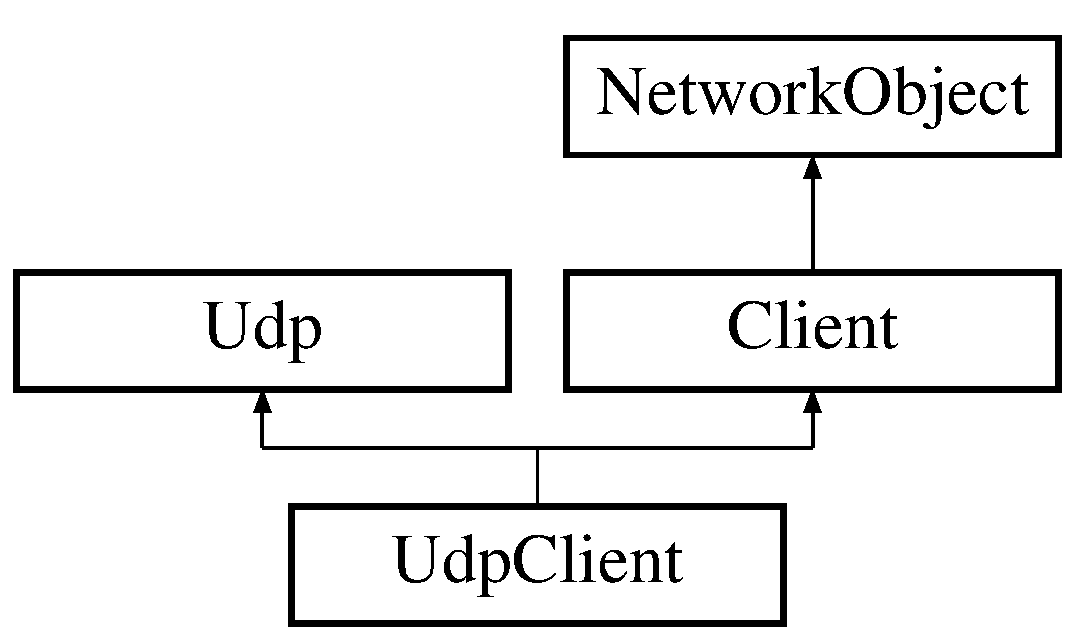
\includegraphics[height=3.000000cm]{classUdpClient}
\end{center}
\end{figure}
\subsection*{Public Member Functions}
\begin{DoxyCompactItemize}
\item 
\hyperlink{classUdpClient_a3939a516b0c78c572bb6318be26039c8}{UdpClient} (const string \&\hyperlink{classUdp_a798fd48815d9d97045e8e6a3a290d301}{host}, int \hyperlink{classUdp_af69ea781b31a1fa62e5d3012b6288dc8}{port}, boost::asio::io\_\-service \&\hyperlink{classUdp_a7e143116ab3a0f478c8461ca04af782b}{io\_\-service})
\item 
\hyperlink{classUdpClient_a3a44547ebe0cbc3b85e0163b32767338}{UdpClient} (const string \&\hyperlink{classUdp_a798fd48815d9d97045e8e6a3a290d301}{host}, int \hyperlink{classUdp_af69ea781b31a1fa62e5d3012b6288dc8}{port}, boost::asio::io\_\-service \&\hyperlink{classUdp_a7e143116ab3a0f478c8461ca04af782b}{io\_\-service}, map$<$ string, string $>$ options)
\item 
virtual \hyperlink{classUdpClient_a9e69046802da8ea9e0bf3da874c49e47}{$\sim$UdpClient} ()
\item 
virtual void \hyperlink{classUdpClient_a86e50f32bbb7aaf657ea5cc91cbc99d2}{send} (const string \&data)
\item 
virtual void \hyperlink{classUdpClient_ad55f42a3c5cb3698b49975c8a065079e}{send\_\-bytes} (const vector$<$ \hyperlink{Event_8h_ae0aa21f6bcb621fe36c2c962aa0452fe}{byte} $>$ \&bytes)
\item 
virtual void \hyperlink{classUdpClient_a64b6b51f6a2316f7235381409f9cc327}{shutdown} ()
\item 
virtual int \hyperlink{classUdpClient_aaa19f0f767306e0e974782dd700c5c49}{get\_\-port} ()
\item 
virtual string \hyperlink{classUdpClient_ac18bd8d30497c82dfe1a63a464d01e00}{get\_\-host} ()
\end{DoxyCompactItemize}
\subsection*{Protected Member Functions}
\begin{DoxyCompactItemize}
\item 
void \hyperlink{classUdpClient_a4c1f1672598ea18294f2486e071e0985}{init\_\-socket} ()
\item 
virtual void \hyperlink{classUdpClient_ae62b9e08cc550a47bbedca2e4556ebcc}{fire\_\-error\_\-event} (const string \&message)
\item 
virtual void \hyperlink{classUdpClient_acce4181d7ce20a812fffed395486a1bd}{fire\_\-data\_\-event} (const string data, boost::shared\_\-ptr$<$ udp::socket $>$ \hyperlink{classUdpClient_a5e929af056033e7b1fd3f72ad2bd1849}{socket}, boost::shared\_\-ptr$<$ udp::endpoint $>$ endpoint)
\item 
virtual void \hyperlink{classUdpClient_a48cc5f9ce547f5b0505fb8395ac93d32}{close} ()
\end{DoxyCompactItemize}
\subsection*{Private Member Functions}
\begin{DoxyCompactItemize}
\item 
\hyperlink{classUdpClient_a2694066d9e432d68eca656f00152278d}{UdpClient} (const \hyperlink{classUdpClient}{UdpClient} \&other)
\item 
virtual void \hyperlink{classUdpClient_ae62759a7050f171fe12413ec658bb38b}{listen} ()
\item 
void \hyperlink{classUdpClient_a16e67afc411590eb1602fc02e3395599}{resolve\_\-handler} (const boost::system::error\_\-code \&err, udp::resolver::iterator endpoint\_\-iterator)
\item 
void \hyperlink{classUdpClient_a755db78b027af8161b0b79563c857f2f}{flush} ()
\end{DoxyCompactItemize}
\subsection*{Private Attributes}
\begin{DoxyCompactItemize}
\item 
boost::shared\_\-ptr$<$ udp::resolver $>$ \hyperlink{classUdpClient_a1ea233a699d5d1955bb3fa4bfca2ee2f}{resolver}
\item 
boost::shared\_\-ptr$<$ udp::socket $>$ \hyperlink{classUdpClient_a5e929af056033e7b1fd3f72ad2bd1849}{socket}
\item 
boost::mutex \hyperlink{classUdpClient_aa978126795bc551151f6442ba8421fc9}{queue\_\-mtx}
\item 
std::queue$<$ string $>$ \hyperlink{classUdpClient_a8843ba58204e08e3250b483d459b3416}{msgs\_\-not\_\-sent}
\item 
bool \hyperlink{classUdpClient_a342b58425b4ccaf7de2a3ad8dcbc4df8}{resolved\_\-endpoint}
\end{DoxyCompactItemize}


\subsection{Detailed Description}


Definition at line 22 of file UdpClient.h.



\subsection{Constructor \& Destructor Documentation}
\hypertarget{classUdpClient_a3939a516b0c78c572bb6318be26039c8}{
\index{UdpClient@{UdpClient}!UdpClient@{UdpClient}}
\index{UdpClient@{UdpClient}!UdpClient@{UdpClient}}
\subsubsection[{UdpClient}]{\setlength{\rightskip}{0pt plus 5cm}UdpClient::UdpClient (
\begin{DoxyParamCaption}
\item[{const string \&}]{host, }
\item[{int}]{port, }
\item[{boost::asio::io\_\-service \&}]{io\_\-service}
\end{DoxyParamCaption}
)}}
\label{classUdpClient_a3939a516b0c78c572bb6318be26039c8}
Asynchronously resolves the host and port number after creation. The client will not be able to send messages until after the resolve handler has run to completion.


\begin{DoxyParams}{Parameters}
{\em host} & The host to connect to \\
\hline
{\em port} & The port the host is listening on \\
\hline
{\em io\_\-service} & The I/O service to be used for asynchronous I/O requests \\
\hline
\end{DoxyParams}


Definition at line 16 of file UdpClient.cpp.



References Logger::error(), Udp::failed, resolver, and socket.


\begin{DoxyCode}
                                                                                 
       :
    Udp(host, port, ioService), resolver(new udp::resolver(io_service)), socket(n
      ew udp::socket(io_service)), resolved_endpoint(false)
{
    // Check that the connection and resolver are valid, and fail gracefully if t
      hey are not
    if (!resolver.get() || !socket.get())
    {
        failed = true;
        string message("Failed to initialize UDP client, failed to initialize pro
      perly");
        Logger::error(message, port, host);
        fire_error(message);
        return;
    }
}
\end{DoxyCode}
\hypertarget{classUdpClient_a3a44547ebe0cbc3b85e0163b32767338}{
\index{UdpClient@{UdpClient}!UdpClient@{UdpClient}}
\index{UdpClient@{UdpClient}!UdpClient@{UdpClient}}
\subsubsection[{UdpClient}]{\setlength{\rightskip}{0pt plus 5cm}UdpClient::UdpClient (
\begin{DoxyParamCaption}
\item[{const string \&}]{host, }
\item[{int}]{port, }
\item[{boost::asio::io\_\-service \&}]{io\_\-service, }
\item[{map$<$ string, string $>$}]{options}
\end{DoxyParamCaption}
)}}
\label{classUdpClient_a3a44547ebe0cbc3b85e0163b32767338}
Asynchronously resolves the host and port number after creation. The client will not be able to send messages until after the resolve handler has run to completion.


\begin{DoxyParams}{Parameters}
{\em host} & The host to connect to \\
\hline
{\em port} & The port the host is listening on \\
\hline
{\em io\_\-service} & The I/O service to be used for asynchronous I/O requests \\
\hline
{\em options} & A map of additional options to configure this UDP client \\
\hline
\end{DoxyParams}


Definition at line 30 of file UdpClient.cpp.



References Logger::error(), Udp::failed, Udp::parse\_\-args(), resolver, and socket.


\begin{DoxyCode}
                                                                                 
                                    :
    Udp(host, port, ioService), resolver(new udp::resolver(io_service)), socket(n
      ew udp::socket(io_service)), resolved_endpoint(false)
{
    // Check that the connection and resolver are valid, and fail gracefully if t
      hey are not
    if (!resolver.get() || !socket.get())
    {
        failed = true;
        string message("Failed to initialize UDP client, failed to initialize pro
      perly");
        Logger::error(message, port, host);
        fire_error(message);
        return;
    }

    parse_args(options);
}
\end{DoxyCode}
\hypertarget{classUdpClient_a9e69046802da8ea9e0bf3da874c49e47}{
\index{UdpClient@{UdpClient}!$\sim$UdpClient@{$\sim$UdpClient}}
\index{$\sim$UdpClient@{$\sim$UdpClient}!UdpClient@{UdpClient}}
\subsubsection[{$\sim$UdpClient}]{\setlength{\rightskip}{0pt plus 5cm}UdpClient::$\sim$UdpClient (
\begin{DoxyParamCaption}
{}
\end{DoxyParamCaption}
)\hspace{0.3cm}{\ttfamily  \mbox{[}virtual\mbox{]}}}}
\label{classUdpClient_a9e69046802da8ea9e0bf3da874c49e47}
Deconstructs a UDP client, immediately calling {\ttfamily close} to shutdown this client's socket and stop listening for responses. 

Definition at line 92 of file UdpClient.cpp.



References close().


\begin{DoxyCode}
{
    close();
}
\end{DoxyCode}
\hypertarget{classUdpClient_a2694066d9e432d68eca656f00152278d}{
\index{UdpClient@{UdpClient}!UdpClient@{UdpClient}}
\index{UdpClient@{UdpClient}!UdpClient@{UdpClient}}
\subsubsection[{UdpClient}]{\setlength{\rightskip}{0pt plus 5cm}UdpClient::UdpClient (
\begin{DoxyParamCaption}
\item[{const {\bf UdpClient} \&}]{other}
\end{DoxyParamCaption}
)\hspace{0.3cm}{\ttfamily  \mbox{[}private\mbox{]}}}}
\label{classUdpClient_a2694066d9e432d68eca656f00152278d}
Disallows copying a UDP client 

\subsection{Member Function Documentation}
\hypertarget{classUdpClient_a48cc5f9ce547f5b0505fb8395ac93d32}{
\index{UdpClient@{UdpClient}!close@{close}}
\index{close@{close}!UdpClient@{UdpClient}}
\subsubsection[{close}]{\setlength{\rightskip}{0pt plus 5cm}void UdpClient::close (
\begin{DoxyParamCaption}
{}
\end{DoxyParamCaption}
)\hspace{0.3cm}{\ttfamily  \mbox{[}protected, virtual\mbox{]}}}}
\label{classUdpClient_a48cc5f9ce547f5b0505fb8395ac93d32}
Immediately cancels any pending operations and closes this client's socket. 

Implements \hyperlink{classUdp_a035ec772c3af57eba9d69cf3ba9dcdda}{Udp}.



Definition at line 97 of file UdpClient.cpp.



References Udp::should\_\-close, and socket.



Referenced by shutdown(), and $\sim$UdpClient().


\begin{DoxyCode}
{
    should_close = true;

    if (socket->is_open())
    {
        socket->close();
    }
}
\end{DoxyCode}
\hypertarget{classUdpClient_acce4181d7ce20a812fffed395486a1bd}{
\index{UdpClient@{UdpClient}!fire\_\-data\_\-event@{fire\_\-data\_\-event}}
\index{fire\_\-data\_\-event@{fire\_\-data\_\-event}!UdpClient@{UdpClient}}
\subsubsection[{fire\_\-data\_\-event}]{\setlength{\rightskip}{0pt plus 5cm}void UdpClient::fire\_\-data\_\-event (
\begin{DoxyParamCaption}
\item[{const string}]{data, }
\item[{boost::shared\_\-ptr$<$ udp::socket $>$}]{socket, }
\item[{boost::shared\_\-ptr$<$ udp::endpoint $>$}]{endpoint}
\end{DoxyParamCaption}
)\hspace{0.3cm}{\ttfamily  \mbox{[}protected, virtual\mbox{]}}}}
\label{classUdpClient_acce4181d7ce20a812fffed395486a1bd}
Helper to fire data event to javascript.


\begin{DoxyParams}{Parameters}
{\em data} & The data received \\
\hline
{\em socket} & The socket on which to reply to this data \\
\hline
{\em endpoint} & The connected endpoint to the remote host \\
\hline
\end{DoxyParams}


Implements \hyperlink{classUdp_a08e6e588781ce1e7a4d643b97d63dc5c}{Udp}.



Definition at line 281 of file UdpClient.cpp.



References Udp::should\_\-close.


\begin{DoxyCode}
{
    if (should_close)
        return;

    fire_data(boost::make_shared<UdpEvent>(this, socket, endpoint, data));
}
\end{DoxyCode}
\hypertarget{classUdpClient_ae62b9e08cc550a47bbedca2e4556ebcc}{
\index{UdpClient@{UdpClient}!fire\_\-error\_\-event@{fire\_\-error\_\-event}}
\index{fire\_\-error\_\-event@{fire\_\-error\_\-event}!UdpClient@{UdpClient}}
\subsubsection[{fire\_\-error\_\-event}]{\setlength{\rightskip}{0pt plus 5cm}void UdpClient::fire\_\-error\_\-event (
\begin{DoxyParamCaption}
\item[{const string \&}]{message}
\end{DoxyParamCaption}
)\hspace{0.3cm}{\ttfamily  \mbox{[}protected, virtual\mbox{]}}}}
\label{classUdpClient_ae62b9e08cc550a47bbedca2e4556ebcc}
Helper to fire an error event to javascript.


\begin{DoxyParams}{Parameters}
{\em message} & The error message \\
\hline
\end{DoxyParams}


Implements \hyperlink{classUdp_a9b79c3603ee9196623aa93b505bda1f6}{Udp}.



Definition at line 273 of file UdpClient.cpp.



References Udp::should\_\-close.


\begin{DoxyCode}
{
    if (should_close)
        return;

    fire_error(message);
}
\end{DoxyCode}
\hypertarget{classUdpClient_a755db78b027af8161b0b79563c857f2f}{
\index{UdpClient@{UdpClient}!flush@{flush}}
\index{flush@{flush}!UdpClient@{UdpClient}}
\subsubsection[{flush}]{\setlength{\rightskip}{0pt plus 5cm}void UdpClient::flush (
\begin{DoxyParamCaption}
{}
\end{DoxyParamCaption}
)\hspace{0.3cm}{\ttfamily  \mbox{[}private\mbox{]}}}}
\label{classUdpClient_a755db78b027af8161b0b79563c857f2f}
Flush all pending messages. 

Definition at line 238 of file UdpClient.cpp.



References msgs\_\-not\_\-sent, queue\_\-mtx, and send().



Referenced by resolve\_\-handler(), and send().


\begin{DoxyCode}
{
    queue_mtx.lock();

    while (!msgs_not_sent.empty())
    {
        string msg = msgs_not_sent.front();
        msgs_not_sent.pop();
        queue_mtx.unlock();
        send(msg);
        queue_mtx.lock();
    }

    queue_mtx.unlock();
}
\end{DoxyCode}
\hypertarget{classUdpClient_ac18bd8d30497c82dfe1a63a464d01e00}{
\index{UdpClient@{UdpClient}!get\_\-host@{get\_\-host}}
\index{get\_\-host@{get\_\-host}!UdpClient@{UdpClient}}
\subsubsection[{get\_\-host}]{\setlength{\rightskip}{0pt plus 5cm}string UdpClient::get\_\-host (
\begin{DoxyParamCaption}
\item[{void}]{}
\end{DoxyParamCaption}
)\hspace{0.3cm}{\ttfamily  \mbox{[}virtual\mbox{]}}}}
\label{classUdpClient_ac18bd8d30497c82dfe1a63a464d01e00}
Returns the host to which this client connects 

Implements \hyperlink{classClient_a01e5ea1bae012b2a46e8abd6b0bab704}{Client}.



Definition at line 263 of file UdpClient.cpp.



References Udp::host.


\begin{DoxyCode}
{
    return host;
}
\end{DoxyCode}
\hypertarget{classUdpClient_aaa19f0f767306e0e974782dd700c5c49}{
\index{UdpClient@{UdpClient}!get\_\-port@{get\_\-port}}
\index{get\_\-port@{get\_\-port}!UdpClient@{UdpClient}}
\subsubsection[{get\_\-port}]{\setlength{\rightskip}{0pt plus 5cm}int UdpClient::get\_\-port (
\begin{DoxyParamCaption}
\item[{void}]{}
\end{DoxyParamCaption}
)\hspace{0.3cm}{\ttfamily  \mbox{[}virtual\mbox{]}}}}
\label{classUdpClient_aaa19f0f767306e0e974782dd700c5c49}
Returns the port of the remote host on which this client connects 

Implements \hyperlink{classClient_ac9e4f13eef6b9a776b2bb6cca9d4f78b}{Client}.



Definition at line 268 of file UdpClient.cpp.



References Udp::port.


\begin{DoxyCode}
{
    return port;
}
\end{DoxyCode}
\hypertarget{classUdpClient_a4c1f1672598ea18294f2486e071e0985}{
\index{UdpClient@{UdpClient}!init\_\-socket@{init\_\-socket}}
\index{init\_\-socket@{init\_\-socket}!UdpClient@{UdpClient}}
\subsubsection[{init\_\-socket}]{\setlength{\rightskip}{0pt plus 5cm}void UdpClient::init\_\-socket (
\begin{DoxyParamCaption}
{}
\end{DoxyParamCaption}
)\hspace{0.3cm}{\ttfamily  \mbox{[}protected\mbox{]}}}}
\label{classUdpClient_a4c1f1672598ea18294f2486e071e0985}
Initializes the socket according to the passed in options (if any). 

Definition at line 46 of file UdpClient.cpp.



References Udp::BUFFER\_\-SIZE, Udp::do\_\-not\_\-route, Logger::error(), Udp::host, Logger::info(), Udp::log\_\-options(), Udp::multicast, Udp::multicast\_\-ttl, Udp::port, Udp::reuse\_\-address, socket, and Udp::using\_\-ipv6.



Referenced by resolve\_\-handler().


\begin{DoxyCode}
{
    Logger::info(
            "Initializing UDP client to host '" + boost::lexical_cast<string>(
      host) + "' on port " + boost::lexical_cast<string>(port),
            port, host);
    log_options();

    if (using_ipv6 && *using_ipv6)
        socket->open(udp::v6());
    else
        socket->open(udp::v4());

    if (!socket->is_open())
    {
        string message("Failed to open UDP client socket");
        Logger::error(message, port, host);
        fire_error(message);
    }

    // synchronize the buffer size of the socket with this class's buffer size
    boost::asio::socket_base::receive_buffer_size buf_size_option(BUFFER_SIZE);
    socket->set_option(buf_size_option);

    // set multicast ttl and out going interface
    if (multicast && *multicast)
    {
        if (multicast_ttl)
        {
            boost::asio::ip::multicast::hops option(*multicast_ttl);
            socket->set_option(option);
        }
    }

    if (do_not_route)
    {
        boost::asio::socket_base::do_not_route option(*do_not_route);
        socket->set_option(option);
    }

    if (reuse_address)
    {
        boost::asio::socket_base::reuse_address option(*reuse_address);
        socket->set_option(option);
    }
}
\end{DoxyCode}
\hypertarget{classUdpClient_ae62759a7050f171fe12413ec658bb38b}{
\index{UdpClient@{UdpClient}!listen@{listen}}
\index{listen@{listen}!UdpClient@{UdpClient}}
\subsubsection[{listen}]{\setlength{\rightskip}{0pt plus 5cm}void UdpClient::listen (
\begin{DoxyParamCaption}
\item[{void}]{}
\end{DoxyParamCaption}
)\hspace{0.3cm}{\ttfamily  \mbox{[}private, virtual\mbox{]}}}}
\label{classUdpClient_ae62759a7050f171fe12413ec658bb38b}
Helper function that will listen for incoming data on the UDP connection for the client, specifically responses to data already sent. 

Implements \hyperlink{classUdp_a645a7a67007362e349cacc78f9870954}{Udp}.



Definition at line 254 of file UdpClient.cpp.



References Udp::host, Udp::port, Udp::receive\_\-buffer, Udp::receive\_\-handler(), Udp::remote\_\-endpoint, socket, and Logger::warn().



Referenced by send().


\begin{DoxyCode}
{
    if (remote_endpoint && remote_endpoint.get())
        socket->async_receive_from(boost::asio::buffer(receive_buffer), *
      remote_endpoint,
                boost::bind(&UdpClient::receive_handler, this, _1, _2, socket, 
      remote_endpoint, host, port));
    else
        Logger::warn("remote endpoint is null", port, host);
}
\end{DoxyCode}
\hypertarget{classUdpClient_a16e67afc411590eb1602fc02e3395599}{
\index{UdpClient@{UdpClient}!resolve\_\-handler@{resolve\_\-handler}}
\index{resolve\_\-handler@{resolve\_\-handler}!UdpClient@{UdpClient}}
\subsubsection[{resolve\_\-handler}]{\setlength{\rightskip}{0pt plus 5cm}void UdpClient::resolve\_\-handler (
\begin{DoxyParamCaption}
\item[{const boost::system::error\_\-code \&}]{err, }
\item[{udp::resolver::iterator}]{endpoint\_\-iterator}
\end{DoxyParamCaption}
)\hspace{0.3cm}{\ttfamily  \mbox{[}private\mbox{]}}}}
\label{classUdpClient_a16e67afc411590eb1602fc02e3395599}
I/O handler invoked when the remote host is resolved. This handler attempts to asynchronously establish a UDP connection with the remote host.


\begin{DoxyParams}{Parameters}
{\em err} & The error code encountered when trying to receive data, if any occurred. On success, this value is zero, and nonzero on error. \\
\hline
{\em endpoint\_\-iterator} & Allows the client to iterate through resolvers to retry the connection if it initially fails to connect. \\
\hline
\end{DoxyParams}


Definition at line 200 of file UdpClient.cpp.



References Logger::error(), flush(), Udp::host, Logger::info(), init\_\-socket(), Udp::port, Udp::remote\_\-endpoint, resolved\_\-endpoint, resolver, and socket.



Referenced by send().


\begin{DoxyCode}
{
    if (err)
    {
        udp::resolver::iterator end;
        if (endpoint_iterator != end && err == boost::asio::error::host_not_found
      )
        {
            // If we haven't tried resolving using all resolvers, try with anothe
      r
            udp::resolver::query query(host, boost::lexical_cast<string>(port));
            resolver->async_resolve(query, boost::bind(&
      UdpClient::resolve_handler, this, _1, endpoint_iterator++));
        }
        else
        { // We have tried and cannot recover, fail permanently
            string message("Error: resolving host " + host + ":" + boost::lexical
      _cast<string>(port) + " error was " + err.message());

            Logger::error(message, port, host);
            fire_error(message);

            return;
        }
    }

    fire_resolve();

    Logger::info("udpclient: resolved, going to send", port, host);

    // We succeeded resolving the endpoint, continue
    remote_endpoint = boost::make_shared<udp::endpoint>(*endpoint_iterator);

    if (!socket->is_open())
        init_socket();

    // This endpoint has now been initialized
    resolved_endpoint = true;

    flush();
}
\end{DoxyCode}
\hypertarget{classUdpClient_a86e50f32bbb7aaf657ea5cc91cbc99d2}{
\index{UdpClient@{UdpClient}!send@{send}}
\index{send@{send}!UdpClient@{UdpClient}}
\subsubsection[{send}]{\setlength{\rightskip}{0pt plus 5cm}void UdpClient::send (
\begin{DoxyParamCaption}
\item[{const string \&}]{data}
\end{DoxyParamCaption}
)\hspace{0.3cm}{\ttfamily  \mbox{[}virtual\mbox{]}}}}
\label{classUdpClient_a86e50f32bbb7aaf657ea5cc91cbc99d2}
Asynchronously sends data to the remote host to which this client is connected.


\begin{DoxyParams}{Parameters}
{\em data} & The data to send across the wire \\
\hline
\end{DoxyParams}


Implements \hyperlink{classClient_ae02f1c7ffac49b7543244da28fbb58aa}{Client}.



Definition at line 137 of file UdpClient.cpp.



References Logger::error(), Udp::failed, flush(), Udp::host, Logger::info(), listen(), msgs\_\-not\_\-sent, Udp::pending\_\-sends, Udp::pending\_\-sends\_\-mutex, Udp::port, queue\_\-mtx, Udp::remote\_\-endpoint, resolve\_\-handler(), resolved\_\-endpoint, resolver, Udp::send\_\-handler(), Udp::should\_\-close, socket, and Udp::using\_\-ipv6.



Referenced by flush(), and send\_\-bytes().


\begin{DoxyCode}
{
    if (failed)
    {
        // Log & fire an error
        string message("Trying to send from a UDP client that has permanently fai
      led!");
        Logger::error(message, port, host);
        return;
    }

    if (should_close)
        return;

    Logger::info("udpclient: sending a msg of size: " + boost::lexical_cast<std::
      string>(msg.size()) + " which is: " + msg, port, host);

    pending_sends_mutex.lock();
    pending_sends++;
    pending_sends_mutex.unlock();

    if (!resolved_endpoint)
    {
        Logger::info("udpclient: resolving " + host + ":" + boost::lexical_cast<s
      tring>(port), port, host);

        queue_mtx.lock();
        msgs_not_sent.push(msg);
        queue_mtx.unlock();

        // Create a query to resolve this host & port
        if (using_ipv6 && *using_ipv6)
        {
            // Asynchronously resolve the remote host, and once the host is resol
      ved, create a connection
            udp::resolver::query query(udp::v6(), host, boost::lexical_cast<strin
      g>(port),
                    boost::asio::ip::resolver_query_base::numeric_service);
            resolver->async_resolve(query, boost::bind(&
      UdpClient::resolve_handler, this, _1, _2));
        }
        else
        {
            // Asynchronously resolve the remote host, and once the host is resol
      ved, create a connection
            udp::resolver::query query(udp::v4(), host, boost::lexical_cast<strin
      g>(port),
                    boost::asio::ip::resolver_query_base::numeric_service);
            resolver->async_resolve(query, boost::bind(&
      UdpClient::resolve_handler, this, _1, _2));
        }
    }
    else
    {
        flush(); // any pending messages? send them.

        Logger::info("udpclient: attempting to send " + boost::lexical_cast<strin
      g>(msg.size()) + " bytes of data: " + msg, port, host);

        // send the message
        if (socket->is_open() && remote_endpoint.get())
        {
            socket->async_send_to(boost::asio::buffer(msg.data(), msg.size()), *
      remote_endpoint,
                    boost::bind(&UdpClient::send_handler, this, _1, _2, msg, 
      host, port));

            Logger::info("udpclient: (async) send called", port, host);

            if (!should_close)
                listen(); // listen for responses
        }
    }
}
\end{DoxyCode}
\hypertarget{classUdpClient_ad55f42a3c5cb3698b49975c8a065079e}{
\index{UdpClient@{UdpClient}!send\_\-bytes@{send\_\-bytes}}
\index{send\_\-bytes@{send\_\-bytes}!UdpClient@{UdpClient}}
\subsubsection[{send\_\-bytes}]{\setlength{\rightskip}{0pt plus 5cm}void UdpClient::send\_\-bytes (
\begin{DoxyParamCaption}
\item[{const vector$<$ {\bf byte} $>$ \&}]{bytes}
\end{DoxyParamCaption}
)\hspace{0.3cm}{\ttfamily  \mbox{[}virtual\mbox{]}}}}
\label{classUdpClient_ad55f42a3c5cb3698b49975c8a065079e}
Asynchronously sends bytes to the remote host to which this client is connected.


\begin{DoxyParams}{Parameters}
{\em bytes} & The data to send across the wire \\
\hline
\end{DoxyParams}


Implements \hyperlink{classClient_a6d77759bc7022e45a3e4326757bd6b8b}{Client}.



Definition at line 125 of file UdpClient.cpp.



References UdpEvent::data, and send().


\begin{DoxyCode}
{
    string data;

    for (int i = 0; i < bytes.size(); i++)
    {
        data.push_back((unsigned char) bytes[i]);
    }

    send(data);
}
\end{DoxyCode}
\hypertarget{classUdpClient_a64b6b51f6a2316f7235381409f9cc327}{
\index{UdpClient@{UdpClient}!shutdown@{shutdown}}
\index{shutdown@{shutdown}!UdpClient@{UdpClient}}
\subsubsection[{shutdown}]{\setlength{\rightskip}{0pt plus 5cm}void UdpClient::shutdown (
\begin{DoxyParamCaption}
{}
\end{DoxyParamCaption}
)\hspace{0.3cm}{\ttfamily  \mbox{[}virtual\mbox{]}}}}
\label{classUdpClient_a64b6b51f6a2316f7235381409f9cc327}
Gracefully shutdown this UDP client, waiting until all sends have completed before freeing all resources for this UDP client and shutting down any open connections. This function is exposed the javascript API. 

Implements \hyperlink{classNetworkObject_a2f519457fd87c8a92cf265a2b2883e96}{NetworkObject}.



Definition at line 107 of file UdpClient.cpp.



References close(), Udp::failed, Udp::pending\_\-sends, Udp::pending\_\-sends\_\-mutex, and Udp::should\_\-close.


\begin{DoxyCode}
{
    if (!failed)
    {
        should_close = true;

        pending_sends_mutex.lock();
        int pending_sends_now = pending_sends;
        pending_sends_mutex.unlock();

        if (pending_sends_now == 0)
        {
            fire_close();
            close();
        }
    }
}
\end{DoxyCode}


\subsection{Member Data Documentation}
\hypertarget{classUdpClient_a8843ba58204e08e3250b483d459b3416}{
\index{UdpClient@{UdpClient}!msgs\_\-not\_\-sent@{msgs\_\-not\_\-sent}}
\index{msgs\_\-not\_\-sent@{msgs\_\-not\_\-sent}!UdpClient@{UdpClient}}
\subsubsection[{msgs\_\-not\_\-sent}]{\setlength{\rightskip}{0pt plus 5cm}std::queue$<$string$>$ {\bf UdpClient::msgs\_\-not\_\-sent}\hspace{0.3cm}{\ttfamily  \mbox{[}private\mbox{]}}}}
\label{classUdpClient_a8843ba58204e08e3250b483d459b3416}
Messages waiting to be sent, since the host hasn't been resolved yet. 

Definition at line 159 of file UdpClient.h.



Referenced by flush(), and send().

\hypertarget{classUdpClient_aa978126795bc551151f6442ba8421fc9}{
\index{UdpClient@{UdpClient}!queue\_\-mtx@{queue\_\-mtx}}
\index{queue\_\-mtx@{queue\_\-mtx}!UdpClient@{UdpClient}}
\subsubsection[{queue\_\-mtx}]{\setlength{\rightskip}{0pt plus 5cm}boost::mutex {\bf UdpClient::queue\_\-mtx}\hspace{0.3cm}{\ttfamily  \mbox{[}private\mbox{]}}}}
\label{classUdpClient_aa978126795bc551151f6442ba8421fc9}
Mutex for the message queue. 

Definition at line 154 of file UdpClient.h.



Referenced by flush(), and send().

\hypertarget{classUdpClient_a342b58425b4ccaf7de2a3ad8dcbc4df8}{
\index{UdpClient@{UdpClient}!resolved\_\-endpoint@{resolved\_\-endpoint}}
\index{resolved\_\-endpoint@{resolved\_\-endpoint}!UdpClient@{UdpClient}}
\subsubsection[{resolved\_\-endpoint}]{\setlength{\rightskip}{0pt plus 5cm}bool {\bf UdpClient::resolved\_\-endpoint}\hspace{0.3cm}{\ttfamily  \mbox{[}private\mbox{]}}}}
\label{classUdpClient_a342b58425b4ccaf7de2a3ad8dcbc4df8}
A flag representing whether the remote host for this UDP client has already been resolved. 

Definition at line 164 of file UdpClient.h.



Referenced by resolve\_\-handler(), and send().

\hypertarget{classUdpClient_a1ea233a699d5d1955bb3fa4bfca2ee2f}{
\index{UdpClient@{UdpClient}!resolver@{resolver}}
\index{resolver@{resolver}!UdpClient@{UdpClient}}
\subsubsection[{resolver}]{\setlength{\rightskip}{0pt plus 5cm}boost::shared\_\-ptr$<$udp::resolver$>$ {\bf UdpClient::resolver}\hspace{0.3cm}{\ttfamily  \mbox{[}private\mbox{]}}}}
\label{classUdpClient_a1ea233a699d5d1955bb3fa4bfca2ee2f}
Resolver object provided by {\ttfamily boost} to resolve the remote hostname and port 

Definition at line 144 of file UdpClient.h.



Referenced by resolve\_\-handler(), send(), and UdpClient().

\hypertarget{classUdpClient_a5e929af056033e7b1fd3f72ad2bd1849}{
\index{UdpClient@{UdpClient}!socket@{socket}}
\index{socket@{socket}!UdpClient@{UdpClient}}
\subsubsection[{socket}]{\setlength{\rightskip}{0pt plus 5cm}boost::shared\_\-ptr$<$udp::socket$>$ {\bf UdpClient::socket}\hspace{0.3cm}{\ttfamily  \mbox{[}private\mbox{]}}}}
\label{classUdpClient_a5e929af056033e7b1fd3f72ad2bd1849}
A shared reference to the socket used to connect to the remote host 

Definition at line 149 of file UdpClient.h.



Referenced by close(), init\_\-socket(), listen(), resolve\_\-handler(), send(), and UdpClient().



The documentation for this class was generated from the following files:\begin{DoxyCompactItemize}
\item 
/home/jtedesco/dev/sockit/src/udp/\hyperlink{UdpClient_8h}{UdpClient.h}\item 
/home/jtedesco/dev/sockit/src/udp/\hyperlink{UdpClient_8cpp}{UdpClient.cpp}\end{DoxyCompactItemize}

\hypertarget{classUdpEvent}{
\section{UdpEvent Class Reference}
\label{classUdpEvent}\index{UdpEvent@{UdpEvent}}
}


{\ttfamily \#include $<$UdpEvent.h$>$}

Inheritance diagram for UdpEvent:\begin{figure}[H]
\begin{center}
\leavevmode
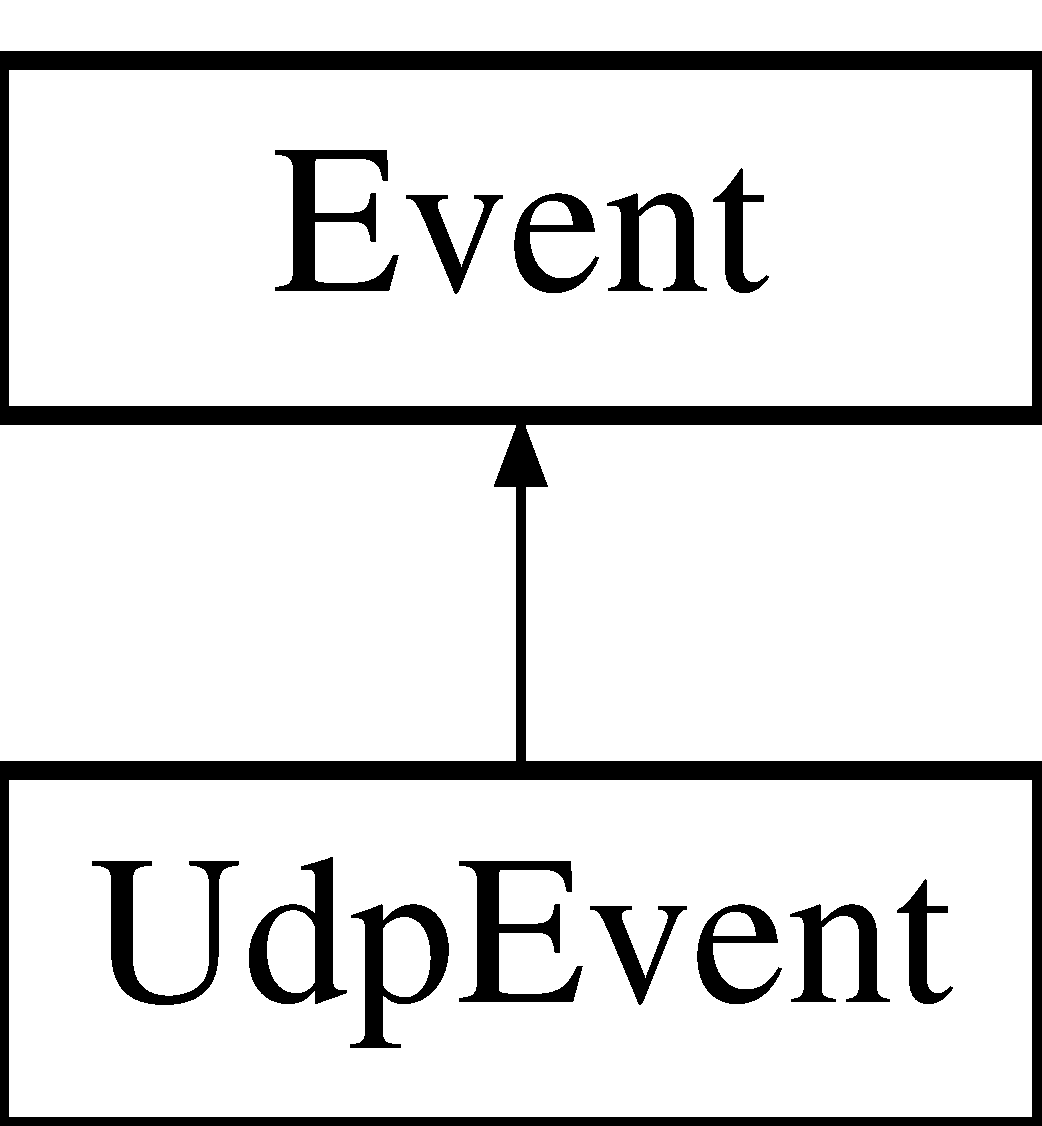
\includegraphics[height=2.000000cm]{classUdpEvent}
\end{center}
\end{figure}
\subsection*{Public Member Functions}
\begin{DoxyCompactItemize}
\item 
\hyperlink{classUdpEvent_aca86b9eaaa735d1a5111045ce8b4d72d}{UdpEvent} (\hyperlink{classUdp}{Udp} $\ast$udp, boost::shared\_\-ptr$<$ udp::socket $>$ \hyperlink{classUdpEvent_ae0cb6d3007132d3a2481d094d009793a}{socket}, boost::shared\_\-ptr$<$ udp::endpoint $>$ \hyperlink{classUdpEvent_a50389e8d457b8f3cc425d78a5d416288}{endpoint}, string \hyperlink{classUdpEvent_a20b7ebd90eb5b21aa7658e3e77ecc96c}{data})
\item 
virtual \hyperlink{classUdpEvent_aa2b3a2c6bfe7b65715e9d202a27b4784}{$\sim$UdpEvent} ()
\item 
virtual void \hyperlink{classUdpEvent_a1f88c17a020ccf73a61a40d18b3728a0}{send} (const string \&\hyperlink{classUdpEvent_a20b7ebd90eb5b21aa7658e3e77ecc96c}{data})
\item 
virtual void \hyperlink{classUdpEvent_ac44fcd996dd22e49d7dd7721198f7550}{send\_\-bytes} (const vector$<$ \hyperlink{Event_8h_ae0aa21f6bcb621fe36c2c962aa0452fe}{byte} $>$ \&bytes)
\item 
virtual string \hyperlink{classUdpEvent_a860ceb7a3a8bb6fcd7cb1342d8b7f5c7}{read} () const 
\item 
virtual FB::VariantList \hyperlink{classUdpEvent_ad315a9d5969bc5d38f3d592119cac9ca}{read\_\-bytes} () const 
\item 
virtual string \hyperlink{classUdpEvent_ae2484477a11197f79d46e4ef4b71b839}{get\_\-host} ()
\item 
virtual unsigned short \hyperlink{classUdpEvent_aaad6ade41ef171993364911ed57a3185}{get\_\-port} ()
\end{DoxyCompactItemize}
\subsection*{Private Attributes}
\begin{DoxyCompactItemize}
\item 
string \hyperlink{classUdpEvent_a20b7ebd90eb5b21aa7658e3e77ecc96c}{data}
\item 
bool \hyperlink{classUdpEvent_a72bdcc219c080212438a4c045928c806}{failed}
\item 
string \hyperlink{classUdpEvent_aaff1c85009ef10ecd363043d7565db8f}{host}
\item 
int \hyperlink{classUdpEvent_a80ca416c15e74042c0e9f440931647d1}{port}
\item 
boost::shared\_\-ptr$<$ udp::socket $>$ \hyperlink{classUdpEvent_ae0cb6d3007132d3a2481d094d009793a}{socket}
\item 
boost::shared\_\-ptr$<$ udp::endpoint $>$ \hyperlink{classUdpEvent_a50389e8d457b8f3cc425d78a5d416288}{endpoint}
\item 
\hyperlink{classUdp}{Udp} $\ast$ \hyperlink{classUdpEvent_a36790f09da79074fc7506dfb3fad7013}{udp\_\-object}
\end{DoxyCompactItemize}


\subsection{Detailed Description}
A UDP implementation of a event to allow javascript to respond to data on a UDP connection.

\begin{DoxySeeAlso}{See also}
\hyperlink{classEvent}{Event} 
\end{DoxySeeAlso}


Definition at line 21 of file UdpEvent.h.



\subsection{Constructor \& Destructor Documentation}
\hypertarget{classUdpEvent_aca86b9eaaa735d1a5111045ce8b4d72d}{
\index{UdpEvent@{UdpEvent}!UdpEvent@{UdpEvent}}
\index{UdpEvent@{UdpEvent}!UdpEvent@{UdpEvent}}
\subsubsection[{UdpEvent}]{\setlength{\rightskip}{0pt plus 5cm}UdpEvent::UdpEvent (
\begin{DoxyParamCaption}
\item[{{\bf Udp} $\ast$}]{udp, }
\item[{boost::shared\_\-ptr$<$ udp::socket $>$}]{socket, }
\item[{boost::shared\_\-ptr$<$ udp::endpoint $>$}]{endpoint, }
\item[{string}]{data}
\end{DoxyParamCaption}
)}}
\label{classUdpEvent_aca86b9eaaa735d1a5111045ce8b4d72d}
Constructs a new {\ttfamily \hyperlink{classUdpEvent}{UdpEvent}} object containing the UDP connection on which to reply.


\begin{DoxyParams}{Parameters}
{\em udp} & The UDP server or client associated with this event \\
\hline
{\em socket} & The UDP connection on which to reply \\
\hline
{\em endpoint} & The remote endpoint for this UDP event, from which we can find information about the remote host \\
\hline
{\em data} & The data this event was fired from \\
\hline
\end{DoxyParams}


Definition at line 10 of file UdpEvent.cpp.



References Logger::error(), failed, host, and port.


\begin{DoxyCode}
                                                                                 
                                               :
    port(-1), socket(socket), endpoint(endpoint), udp_object(udp_object), failed(
      false), data(data)
{
    // Check to see if any the parameters are null, and log and fail if this occu
      rs
    if (endpoint && udp_object)
    {
        // Initialize only if it's safe
        host = boost::lexical_cast<string>(endpoint->address());
        port = endpoint->port();
    }
    else
    {
        // Fail permanently and log it
        failed = true;

        string message("UDP Event was not properly initialized, permanently faile
      d.");
        Logger::error(message, port, host);
        fire_error(message);
    }
}
\end{DoxyCode}
\hypertarget{classUdpEvent_aa2b3a2c6bfe7b65715e9d202a27b4784}{
\index{UdpEvent@{UdpEvent}!$\sim$UdpEvent@{$\sim$UdpEvent}}
\index{$\sim$UdpEvent@{$\sim$UdpEvent}!UdpEvent@{UdpEvent}}
\subsubsection[{$\sim$UdpEvent}]{\setlength{\rightskip}{0pt plus 5cm}UdpEvent::$\sim$UdpEvent (
\begin{DoxyParamCaption}
{}
\end{DoxyParamCaption}
)\hspace{0.3cm}{\ttfamily  \mbox{[}virtual\mbox{]}}}}
\label{classUdpEvent_aa2b3a2c6bfe7b65715e9d202a27b4784}
Deconstructs the UDP event object, after a single reply. 

Definition at line 31 of file UdpEvent.cpp.


\begin{DoxyCode}
{
    // do not free socket, endpoint or udp here
}
\end{DoxyCode}


\subsection{Member Function Documentation}
\hypertarget{classUdpEvent_ae2484477a11197f79d46e4ef4b71b839}{
\index{UdpEvent@{UdpEvent}!get\_\-host@{get\_\-host}}
\index{get\_\-host@{get\_\-host}!UdpEvent@{UdpEvent}}
\subsubsection[{get\_\-host}]{\setlength{\rightskip}{0pt plus 5cm}string UdpEvent::get\_\-host (
\begin{DoxyParamCaption}
\item[{void}]{}
\end{DoxyParamCaption}
)\hspace{0.3cm}{\ttfamily  \mbox{[}virtual\mbox{]}}}}
\label{classUdpEvent_ae2484477a11197f79d46e4ef4b71b839}
Gets the hostname of the remote endpoint of the UDP connection for this {\ttfamily \hyperlink{classUdpEvent}{UdpEvent}}.

\begin{DoxyReturn}{Returns}
The remote hostname of the UDP connection for this {\ttfamily \hyperlink{classUdpEvent}{UdpEvent}} 
\end{DoxyReturn}


Implements \hyperlink{classEvent_ac3fe62061cb4e4552a91be17031fcc2d}{Event}.



Definition at line 93 of file UdpEvent.cpp.



References host.


\begin{DoxyCode}
{
    return host;
}
\end{DoxyCode}
\hypertarget{classUdpEvent_aaad6ade41ef171993364911ed57a3185}{
\index{UdpEvent@{UdpEvent}!get\_\-port@{get\_\-port}}
\index{get\_\-port@{get\_\-port}!UdpEvent@{UdpEvent}}
\subsubsection[{get\_\-port}]{\setlength{\rightskip}{0pt plus 5cm}unsigned short UdpEvent::get\_\-port (
\begin{DoxyParamCaption}
\item[{void}]{}
\end{DoxyParamCaption}
)\hspace{0.3cm}{\ttfamily  \mbox{[}virtual\mbox{]}}}}
\label{classUdpEvent_aaad6ade41ef171993364911ed57a3185}
Gets the port of the remote endpoint of the UDP connection for this {\ttfamily \hyperlink{classUdpEvent}{UdpEvent}}.

\begin{DoxyReturn}{Returns}
The remote port of the UDP connection for this {\ttfamily \hyperlink{classUdpEvent}{UdpEvent}} 
\end{DoxyReturn}


Implements \hyperlink{classEvent_aa23b8454f931fcbe87ed61f1ec70b8e5}{Event}.



Definition at line 98 of file UdpEvent.cpp.



References port.


\begin{DoxyCode}
{
    return port;
}
\end{DoxyCode}
\hypertarget{classUdpEvent_a860ceb7a3a8bb6fcd7cb1342d8b7f5c7}{
\index{UdpEvent@{UdpEvent}!read@{read}}
\index{read@{read}!UdpEvent@{UdpEvent}}
\subsubsection[{read}]{\setlength{\rightskip}{0pt plus 5cm}string UdpEvent::read (
\begin{DoxyParamCaption}
{}
\end{DoxyParamCaption}
) const\hspace{0.3cm}{\ttfamily  \mbox{[}virtual\mbox{]}}}}
\label{classUdpEvent_a860ceb7a3a8bb6fcd7cb1342d8b7f5c7}
Reads the string data that belongs to this event.

\begin{DoxyReturn}{Returns}
The string data received when this event was fired 
\end{DoxyReturn}


Implements \hyperlink{classEvent_a9e334d69556816ca38a8f21845d2a1cb}{Event}.



Definition at line 76 of file UdpEvent.cpp.



References data.


\begin{DoxyCode}
{
    return data;
}
\end{DoxyCode}
\hypertarget{classUdpEvent_ad315a9d5969bc5d38f3d592119cac9ca}{
\index{UdpEvent@{UdpEvent}!read\_\-bytes@{read\_\-bytes}}
\index{read\_\-bytes@{read\_\-bytes}!UdpEvent@{UdpEvent}}
\subsubsection[{read\_\-bytes}]{\setlength{\rightskip}{0pt plus 5cm}FB::VariantList UdpEvent::read\_\-bytes (
\begin{DoxyParamCaption}
{}
\end{DoxyParamCaption}
) const\hspace{0.3cm}{\ttfamily  \mbox{[}virtual\mbox{]}}}}
\label{classUdpEvent_ad315a9d5969bc5d38f3d592119cac9ca}
Reads the byte data that belongs to this event

\begin{DoxyReturn}{Returns}
The byte data received when this event was fired 
\end{DoxyReturn}


Implements \hyperlink{classEvent_a04fa24d70fb7ec47e50e1a71bcedfe75}{Event}.



Definition at line 81 of file UdpEvent.cpp.



References data.


\begin{DoxyCode}
{
    FB::VariantList fb_bytes;

    for (int i = 0; i < data.size(); i++)
    {
        fb_bytes.push_back((unsigned char) (data.data())[i]);
    }

    return fb_bytes;
}
\end{DoxyCode}
\hypertarget{classUdpEvent_a1f88c17a020ccf73a61a40d18b3728a0}{
\index{UdpEvent@{UdpEvent}!send@{send}}
\index{send@{send}!UdpEvent@{UdpEvent}}
\subsubsection[{send}]{\setlength{\rightskip}{0pt plus 5cm}void UdpEvent::send (
\begin{DoxyParamCaption}
\item[{const string \&}]{data}
\end{DoxyParamCaption}
)\hspace{0.3cm}{\ttfamily  \mbox{[}virtual\mbox{]}}}}
\label{classUdpEvent_a1f88c17a020ccf73a61a40d18b3728a0}
Replies on the UDP connection with some data.


\begin{DoxyParams}{Parameters}
{\em data} & The data with which to reply \\
\hline
\end{DoxyParams}


Implements \hyperlink{classEvent_ac4eac8e7d44356632b59381929c8978c}{Event}.



Definition at line 48 of file UdpEvent.cpp.



References endpoint, Logger::error(), Udp::failed, failed, host, Udp::pending\_\-sends, port, Udp::send\_\-handler(), socket, and udp\_\-object.



Referenced by send\_\-bytes().


\begin{DoxyCode}
{
    // Don't send if we've permanently failed
    if (failed)
    {
        string message("UDP event failed to send, Event already failed permanentl
      y");
        Logger::error(message, port, host);
        fire_error(message);
        return;
    }

    if (udp_object && udp_object->failed)
    {
        // Log & fire an error
        string message("UDP event failed trying to reply to a UDP object that has
       permanently failed!");
        Logger::error(message, port, host);
        fire_error(message);
        return;
    }

    if (socket && endpoint)
    {
        udp_object->pending_sends++;
        socket->async_send_to(boost::asio::buffer(data.data(), data.size()), *
      endpoint, 
                boost::bind(&Udp::send_handler, udp_object, _1, _2, data, host, 
      endpoint->port()));
    }
}
\end{DoxyCode}
\hypertarget{classUdpEvent_ac44fcd996dd22e49d7dd7721198f7550}{
\index{UdpEvent@{UdpEvent}!send\_\-bytes@{send\_\-bytes}}
\index{send\_\-bytes@{send\_\-bytes}!UdpEvent@{UdpEvent}}
\subsubsection[{send\_\-bytes}]{\setlength{\rightskip}{0pt plus 5cm}void UdpEvent::send\_\-bytes (
\begin{DoxyParamCaption}
\item[{const vector$<$ {\bf byte} $>$ \&}]{bytes}
\end{DoxyParamCaption}
)\hspace{0.3cm}{\ttfamily  \mbox{[}virtual\mbox{]}}}}
\label{classUdpEvent_ac44fcd996dd22e49d7dd7721198f7550}
Replies on the UDP connection with some data.


\begin{DoxyParams}{Parameters}
{\em bytes} & The bytes of data with which to reply \\
\hline
\end{DoxyParams}


Implements \hyperlink{classEvent_ac2183e14a4f65b18d046a5e082f68e71}{Event}.



Definition at line 36 of file UdpEvent.cpp.



References data, and send().


\begin{DoxyCode}
{
    string data;

    for (int i = 0; i < bytes.size(); i++)
    {
        data.push_back((unsigned char) bytes[i]);
    }

    send(data);
}
\end{DoxyCode}


\subsection{Member Data Documentation}
\hypertarget{classUdpEvent_a20b7ebd90eb5b21aa7658e3e77ecc96c}{
\index{UdpEvent@{UdpEvent}!data@{data}}
\index{data@{data}!UdpEvent@{UdpEvent}}
\subsubsection[{data}]{\setlength{\rightskip}{0pt plus 5cm}string {\bf UdpEvent::data}\hspace{0.3cm}{\ttfamily  \mbox{[}private\mbox{]}}}}
\label{classUdpEvent_a20b7ebd90eb5b21aa7658e3e77ecc96c}
The data received when this event was fired 

Definition at line 88 of file UdpEvent.h.



Referenced by read(), read\_\-bytes(), send\_\-bytes(), and UdpClient::send\_\-bytes().

\hypertarget{classUdpEvent_a50389e8d457b8f3cc425d78a5d416288}{
\index{UdpEvent@{UdpEvent}!endpoint@{endpoint}}
\index{endpoint@{endpoint}!UdpEvent@{UdpEvent}}
\subsubsection[{endpoint}]{\setlength{\rightskip}{0pt plus 5cm}boost::shared\_\-ptr$<$udp::endpoint$>$ {\bf UdpEvent::endpoint}\hspace{0.3cm}{\ttfamily  \mbox{[}private\mbox{]}}}}
\label{classUdpEvent_a50389e8d457b8f3cc425d78a5d416288}
The remote endpoint for this event 

Definition at line 113 of file UdpEvent.h.



Referenced by send().

\hypertarget{classUdpEvent_a72bdcc219c080212438a4c045928c806}{
\index{UdpEvent@{UdpEvent}!failed@{failed}}
\index{failed@{failed}!UdpEvent@{UdpEvent}}
\subsubsection[{failed}]{\setlength{\rightskip}{0pt plus 5cm}bool {\bf UdpEvent::failed}\hspace{0.3cm}{\ttfamily  \mbox{[}private\mbox{]}}}}
\label{classUdpEvent_a72bdcc219c080212438a4c045928c806}
A flag to prevent this event from blowing up if was initialized improperly 

Definition at line 93 of file UdpEvent.h.



Referenced by send(), and UdpEvent().

\hypertarget{classUdpEvent_aaff1c85009ef10ecd363043d7565db8f}{
\index{UdpEvent@{UdpEvent}!host@{host}}
\index{host@{host}!UdpEvent@{UdpEvent}}
\subsubsection[{host}]{\setlength{\rightskip}{0pt plus 5cm}string {\bf UdpEvent::host}\hspace{0.3cm}{\ttfamily  \mbox{[}private\mbox{]}}}}
\label{classUdpEvent_aaff1c85009ef10ecd363043d7565db8f}
The remote hostname of the UDP connection for this {\ttfamily \hyperlink{classUdpEvent}{UdpEvent}} 

Definition at line 98 of file UdpEvent.h.



Referenced by get\_\-host(), send(), and UdpEvent().

\hypertarget{classUdpEvent_a80ca416c15e74042c0e9f440931647d1}{
\index{UdpEvent@{UdpEvent}!port@{port}}
\index{port@{port}!UdpEvent@{UdpEvent}}
\subsubsection[{port}]{\setlength{\rightskip}{0pt plus 5cm}int {\bf UdpEvent::port}\hspace{0.3cm}{\ttfamily  \mbox{[}private\mbox{]}}}}
\label{classUdpEvent_a80ca416c15e74042c0e9f440931647d1}
The remote port of the UDP connection for this {\ttfamily \hyperlink{classUdpEvent}{UdpEvent}} 

Definition at line 103 of file UdpEvent.h.



Referenced by get\_\-port(), send(), and UdpEvent().

\hypertarget{classUdpEvent_ae0cb6d3007132d3a2481d094d009793a}{
\index{UdpEvent@{UdpEvent}!socket@{socket}}
\index{socket@{socket}!UdpEvent@{UdpEvent}}
\subsubsection[{socket}]{\setlength{\rightskip}{0pt plus 5cm}boost::shared\_\-ptr$<$udp::socket$>$ {\bf UdpEvent::socket}\hspace{0.3cm}{\ttfamily  \mbox{[}private\mbox{]}}}}
\label{classUdpEvent_ae0cb6d3007132d3a2481d094d009793a}
The socket corresponding to this UDP 'connection', on which to reply 

Definition at line 108 of file UdpEvent.h.



Referenced by send().

\hypertarget{classUdpEvent_a36790f09da79074fc7506dfb3fad7013}{
\index{UdpEvent@{UdpEvent}!udp\_\-object@{udp\_\-object}}
\index{udp\_\-object@{udp\_\-object}!UdpEvent@{UdpEvent}}
\subsubsection[{udp\_\-object}]{\setlength{\rightskip}{0pt plus 5cm}{\bf Udp}$\ast$ {\bf UdpEvent::udp\_\-object}\hspace{0.3cm}{\ttfamily  \mbox{[}private\mbox{]}}}}
\label{classUdpEvent_a36790f09da79074fc7506dfb3fad7013}
The UDP server or client associated with this event 

Definition at line 118 of file UdpEvent.h.



Referenced by send().



The documentation for this class was generated from the following files:\begin{DoxyCompactItemize}
\item 
/home/jtedesco/dev/sockit/src/udp/\hyperlink{UdpEvent_8h}{UdpEvent.h}\item 
/home/jtedesco/dev/sockit/src/udp/\hyperlink{UdpEvent_8cpp}{UdpEvent.cpp}\end{DoxyCompactItemize}

\hypertarget{classUdpServer}{
\section{UdpServer Class Reference}
\label{classUdpServer}\index{UdpServer@{UdpServer}}
}


{\ttfamily \#include $<$UdpServer.h$>$}

Inheritance diagram for UdpServer:\begin{figure}[H]
\begin{center}
\leavevmode
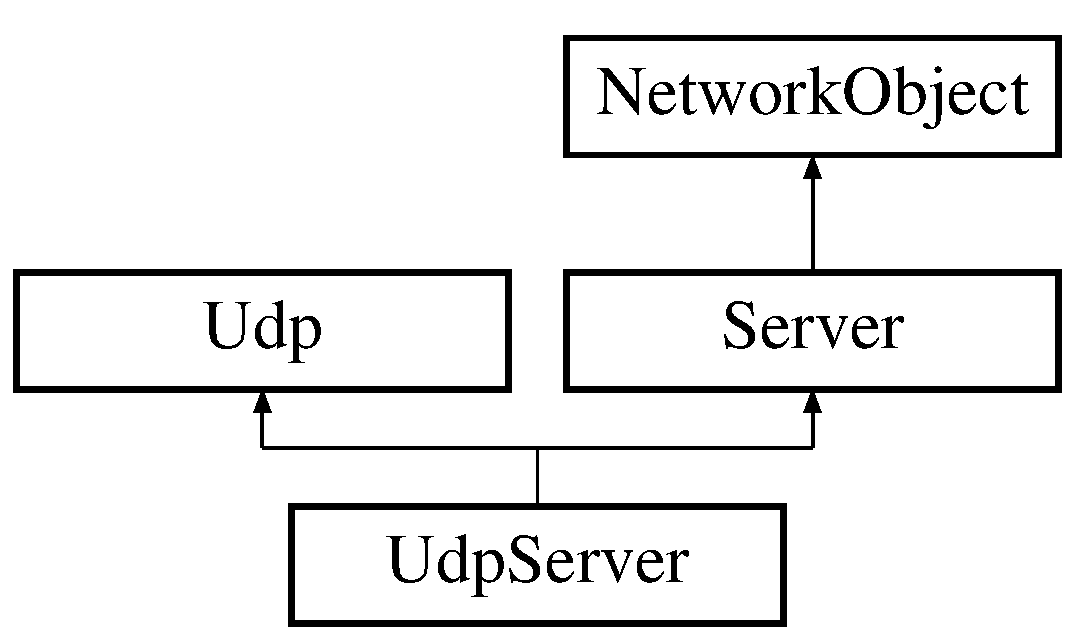
\includegraphics[height=3.000000cm]{classUdpServer}
\end{center}
\end{figure}
\subsection*{Public Member Functions}
\begin{DoxyCompactItemize}
\item 
\hyperlink{classUdpServer_afa92e10874c8a72188a3e1016aad97dc}{UdpServer} (int \hyperlink{classUdp_af69ea781b31a1fa62e5d3012b6288dc8}{port}, boost::asio::io\_\-service \&\hyperlink{classUdp_a7e143116ab3a0f478c8461ca04af782b}{io\_\-service})
\item 
\hyperlink{classUdpServer_ae8a101d8343c9906e42a3fa4bf25e7eb}{UdpServer} (int \hyperlink{classUdp_af69ea781b31a1fa62e5d3012b6288dc8}{port}, boost::asio::io\_\-service \&\hyperlink{classUdp_a7e143116ab3a0f478c8461ca04af782b}{io\_\-service}, map$<$ string, string $>$ options)
\item 
\hyperlink{classUdpServer_aef1871384fbc46ef425242be4474af3a}{$\sim$UdpServer} ()
\item 
virtual void \hyperlink{classUdpServer_a55e557d344720286fdeb430ae3cb3842}{start\_\-listening} ()
\item 
virtual void \hyperlink{classUdpServer_ac5623ca24bc56b21d608426f5bc8ad91}{shutdown} ()
\item 
virtual int \hyperlink{classUdpServer_a276c64a7545b49b298ca3d9ca1a12e9d}{get\_\-port} ()
\end{DoxyCompactItemize}
\subsection*{Protected Member Functions}
\begin{DoxyCompactItemize}
\item 
virtual void \hyperlink{classUdpServer_aa9a023a74c61ba03af476f12958385df}{fire\_\-error\_\-event} (const string \&message)
\item 
virtual void \hyperlink{classUdpServer_ab3bcedec1031181a7dd3affddf3d8447}{fire\_\-data\_\-event} (const string data, boost::shared\_\-ptr$<$ udp::socket $>$ \hyperlink{classUdpServer_a0d49aeb5d5e8291f45487c1d2d082cee}{socket}, boost::shared\_\-ptr$<$ udp::endpoint $>$ endpoint)
\item 
virtual void \hyperlink{classUdpServer_a020144da72e1f29be85ed99225372b21}{close} ()
\end{DoxyCompactItemize}
\subsection*{Private Member Functions}
\begin{DoxyCompactItemize}
\item 
\hyperlink{classUdpServer_a61cfe5dd591450b5486225ab3524bbce}{UdpServer} (const \hyperlink{classUdpServer}{UdpServer} \&other)
\item 
void \hyperlink{classUdpServer_ad5e78e7f2bf29df163003de78fb1c44e}{initialize} (void)
\item 
virtual void \hyperlink{classUdpServer_ad1c4a040a4c510ecd85b9b9c7e61e995}{listen} (void)
\end{DoxyCompactItemize}
\subsection*{Private Attributes}
\begin{DoxyCompactItemize}
\item 
boost::shared\_\-ptr$<$ udp::socket $>$ \hyperlink{classUdpServer_a0d49aeb5d5e8291f45487c1d2d082cee}{socket}
\item 
bool \hyperlink{classUdpServer_a57c16849cfe745828a022aa7346d40d7}{listening}
\end{DoxyCompactItemize}
\subsection*{Friends}
\begin{DoxyCompactItemize}
\item 
class \hyperlink{classUdpServer_aa3db591e179836aff8d4a6d952d43101}{UdpEvent}
\end{DoxyCompactItemize}


\subsection{Detailed Description}
This class represents a UDP server, which inherits basic UDP handling functionality from {\ttfamily \hyperlink{classUdp}{Udp}}, and defines additional functionality to bind to a port and accept incoming connections. 

Definition at line 25 of file UdpServer.h.



\subsection{Constructor \& Destructor Documentation}
\hypertarget{classUdpServer_afa92e10874c8a72188a3e1016aad97dc}{
\index{UdpServer@{UdpServer}!UdpServer@{UdpServer}}
\index{UdpServer@{UdpServer}!UdpServer@{UdpServer}}
\subsubsection[{UdpServer}]{\setlength{\rightskip}{0pt plus 5cm}UdpServer::UdpServer (
\begin{DoxyParamCaption}
\item[{int}]{port, }
\item[{boost::asio::io\_\-service \&}]{io\_\-service}
\end{DoxyParamCaption}
)}}
\label{classUdpServer_afa92e10874c8a72188a3e1016aad97dc}
A constructor that creates a UDP server using IPv4. There are two constructors to satisfy Boost's requirement that sockets are initialized are the initialization list, and to provide the option for using either IPv4 and IPv6. This initializes a UDP server but does not start it listening for incoming connections.


\begin{DoxyParams}{Parameters}
{\em port} & The port on which this UDP server should listen \\
\hline
{\em io\_\-service} & The I/O service to use for asynchronous I/O requests \\
\hline
\end{DoxyParams}


Definition at line 11 of file UdpServer.cpp.



References initialize().


\begin{DoxyCode}
    : Udp("SERVER", port, io_service), socket(new udp::socket(io_service))
{
    initialize();
}
\end{DoxyCode}
\hypertarget{classUdpServer_ae8a101d8343c9906e42a3fa4bf25e7eb}{
\index{UdpServer@{UdpServer}!UdpServer@{UdpServer}}
\index{UdpServer@{UdpServer}!UdpServer@{UdpServer}}
\subsubsection[{UdpServer}]{\setlength{\rightskip}{0pt plus 5cm}UdpServer::UdpServer (
\begin{DoxyParamCaption}
\item[{int}]{port, }
\item[{boost::asio::io\_\-service \&}]{io\_\-service, }
\item[{map$<$ string, string $>$}]{options}
\end{DoxyParamCaption}
)}}
\label{classUdpServer_ae8a101d8343c9906e42a3fa4bf25e7eb}
A constructor that creates a UDP server using IPv6. There are two constructors to satisfy Boost's requirement that sockets are initialized are the initialization list, and to provide the option for using either IPv4 and IPv6. This initializes a UDP server but does not start it listening for incoming connections.


\begin{DoxyParams}{Parameters}
{\em port} & The port on which this UDP server should listen \\
\hline
{\em io\_\-service} & The I/O service to use for asynchronous I/O requests \\
\hline
{\em options} & A map of additional options to configure this UDP server \\
\hline
\end{DoxyParams}


Definition at line 18 of file UdpServer.cpp.



References initialize(), and Udp::parse\_\-args().


\begin{DoxyCode}
    : Udp("SERVER", port, io_service), socket(new udp::socket(io_service))
{
    parse_args(options);

    initialize();
}
\end{DoxyCode}
\hypertarget{classUdpServer_aef1871384fbc46ef425242be4474af3a}{
\index{UdpServer@{UdpServer}!$\sim$UdpServer@{$\sim$UdpServer}}
\index{$\sim$UdpServer@{$\sim$UdpServer}!UdpServer@{UdpServer}}
\subsubsection[{$\sim$UdpServer}]{\setlength{\rightskip}{0pt plus 5cm}UdpServer::$\sim$UdpServer (
\begin{DoxyParamCaption}
{}
\end{DoxyParamCaption}
)}}
\label{classUdpServer_aef1871384fbc46ef425242be4474af3a}
Deconstructs a UDP server, immediately closing the incoming socket and pending operations. 

Definition at line 119 of file UdpServer.cpp.



References close().


\begin{DoxyCode}
{
    close();
}
\end{DoxyCode}
\hypertarget{classUdpServer_a61cfe5dd591450b5486225ab3524bbce}{
\index{UdpServer@{UdpServer}!UdpServer@{UdpServer}}
\index{UdpServer@{UdpServer}!UdpServer@{UdpServer}}
\subsubsection[{UdpServer}]{\setlength{\rightskip}{0pt plus 5cm}UdpServer::UdpServer (
\begin{DoxyParamCaption}
\item[{const {\bf UdpServer} \&}]{other}
\end{DoxyParamCaption}
)\hspace{0.3cm}{\ttfamily  \mbox{[}private\mbox{]}}}}
\label{classUdpServer_a61cfe5dd591450b5486225ab3524bbce}
Disallows copying a UDP server. 

\subsection{Member Function Documentation}
\hypertarget{classUdpServer_a020144da72e1f29be85ed99225372b21}{
\index{UdpServer@{UdpServer}!close@{close}}
\index{close@{close}!UdpServer@{UdpServer}}
\subsubsection[{close}]{\setlength{\rightskip}{0pt plus 5cm}void UdpServer::close (
\begin{DoxyParamCaption}
{}
\end{DoxyParamCaption}
)\hspace{0.3cm}{\ttfamily  \mbox{[}protected, virtual\mbox{]}}}}
\label{classUdpServer_a020144da72e1f29be85ed99225372b21}
Immediately closes the incoming socket \& acceptor, and stops all pending operations. 

Implements \hyperlink{classUdp_a035ec772c3af57eba9d69cf3ba9dcdda}{Udp}.



Definition at line 47 of file UdpServer.cpp.



References socket.



Referenced by shutdown(), and $\sim$UdpServer().


\begin{DoxyCode}
{
    /*
    if (socket->is_open())
    {
        if(multicast && multicast_group)
        {
            socket->set_option(
                    boost::asio::ip::multicast::leave_group(
                        boost::asio::ip::address::from_string(*multicast_group)))
      ;
        }

        socket->close();
    }
    */
    if(socket->is_open())
        socket->close();
}
\end{DoxyCode}
\hypertarget{classUdpServer_ab3bcedec1031181a7dd3affddf3d8447}{
\index{UdpServer@{UdpServer}!fire\_\-data\_\-event@{fire\_\-data\_\-event}}
\index{fire\_\-data\_\-event@{fire\_\-data\_\-event}!UdpServer@{UdpServer}}
\subsubsection[{fire\_\-data\_\-event}]{\setlength{\rightskip}{0pt plus 5cm}void UdpServer::fire\_\-data\_\-event (
\begin{DoxyParamCaption}
\item[{const string}]{data, }
\item[{boost::shared\_\-ptr$<$ udp::socket $>$}]{socket, }
\item[{boost::shared\_\-ptr$<$ udp::endpoint $>$}]{endpoint}
\end{DoxyParamCaption}
)\hspace{0.3cm}{\ttfamily  \mbox{[}protected, virtual\mbox{]}}}}
\label{classUdpServer_ab3bcedec1031181a7dd3affddf3d8447}
Helper to fire data event to javascript.


\begin{DoxyParams}{Parameters}
{\em data} & The data received \\
\hline
{\em socket} & The socket on which to reply to this data \\
\hline
{\em endpoint} & The connected endpoint to the remote host \\
\hline
\end{DoxyParams}


Implements \hyperlink{classUdp_a08e6e588781ce1e7a4d643b97d63dc5c}{Udp}.



Definition at line 213 of file UdpServer.cpp.


\begin{DoxyCode}
{
    fire_data(boost::make_shared<UdpEvent>(this, socket, endpoint, data));
}
\end{DoxyCode}
\hypertarget{classUdpServer_aa9a023a74c61ba03af476f12958385df}{
\index{UdpServer@{UdpServer}!fire\_\-error\_\-event@{fire\_\-error\_\-event}}
\index{fire\_\-error\_\-event@{fire\_\-error\_\-event}!UdpServer@{UdpServer}}
\subsubsection[{fire\_\-error\_\-event}]{\setlength{\rightskip}{0pt plus 5cm}void UdpServer::fire\_\-error\_\-event (
\begin{DoxyParamCaption}
\item[{const string \&}]{message}
\end{DoxyParamCaption}
)\hspace{0.3cm}{\ttfamily  \mbox{[}protected, virtual\mbox{]}}}}
\label{classUdpServer_aa9a023a74c61ba03af476f12958385df}
Helper to fire an error event to javascript.


\begin{DoxyParams}{Parameters}
{\em message} & The error message \\
\hline
\end{DoxyParams}


Implements \hyperlink{classUdp_a9b79c3603ee9196623aa93b505bda1f6}{Udp}.



Definition at line 207 of file UdpServer.cpp.


\begin{DoxyCode}
{
    fire_error(message);
}
\end{DoxyCode}
\hypertarget{classUdpServer_a276c64a7545b49b298ca3d9ca1a12e9d}{
\index{UdpServer@{UdpServer}!get\_\-port@{get\_\-port}}
\index{get\_\-port@{get\_\-port}!UdpServer@{UdpServer}}
\subsubsection[{get\_\-port}]{\setlength{\rightskip}{0pt plus 5cm}int UdpServer::get\_\-port (
\begin{DoxyParamCaption}
\item[{void}]{}
\end{DoxyParamCaption}
)\hspace{0.3cm}{\ttfamily  \mbox{[}virtual\mbox{]}}}}
\label{classUdpServer_a276c64a7545b49b298ca3d9ca1a12e9d}
Returns the port on which this server listens 

Implements \hyperlink{classServer_abd497ca7e7dc29f8ea4c6ce204839a6d}{Server}.



Definition at line 201 of file UdpServer.cpp.



References Udp::port.


\begin{DoxyCode}
{
    return port;
}
\end{DoxyCode}
\hypertarget{classUdpServer_ad5e78e7f2bf29df163003de78fb1c44e}{
\index{UdpServer@{UdpServer}!initialize@{initialize}}
\index{initialize@{initialize}!UdpServer@{UdpServer}}
\subsubsection[{initialize}]{\setlength{\rightskip}{0pt plus 5cm}void UdpServer::initialize (
\begin{DoxyParamCaption}
\item[{void}]{}
\end{DoxyParamCaption}
)\hspace{0.3cm}{\ttfamily  \mbox{[}private\mbox{]}}}}
\label{classUdpServer_ad5e78e7f2bf29df163003de78fb1c44e}
Helper function to initialize this UDP server's object by exposing the {\ttfamily start\_\-listening} method to javascript as 'listen'. 

Definition at line 67 of file UdpServer.cpp.



References Udp::BUFFER\_\-SIZE, Udp::do\_\-not\_\-route, Logger::error(), Udp::host, listening, Udp::log\_\-options(), Udp::multicast, Udp::multicast\_\-ttl, Udp::port, Udp::reuse\_\-address, socket, start\_\-listening(), and Udp::using\_\-ipv6.



Referenced by UdpServer().


\begin{DoxyCode}
{
    log_options();

    listening = false;

    if(using_ipv6 && *using_ipv6)
        socket->open(udp::v6());
    else
        socket->open(udp::v4());

    if(!socket->is_open())
    {
        string message("UDP server failed to initialize, could not open socket");
      
        Logger::error(message, port, host);
        fire_error(message);
    }

    // synchronize the buffer size of the socket with this class's buffer size
    boost::asio::socket_base::receive_buffer_size buf_size_option(BUFFER_SIZE);
    socket->set_option(buf_size_option);

    if(do_not_route)
    {
        boost::asio::socket_base::do_not_route option(*do_not_route);
        socket->set_option(option);
    }

    if(reuse_address)
    {
        boost::asio::socket_base::reuse_address option(*reuse_address);
        socket->set_option(option);
    }

    if(multicast)
    {
        /* force this to be set */
        boost::asio::socket_base::reuse_address option(true);
        socket->set_option(option);
    }

    if(multicast_ttl)
    {
        boost::asio::ip::multicast::hops option(*multicast_ttl);
        socket->set_option(option);
    }

    // register these methods so they can be invoked from the Javascript
    registerMethod("listen", make_method(this, &UdpServer::start_listening));
}
\end{DoxyCode}
\hypertarget{classUdpServer_ad1c4a040a4c510ecd85b9b9c7e61e995}{
\index{UdpServer@{UdpServer}!listen@{listen}}
\index{listen@{listen}!UdpServer@{UdpServer}}
\subsubsection[{listen}]{\setlength{\rightskip}{0pt plus 5cm}void UdpServer::listen (
\begin{DoxyParamCaption}
\item[{void}]{}
\end{DoxyParamCaption}
)\hspace{0.3cm}{\ttfamily  \mbox{[}private, virtual\mbox{]}}}}
\label{classUdpServer_ad1c4a040a4c510ecd85b9b9c7e61e995}
Helper function to listen for new data from incoming connections. 

Implements \hyperlink{classUdp_a645a7a67007362e349cacc78f9870954}{Udp}.



Definition at line 190 of file UdpServer.cpp.



References Udp::host, Logger::info(), Udp::port, Udp::receive\_\-buffer, Udp::receive\_\-handler(), Udp::remote\_\-endpoint, socket, and Logger::warn().



Referenced by start\_\-listening().


\begin{DoxyCode}
{
    Logger::info("udpserver: starting to listen", port, host);

    if(remote_endpoint && remote_endpoint.get())
        socket->async_receive_from(boost::asio::buffer(receive_buffer), *
      remote_endpoint,
                boost::bind(&UdpServer::receive_handler, this, _1, _2, socket, 
      remote_endpoint, host, port));
    else
        Logger::warn("remote endpoint is null", port, host);
}
\end{DoxyCode}
\hypertarget{classUdpServer_ac5623ca24bc56b21d608426f5bc8ad91}{
\index{UdpServer@{UdpServer}!shutdown@{shutdown}}
\index{shutdown@{shutdown}!UdpServer@{UdpServer}}
\subsubsection[{shutdown}]{\setlength{\rightskip}{0pt plus 5cm}void UdpServer::shutdown (
\begin{DoxyParamCaption}
{}
\end{DoxyParamCaption}
)\hspace{0.3cm}{\ttfamily  \mbox{[}virtual\mbox{]}}}}
\label{classUdpServer_ac5623ca24bc56b21d608426f5bc8ad91}
Gracefully shutdown this UDP server, waiting until all sends have completed before freeing all resources for this UDP server and shutting down any open connections. This function is exposed the javascript API. 

Implements \hyperlink{classNetworkObject_a2f519457fd87c8a92cf265a2b2883e96}{NetworkObject}.



Definition at line 27 of file UdpServer.cpp.



References close(), Logger::error(), Udp::failed, Udp::host, Udp::pending\_\-sends, Udp::port, and Udp::should\_\-close.


\begin{DoxyCode}
{
    if(!failed)
    {
        should_close = true;

        if (pending_sends == 0) {
            fire_close();
            close();
        }
    }
    else
    {
        // Log & fire an error
        string message("Trying to shutdown a permanently failed UDP server!");
        Logger::error(message, port, host);
    }

}
\end{DoxyCode}
\hypertarget{classUdpServer_a55e557d344720286fdeb430ae3cb3842}{
\index{UdpServer@{UdpServer}!start\_\-listening@{start\_\-listening}}
\index{start\_\-listening@{start\_\-listening}!UdpServer@{UdpServer}}
\subsubsection[{start\_\-listening}]{\setlength{\rightskip}{0pt plus 5cm}void UdpServer::start\_\-listening (
\begin{DoxyParamCaption}
{}
\end{DoxyParamCaption}
)\hspace{0.3cm}{\ttfamily  \mbox{[}virtual\mbox{]}}}}
\label{classUdpServer_a55e557d344720286fdeb430ae3cb3842}
Called to start the the server listening for the first time, fires the 'open' event, and is exposed to the javascript. This should only be called once, and starts the server listening for incoming connections. 

Implements \hyperlink{classServer_ab60269481230955b94dc6405162794b0}{Server}.



Definition at line 125 of file UdpServer.cpp.



References Logger::error(), Udp::failed, Udp::host, Logger::info(), listen(), listening, Udp::multicast, Udp::multicast\_\-group, Udp::port, socket, and Udp::using\_\-ipv6.



Referenced by initialize().


\begin{DoxyCode}
{
    if(failed)
    {
        // Log & fire an error
        string message("Trying to start a UDP server that has permanently failed!
      ");
        Logger::error(message, port, host);
        return;
    }

    if(listening) return;

    try
    {
        if(using_ipv6 && *using_ipv6)
            socket->bind(udp::endpoint(udp::v6(), port));
        else
            socket->bind(udp::endpoint(udp::v4(), port));
    }
    catch (boost::system::system_error &e)
    {
        // Catch this error, and fail gracefully
        string message(string("Caught error initializing UDP server: '") + e.what
      () + "'");
        Logger::error(message, port, host);

        // Stop this server from ever doing anything again
        failed = true;
        return;
    }

    Logger::info("bind!", port, host);

    if(multicast)
    {
        if(!multicast_group)
        {
            Logger::error("UdpServer: Multicast set, but no multicast group given
      ", port, host);
        }
        else
        {
            // Try to join the multicast group, and fail gracefully if we can't j
      oin it
            try
            {
                socket->set_option(boost::asio::ip::multicast::join_group(
                            boost::asio::ip::address::from_string(*
      multicast_group)));
            }
            catch(boost::system::system_error & error)
            {
                // Catch this error, and fail gracefully
                string message(string("Caught error initializing UDP joinging mul
      ticast group: '") + error.what() + "'");
                Logger::error(message, port, host);

                failed = true;
                return;
            }
        }
    }

    listen();
    fire_open();

    listening = true;
}
\end{DoxyCode}


\subsection{Friends And Related Function Documentation}
\hypertarget{classUdpServer_aa3db591e179836aff8d4a6d952d43101}{
\index{UdpServer@{UdpServer}!UdpEvent@{UdpEvent}}
\index{UdpEvent@{UdpEvent}!UdpServer@{UdpServer}}
\subsubsection[{UdpEvent}]{\setlength{\rightskip}{0pt plus 5cm}friend class {\bf UdpEvent}\hspace{0.3cm}{\ttfamily  \mbox{[}friend\mbox{]}}}}
\label{classUdpServer_aa3db591e179836aff8d4a6d952d43101}


Reimplemented from \hyperlink{classUdp_aa3db591e179836aff8d4a6d952d43101}{Udp}.



Definition at line 73 of file UdpServer.h.



\subsection{Member Data Documentation}
\hypertarget{classUdpServer_a57c16849cfe745828a022aa7346d40d7}{
\index{UdpServer@{UdpServer}!listening@{listening}}
\index{listening@{listening}!UdpServer@{UdpServer}}
\subsubsection[{listening}]{\setlength{\rightskip}{0pt plus 5cm}bool {\bf UdpServer::listening}\hspace{0.3cm}{\ttfamily  \mbox{[}private\mbox{]}}}}
\label{classUdpServer_a57c16849cfe745828a022aa7346d40d7}
A flag to indicate this object is already listening 

Definition at line 122 of file UdpServer.h.



Referenced by initialize(), and start\_\-listening().

\hypertarget{classUdpServer_a0d49aeb5d5e8291f45487c1d2d082cee}{
\index{UdpServer@{UdpServer}!socket@{socket}}
\index{socket@{socket}!UdpServer@{UdpServer}}
\subsubsection[{socket}]{\setlength{\rightskip}{0pt plus 5cm}boost::shared\_\-ptr$<$udp::socket$>$ {\bf UdpServer::socket}\hspace{0.3cm}{\ttfamily  \mbox{[}private\mbox{]}}}}
\label{classUdpServer_a0d49aeb5d5e8291f45487c1d2d082cee}
The socket for incoming communications to this server. 

Definition at line 119 of file UdpServer.h.



Referenced by close(), initialize(), listen(), and start\_\-listening().



The documentation for this class was generated from the following files:\begin{DoxyCompactItemize}
\item 
/home/jtedesco/dev/sockit/src/udp/\hyperlink{UdpServer_8h}{UdpServer.h}\item 
/home/jtedesco/dev/sockit/src/udp/\hyperlink{UdpServer_8cpp}{UdpServer.cpp}\end{DoxyCompactItemize}

\chapter{File Documentation}
\hypertarget{Client_8cpp}{
\section{/home/jtedesco/dev/sockit/src/common/Client.cpp File Reference}
\label{Client_8cpp}\index{/home/jtedesco/dev/sockit/src/common/Client.cpp@{/home/jtedesco/dev/sockit/src/common/Client.cpp}}
}
{\ttfamily \#include \char`\"{}Client.h\char`\"{}}\par

\hypertarget{Client_8h}{
\section{/home/jtedesco/dev/sockit/src/common/Client.h File Reference}
\label{Client_8h}\index{/home/jtedesco/dev/sockit/src/common/Client.h@{/home/jtedesco/dev/sockit/src/common/Client.h}}
}
{\ttfamily \#include \char`\"{}NetworkObject.h\char`\"{}}\par
\subsection*{Classes}
\begin{DoxyCompactItemize}
\item 
class \hyperlink{classClient}{Client}
\end{DoxyCompactItemize}

\hypertarget{Event_8cpp}{
\section{/home/jtedesco/dev/sockit/src/common/Event.cpp File Reference}
\label{Event_8cpp}\index{/home/jtedesco/dev/sockit/src/common/Event.cpp@{/home/jtedesco/dev/sockit/src/common/Event.cpp}}
}
{\ttfamily \#include \char`\"{}Event.h\char`\"{}}\par

\hypertarget{Event_8h}{
\section{/home/jtedesco/dev/sockit/src/common/Event.h File Reference}
\label{Event_8h}\index{/home/jtedesco/dev/sockit/src/common/Event.h@{/home/jtedesco/dev/sockit/src/common/Event.h}}
}
{\ttfamily \#include $<$string$>$}\par
{\ttfamily \#include $<$vector$>$}\par
{\ttfamily \#include $<$boost/asio.hpp$>$}\par
{\ttfamily \#include \char`\"{}JSAPIAuto.h\char`\"{}}\par
\subsection*{Classes}
\begin{DoxyCompactItemize}
\item 
class \hyperlink{classEvent}{Event}
\end{DoxyCompactItemize}
\subsection*{Typedefs}
\begin{DoxyCompactItemize}
\item 
typedef uint16\_\-t \hyperlink{Event_8h_ae0aa21f6bcb621fe36c2c962aa0452fe}{byte}
\item 
typedef wstring \hyperlink{Event_8h_a42e68af8ed186972f3b40e079e28dfb1}{binary}
\end{DoxyCompactItemize}


\subsection{Typedef Documentation}
\hypertarget{Event_8h_a42e68af8ed186972f3b40e079e28dfb1}{
\index{Event.h@{Event.h}!binary@{binary}}
\index{binary@{binary}!Event.h@{Event.h}}
\subsubsection[{binary}]{\setlength{\rightskip}{0pt plus 5cm}typedef wstring {\bf binary}}}
\label{Event_8h_a42e68af8ed186972f3b40e079e28dfb1}


Definition at line 24 of file Event.h.

\hypertarget{Event_8h_ae0aa21f6bcb621fe36c2c962aa0452fe}{
\index{Event.h@{Event.h}!byte@{byte}}
\index{byte@{byte}!Event.h@{Event.h}}
\subsubsection[{byte}]{\setlength{\rightskip}{0pt plus 5cm}typedef uint16\_\-t {\bf byte}}}
\label{Event_8h_ae0aa21f6bcb621fe36c2c962aa0452fe}


Definition at line 23 of file Event.h.


\hypertarget{NetworkObject_8cpp}{
\section{/home/jtedesco/dev/sockit/src/common/NetworkObject.cpp File Reference}
\label{NetworkObject_8cpp}\index{/home/jtedesco/dev/sockit/src/common/NetworkObject.cpp@{/home/jtedesco/dev/sockit/src/common/NetworkObject.cpp}}
}
{\ttfamily \#include \char`\"{}NetworkObject.h\char`\"{}}\par

\hypertarget{NetworkObject_8h}{
\section{/home/jtedesco/dev/sockit/src/common/NetworkObject.h File Reference}
\label{NetworkObject_8h}\index{/home/jtedesco/dev/sockit/src/common/NetworkObject.h@{/home/jtedesco/dev/sockit/src/common/NetworkObject.h}}
}
{\ttfamily \#include $<$string$>$}\par
{\ttfamily \#include $<$map$>$}\par
{\ttfamily \#include $<$vector$>$}\par
{\ttfamily \#include $<$queue$>$}\par
{\ttfamily \#include \char`\"{}JSAPIAuto.h\char`\"{}}\par
\subsection*{Classes}
\begin{DoxyCompactItemize}
\item 
class \hyperlink{classNetworkObject}{NetworkObject}
\end{DoxyCompactItemize}
\subsection*{Typedefs}
\begin{DoxyCompactItemize}
\item 
typedef uint16\_\-t \hyperlink{NetworkObject_8h_ae0aa21f6bcb621fe36c2c962aa0452fe}{byte}
\item 
typedef wstring \hyperlink{NetworkObject_8h_a42e68af8ed186972f3b40e079e28dfb1}{binary}
\end{DoxyCompactItemize}


\subsection{Typedef Documentation}
\hypertarget{NetworkObject_8h_a42e68af8ed186972f3b40e079e28dfb1}{
\index{NetworkObject.h@{NetworkObject.h}!binary@{binary}}
\index{binary@{binary}!NetworkObject.h@{NetworkObject.h}}
\subsubsection[{binary}]{\setlength{\rightskip}{0pt plus 5cm}typedef wstring {\bf binary}}}
\label{NetworkObject_8h_a42e68af8ed186972f3b40e079e28dfb1}


Definition at line 51 of file NetworkObject.h.

\hypertarget{NetworkObject_8h_ae0aa21f6bcb621fe36c2c962aa0452fe}{
\index{NetworkObject.h@{NetworkObject.h}!byte@{byte}}
\index{byte@{byte}!NetworkObject.h@{NetworkObject.h}}
\subsubsection[{byte}]{\setlength{\rightskip}{0pt plus 5cm}typedef uint16\_\-t {\bf byte}}}
\label{NetworkObject_8h_ae0aa21f6bcb621fe36c2c962aa0452fe}


Definition at line 50 of file NetworkObject.h.


\hypertarget{NetworkThread_8cpp}{
\section{/home/jtedesco/dev/sockit/src/common/NetworkThread.cpp File Reference}
\label{NetworkThread_8cpp}\index{/home/jtedesco/dev/sockit/src/common/NetworkThread.cpp@{/home/jtedesco/dev/sockit/src/common/NetworkThread.cpp}}
}
{\ttfamily \#include \char`\"{}NetworkThread.h\char`\"{}}\par

\hypertarget{NetworkThread_8h}{
\section{/home/jtedesco/dev/sockit/src/common/NetworkThread.h File Reference}
\label{NetworkThread_8h}\index{/home/jtedesco/dev/sockit/src/common/NetworkThread.h@{/home/jtedesco/dev/sockit/src/common/NetworkThread.h}}
}
{\ttfamily \#include $<$boost/weak\_\-ptr.hpp$>$}\par
{\ttfamily \#include $<$boost/lexical\_\-cast.hpp$>$}\par
{\ttfamily \#include $<$map$>$}\par
{\ttfamily \#include $<$set$>$}\par
{\ttfamily \#include $<$string$>$}\par
{\ttfamily \#include \char`\"{}JSAPIAuto.h\char`\"{}}\par
{\ttfamily \#include \char`\"{}TcpClient.h\char`\"{}}\par
{\ttfamily \#include \char`\"{}TcpEvent.h\char`\"{}}\par
{\ttfamily \#include \char`\"{}TcpServer.h\char`\"{}}\par
{\ttfamily \#include \char`\"{}UdpClient.h\char`\"{}}\par
{\ttfamily \#include \char`\"{}UdpEvent.h\char`\"{}}\par
{\ttfamily \#include \char`\"{}UdpServer.h\char`\"{}}\par
\subsection*{Classes}
\begin{DoxyCompactItemize}
\item 
class \hyperlink{classNetworkThread}{NetworkThread}
\end{DoxyCompactItemize}

\hypertarget{Server_8cpp}{
\section{/home/jtedesco/dev/sockit/src/common/Server.cpp File Reference}
\label{Server_8cpp}\index{/home/jtedesco/dev/sockit/src/common/Server.cpp@{/home/jtedesco/dev/sockit/src/common/Server.cpp}}
}
{\ttfamily \#include \char`\"{}Server.h\char`\"{}}\par

\hypertarget{Server_8h}{
\section{/home/jtedesco/dev/sockit/src/common/Server.h File Reference}
\label{Server_8h}\index{/home/jtedesco/dev/sockit/src/common/Server.h@{/home/jtedesco/dev/sockit/src/common/Server.h}}
}
{\ttfamily \#include \char`\"{}NetworkObject.h\char`\"{}}\par
\subsection*{Classes}
\begin{DoxyCompactItemize}
\item 
class \hyperlink{classServer}{Server}
\end{DoxyCompactItemize}

\hypertarget{Logger_8cpp}{
\section{/home/jtedesco/dev/sockit/src/logger/Logger.cpp File Reference}
\label{Logger_8cpp}\index{/home/jtedesco/dev/sockit/src/logger/Logger.cpp@{/home/jtedesco/dev/sockit/src/logger/Logger.cpp}}
}
{\ttfamily \#include \char`\"{}Logger.h\char`\"{}}\par
\subsection*{Defines}
\begin{DoxyCompactItemize}
\item 
\#define \hyperlink{Logger_8cpp_afa36afb199484fd6c9b906c8ccca9ed9}{PROFILE\_\-BUF\_\-LEN}~250
\end{DoxyCompactItemize}


\subsection{Define Documentation}
\hypertarget{Logger_8cpp_afa36afb199484fd6c9b906c8ccca9ed9}{
\index{Logger.cpp@{Logger.cpp}!PROFILE\_\-BUF\_\-LEN@{PROFILE\_\-BUF\_\-LEN}}
\index{PROFILE\_\-BUF\_\-LEN@{PROFILE\_\-BUF\_\-LEN}!Logger.cpp@{Logger.cpp}}
\subsubsection[{PROFILE\_\-BUF\_\-LEN}]{\setlength{\rightskip}{0pt plus 5cm}\#define PROFILE\_\-BUF\_\-LEN~250}}
\label{Logger_8cpp_afa36afb199484fd6c9b906c8ccca9ed9}


Referenced by Logger::get\_\-log\_\-base\_\-path().


\hypertarget{Logger_8h}{
\section{/home/jtedesco/dev/sockit/src/logger/Logger.h File Reference}
\label{Logger_8h}\index{/home/jtedesco/dev/sockit/src/logger/Logger.h@{/home/jtedesco/dev/sockit/src/logger/Logger.h}}
}
{\ttfamily \#include \char`\"{}process.h\char`\"{}}\par
{\ttfamily \#include $<$winsock2.h$>$}\par
{\ttfamily \#include $<$windows.h$>$}\par
{\ttfamily \#include $<$conio.h$>$}\par
{\ttfamily \#include $<$stdio.h$>$}\par
{\ttfamily \#include $<$queue$>$}\par
{\ttfamily \#include $<$string$>$}\par
{\ttfamily \#include $<$boost/date\_\-time/local\_\-time/local\_\-time.hpp$>$}\par
{\ttfamily \#include $<$boost/date\_\-time/posix\_\-time/posix\_\-time.hpp$>$}\par
{\ttfamily \#include $<$boost/filesystem.hpp$>$}\par
{\ttfamily \#include $<$boost/lexical\_\-cast.hpp$>$}\par
{\ttfamily \#include $<$boost/thread.hpp$>$}\par
\subsection*{Classes}
\begin{DoxyCompactItemize}
\item 
class \hyperlink{classLogger}{Logger}
\end{DoxyCompactItemize}
\subsection*{Defines}
\begin{DoxyCompactItemize}
\item 
\#define \hyperlink{Logger_8h_ac7bef5d85e3dcd73eef56ad39ffc84a9}{WIN32\_\-LEAN\_\-AND\_\-MEAN}
\item 
\#define \hyperlink{Logger_8h_a1230649f2e178a83485c5b5465ff8260}{PID}~\_\-getpid()
\end{DoxyCompactItemize}


\subsection{Define Documentation}
\hypertarget{Logger_8h_a1230649f2e178a83485c5b5465ff8260}{
\index{Logger.h@{Logger.h}!PID@{PID}}
\index{PID@{PID}!Logger.h@{Logger.h}}
\subsubsection[{PID}]{\setlength{\rightskip}{0pt plus 5cm}\#define PID~\_\-getpid()}}
\label{Logger_8h_a1230649f2e178a83485c5b5465ff8260}


Definition at line 16 of file Logger.h.

\hypertarget{Logger_8h_ac7bef5d85e3dcd73eef56ad39ffc84a9}{
\index{Logger.h@{Logger.h}!WIN32\_\-LEAN\_\-AND\_\-MEAN@{WIN32\_\-LEAN\_\-AND\_\-MEAN}}
\index{WIN32\_\-LEAN\_\-AND\_\-MEAN@{WIN32\_\-LEAN\_\-AND\_\-MEAN}!Logger.h@{Logger.h}}
\subsubsection[{WIN32\_\-LEAN\_\-AND\_\-MEAN}]{\setlength{\rightskip}{0pt plus 5cm}\#define WIN32\_\-LEAN\_\-AND\_\-MEAN}}
\label{Logger_8h_ac7bef5d85e3dcd73eef56ad39ffc84a9}


Definition at line 11 of file Logger.h.


\hypertarget{Factory_8cpp}{
\section{/home/jtedesco/dev/sockit/src/plugin/Factory.cpp File Reference}
\label{Factory_8cpp}\index{/home/jtedesco/dev/sockit/src/plugin/Factory.cpp@{/home/jtedesco/dev/sockit/src/plugin/Factory.cpp}}
}
{\ttfamily \#include \char`\"{}FactoryBase.h\char`\"{}}\par
{\ttfamily \#include \char`\"{}SockIt.h\char`\"{}}\par
{\ttfamily \#include $<$boost/make\_\-shared.hpp$>$}\par
\subsection*{Classes}
\begin{DoxyCompactItemize}
\item 
class \hyperlink{classPluginFactory}{PluginFactory}
\end{DoxyCompactItemize}
\subsection*{Functions}
\begin{DoxyCompactItemize}
\item 
FB::FactoryBasePtr \hyperlink{Factory_8cpp_a0c0e10db1382088eb360b06c1c839c69}{getFactoryInstance} ()
\begin{DoxyCompactList}\small\item\em Returns the factory instance for this plugin module. \item\end{DoxyCompactList}\end{DoxyCompactItemize}


\subsection{Function Documentation}
\hypertarget{Factory_8cpp_a0c0e10db1382088eb360b06c1c839c69}{
\index{Factory.cpp@{Factory.cpp}!getFactoryInstance@{getFactoryInstance}}
\index{getFactoryInstance@{getFactoryInstance}!Factory.cpp@{Factory.cpp}}
\subsubsection[{getFactoryInstance}]{\setlength{\rightskip}{0pt plus 5cm}getFactoryInstance (
\begin{DoxyParamCaption}
{}
\end{DoxyParamCaption}
)}}
\label{Factory_8cpp_a0c0e10db1382088eb360b06c1c839c69}


Returns the factory instance for this plugin module. 



Definition at line 54 of file Factory.cpp.


\begin{DoxyCode}
{
    static boost::shared_ptr<PluginFactory> factory = boost::make_shared<PluginFa
      ctory>();
    return factory;
}
\end{DoxyCode}

\hypertarget{SockIt_8cpp}{
\section{/home/jtedesco/dev/sockit/src/plugin/SockIt.cpp File Reference}
\label{SockIt_8cpp}\index{/home/jtedesco/dev/sockit/src/plugin/SockIt.cpp@{/home/jtedesco/dev/sockit/src/plugin/SockIt.cpp}}
}
{\ttfamily \#include \char`\"{}SockItAPI.h\char`\"{}}\par
{\ttfamily \#include \char`\"{}SockIt.h\char`\"{}}\par

\hypertarget{SockIt_8h}{
\section{/home/jtedesco/dev/sockit/src/plugin/SockIt.h File Reference}
\label{SockIt_8h}\index{/home/jtedesco/dev/sockit/src/plugin/SockIt.h@{/home/jtedesco/dev/sockit/src/plugin/SockIt.h}}
}
{\ttfamily \#include \char`\"{}PluginWindow.h\char`\"{}}\par
{\ttfamily \#include \char`\"{}PluginEvents/MouseEvents.h\char`\"{}}\par
{\ttfamily \#include \char`\"{}PluginEvents/AttachedEvent.h\char`\"{}}\par
{\ttfamily \#include \char`\"{}PluginCore.h\char`\"{}}\par
{\ttfamily \#include \char`\"{}Logger.h\char`\"{}}\par
\subsection*{Classes}
\begin{DoxyCompactItemize}
\item 
class \hyperlink{classSockIt}{SockIt}
\end{DoxyCompactItemize}

\hypertarget{SockItAPI_8cpp}{
\section{/home/jtedesco/dev/sockit/src/plugin/SockItAPI.cpp File Reference}
\label{SockItAPI_8cpp}\index{/home/jtedesco/dev/sockit/src/plugin/SockItAPI.cpp@{/home/jtedesco/dev/sockit/src/plugin/SockItAPI.cpp}}
}
{\ttfamily \#include \char`\"{}JSObject.h\char`\"{}}\par
{\ttfamily \#include \char`\"{}variant\_\-list.h\char`\"{}}\par
{\ttfamily \#include \char`\"{}DOM/Document.h\char`\"{}}\par
{\ttfamily \#include \char`\"{}SockItAPI.h\char`\"{}}\par

\hypertarget{SockItAPI_8h}{
\section{/home/jtedesco/dev/sockit/src/plugin/SockItAPI.h File Reference}
\label{SockItAPI_8h}\index{/home/jtedesco/dev/sockit/src/plugin/SockItAPI.h@{/home/jtedesco/dev/sockit/src/plugin/SockItAPI.h}}
}
{\ttfamily \#include $<$map$>$}\par
{\ttfamily \#include $<$string$>$}\par
{\ttfamily \#include $<$sstream$>$}\par
{\ttfamily \#include $<$vector$>$}\par
{\ttfamily \#include $<$boost/optional.hpp$>$}\par
{\ttfamily \#include $<$boost/weak\_\-ptr.hpp$>$}\par
{\ttfamily \#include $<$stdint.h$>$}\par
{\ttfamily \#include \char`\"{}BrowserHost.h\char`\"{}}\par
{\ttfamily \#include \char`\"{}JSAPIAuto.h\char`\"{}}\par
{\ttfamily \#include \char`\"{}SockIt.h\char`\"{}}\par
{\ttfamily \#include \char`\"{}NetworkThread.h\char`\"{}}\par
\subsection*{Classes}
\begin{DoxyCompactItemize}
\item 
class \hyperlink{classSockItAPI}{SockItAPI}
\end{DoxyCompactItemize}

\hypertarget{Tcp_8cpp}{
\section{/home/jtedesco/dev/sockit/src/tcp/Tcp.cpp File Reference}
\label{Tcp_8cpp}\index{/home/jtedesco/dev/sockit/src/tcp/Tcp.cpp@{/home/jtedesco/dev/sockit/src/tcp/Tcp.cpp}}
}
{\ttfamily \#include \char`\"{}Tcp.h\char`\"{}}\par

\hypertarget{Tcp_8h}{
\section{/home/jtedesco/dev/sockit/src/tcp/Tcp.h File Reference}
\label{Tcp_8h}\index{/home/jtedesco/dev/sockit/src/tcp/Tcp.h@{/home/jtedesco/dev/sockit/src/tcp/Tcp.h}}
}
{\ttfamily \#include $<$boost/asio.hpp$>$}\par
{\ttfamily \#include $<$boost/thread.hpp$>$}\par
{\ttfamily \#include $<$boost/make\_\-shared.hpp$>$}\par
{\ttfamily \#include $<$boost/lexical\_\-cast.hpp$>$}\par
{\ttfamily \#include $<$boost/optional.hpp$>$}\par
{\ttfamily \#include $<$iostream$>$}\par
{\ttfamily \#include $<$set$>$}\par
{\ttfamily \#include $<$map$>$}\par
{\ttfamily \#include $<$winsock2.h$>$}\par
{\ttfamily \#include $<$Windows.h$>$}\par
{\ttfamily \#include $<$MSTcpIP.h$>$}\par
{\ttfamily \#include \char`\"{}TcpEvent.h\char`\"{}}\par
{\ttfamily \#include \char`\"{}Logger.h\char`\"{}}\par
\subsection*{Classes}
\begin{DoxyCompactItemize}
\item 
class \hyperlink{classTcp}{Tcp}
\end{DoxyCompactItemize}
\subsection*{Defines}
\begin{DoxyCompactItemize}
\item 
\#define \hyperlink{Tcp_8h_ac7bef5d85e3dcd73eef56ad39ffc84a9}{WIN32\_\-LEAN\_\-AND\_\-MEAN}
\end{DoxyCompactItemize}


\subsection{Define Documentation}
\hypertarget{Tcp_8h_ac7bef5d85e3dcd73eef56ad39ffc84a9}{
\index{Tcp.h@{Tcp.h}!WIN32\_\-LEAN\_\-AND\_\-MEAN@{WIN32\_\-LEAN\_\-AND\_\-MEAN}}
\index{WIN32\_\-LEAN\_\-AND\_\-MEAN@{WIN32\_\-LEAN\_\-AND\_\-MEAN}!Tcp.h@{Tcp.h}}
\subsubsection[{WIN32\_\-LEAN\_\-AND\_\-MEAN}]{\setlength{\rightskip}{0pt plus 5cm}\#define WIN32\_\-LEAN\_\-AND\_\-MEAN}}
\label{Tcp_8h_ac7bef5d85e3dcd73eef56ad39ffc84a9}


Definition at line 36 of file Tcp.h.


\hypertarget{TcpClient_8cpp}{
\section{/home/jtedesco/dev/sockit/src/tcp/TcpClient.cpp File Reference}
\label{TcpClient_8cpp}\index{/home/jtedesco/dev/sockit/src/tcp/TcpClient.cpp@{/home/jtedesco/dev/sockit/src/tcp/TcpClient.cpp}}
}
{\ttfamily \#include \char`\"{}TcpClient.h\char`\"{}}\par

\hypertarget{TcpClient_8h}{
\section{/home/jtedesco/dev/sockit/src/tcp/TcpClient.h File Reference}
\label{TcpClient_8h}\index{/home/jtedesco/dev/sockit/src/tcp/TcpClient.h@{/home/jtedesco/dev/sockit/src/tcp/TcpClient.h}}
}
{\ttfamily \#include $<$boost/lexical\_\-cast.hpp$>$}\par
{\ttfamily \#include $<$boost/thread.hpp$>$}\par
{\ttfamily \#include $<$string.h$>$}\par
{\ttfamily \#include \char`\"{}Client.h\char`\"{}}\par
{\ttfamily \#include \char`\"{}Logger.h\char`\"{}}\par
{\ttfamily \#include \char`\"{}Tcp.h\char`\"{}}\par
\subsection*{Classes}
\begin{DoxyCompactItemize}
\item 
class \hyperlink{classTcpClient}{TcpClient}
\end{DoxyCompactItemize}

\hypertarget{TcpEvent_8cpp}{
\section{/home/jtedesco/dev/sockit/src/tcp/TcpEvent.cpp File Reference}
\label{TcpEvent_8cpp}\index{/home/jtedesco/dev/sockit/src/tcp/TcpEvent.cpp@{/home/jtedesco/dev/sockit/src/tcp/TcpEvent.cpp}}
}
{\ttfamily \#include \char`\"{}TcpEvent.h\char`\"{}}\par
{\ttfamily \#include $<$stdio.h$>$}\par

\hypertarget{TcpEvent_8h}{
\section{/home/jtedesco/dev/sockit/src/tcp/TcpEvent.h File Reference}
\label{TcpEvent_8h}\index{/home/jtedesco/dev/sockit/src/tcp/TcpEvent.h@{/home/jtedesco/dev/sockit/src/tcp/TcpEvent.h}}
}
{\ttfamily \#include $<$boost/asio.hpp$>$}\par
{\ttfamily \#include \char`\"{}JSAPIAuto.h\char`\"{}}\par
{\ttfamily \#include \char`\"{}Event.h\char`\"{}}\par
{\ttfamily \#include \char`\"{}Tcp.h\char`\"{}}\par
\subsection*{Classes}
\begin{DoxyCompactItemize}
\item 
class \hyperlink{classTcpEvent}{TcpEvent}
\end{DoxyCompactItemize}

\hypertarget{TcpServer_8cpp}{
\section{/home/jtedesco/dev/sockit/src/tcp/TcpServer.cpp File Reference}
\label{TcpServer_8cpp}\index{/home/jtedesco/dev/sockit/src/tcp/TcpServer.cpp@{/home/jtedesco/dev/sockit/src/tcp/TcpServer.cpp}}
}
{\ttfamily \#include \char`\"{}TcpServer.h\char`\"{}}\par
\subsection*{Functions}
\begin{DoxyCompactItemize}
\item 
void \hyperlink{TcpServer_8cpp_ac9dd6924c09e22e8976648dfb53b9d77}{socket\_\-deallocate} (tcp::socket $\ast$socket)
\end{DoxyCompactItemize}


\subsection{Function Documentation}
\hypertarget{TcpServer_8cpp_ac9dd6924c09e22e8976648dfb53b9d77}{
\index{TcpServer.cpp@{TcpServer.cpp}!socket\_\-deallocate@{socket\_\-deallocate}}
\index{socket\_\-deallocate@{socket\_\-deallocate}!TcpServer.cpp@{TcpServer.cpp}}
\subsubsection[{socket\_\-deallocate}]{\setlength{\rightskip}{0pt plus 5cm}void socket\_\-deallocate (
\begin{DoxyParamCaption}
\item[{tcp::socket $\ast$}]{socket}
\end{DoxyParamCaption}
)}}
\label{TcpServer_8cpp_ac9dd6924c09e22e8976648dfb53b9d77}
Helper function to shutdown and deallocate the memory for a socket.


\begin{DoxyParams}{Parameters}
{\em socket} & The socket to deallocate. \\
\hline
\end{DoxyParams}


Definition at line 138 of file TcpServer.cpp.



References Logger::error().



Referenced by TcpServer::start\_\-listening().


\begin{DoxyCode}
{
    // may already have been deallocated
    if(!socket) return;

    try
    {
        if(socket && socket->is_open())
        {
            //s->shutdown(s->shutdown_both);
            socket->close();
        }
    }
    catch(boost::system::error_code &e)
    {
        Logger::error("socket deallocate: " + e.message());
    }
    catch(std::exception &er)
    {
        Logger::error("socket deallocate: " + std::string(er.what()));
    }

    delete socket;
    socket = 0;
}
\end{DoxyCode}

\hypertarget{TcpServer_8h}{
\section{/home/jtedesco/dev/sockit/src/tcp/TcpServer.h File Reference}
\label{TcpServer_8h}\index{/home/jtedesco/dev/sockit/src/tcp/TcpServer.h@{/home/jtedesco/dev/sockit/src/tcp/TcpServer.h}}
}
{\ttfamily \#include $<$set$>$}\par
{\ttfamily \#include \char`\"{}Tcp.h\char`\"{}}\par
{\ttfamily \#include \char`\"{}Server.h\char`\"{}}\par
{\ttfamily \#include \char`\"{}Logger.h\char`\"{}}\par
\subsection*{Classes}
\begin{DoxyCompactItemize}
\item 
class \hyperlink{classTcpServer}{TcpServer}
\end{DoxyCompactItemize}

\hypertarget{Udp_8cpp}{
\section{/home/jtedesco/dev/sockit/src/udp/Udp.cpp File Reference}
\label{Udp_8cpp}\index{/home/jtedesco/dev/sockit/src/udp/Udp.cpp@{/home/jtedesco/dev/sockit/src/udp/Udp.cpp}}
}
{\ttfamily \#include \char`\"{}Udp.h\char`\"{}}\par

\hypertarget{Udp_8h}{
\section{/home/jtedesco/dev/sockit/src/udp/Udp.h File Reference}
\label{Udp_8h}\index{/home/jtedesco/dev/sockit/src/udp/Udp.h@{/home/jtedesco/dev/sockit/src/udp/Udp.h}}
}
{\ttfamily \#include $<$boost/asio.hpp$>$}\par
{\ttfamily \#include $<$boost/asio/buffer.hpp$>$}\par
{\ttfamily \#include $<$boost/lexical\_\-cast.hpp$>$}\par
{\ttfamily \#include $<$boost/make\_\-shared.hpp$>$}\par
{\ttfamily \#include $<$boost/optional.hpp$>$}\par
{\ttfamily \#include $<$boost/thread.hpp$>$}\par
{\ttfamily \#include $<$map$>$}\par
{\ttfamily \#include \char`\"{}UdpEvent.h\char`\"{}}\par
{\ttfamily \#include \char`\"{}Logger.h\char`\"{}}\par
\subsection*{Classes}
\begin{DoxyCompactItemize}
\item 
class \hyperlink{classUdp}{Udp}
\end{DoxyCompactItemize}
\subsection*{Typedefs}
\begin{DoxyCompactItemize}
\item 
typedef boost::asio::const\_\-buffers\_\-1 \hyperlink{Udp_8h_aa0155849c020a1db7cc2ce5d741eb44a}{boost\_\-buffer}
\end{DoxyCompactItemize}


\subsection{Typedef Documentation}
\hypertarget{Udp_8h_aa0155849c020a1db7cc2ce5d741eb44a}{
\index{Udp.h@{Udp.h}!boost\_\-buffer@{boost\_\-buffer}}
\index{boost\_\-buffer@{boost\_\-buffer}!Udp.h@{Udp.h}}
\subsubsection[{boost\_\-buffer}]{\setlength{\rightskip}{0pt plus 5cm}typedef boost::asio::const\_\-buffers\_\-1 {\bf boost\_\-buffer}}}
\label{Udp_8h_aa0155849c020a1db7cc2ce5d741eb44a}


Definition at line 31 of file Udp.h.


\hypertarget{UdpClient_8cpp}{
\section{/home/jtedesco/dev/sockit/src/udp/UdpClient.cpp File Reference}
\label{UdpClient_8cpp}\index{/home/jtedesco/dev/sockit/src/udp/UdpClient.cpp@{/home/jtedesco/dev/sockit/src/udp/UdpClient.cpp}}
}
{\ttfamily \#include \char`\"{}UdpClient.h\char`\"{}}\par

\hypertarget{UdpClient_8h}{
\section{/home/jtedesco/dev/sockit/src/udp/UdpClient.h File Reference}
\label{UdpClient_8h}\index{/home/jtedesco/dev/sockit/src/udp/UdpClient.h@{/home/jtedesco/dev/sockit/src/udp/UdpClient.h}}
}
{\ttfamily \#include $<$algorithm$>$}\par
{\ttfamily \#include $<$map$>$}\par
{\ttfamily \#include $<$string$>$}\par
{\ttfamily \#include $<$queue$>$}\par
{\ttfamily \#include $<$boost/asio.hpp$>$}\par
{\ttfamily \#include $<$boost/bind.hpp$>$}\par
{\ttfamily \#include $<$boost/thread.hpp$>$}\par
{\ttfamily \#include \char`\"{}Client.h\char`\"{}}\par
{\ttfamily \#include \char`\"{}Logger.h\char`\"{}}\par
{\ttfamily \#include \char`\"{}Event.h\char`\"{}}\par
{\ttfamily \#include \char`\"{}Udp.h\char`\"{}}\par
\subsection*{Classes}
\begin{DoxyCompactItemize}
\item 
class \hyperlink{classUdpClient}{UdpClient}
\end{DoxyCompactItemize}

\hypertarget{UdpEvent_8cpp}{
\section{/home/jtedesco/dev/sockit/src/udp/UdpEvent.cpp File Reference}
\label{UdpEvent_8cpp}\index{/home/jtedesco/dev/sockit/src/udp/UdpEvent.cpp@{/home/jtedesco/dev/sockit/src/udp/UdpEvent.cpp}}
}
{\ttfamily \#include \char`\"{}UdpEvent.h\char`\"{}}\par

\hypertarget{UdpEvent_8h}{
\section{/home/jtedesco/dev/sockit/src/udp/UdpEvent.h File Reference}
\label{UdpEvent_8h}\index{/home/jtedesco/dev/sockit/src/udp/UdpEvent.h@{/home/jtedesco/dev/sockit/src/udp/UdpEvent.h}}
}
{\ttfamily \#include \char`\"{}Event.h\char`\"{}}\par
{\ttfamily \#include \char`\"{}Udp.h\char`\"{}}\par
\subsection*{Classes}
\begin{DoxyCompactItemize}
\item 
class \hyperlink{classUdpEvent}{UdpEvent}
\end{DoxyCompactItemize}

\hypertarget{UdpServer_8cpp}{
\section{/home/jtedesco/dev/sockit/src/udp/UdpServer.cpp File Reference}
\label{UdpServer_8cpp}\index{/home/jtedesco/dev/sockit/src/udp/UdpServer.cpp@{/home/jtedesco/dev/sockit/src/udp/UdpServer.cpp}}
}
{\ttfamily \#include \char`\"{}UdpServer.h\char`\"{}}\par

\hypertarget{UdpServer_8h}{
\section{/home/jtedesco/dev/sockit/src/udp/UdpServer.h File Reference}
\label{UdpServer_8h}\index{/home/jtedesco/dev/sockit/src/udp/UdpServer.h@{/home/jtedesco/dev/sockit/src/udp/UdpServer.h}}
}
{\ttfamily \#include $<$string$>$}\par
{\ttfamily \#include $<$boost/asio.hpp$>$}\par
{\ttfamily \#include $<$boost/bind.hpp$>$}\par
{\ttfamily \#include $<$boost/thread.hpp$>$}\par
{\ttfamily \#include \char`\"{}Udp.h\char`\"{}}\par
{\ttfamily \#include \char`\"{}Server.h\char`\"{}}\par
{\ttfamily \#include \char`\"{}Logger.h\char`\"{}}\par
{\ttfamily \#include \char`\"{}Event.h\char`\"{}}\par
{\ttfamily \#include \char`\"{}UdpEvent.h\char`\"{}}\par
\subsection*{Classes}
\begin{DoxyCompactItemize}
\item 
class \hyperlink{classUdpServer}{UdpServer}
\end{DoxyCompactItemize}

\printindex
\end{document}
